\documentclass[twoside]{book}

% Packages required by doxygen
\usepackage{fixltx2e}
\usepackage{calc}
\usepackage{doxygen}
\usepackage[export]{adjustbox} % also loads graphicx
\usepackage{graphicx}
\usepackage[utf8]{inputenc}
\usepackage{makeidx}
\usepackage{multicol}
\usepackage{multirow}
\PassOptionsToPackage{warn}{textcomp}
\usepackage{textcomp}
\usepackage[nointegrals]{wasysym}
\usepackage[table]{xcolor}

% Font selection
\usepackage[T1]{fontenc}
\usepackage[scaled=.90]{helvet}
\usepackage{courier}
\usepackage{amssymb}
\usepackage{sectsty}
\renewcommand{\familydefault}{\sfdefault}
\allsectionsfont{%
  \fontseries{bc}\selectfont%
  \color{darkgray}%
}
\renewcommand{\DoxyLabelFont}{%
  \fontseries{bc}\selectfont%
  \color{darkgray}%
}
\newcommand{\+}{\discretionary{\mbox{\scriptsize$\hookleftarrow$}}{}{}}

% Page & text layout
\usepackage{geometry}
\geometry{%
  a4paper,%
  top=2.5cm,%
  bottom=2.5cm,%
  left=2.5cm,%
  right=2.5cm%
}
\tolerance=750
\hfuzz=15pt
\hbadness=750
\setlength{\emergencystretch}{15pt}
\setlength{\parindent}{0cm}
\setlength{\parskip}{3ex plus 2ex minus 2ex}
\makeatletter
\renewcommand{\paragraph}{%
  \@startsection{paragraph}{4}{0ex}{-1.0ex}{1.0ex}{%
    \normalfont\normalsize\bfseries\SS@parafont%
  }%
}
\renewcommand{\subparagraph}{%
  \@startsection{subparagraph}{5}{0ex}{-1.0ex}{1.0ex}{%
    \normalfont\normalsize\bfseries\SS@subparafont%
  }%
}
\makeatother

% Headers & footers
\usepackage{fancyhdr}
\pagestyle{fancyplain}
\fancyhead[LE]{\fancyplain{}{\bfseries\thepage}}
\fancyhead[CE]{\fancyplain{}{}}
\fancyhead[RE]{\fancyplain{}{\bfseries\leftmark}}
\fancyhead[LO]{\fancyplain{}{\bfseries\rightmark}}
\fancyhead[CO]{\fancyplain{}{}}
\fancyhead[RO]{\fancyplain{}{\bfseries\thepage}}
\fancyfoot[LE]{\fancyplain{}{}}
\fancyfoot[CE]{\fancyplain{}{}}
\fancyfoot[RE]{\fancyplain{}{\bfseries\scriptsize Generated by Doxygen }}
\fancyfoot[LO]{\fancyplain{}{\bfseries\scriptsize Generated by Doxygen }}
\fancyfoot[CO]{\fancyplain{}{}}
\fancyfoot[RO]{\fancyplain{}{}}
\renewcommand{\footrulewidth}{0.4pt}
\renewcommand{\chaptermark}[1]{%
  \markboth{#1}{}%
}
\renewcommand{\sectionmark}[1]{%
  \markright{\thesection\ #1}%
}

% Indices & bibliography
\usepackage{natbib}
\usepackage[titles]{tocloft}
\setcounter{tocdepth}{3}
\setcounter{secnumdepth}{5}
\makeindex

% Hyperlinks (required, but should be loaded last)
\usepackage{ifpdf}
\ifpdf
  \usepackage[pdftex,pagebackref=true]{hyperref}
\else
  \usepackage[ps2pdf,pagebackref=true]{hyperref}
\fi
\hypersetup{%
  colorlinks=true,%
  linkcolor=blue,%
  citecolor=blue,%
  unicode%
}

% Custom commands
\newcommand{\clearemptydoublepage}{%
  \newpage{\pagestyle{empty}\cleardoublepage}%
}

\usepackage{caption}
\captionsetup{labelsep=space,justification=centering,font={bf},singlelinecheck=off,skip=4pt,position=top}

%===== C O N T E N T S =====

\begin{document}

% Titlepage & ToC
\hypersetup{pageanchor=false,
             bookmarksnumbered=true,
             pdfencoding=unicode
            }
\pagenumbering{alph}
\begin{titlepage}
\vspace*{7cm}
\begin{center}%
{\Large llk\+\_\+tb \\[1ex]\large 0.\+01 }\\
\vspace*{1cm}
{\large Generated by Doxygen 1.8.13}\\
\end{center}
\end{titlepage}
\clearemptydoublepage
\pagenumbering{roman}
\tableofcontents
\clearemptydoublepage
\pagenumbering{arabic}
\hypersetup{pageanchor=true}

%--- Begin generated contents ---
\chapter{Namespace Index}
\section{Namespace List}
Here is a list of all namespaces with brief descriptions\+:\begin{DoxyCompactList}
\item\contentsline{section}{\hyperlink{namespacellk}{llk} }{\pageref{namespacellk}}{}
\item\contentsline{section}{\hyperlink{namespacellk_1_1assemble__kernels}{llk\+::assemble\+\_\+kernels} \\*Assemble\+\_\+kernels meant to assemble and build kernel memories }{\pageref{namespacellk_1_1assemble__kernels}}{}
\item\contentsline{section}{\hyperlink{namespacellk_1_1tensor__ops}{llk\+::tensor\+\_\+ops} }{\pageref{namespacellk_1_1tensor__ops}}{}
\item\contentsline{section}{\hyperlink{namespacellk_1_1tensor__ops_1_1tile__ops}{llk\+::tensor\+\_\+ops\+::tile\+\_\+ops} }{\pageref{namespacellk_1_1tensor__ops_1_1tile__ops}}{}
\item\contentsline{section}{\hyperlink{namespacellk_1_1test__lib}{llk\+::test\+\_\+lib} \\*Test\+\_\+lib is the exposed library functions to interface and interact with tests }{\pageref{namespacellk_1_1test__lib}}{}
\item\contentsline{section}{\hyperlink{namespacestd}{std} }{\pageref{namespacestd}}{}
\item\contentsline{section}{\hyperlink{namespacetests}{tests} }{\pageref{namespacetests}}{}
\item\contentsline{section}{\hyperlink{namespacetests_1_1test__config__api}{tests\+::test\+\_\+config\+\_\+api} }{\pageref{namespacetests_1_1test__config__api}}{}
\end{DoxyCompactList}

\chapter{Class Index}
\section{Class List}
Here are the classes, structs, unions and interfaces with brief descriptions\+:\begin{DoxyCompactList}
\item\contentsline{section}{\hyperlink{structllk_1_1BufferMemory}{llk\+::\+Buffer\+Memory} }{\pageref{structllk_1_1BufferMemory}}{}
\item\contentsline{section}{\hyperlink{structllk_1_1CoreDescriptor}{llk\+::\+Core\+Descriptor} \\*Soc\+Node\+Descriptor contains information regarding the Node/\+Core }{\pageref{structllk_1_1CoreDescriptor}}{}
\item\contentsline{section}{\hyperlink{classllk_1_1Device}{llk\+::\+Device} \\*\hyperlink{classllk_1_1Device}{Device} A\+PI in a wrapper class }{\pageref{classllk_1_1Device}}{}
\item\contentsline{section}{\hyperlink{classllk_1_1discontiguous__hex__file__writer}{llk\+::discontiguous\+\_\+hex\+\_\+file\+\_\+writer} }{\pageref{classllk_1_1discontiguous__hex__file__writer}}{}
\item\contentsline{section}{\hyperlink{structstd_1_1hash_3_01llk_1_1xy__pair_01_4}{std\+::hash$<$ llk\+::xy\+\_\+pair $>$} }{\pageref{structstd_1_1hash_3_01llk_1_1xy__pair_01_4}}{}
\item\contentsline{section}{\hyperlink{structtests_1_1KernelParams}{tests\+::\+Kernel\+Params} }{\pageref{structtests_1_1KernelParams}}{}
\item\contentsline{section}{\hyperlink{classllk_1_1memory}{llk\+::memory} }{\pageref{classllk_1_1memory}}{}
\item\contentsline{section}{\hyperlink{structtests_1_1OverlayConfig}{tests\+::\+Overlay\+Config} }{\pageref{structtests_1_1OverlayConfig}}{}
\item\contentsline{section}{\hyperlink{structtests_1_1SingleCoreTestConfig}{tests\+::\+Single\+Core\+Test\+Config} \\*\hyperlink{structtests_1_1TestConfig}{Test\+Config} specification for a specific core }{\pageref{structtests_1_1SingleCoreTestConfig}}{}
\item\contentsline{section}{\hyperlink{structllk_1_1SocDescriptor}{llk\+::\+Soc\+Descriptor} \\*\hyperlink{structllk_1_1SocDescriptor}{Soc\+Descriptor} contains information regarding the S\+OC configuration targetted }{\pageref{structllk_1_1SocDescriptor}}{}
\item\contentsline{section}{\hyperlink{classllk_1_1Tensor}{llk\+::\+Tensor} }{\pageref{classllk_1_1Tensor}}{}
\item\contentsline{section}{\hyperlink{structtests_1_1TensorConfig}{tests\+::\+Tensor\+Config} }{\pageref{structtests_1_1TensorConfig}}{}
\item\contentsline{section}{\hyperlink{structllk_1_1TensorDims}{llk\+::\+Tensor\+Dims} }{\pageref{structllk_1_1TensorDims}}{}
\item\contentsline{section}{\hyperlink{structllk_1_1test__address__map}{llk\+::test\+\_\+address\+\_\+map} }{\pageref{structllk_1_1test__address__map}}{}
\item\contentsline{section}{\hyperlink{structtests_1_1TestArgs}{tests\+::\+Test\+Args} }{\pageref{structtests_1_1TestArgs}}{}
\item\contentsline{section}{\hyperlink{structtests_1_1TestConfig}{tests\+::\+Test\+Config} \\*\hyperlink{structtests_1_1TestConfig}{Test\+Config} -\/ Config Structure }{\pageref{structtests_1_1TestConfig}}{}
\item\contentsline{section}{\hyperlink{structllk_1_1xy__pair}{llk\+::xy\+\_\+pair} }{\pageref{structllk_1_1xy__pair}}{}
\end{DoxyCompactList}

\chapter{File Index}
\section{File List}
Here is a list of all files with brief descriptions\+:\begin{DoxyCompactList}
\item\contentsline{section}{inc/\hyperlink{llk__addresses_8h}{llk\+\_\+addresses.\+h} }{\pageref{llk__addresses_8h}}{}
\item\contentsline{section}{inc/\hyperlink{llk__assemble__kernels_8h}{llk\+\_\+assemble\+\_\+kernels.\+h} }{\pageref{llk__assemble__kernels_8h}}{}
\item\contentsline{section}{inc/\hyperlink{llk__device_8h}{llk\+\_\+device.\+h} }{\pageref{llk__device_8h}}{}
\item\contentsline{section}{inc/\hyperlink{llk__hexfile_8h}{llk\+\_\+hexfile.\+h} }{\pageref{llk__hexfile_8h}}{}
\item\contentsline{section}{inc/\hyperlink{llk__memory_8h}{llk\+\_\+memory.\+h} }{\pageref{llk__memory_8h}}{}
\item\contentsline{section}{inc/\hyperlink{llk__rounding_8h}{llk\+\_\+rounding.\+h} }{\pageref{llk__rounding_8h}}{}
\item\contentsline{section}{inc/\hyperlink{llk__soc__descriptor_8h}{llk\+\_\+soc\+\_\+descriptor.\+h} }{\pageref{llk__soc__descriptor_8h}}{}
\item\contentsline{section}{inc/\hyperlink{llk__tensor_8h}{llk\+\_\+tensor.\+h} }{\pageref{llk__tensor_8h}}{}
\item\contentsline{section}{inc/\hyperlink{llk__tensor__data__format_8h}{llk\+\_\+tensor\+\_\+data\+\_\+format.\+h} }{\pageref{llk__tensor__data__format_8h}}{}
\item\contentsline{section}{inc/\hyperlink{llk__tensor__dims_8h}{llk\+\_\+tensor\+\_\+dims.\+h} }{\pageref{llk__tensor__dims_8h}}{}
\item\contentsline{section}{inc/\hyperlink{llk__tensor__ops_8h}{llk\+\_\+tensor\+\_\+ops.\+h} }{\pageref{llk__tensor__ops_8h}}{}
\item\contentsline{section}{inc/\hyperlink{llk__tensor__tile__layout_8h}{llk\+\_\+tensor\+\_\+tile\+\_\+layout.\+h} }{\pageref{llk__tensor__tile__layout_8h}}{}
\item\contentsline{section}{inc/\hyperlink{llk__types_8h}{llk\+\_\+types.\+h} }{\pageref{llk__types_8h}}{}
\item\contentsline{section}{inc/\hyperlink{llk__verify_8h}{llk\+\_\+verify.\+h} }{\pageref{llk__verify_8h}}{}
\item\contentsline{section}{inc/\hyperlink{llk__xy__pair_8h}{llk\+\_\+xy\+\_\+pair.\+h} }{\pageref{llk__xy__pair_8h}}{}
\item\contentsline{section}{src/\hyperlink{llk__assemble__kernels_8cpp}{llk\+\_\+assemble\+\_\+kernels.\+cpp} }{\pageref{llk__assemble__kernels_8cpp}}{}
\item\contentsline{section}{src/\hyperlink{llk__device_8cpp}{llk\+\_\+device.\+cpp} }{\pageref{llk__device_8cpp}}{}
\item\contentsline{section}{src/\hyperlink{llk__hexfile_8cpp}{llk\+\_\+hexfile.\+cpp} }{\pageref{llk__hexfile_8cpp}}{}
\item\contentsline{section}{src/\hyperlink{llk__memory_8cpp}{llk\+\_\+memory.\+cpp} }{\pageref{llk__memory_8cpp}}{}
\item\contentsline{section}{src/\hyperlink{llk__soc__descriptor_8cpp}{llk\+\_\+soc\+\_\+descriptor.\+cpp} }{\pageref{llk__soc__descriptor_8cpp}}{}
\item\contentsline{section}{src/\hyperlink{llk__tensor_8cpp}{llk\+\_\+tensor.\+cpp} }{\pageref{llk__tensor_8cpp}}{}
\item\contentsline{section}{src/\hyperlink{llk__tensor__data__format_8cpp}{llk\+\_\+tensor\+\_\+data\+\_\+format.\+cpp} }{\pageref{llk__tensor__data__format_8cpp}}{}
\item\contentsline{section}{src/\hyperlink{llk__tensor__ops_8cpp}{llk\+\_\+tensor\+\_\+ops.\+cpp} }{\pageref{llk__tensor__ops_8cpp}}{}
\item\contentsline{section}{src/\hyperlink{llk__verify_8cpp}{llk\+\_\+verify.\+cpp} }{\pageref{llk__verify_8cpp}}{}
\item\contentsline{section}{src/\hyperlink{llk__xy__pair_8cpp}{llk\+\_\+xy\+\_\+pair.\+cpp} }{\pageref{llk__xy__pair_8cpp}}{}
\item\contentsline{section}{tests/\hyperlink{test__args_8h}{test\+\_\+args.\+h} }{\pageref{test__args_8h}}{}
\item\contentsline{section}{tests/\hyperlink{test__config_8cpp}{test\+\_\+config.\+cpp} }{\pageref{test__config_8cpp}}{}
\item\contentsline{section}{tests/\hyperlink{test__config_8h}{test\+\_\+config.\+h} }{\pageref{test__config_8h}}{}
\item\contentsline{section}{tests/\hyperlink{test__kernel__params_8cpp}{test\+\_\+kernel\+\_\+params.\+cpp} }{\pageref{test__kernel__params_8cpp}}{}
\item\contentsline{section}{tests/\hyperlink{test__kernel__params_8h}{test\+\_\+kernel\+\_\+params.\+h} }{\pageref{test__kernel__params_8h}}{}
\item\contentsline{section}{tests/\hyperlink{test__list_8h}{test\+\_\+list.\+h} }{\pageref{test__list_8h}}{}
\item\contentsline{section}{tests/\hyperlink{test__overlay__config_8cpp}{test\+\_\+overlay\+\_\+config.\+cpp} }{\pageref{test__overlay__config_8cpp}}{}
\item\contentsline{section}{tests/\hyperlink{test__overlay__config_8h}{test\+\_\+overlay\+\_\+config.\+h} }{\pageref{test__overlay__config_8h}}{}
\item\contentsline{section}{tests/\hyperlink{test__tensor__config_8cpp}{test\+\_\+tensor\+\_\+config.\+cpp} }{\pageref{test__tensor__config_8cpp}}{}
\item\contentsline{section}{tests/\hyperlink{test__tensor__config_8h}{test\+\_\+tensor\+\_\+config.\+h} }{\pageref{test__tensor__config_8h}}{}
\item\contentsline{section}{tests/\hyperlink{tests_8h}{tests.\+h} }{\pageref{tests_8h}}{}
\item\contentsline{section}{tests/\hyperlink{tests__lib_8cpp}{tests\+\_\+lib.\+cpp} }{\pageref{tests__lib_8cpp}}{}
\item\contentsline{section}{tests/\hyperlink{tests__lib_8h}{tests\+\_\+lib.\+h} }{\pageref{tests__lib_8h}}{}
\end{DoxyCompactList}

\chapter{Namespace Documentation}
\hypertarget{namespacellk}{}\section{llk Namespace Reference}
\label{namespacellk}\index{llk@{llk}}
\subsection*{Namespaces}
\begin{DoxyCompactItemize}
\item 
 \hyperlink{namespacellk_1_1assemble__kernels}{assemble\+\_\+kernels}
\begin{DoxyCompactList}\small\item\em \hyperlink{namespacellk_1_1assemble__kernels}{assemble\+\_\+kernels} meant to assemble and build kernel memories \end{DoxyCompactList}\item 
 \hyperlink{namespacellk_1_1tensor__ops}{tensor\+\_\+ops}
\item 
 \hyperlink{namespacellk_1_1test__lib}{test\+\_\+lib}
\begin{DoxyCompactList}\small\item\em \hyperlink{namespacellk_1_1test__lib}{test\+\_\+lib} is the exposed library functions to interface and interact with tests \end{DoxyCompactList}\end{DoxyCompactItemize}
\subsection*{Classes}
\begin{DoxyCompactItemize}
\item 
struct \hyperlink{structllk_1_1BufferMemory}{Buffer\+Memory}
\item 
struct \hyperlink{structllk_1_1CoreDescriptor}{Core\+Descriptor}
\begin{DoxyCompactList}\small\item\em Soc\+Node\+Descriptor contains information regarding the Node/\+Core. \end{DoxyCompactList}\item 
class \hyperlink{classllk_1_1Device}{Device}
\begin{DoxyCompactList}\small\item\em \hyperlink{classllk_1_1Device}{Device} A\+PI in a wrapper class. \end{DoxyCompactList}\item 
class \hyperlink{classllk_1_1discontiguous__hex__file__writer}{discontiguous\+\_\+hex\+\_\+file\+\_\+writer}
\item 
class \hyperlink{classllk_1_1memory}{memory}
\item 
struct \hyperlink{structllk_1_1SocDescriptor}{Soc\+Descriptor}
\begin{DoxyCompactList}\small\item\em \hyperlink{structllk_1_1SocDescriptor}{Soc\+Descriptor} contains information regarding the S\+OC configuration targetted. \end{DoxyCompactList}\item 
class \hyperlink{classllk_1_1Tensor}{Tensor}
\item 
struct \hyperlink{structllk_1_1TensorDims}{Tensor\+Dims}
\item 
struct \hyperlink{structllk_1_1test__address__map}{test\+\_\+address\+\_\+map}
\item 
struct \hyperlink{structllk_1_1xy__pair}{xy\+\_\+pair}
\end{DoxyCompactItemize}
\subsection*{Enumerations}
\begin{DoxyCompactItemize}
\item 
enum \hyperlink{namespacellk_adb2574c7c85c75a2dfaf60853d0863d2}{Arch\+Name} \{ \hyperlink{namespacellk_adb2574c7c85c75a2dfaf60853d0863d2afedde270cf558ea8607564b045a78337}{Arch\+Name\+::\+J\+A\+W\+B\+R\+I\+D\+GE}, 
\hyperlink{namespacellk_adb2574c7c85c75a2dfaf60853d0863d2a876acd7fc1a65f2786b4d75eeed39cbb}{Arch\+Name\+::\+G\+R\+A\+Y\+S\+K\+U\+LL}, 
\hyperlink{namespacellk_adb2574c7c85c75a2dfaf60853d0863d2ab7cfd894e8bd0e909309ff64bb805fa2}{Arch\+Name\+::\+W\+O\+R\+M\+H\+O\+LE}
 \}\begin{DoxyCompactList}\small\item\em Arch Enumeration -\/ Chip Generations. \end{DoxyCompactList}
\item 
enum \hyperlink{namespacellk_ad3e730e596589754342a98abd7021ed4}{Core\+Type} \{ \newline
\hyperlink{namespacellk_ad3e730e596589754342a98abd7021ed4ad72a48a8ebd238e1497a911e938f46e8}{Core\+Type\+::\+A\+RC}, 
\hyperlink{namespacellk_ad3e730e596589754342a98abd7021ed4aebae17841ce69e653df838d8c20ace8d}{Core\+Type\+::\+D\+R\+AM}, 
\hyperlink{namespacellk_ad3e730e596589754342a98abd7021ed4af8d2e1584059489f8ffa3663b3223df2}{Core\+Type\+::\+E\+TH}, 
\hyperlink{namespacellk_ad3e730e596589754342a98abd7021ed4ac0c7fd4fd43dcf7043f237f3819d2863}{Core\+Type\+::\+P\+C\+IE}, 
\newline
\hyperlink{namespacellk_ad3e730e596589754342a98abd7021ed4a531886e636f1aa36e0fc96d49f342613}{Core\+Type\+::\+W\+O\+R\+K\+ER}, 
\hyperlink{namespacellk_ad3e730e596589754342a98abd7021ed4a135edd7964c2e277ee73781835c910aa}{Core\+Type\+::\+H\+A\+R\+V\+E\+S\+T\+ED}, 
\hyperlink{namespacellk_ad3e730e596589754342a98abd7021ed4aa1426080f5aff9d27224e8dd879876c0}{Core\+Type\+::\+R\+O\+U\+T\+E\+R\+\_\+\+O\+N\+LY}
 \}\begin{DoxyCompactList}\small\item\em Soc\+Core type enumerations. \end{DoxyCompactList}
\item 
enum \hyperlink{namespacellk_a1cb439631a4f96e1431eea4d9b1f5cdb}{Tensor\+Tile\+Layout} \{ \hyperlink{namespacellk_a1cb439631a4f96e1431eea4d9b1f5cdba2e0e3da7320c14734283fa14f8325ccc}{C\+O\+L\+\_\+\+M\+A\+J\+OR}, 
\hyperlink{namespacellk_a1cb439631a4f96e1431eea4d9b1f5cdbae821cdf54f59066eb3b7eec07d767162}{C\+O\+L\+\_\+\+M\+A\+J\+O\+R\+\_\+\+Z\+I\+G\+Z\+AG}, 
\hyperlink{namespacellk_a1cb439631a4f96e1431eea4d9b1f5cdba6c2bb79839cbccc8c0df9becfb00d8f8}{R\+O\+W\+\_\+\+M\+A\+J\+OR}, 
\hyperlink{namespacellk_a1cb439631a4f96e1431eea4d9b1f5cdba48f4ef1c077ea476eeef659e85904170}{R\+O\+W\+\_\+\+M\+A\+J\+O\+R\+\_\+\+Z\+I\+G\+Z\+AG}
 \}
\end{DoxyCompactItemize}
\subsection*{Functions}
\begin{DoxyCompactItemize}
\item 
std\+::vector$<$ \hyperlink{classllk_1_1memory_a432a6c0ae1bcb9c44d79cfa1a239419c}{memory\+::word\+\_\+t} $>$ \hyperlink{namespacellk_abab62bc3369d43352be7b3f6b24a2717}{read\+\_\+contiguous\+\_\+hex\+\_\+file} (std\+::istream \&input)
\item 
\hyperlink{classllk_1_1memory_ae7a4b897aa999f22e250dc8e4d773dec}{memory\+::address\+\_\+t} \hyperlink{namespacellk_a990d22b32661648e11a518ee5ce97f59}{read\+\_\+contiguous\+\_\+hex\+\_\+file} (std\+::istream \&input, const std\+::function$<$ void(\hyperlink{classllk_1_1memory_ae7a4b897aa999f22e250dc8e4d773dec}{memory\+::address\+\_\+t}, \hyperlink{classllk_1_1memory_a432a6c0ae1bcb9c44d79cfa1a239419c}{memory\+::word\+\_\+t})$>$ \&callback, \hyperlink{classllk_1_1memory_ae7a4b897aa999f22e250dc8e4d773dec}{memory\+::address\+\_\+t} base)
\item 
\hyperlink{classllk_1_1memory_ae7a4b897aa999f22e250dc8e4d773dec}{memory\+::address\+\_\+t} \hyperlink{namespacellk_a8727be2796e20502d8401b0bd7090a31}{read\+\_\+discontiguous\+\_\+hex\+\_\+file} (std\+::istream \&input, const std\+::function$<$ void(\hyperlink{classllk_1_1memory_ae7a4b897aa999f22e250dc8e4d773dec}{memory\+::address\+\_\+t}, \hyperlink{classllk_1_1memory_a432a6c0ae1bcb9c44d79cfa1a239419c}{memory\+::word\+\_\+t})$>$ \&callback)
\item 
\hyperlink{classllk_1_1memory}{memory} \hyperlink{namespacellk_adb43fe0eeac466803ff0566f52b4f7a8}{slice\+\_\+memory} (const \hyperlink{classllk_1_1memory}{memory} \&mem, \hyperlink{classllk_1_1memory_ae7a4b897aa999f22e250dc8e4d773dec}{memory\+::address\+\_\+t} base, \hyperlink{classllk_1_1memory_ae7a4b897aa999f22e250dc8e4d773dec}{memory\+::address\+\_\+t} start, \hyperlink{classllk_1_1memory_ae7a4b897aa999f22e250dc8e4d773dec}{memory\+::address\+\_\+t} end)
\item 
\hyperlink{classllk_1_1memory_ae7a4b897aa999f22e250dc8e4d773dec}{memory\+::address\+\_\+t} \hyperlink{namespacellk_af632f3a3bce5453659e5ba431edd703b}{Write\+Blob} (\hyperlink{classllk_1_1memory}{memory} \&mem, \hyperlink{classllk_1_1memory_ae7a4b897aa999f22e250dc8e4d773dec}{memory\+::address\+\_\+t} start, const \hyperlink{classllk_1_1memory_a432a6c0ae1bcb9c44d79cfa1a239419c}{memory\+::word\+\_\+t} $\ast$data, long long unsigned count)
\item 
{\footnotesize template$<$typename Span\+Like $>$ }\\auto \hyperlink{namespacellk_a03eaff131f928d8e762175c51ced8fb9}{Write\+Blob} (\hyperlink{classllk_1_1memory}{memory} \&mem, \hyperlink{classllk_1_1memory_ae7a4b897aa999f22e250dc8e4d773dec}{memory\+::address\+\_\+t} start, const Span\+Like \&data\+\_\+span)
\item 
{\footnotesize template$<$class Integer $>$ }\\constexpr Integer \hyperlink{namespacellk_a8cd09709764d84271aa30cbbdbc8c7dd}{round\+\_\+to\+\_\+power\+\_\+of\+\_\+2} (Integer x)
\item 
{\footnotesize template$<$class T , class U $>$ }\\constexpr T \hyperlink{namespacellk_a4d91d6fe231ded1b2eb55d3b804b5da1}{round\+\_\+up\+\_\+to} (T x, U multiple)
\item 
{\footnotesize template$<$class T , class U $>$ }\\constexpr T \hyperlink{namespacellk_a3556f6edf607e08801e2cba0f809d09d}{round\+\_\+up\+\_\+div} (T dividend, U divisor)
\item 
const \hyperlink{structllk_1_1SocDescriptor}{llk\+::\+Soc\+Descriptor} \hyperlink{namespacellk_af288472eef4153c0c2592b87940d7e9a}{load\+\_\+soc\+\_\+descriptor\+\_\+from\+\_\+yaml} (std\+::string device\+\_\+descriptor\+\_\+file\+\_\+path)
\begin{DoxyCompactList}\small\item\em load\+\_\+soc\+\_\+descriptor\+\_\+from\+\_\+yaml takes a path to yaml and loads the \hyperlink{structllk_1_1SocDescriptor}{llk\+::\+Soc\+Descriptor} with relevant information \end{DoxyCompactList}\item 
void \hyperlink{namespacellk_aba61403c3cbb47767fd66634401ca1ad}{load\+\_\+core\+\_\+descriptors\+\_\+from\+\_\+device\+\_\+descriptor} (Y\+A\+M\+L\+::\+Node device\+\_\+descriptor\+\_\+yaml, \hyperlink{structllk_1_1SocDescriptor}{llk\+::\+Soc\+Descriptor} \&soc\+\_\+descriptor)
\item 
void \hyperlink{namespacellk_a15c1d720bf035c008aea9ba25a7150eb}{translate\+\_\+soc\+\_\+descriptor\+\_\+to\+\_\+ca\+\_\+soc} (C\+A\+::\+Soc \&soc, const \hyperlink{structllk_1_1SocDescriptor}{llk\+::\+Soc\+Descriptor} soc\+\_\+descriptor)
\begin{DoxyCompactList}\small\item\em translate\+\_\+soc\+\_\+descriptor\+\_\+to\+\_\+ca\+\_\+soc takes a path to yaml and loads the \hyperlink{structllk_1_1SocDescriptor}{llk\+::\+Soc\+Descriptor} with relevant information \end{DoxyCompactList}\item 
std\+::string \hyperlink{namespacellk_a7477ba6804f7b1d71805930f84bfe85f}{to\+\_\+str} (const Data\+Format in\+Type)
\item 
Data\+Format \hyperlink{namespacellk_a4d05986053a0ef31039cf648d9b673f9}{get\+\_\+data\+\_\+format} (const std\+::string in\+\_\+data\+\_\+format)
\item 
int \hyperlink{namespacellk_aede7298fde3871110bbe72268aeac557}{num\+\_\+bytes} (const Data\+Format in\+Type)
\item 
int \hyperlink{namespacellk_ad38ed2c0bc96eb57b9141ec67ae3988a}{num\+\_\+bytes\+\_\+extra} (const Data\+Format in\+Type)
\item 
bool \hyperlink{namespacellk_a4177b29d9834c7885389009539d644d5}{verify} (\hyperlink{classllk_1_1Tensor}{llk\+::\+Tensor} expected, \hyperlink{classllk_1_1Tensor}{llk\+::\+Tensor} calculated)
\item 
constexpr bool \hyperlink{namespacellk_af1f5667d80a5b9802c82d0b618ae6c84}{operator==} (const \hyperlink{structllk_1_1xy__pair}{xy\+\_\+pair} \&a, const \hyperlink{structllk_1_1xy__pair}{xy\+\_\+pair} \&b)
\item 
constexpr bool \hyperlink{namespacellk_a9bf058100a0317833cd763f8f2e74fbf}{operator!=} (const \hyperlink{structllk_1_1xy__pair}{xy\+\_\+pair} \&a, const \hyperlink{structllk_1_1xy__pair}{xy\+\_\+pair} \&b)
\item 
constexpr bool \hyperlink{namespacellk_a23565b6066cff81531570244007bdbd3}{operator$<$} (const \hyperlink{structllk_1_1xy__pair}{xy\+\_\+pair} \&left, const \hyperlink{structllk_1_1xy__pair}{xy\+\_\+pair} \&right)
\item 
std\+::string \hyperlink{namespacellk_acc9374b9eb2016cc65e6efd3300a9480}{format\+\_\+node} (\hyperlink{structllk_1_1xy__pair}{xy\+\_\+pair} xy)
\item 
\hyperlink{structllk_1_1xy__pair}{xy\+\_\+pair} \hyperlink{namespacellk_aa3ef0c59d3d30e3643a2bab665aa164c}{format\+\_\+node} (std\+::string str)
\end{DoxyCompactItemize}


\subsection{Enumeration Type Documentation}
\mbox{\Hypertarget{namespacellk_adb2574c7c85c75a2dfaf60853d0863d2}\label{namespacellk_adb2574c7c85c75a2dfaf60853d0863d2}} 
\index{llk@{llk}!Arch\+Name@{Arch\+Name}}
\index{Arch\+Name@{Arch\+Name}!llk@{llk}}
\subsubsection{\texorpdfstring{Arch\+Name}{ARCH}}
{\footnotesize\ttfamily enum \hyperlink{namespacellk_adb2574c7c85c75a2dfaf60853d0863d2}{llk\+::\+Arch\+Name}\hspace{0.3cm}{\ttfamily [strong]}}



Arch Enumeration -\/ Chip Generations. 

Denotes Chip Generations \begin{DoxyEnumFields}{Enumerator}
\raisebox{\heightof{T}}[0pt][0pt]{\index{J\+A\+W\+B\+R\+I\+D\+GE@{J\+A\+W\+B\+R\+I\+D\+GE}!llk@{llk}}\index{llk@{llk}!J\+A\+W\+B\+R\+I\+D\+GE@{J\+A\+W\+B\+R\+I\+D\+GE}}}\mbox{\Hypertarget{namespacellk_adb2574c7c85c75a2dfaf60853d0863d2afedde270cf558ea8607564b045a78337}\label{namespacellk_adb2574c7c85c75a2dfaf60853d0863d2afedde270cf558ea8607564b045a78337}} 
J\+A\+W\+B\+R\+I\+D\+GE&\\
\hline

\raisebox{\heightof{T}}[0pt][0pt]{\index{G\+R\+A\+Y\+S\+K\+U\+LL@{G\+R\+A\+Y\+S\+K\+U\+LL}!llk@{llk}}\index{llk@{llk}!G\+R\+A\+Y\+S\+K\+U\+LL@{G\+R\+A\+Y\+S\+K\+U\+LL}}}\mbox{\Hypertarget{namespacellk_adb2574c7c85c75a2dfaf60853d0863d2a876acd7fc1a65f2786b4d75eeed39cbb}\label{namespacellk_adb2574c7c85c75a2dfaf60853d0863d2a876acd7fc1a65f2786b4d75eeed39cbb}} 
G\+R\+A\+Y\+S\+K\+U\+LL&\\
\hline

\raisebox{\heightof{T}}[0pt][0pt]{\index{W\+O\+R\+M\+H\+O\+LE@{W\+O\+R\+M\+H\+O\+LE}!llk@{llk}}\index{llk@{llk}!W\+O\+R\+M\+H\+O\+LE@{W\+O\+R\+M\+H\+O\+LE}}}\mbox{\Hypertarget{namespacellk_adb2574c7c85c75a2dfaf60853d0863d2ab7cfd894e8bd0e909309ff64bb805fa2}\label{namespacellk_adb2574c7c85c75a2dfaf60853d0863d2ab7cfd894e8bd0e909309ff64bb805fa2}} 
W\+O\+R\+M\+H\+O\+LE&\\
\hline

\end{DoxyEnumFields}
\mbox{\Hypertarget{namespacellk_ad3e730e596589754342a98abd7021ed4}\label{namespacellk_ad3e730e596589754342a98abd7021ed4}} 
\index{llk@{llk}!Core\+Type@{Core\+Type}}
\index{Core\+Type@{Core\+Type}!llk@{llk}}
\subsubsection{\texorpdfstring{Core\+Type}{CoreType}}
{\footnotesize\ttfamily enum \hyperlink{namespacellk_ad3e730e596589754342a98abd7021ed4}{llk\+::\+Core\+Type}\hspace{0.3cm}{\ttfamily [strong]}}



Soc\+Core type enumerations. 

Superset for all chip generations \begin{DoxyEnumFields}{Enumerator}
\raisebox{\heightof{T}}[0pt][0pt]{\index{A\+RC@{A\+RC}!llk@{llk}}\index{llk@{llk}!A\+RC@{A\+RC}}}\mbox{\Hypertarget{namespacellk_ad3e730e596589754342a98abd7021ed4ad72a48a8ebd238e1497a911e938f46e8}\label{namespacellk_ad3e730e596589754342a98abd7021ed4ad72a48a8ebd238e1497a911e938f46e8}} 
A\+RC&\\
\hline

\raisebox{\heightof{T}}[0pt][0pt]{\index{D\+R\+AM@{D\+R\+AM}!llk@{llk}}\index{llk@{llk}!D\+R\+AM@{D\+R\+AM}}}\mbox{\Hypertarget{namespacellk_ad3e730e596589754342a98abd7021ed4aebae17841ce69e653df838d8c20ace8d}\label{namespacellk_ad3e730e596589754342a98abd7021ed4aebae17841ce69e653df838d8c20ace8d}} 
D\+R\+AM&\\
\hline

\raisebox{\heightof{T}}[0pt][0pt]{\index{E\+TH@{E\+TH}!llk@{llk}}\index{llk@{llk}!E\+TH@{E\+TH}}}\mbox{\Hypertarget{namespacellk_ad3e730e596589754342a98abd7021ed4af8d2e1584059489f8ffa3663b3223df2}\label{namespacellk_ad3e730e596589754342a98abd7021ed4af8d2e1584059489f8ffa3663b3223df2}} 
E\+TH&\\
\hline

\raisebox{\heightof{T}}[0pt][0pt]{\index{P\+C\+IE@{P\+C\+IE}!llk@{llk}}\index{llk@{llk}!P\+C\+IE@{P\+C\+IE}}}\mbox{\Hypertarget{namespacellk_ad3e730e596589754342a98abd7021ed4ac0c7fd4fd43dcf7043f237f3819d2863}\label{namespacellk_ad3e730e596589754342a98abd7021ed4ac0c7fd4fd43dcf7043f237f3819d2863}} 
P\+C\+IE&\\
\hline

\raisebox{\heightof{T}}[0pt][0pt]{\index{W\+O\+R\+K\+ER@{W\+O\+R\+K\+ER}!llk@{llk}}\index{llk@{llk}!W\+O\+R\+K\+ER@{W\+O\+R\+K\+ER}}}\mbox{\Hypertarget{namespacellk_ad3e730e596589754342a98abd7021ed4a531886e636f1aa36e0fc96d49f342613}\label{namespacellk_ad3e730e596589754342a98abd7021ed4a531886e636f1aa36e0fc96d49f342613}} 
W\+O\+R\+K\+ER&\\
\hline

\raisebox{\heightof{T}}[0pt][0pt]{\index{H\+A\+R\+V\+E\+S\+T\+ED@{H\+A\+R\+V\+E\+S\+T\+ED}!llk@{llk}}\index{llk@{llk}!H\+A\+R\+V\+E\+S\+T\+ED@{H\+A\+R\+V\+E\+S\+T\+ED}}}\mbox{\Hypertarget{namespacellk_ad3e730e596589754342a98abd7021ed4a135edd7964c2e277ee73781835c910aa}\label{namespacellk_ad3e730e596589754342a98abd7021ed4a135edd7964c2e277ee73781835c910aa}} 
H\+A\+R\+V\+E\+S\+T\+ED&\\
\hline

\raisebox{\heightof{T}}[0pt][0pt]{\index{R\+O\+U\+T\+E\+R\+\_\+\+O\+N\+LY@{R\+O\+U\+T\+E\+R\+\_\+\+O\+N\+LY}!llk@{llk}}\index{llk@{llk}!R\+O\+U\+T\+E\+R\+\_\+\+O\+N\+LY@{R\+O\+U\+T\+E\+R\+\_\+\+O\+N\+LY}}}\mbox{\Hypertarget{namespacellk_ad3e730e596589754342a98abd7021ed4aa1426080f5aff9d27224e8dd879876c0}\label{namespacellk_ad3e730e596589754342a98abd7021ed4aa1426080f5aff9d27224e8dd879876c0}} 
R\+O\+U\+T\+E\+R\+\_\+\+O\+N\+LY&\\
\hline

\end{DoxyEnumFields}
\mbox{\Hypertarget{namespacellk_a1cb439631a4f96e1431eea4d9b1f5cdb}\label{namespacellk_a1cb439631a4f96e1431eea4d9b1f5cdb}} 
\index{llk@{llk}!Tensor\+Tile\+Layout@{Tensor\+Tile\+Layout}}
\index{Tensor\+Tile\+Layout@{Tensor\+Tile\+Layout}!llk@{llk}}
\subsubsection{\texorpdfstring{Tensor\+Tile\+Layout}{TensorTileLayout}}
{\footnotesize\ttfamily enum \hyperlink{namespacellk_a1cb439631a4f96e1431eea4d9b1f5cdb}{llk\+::\+Tensor\+Tile\+Layout}}

\begin{DoxyEnumFields}{Enumerator}
\raisebox{\heightof{T}}[0pt][0pt]{\index{C\+O\+L\+\_\+\+M\+A\+J\+OR@{C\+O\+L\+\_\+\+M\+A\+J\+OR}!llk@{llk}}\index{llk@{llk}!C\+O\+L\+\_\+\+M\+A\+J\+OR@{C\+O\+L\+\_\+\+M\+A\+J\+OR}}}\mbox{\Hypertarget{namespacellk_a1cb439631a4f96e1431eea4d9b1f5cdba2e0e3da7320c14734283fa14f8325ccc}\label{namespacellk_a1cb439631a4f96e1431eea4d9b1f5cdba2e0e3da7320c14734283fa14f8325ccc}} 
C\+O\+L\+\_\+\+M\+A\+J\+OR&\\
\hline

\raisebox{\heightof{T}}[0pt][0pt]{\index{C\+O\+L\+\_\+\+M\+A\+J\+O\+R\+\_\+\+Z\+I\+G\+Z\+AG@{C\+O\+L\+\_\+\+M\+A\+J\+O\+R\+\_\+\+Z\+I\+G\+Z\+AG}!llk@{llk}}\index{llk@{llk}!C\+O\+L\+\_\+\+M\+A\+J\+O\+R\+\_\+\+Z\+I\+G\+Z\+AG@{C\+O\+L\+\_\+\+M\+A\+J\+O\+R\+\_\+\+Z\+I\+G\+Z\+AG}}}\mbox{\Hypertarget{namespacellk_a1cb439631a4f96e1431eea4d9b1f5cdbae821cdf54f59066eb3b7eec07d767162}\label{namespacellk_a1cb439631a4f96e1431eea4d9b1f5cdbae821cdf54f59066eb3b7eec07d767162}} 
C\+O\+L\+\_\+\+M\+A\+J\+O\+R\+\_\+\+Z\+I\+G\+Z\+AG&\\
\hline

\raisebox{\heightof{T}}[0pt][0pt]{\index{R\+O\+W\+\_\+\+M\+A\+J\+OR@{R\+O\+W\+\_\+\+M\+A\+J\+OR}!llk@{llk}}\index{llk@{llk}!R\+O\+W\+\_\+\+M\+A\+J\+OR@{R\+O\+W\+\_\+\+M\+A\+J\+OR}}}\mbox{\Hypertarget{namespacellk_a1cb439631a4f96e1431eea4d9b1f5cdba6c2bb79839cbccc8c0df9becfb00d8f8}\label{namespacellk_a1cb439631a4f96e1431eea4d9b1f5cdba6c2bb79839cbccc8c0df9becfb00d8f8}} 
R\+O\+W\+\_\+\+M\+A\+J\+OR&\\
\hline

\raisebox{\heightof{T}}[0pt][0pt]{\index{R\+O\+W\+\_\+\+M\+A\+J\+O\+R\+\_\+\+Z\+I\+G\+Z\+AG@{R\+O\+W\+\_\+\+M\+A\+J\+O\+R\+\_\+\+Z\+I\+G\+Z\+AG}!llk@{llk}}\index{llk@{llk}!R\+O\+W\+\_\+\+M\+A\+J\+O\+R\+\_\+\+Z\+I\+G\+Z\+AG@{R\+O\+W\+\_\+\+M\+A\+J\+O\+R\+\_\+\+Z\+I\+G\+Z\+AG}}}\mbox{\Hypertarget{namespacellk_a1cb439631a4f96e1431eea4d9b1f5cdba48f4ef1c077ea476eeef659e85904170}\label{namespacellk_a1cb439631a4f96e1431eea4d9b1f5cdba48f4ef1c077ea476eeef659e85904170}} 
R\+O\+W\+\_\+\+M\+A\+J\+O\+R\+\_\+\+Z\+I\+G\+Z\+AG&\\
\hline

\end{DoxyEnumFields}


\subsection{Function Documentation}
\mbox{\Hypertarget{namespacellk_acc9374b9eb2016cc65e6efd3300a9480}\label{namespacellk_acc9374b9eb2016cc65e6efd3300a9480}} 
\index{llk@{llk}!format\+\_\+node@{format\+\_\+node}}
\index{format\+\_\+node@{format\+\_\+node}!llk@{llk}}
\subsubsection{\texorpdfstring{format\+\_\+node()}{format\_node()}\hspace{0.1cm}{\footnotesize\ttfamily [1/2]}}
{\footnotesize\ttfamily std\+::string llk\+::format\+\_\+node (\begin{DoxyParamCaption}\item[{\hyperlink{structllk_1_1xy__pair}{xy\+\_\+pair}}]{xy }\end{DoxyParamCaption})}

\mbox{\Hypertarget{namespacellk_aa3ef0c59d3d30e3643a2bab665aa164c}\label{namespacellk_aa3ef0c59d3d30e3643a2bab665aa164c}} 
\index{llk@{llk}!format\+\_\+node@{format\+\_\+node}}
\index{format\+\_\+node@{format\+\_\+node}!llk@{llk}}
\subsubsection{\texorpdfstring{format\+\_\+node()}{format\_node()}\hspace{0.1cm}{\footnotesize\ttfamily [2/2]}}
{\footnotesize\ttfamily \hyperlink{structllk_1_1xy__pair}{xy\+\_\+pair} llk\+::format\+\_\+node (\begin{DoxyParamCaption}\item[{std\+::string}]{str }\end{DoxyParamCaption})}

\mbox{\Hypertarget{namespacellk_a4d05986053a0ef31039cf648d9b673f9}\label{namespacellk_a4d05986053a0ef31039cf648d9b673f9}} 
\index{llk@{llk}!get\+\_\+data\+\_\+format@{get\+\_\+data\+\_\+format}}
\index{get\+\_\+data\+\_\+format@{get\+\_\+data\+\_\+format}!llk@{llk}}
\subsubsection{\texorpdfstring{get\+\_\+data\+\_\+format()}{get\_data\_format()}}
{\footnotesize\ttfamily Data\+Format llk\+::get\+\_\+data\+\_\+format (\begin{DoxyParamCaption}\item[{const std\+::string}]{in\+\_\+data\+\_\+format }\end{DoxyParamCaption})}

\mbox{\Hypertarget{namespacellk_aba61403c3cbb47767fd66634401ca1ad}\label{namespacellk_aba61403c3cbb47767fd66634401ca1ad}} 
\index{llk@{llk}!load\+\_\+core\+\_\+descriptors\+\_\+from\+\_\+device\+\_\+descriptor@{load\+\_\+core\+\_\+descriptors\+\_\+from\+\_\+device\+\_\+descriptor}}
\index{load\+\_\+core\+\_\+descriptors\+\_\+from\+\_\+device\+\_\+descriptor@{load\+\_\+core\+\_\+descriptors\+\_\+from\+\_\+device\+\_\+descriptor}!llk@{llk}}
\subsubsection{\texorpdfstring{load\+\_\+core\+\_\+descriptors\+\_\+from\+\_\+device\+\_\+descriptor()}{load\_core\_descriptors\_from\_device\_descriptor()}}
{\footnotesize\ttfamily void llk\+::load\+\_\+core\+\_\+descriptors\+\_\+from\+\_\+device\+\_\+descriptor (\begin{DoxyParamCaption}\item[{Y\+A\+M\+L\+::\+Node}]{device\+\_\+descriptor\+\_\+yaml,  }\item[{\hyperlink{structllk_1_1SocDescriptor}{llk\+::\+Soc\+Descriptor} \&}]{soc\+\_\+descriptor }\end{DoxyParamCaption})}

load\+\_\+core\+\_\+descriptors\+\_\+from\+\_\+device\+\_\+descriptor takes yaml node and loads the \hyperlink{structllk_1_1SocDescriptor}{llk\+::\+Soc\+Descriptor} with relevant information per core \mbox{\Hypertarget{namespacellk_af288472eef4153c0c2592b87940d7e9a}\label{namespacellk_af288472eef4153c0c2592b87940d7e9a}} 
\index{llk@{llk}!load\+\_\+soc\+\_\+descriptor\+\_\+from\+\_\+yaml@{load\+\_\+soc\+\_\+descriptor\+\_\+from\+\_\+yaml}}
\index{load\+\_\+soc\+\_\+descriptor\+\_\+from\+\_\+yaml@{load\+\_\+soc\+\_\+descriptor\+\_\+from\+\_\+yaml}!llk@{llk}}
\subsubsection{\texorpdfstring{load\+\_\+soc\+\_\+descriptor\+\_\+from\+\_\+yaml()}{load\_soc\_descriptor\_from\_yaml()}}
{\footnotesize\ttfamily const \hyperlink{structllk_1_1SocDescriptor}{llk\+::\+Soc\+Descriptor} llk\+::load\+\_\+soc\+\_\+descriptor\+\_\+from\+\_\+yaml (\begin{DoxyParamCaption}\item[{std\+::string}]{device\+\_\+descriptor\+\_\+file\+\_\+path }\end{DoxyParamCaption})}



load\+\_\+soc\+\_\+descriptor\+\_\+from\+\_\+yaml takes a path to yaml and loads the \hyperlink{structllk_1_1SocDescriptor}{llk\+::\+Soc\+Descriptor} with relevant information 


\begin{DoxyParams}{Parameters}
{\em device\+\_\+descriptor\+\_\+file\+\_\+path} & yaml path \\
\hline
\end{DoxyParams}
\begin{DoxyReturn}{Returns}
\hyperlink{structllk_1_1SocDescriptor}{llk\+::\+Soc\+Descriptor} 
\end{DoxyReturn}
\mbox{\Hypertarget{namespacellk_aede7298fde3871110bbe72268aeac557}\label{namespacellk_aede7298fde3871110bbe72268aeac557}} 
\index{llk@{llk}!num\+\_\+bytes@{num\+\_\+bytes}}
\index{num\+\_\+bytes@{num\+\_\+bytes}!llk@{llk}}
\subsubsection{\texorpdfstring{num\+\_\+bytes()}{num\_bytes()}}
{\footnotesize\ttfamily int llk\+::num\+\_\+bytes (\begin{DoxyParamCaption}\item[{const Data\+Format}]{in\+Type }\end{DoxyParamCaption})}

\mbox{\Hypertarget{namespacellk_ad38ed2c0bc96eb57b9141ec67ae3988a}\label{namespacellk_ad38ed2c0bc96eb57b9141ec67ae3988a}} 
\index{llk@{llk}!num\+\_\+bytes\+\_\+extra@{num\+\_\+bytes\+\_\+extra}}
\index{num\+\_\+bytes\+\_\+extra@{num\+\_\+bytes\+\_\+extra}!llk@{llk}}
\subsubsection{\texorpdfstring{num\+\_\+bytes\+\_\+extra()}{num\_bytes\_extra()}}
{\footnotesize\ttfamily int llk\+::num\+\_\+bytes\+\_\+extra (\begin{DoxyParamCaption}\item[{const Data\+Format}]{in\+Type }\end{DoxyParamCaption})}

\mbox{\Hypertarget{namespacellk_a9bf058100a0317833cd763f8f2e74fbf}\label{namespacellk_a9bf058100a0317833cd763f8f2e74fbf}} 
\index{llk@{llk}!operator"!=@{operator"!=}}
\index{operator"!=@{operator"!=}!llk@{llk}}
\subsubsection{\texorpdfstring{operator"!=()}{operator!=()}}
{\footnotesize\ttfamily constexpr bool llk\+::operator!= (\begin{DoxyParamCaption}\item[{const \hyperlink{structllk_1_1xy__pair}{xy\+\_\+pair} \&}]{a,  }\item[{const \hyperlink{structllk_1_1xy__pair}{xy\+\_\+pair} \&}]{b }\end{DoxyParamCaption})\hspace{0.3cm}{\ttfamily [inline]}}

\mbox{\Hypertarget{namespacellk_a23565b6066cff81531570244007bdbd3}\label{namespacellk_a23565b6066cff81531570244007bdbd3}} 
\index{llk@{llk}!operator$<$@{operator$<$}}
\index{operator$<$@{operator$<$}!llk@{llk}}
\subsubsection{\texorpdfstring{operator$<$()}{operator<()}}
{\footnotesize\ttfamily constexpr bool llk\+::operator$<$ (\begin{DoxyParamCaption}\item[{const \hyperlink{structllk_1_1xy__pair}{xy\+\_\+pair} \&}]{left,  }\item[{const \hyperlink{structllk_1_1xy__pair}{xy\+\_\+pair} \&}]{right }\end{DoxyParamCaption})\hspace{0.3cm}{\ttfamily [inline]}}

\mbox{\Hypertarget{namespacellk_af1f5667d80a5b9802c82d0b618ae6c84}\label{namespacellk_af1f5667d80a5b9802c82d0b618ae6c84}} 
\index{llk@{llk}!operator==@{operator==}}
\index{operator==@{operator==}!llk@{llk}}
\subsubsection{\texorpdfstring{operator==()}{operator==()}}
{\footnotesize\ttfamily constexpr bool llk\+::operator== (\begin{DoxyParamCaption}\item[{const \hyperlink{structllk_1_1xy__pair}{xy\+\_\+pair} \&}]{a,  }\item[{const \hyperlink{structllk_1_1xy__pair}{xy\+\_\+pair} \&}]{b }\end{DoxyParamCaption})\hspace{0.3cm}{\ttfamily [inline]}}

\mbox{\Hypertarget{namespacellk_abab62bc3369d43352be7b3f6b24a2717}\label{namespacellk_abab62bc3369d43352be7b3f6b24a2717}} 
\index{llk@{llk}!read\+\_\+contiguous\+\_\+hex\+\_\+file@{read\+\_\+contiguous\+\_\+hex\+\_\+file}}
\index{read\+\_\+contiguous\+\_\+hex\+\_\+file@{read\+\_\+contiguous\+\_\+hex\+\_\+file}!llk@{llk}}
\subsubsection{\texorpdfstring{read\+\_\+contiguous\+\_\+hex\+\_\+file()}{read\_contiguous\_hex\_file()}\hspace{0.1cm}{\footnotesize\ttfamily [1/2]}}
{\footnotesize\ttfamily std\+::vector$<$ \hyperlink{classllk_1_1memory_a432a6c0ae1bcb9c44d79cfa1a239419c}{memory\+::word\+\_\+t} $>$ llk\+::read\+\_\+contiguous\+\_\+hex\+\_\+file (\begin{DoxyParamCaption}\item[{std\+::istream \&}]{input }\end{DoxyParamCaption})}

\mbox{\Hypertarget{namespacellk_a990d22b32661648e11a518ee5ce97f59}\label{namespacellk_a990d22b32661648e11a518ee5ce97f59}} 
\index{llk@{llk}!read\+\_\+contiguous\+\_\+hex\+\_\+file@{read\+\_\+contiguous\+\_\+hex\+\_\+file}}
\index{read\+\_\+contiguous\+\_\+hex\+\_\+file@{read\+\_\+contiguous\+\_\+hex\+\_\+file}!llk@{llk}}
\subsubsection{\texorpdfstring{read\+\_\+contiguous\+\_\+hex\+\_\+file()}{read\_contiguous\_hex\_file()}\hspace{0.1cm}{\footnotesize\ttfamily [2/2]}}
{\footnotesize\ttfamily \hyperlink{classllk_1_1memory_ae7a4b897aa999f22e250dc8e4d773dec}{memory\+::address\+\_\+t} llk\+::read\+\_\+contiguous\+\_\+hex\+\_\+file (\begin{DoxyParamCaption}\item[{std\+::istream \&}]{input,  }\item[{const std\+::function$<$ void(\hyperlink{classllk_1_1memory_ae7a4b897aa999f22e250dc8e4d773dec}{memory\+::address\+\_\+t}, \hyperlink{classllk_1_1memory_a432a6c0ae1bcb9c44d79cfa1a239419c}{memory\+::word\+\_\+t})$>$ \&}]{callback,  }\item[{\hyperlink{classllk_1_1memory_ae7a4b897aa999f22e250dc8e4d773dec}{memory\+::address\+\_\+t}}]{base }\end{DoxyParamCaption})}

\mbox{\Hypertarget{namespacellk_a8727be2796e20502d8401b0bd7090a31}\label{namespacellk_a8727be2796e20502d8401b0bd7090a31}} 
\index{llk@{llk}!read\+\_\+discontiguous\+\_\+hex\+\_\+file@{read\+\_\+discontiguous\+\_\+hex\+\_\+file}}
\index{read\+\_\+discontiguous\+\_\+hex\+\_\+file@{read\+\_\+discontiguous\+\_\+hex\+\_\+file}!llk@{llk}}
\subsubsection{\texorpdfstring{read\+\_\+discontiguous\+\_\+hex\+\_\+file()}{read\_discontiguous\_hex\_file()}}
{\footnotesize\ttfamily \hyperlink{classllk_1_1memory_ae7a4b897aa999f22e250dc8e4d773dec}{memory\+::address\+\_\+t} llk\+::read\+\_\+discontiguous\+\_\+hex\+\_\+file (\begin{DoxyParamCaption}\item[{std\+::istream \&}]{input,  }\item[{const std\+::function$<$ void(\hyperlink{classllk_1_1memory_ae7a4b897aa999f22e250dc8e4d773dec}{memory\+::address\+\_\+t}, \hyperlink{classllk_1_1memory_a432a6c0ae1bcb9c44d79cfa1a239419c}{memory\+::word\+\_\+t})$>$ \&}]{callback }\end{DoxyParamCaption})}

\mbox{\Hypertarget{namespacellk_a8cd09709764d84271aa30cbbdbc8c7dd}\label{namespacellk_a8cd09709764d84271aa30cbbdbc8c7dd}} 
\index{llk@{llk}!round\+\_\+to\+\_\+power\+\_\+of\+\_\+2@{round\+\_\+to\+\_\+power\+\_\+of\+\_\+2}}
\index{round\+\_\+to\+\_\+power\+\_\+of\+\_\+2@{round\+\_\+to\+\_\+power\+\_\+of\+\_\+2}!llk@{llk}}
\subsubsection{\texorpdfstring{round\+\_\+to\+\_\+power\+\_\+of\+\_\+2()}{round\_to\_power\_of\_2()}}
{\footnotesize\ttfamily template$<$class Integer $>$ \\
constexpr Integer llk\+::round\+\_\+to\+\_\+power\+\_\+of\+\_\+2 (\begin{DoxyParamCaption}\item[{Integer}]{x }\end{DoxyParamCaption})}

\mbox{\Hypertarget{namespacellk_a3556f6edf607e08801e2cba0f809d09d}\label{namespacellk_a3556f6edf607e08801e2cba0f809d09d}} 
\index{llk@{llk}!round\+\_\+up\+\_\+div@{round\+\_\+up\+\_\+div}}
\index{round\+\_\+up\+\_\+div@{round\+\_\+up\+\_\+div}!llk@{llk}}
\subsubsection{\texorpdfstring{round\+\_\+up\+\_\+div()}{round\_up\_div()}}
{\footnotesize\ttfamily template$<$class T , class U $>$ \\
constexpr T llk\+::round\+\_\+up\+\_\+div (\begin{DoxyParamCaption}\item[{T}]{dividend,  }\item[{U}]{divisor }\end{DoxyParamCaption})}

\mbox{\Hypertarget{namespacellk_a4d91d6fe231ded1b2eb55d3b804b5da1}\label{namespacellk_a4d91d6fe231ded1b2eb55d3b804b5da1}} 
\index{llk@{llk}!round\+\_\+up\+\_\+to@{round\+\_\+up\+\_\+to}}
\index{round\+\_\+up\+\_\+to@{round\+\_\+up\+\_\+to}!llk@{llk}}
\subsubsection{\texorpdfstring{round\+\_\+up\+\_\+to()}{round\_up\_to()}}
{\footnotesize\ttfamily template$<$class T , class U $>$ \\
constexpr T llk\+::round\+\_\+up\+\_\+to (\begin{DoxyParamCaption}\item[{T}]{x,  }\item[{U}]{multiple }\end{DoxyParamCaption})}

\mbox{\Hypertarget{namespacellk_adb43fe0eeac466803ff0566f52b4f7a8}\label{namespacellk_adb43fe0eeac466803ff0566f52b4f7a8}} 
\index{llk@{llk}!slice\+\_\+memory@{slice\+\_\+memory}}
\index{slice\+\_\+memory@{slice\+\_\+memory}!llk@{llk}}
\subsubsection{\texorpdfstring{slice\+\_\+memory()}{slice\_memory()}}
{\footnotesize\ttfamily \hyperlink{classllk_1_1memory}{memory} llk\+::slice\+\_\+memory (\begin{DoxyParamCaption}\item[{const \hyperlink{classllk_1_1memory}{memory} \&}]{mem,  }\item[{\hyperlink{classllk_1_1memory_ae7a4b897aa999f22e250dc8e4d773dec}{memory\+::address\+\_\+t}}]{base,  }\item[{\hyperlink{classllk_1_1memory_ae7a4b897aa999f22e250dc8e4d773dec}{memory\+::address\+\_\+t}}]{start,  }\item[{\hyperlink{classllk_1_1memory_ae7a4b897aa999f22e250dc8e4d773dec}{memory\+::address\+\_\+t}}]{end }\end{DoxyParamCaption})}

\mbox{\Hypertarget{namespacellk_a7477ba6804f7b1d71805930f84bfe85f}\label{namespacellk_a7477ba6804f7b1d71805930f84bfe85f}} 
\index{llk@{llk}!to\+\_\+str@{to\+\_\+str}}
\index{to\+\_\+str@{to\+\_\+str}!llk@{llk}}
\subsubsection{\texorpdfstring{to\+\_\+str()}{to\_str()}}
{\footnotesize\ttfamily std\+::string llk\+::to\+\_\+str (\begin{DoxyParamCaption}\item[{const Data\+Format}]{in\+Type }\end{DoxyParamCaption})}

\mbox{\Hypertarget{namespacellk_a15c1d720bf035c008aea9ba25a7150eb}\label{namespacellk_a15c1d720bf035c008aea9ba25a7150eb}} 
\index{llk@{llk}!translate\+\_\+soc\+\_\+descriptor\+\_\+to\+\_\+ca\+\_\+soc@{translate\+\_\+soc\+\_\+descriptor\+\_\+to\+\_\+ca\+\_\+soc}}
\index{translate\+\_\+soc\+\_\+descriptor\+\_\+to\+\_\+ca\+\_\+soc@{translate\+\_\+soc\+\_\+descriptor\+\_\+to\+\_\+ca\+\_\+soc}!llk@{llk}}
\subsubsection{\texorpdfstring{translate\+\_\+soc\+\_\+descriptor\+\_\+to\+\_\+ca\+\_\+soc()}{translate\_soc\_descriptor\_to\_ca\_soc()}}
{\footnotesize\ttfamily void llk\+::translate\+\_\+soc\+\_\+descriptor\+\_\+to\+\_\+ca\+\_\+soc (\begin{DoxyParamCaption}\item[{C\+A\+::\+Soc \&}]{soc,  }\item[{const \hyperlink{structllk_1_1SocDescriptor}{llk\+::\+Soc\+Descriptor}}]{soc\+\_\+descriptor }\end{DoxyParamCaption})}



translate\+\_\+soc\+\_\+descriptor\+\_\+to\+\_\+ca\+\_\+soc takes a path to yaml and loads the \hyperlink{structllk_1_1SocDescriptor}{llk\+::\+Soc\+Descriptor} with relevant information 

\mbox{\Hypertarget{namespacellk_a4177b29d9834c7885389009539d644d5}\label{namespacellk_a4177b29d9834c7885389009539d644d5}} 
\index{llk@{llk}!verify@{verify}}
\index{verify@{verify}!llk@{llk}}
\subsubsection{\texorpdfstring{verify()}{verify()}}
{\footnotesize\ttfamily bool llk\+::verify (\begin{DoxyParamCaption}\item[{\hyperlink{classllk_1_1Tensor}{llk\+::\+Tensor}}]{expected,  }\item[{\hyperlink{classllk_1_1Tensor}{llk\+::\+Tensor}}]{calculated }\end{DoxyParamCaption})}

\mbox{\Hypertarget{namespacellk_af632f3a3bce5453659e5ba431edd703b}\label{namespacellk_af632f3a3bce5453659e5ba431edd703b}} 
\index{llk@{llk}!Write\+Blob@{Write\+Blob}}
\index{Write\+Blob@{Write\+Blob}!llk@{llk}}
\subsubsection{\texorpdfstring{Write\+Blob()}{WriteBlob()}\hspace{0.1cm}{\footnotesize\ttfamily [1/2]}}
{\footnotesize\ttfamily \hyperlink{classllk_1_1memory_ae7a4b897aa999f22e250dc8e4d773dec}{memory\+::address\+\_\+t} llk\+::\+Write\+Blob (\begin{DoxyParamCaption}\item[{\hyperlink{classllk_1_1memory}{memory} \&}]{mem,  }\item[{\hyperlink{classllk_1_1memory_ae7a4b897aa999f22e250dc8e4d773dec}{memory\+::address\+\_\+t}}]{start,  }\item[{const \hyperlink{classllk_1_1memory_a432a6c0ae1bcb9c44d79cfa1a239419c}{memory\+::word\+\_\+t} $\ast$}]{data,  }\item[{long long unsigned}]{count }\end{DoxyParamCaption})\hspace{0.3cm}{\ttfamily [inline]}}

\mbox{\Hypertarget{namespacellk_a03eaff131f928d8e762175c51ced8fb9}\label{namespacellk_a03eaff131f928d8e762175c51ced8fb9}} 
\index{llk@{llk}!Write\+Blob@{Write\+Blob}}
\index{Write\+Blob@{Write\+Blob}!llk@{llk}}
\subsubsection{\texorpdfstring{Write\+Blob()}{WriteBlob()}\hspace{0.1cm}{\footnotesize\ttfamily [2/2]}}
{\footnotesize\ttfamily template$<$typename Span\+Like $>$ \\
auto llk\+::\+Write\+Blob (\begin{DoxyParamCaption}\item[{\hyperlink{classllk_1_1memory}{memory} \&}]{mem,  }\item[{\hyperlink{classllk_1_1memory_ae7a4b897aa999f22e250dc8e4d773dec}{memory\+::address\+\_\+t}}]{start,  }\item[{const Span\+Like \&}]{data\+\_\+span }\end{DoxyParamCaption})}


\hypertarget{namespacellk_1_1assemble__kernels}{}\section{llk\+:\+:assemble\+\_\+kernels Namespace Reference}
\label{namespacellk_1_1assemble__kernels}\index{llk\+::assemble\+\_\+kernels@{llk\+::assemble\+\_\+kernels}}


\hyperlink{namespacellk_1_1assemble__kernels}{assemble\+\_\+kernels} meant to assemble and build kernel memories  


\subsection*{Functions}
\begin{DoxyCompactItemize}
\item 
bool \hyperlink{namespacellk_1_1assemble__kernels_a5216f630a6ff0cb75b43ebf8adf1a93e}{run\+\_\+command} (const std\+::string \&cmd)
\item 
void \hyperlink{namespacellk_1_1assemble__kernels_a188966c139ddbc16fe641bcb1fc73daa}{generate\+\_\+kernel\+\_\+param\+\_\+file} (const std\+::string \&kernel\+\_\+name, const std\+::string \&generate\+\_\+kernel\+\_\+param\+\_\+file, const std\+::string \&outdir, const std\+::map$<$ std\+::string, std\+::string $>$ \&kernel\+\_\+params=\{\})
\item 
\hyperlink{classllk_1_1memory}{llk\+::memory} \hyperlink{namespacellk_1_1assemble__kernels_a0c64d9c4bdd026cef18dbede1e95f601}{build\+\_\+kernel\+\_\+memories\+\_\+per\+\_\+trisc\+\_\+thread} (std\+::string output\+\_\+dir, std\+::string make\+\_\+src\+\_\+args, std\+::string make\+\_\+args, std\+::string test\+\_\+name, std\+::uint32\+\_\+t $\ast$trisc\+\_\+mailbox\+\_\+addresses, int thread\+\_\+id, bool hlkc\+\_\+kernels, std\+::string used\+\_\+kernels, std\+::string \&fwlog\+\_\+string)
\item 
void \hyperlink{namespacellk_1_1assemble__kernels_ac86be485d5e20c3e05809d2f00e63cfd}{compile\+\_\+kernels} (std\+::string output\+\_\+dir, std\+::string make\+\_\+src\+\_\+args, std\+::string make\+\_\+args, std\+::string test\+\_\+name, std\+::uint32\+\_\+t trisc\+\_\+mailbox\+\_\+addr, int thread\+\_\+id, bool hlkc\+\_\+kernels, std\+::string used\+\_\+kernels)
\item 
void \hyperlink{namespacellk_1_1assemble__kernels_a7aa5c5270196ee870fd874bc6c5b30aa}{build\+\_\+kernel\+\_\+memories} (\hyperlink{structllk_1_1SocDescriptor}{llk\+::\+Soc\+Descriptor} soc\+\_\+descriptor, std\+::string root, bool hlkc\+\_\+kernels, std\+::string test\+\_\+name, std\+::unordered\+\_\+map$<$ \hyperlink{structllk_1_1xy__pair}{llk\+::xy\+\_\+pair}, std\+::vector$<$ std\+::vector$<$ std\+::string $>$$>$$>$ \&kernels\+\_\+used, std\+::unordered\+\_\+map$<$ \hyperlink{structllk_1_1xy__pair}{llk\+::xy\+\_\+pair}, std\+::vector$<$ \hyperlink{classllk_1_1memory}{llk\+::memory} $>$$>$ \&ckernel\+\_\+memories, std\+::unordered\+\_\+map$<$ \hyperlink{structllk_1_1xy__pair}{llk\+::xy\+\_\+pair}, std\+::string $>$ \&fwlogs)
\end{DoxyCompactItemize}


\subsection{Detailed Description}
\hyperlink{namespacellk_1_1assemble__kernels}{assemble\+\_\+kernels} meant to assemble and build kernel memories 

\subsection{Function Documentation}
\mbox{\Hypertarget{namespacellk_1_1assemble__kernels_a7aa5c5270196ee870fd874bc6c5b30aa}\label{namespacellk_1_1assemble__kernels_a7aa5c5270196ee870fd874bc6c5b30aa}} 
\index{llk\+::assemble\+\_\+kernels@{llk\+::assemble\+\_\+kernels}!build\+\_\+kernel\+\_\+memories@{build\+\_\+kernel\+\_\+memories}}
\index{build\+\_\+kernel\+\_\+memories@{build\+\_\+kernel\+\_\+memories}!llk\+::assemble\+\_\+kernels@{llk\+::assemble\+\_\+kernels}}
\subsubsection{\texorpdfstring{build\+\_\+kernel\+\_\+memories()}{build\_kernel\_memories()}}
{\footnotesize\ttfamily void llk\+::assemble\+\_\+kernels\+::build\+\_\+kernel\+\_\+memories (\begin{DoxyParamCaption}\item[{\hyperlink{structllk_1_1SocDescriptor}{llk\+::\+Soc\+Descriptor}}]{soc\+\_\+descriptor,  }\item[{std\+::string}]{root,  }\item[{bool}]{hlkc\+\_\+kernels,  }\item[{std\+::string}]{test\+\_\+name,  }\item[{std\+::unordered\+\_\+map$<$ \hyperlink{structllk_1_1xy__pair}{llk\+::xy\+\_\+pair}, std\+::vector$<$ std\+::vector$<$ std\+::string $>$$>$$>$ \&}]{kernels\+\_\+used,  }\item[{std\+::unordered\+\_\+map$<$ \hyperlink{structllk_1_1xy__pair}{llk\+::xy\+\_\+pair}, std\+::vector$<$ \hyperlink{classllk_1_1memory}{llk\+::memory} $>$$>$ \&}]{ckernel\+\_\+memories,  }\item[{std\+::unordered\+\_\+map$<$ \hyperlink{structllk_1_1xy__pair}{llk\+::xy\+\_\+pair}, std\+::string $>$ \&}]{fwlogs }\end{DoxyParamCaption})}

\mbox{\Hypertarget{namespacellk_1_1assemble__kernels_a0c64d9c4bdd026cef18dbede1e95f601}\label{namespacellk_1_1assemble__kernels_a0c64d9c4bdd026cef18dbede1e95f601}} 
\index{llk\+::assemble\+\_\+kernels@{llk\+::assemble\+\_\+kernels}!build\+\_\+kernel\+\_\+memories\+\_\+per\+\_\+trisc\+\_\+thread@{build\+\_\+kernel\+\_\+memories\+\_\+per\+\_\+trisc\+\_\+thread}}
\index{build\+\_\+kernel\+\_\+memories\+\_\+per\+\_\+trisc\+\_\+thread@{build\+\_\+kernel\+\_\+memories\+\_\+per\+\_\+trisc\+\_\+thread}!llk\+::assemble\+\_\+kernels@{llk\+::assemble\+\_\+kernels}}
\subsubsection{\texorpdfstring{build\+\_\+kernel\+\_\+memories\+\_\+per\+\_\+trisc\+\_\+thread()}{build\_kernel\_memories\_per\_trisc\_thread()}}
{\footnotesize\ttfamily \hyperlink{classllk_1_1memory}{llk\+::memory} llk\+::assemble\+\_\+kernels\+::build\+\_\+kernel\+\_\+memories\+\_\+per\+\_\+trisc\+\_\+thread (\begin{DoxyParamCaption}\item[{std\+::string}]{output\+\_\+dir,  }\item[{std\+::string}]{make\+\_\+src\+\_\+args,  }\item[{std\+::string}]{make\+\_\+args,  }\item[{std\+::string}]{test\+\_\+name,  }\item[{std\+::uint32\+\_\+t $\ast$}]{trisc\+\_\+mailbox\+\_\+addresses,  }\item[{int}]{thread\+\_\+id,  }\item[{bool}]{hlkc\+\_\+kernels,  }\item[{std\+::string}]{used\+\_\+kernels,  }\item[{std\+::string \&}]{fwlog\+\_\+string }\end{DoxyParamCaption})}

\mbox{\Hypertarget{namespacellk_1_1assemble__kernels_ac86be485d5e20c3e05809d2f00e63cfd}\label{namespacellk_1_1assemble__kernels_ac86be485d5e20c3e05809d2f00e63cfd}} 
\index{llk\+::assemble\+\_\+kernels@{llk\+::assemble\+\_\+kernels}!compile\+\_\+kernels@{compile\+\_\+kernels}}
\index{compile\+\_\+kernels@{compile\+\_\+kernels}!llk\+::assemble\+\_\+kernels@{llk\+::assemble\+\_\+kernels}}
\subsubsection{\texorpdfstring{compile\+\_\+kernels()}{compile\_kernels()}}
{\footnotesize\ttfamily void llk\+::assemble\+\_\+kernels\+::compile\+\_\+kernels (\begin{DoxyParamCaption}\item[{std\+::string}]{output\+\_\+dir,  }\item[{std\+::string}]{make\+\_\+src\+\_\+args,  }\item[{std\+::string}]{make\+\_\+args,  }\item[{std\+::string}]{test\+\_\+name,  }\item[{std\+::uint32\+\_\+t}]{trisc\+\_\+mailbox\+\_\+addr,  }\item[{int}]{thread\+\_\+id,  }\item[{bool}]{hlkc\+\_\+kernels,  }\item[{std\+::string}]{used\+\_\+kernels }\end{DoxyParamCaption})}

\mbox{\Hypertarget{namespacellk_1_1assemble__kernels_a188966c139ddbc16fe641bcb1fc73daa}\label{namespacellk_1_1assemble__kernels_a188966c139ddbc16fe641bcb1fc73daa}} 
\index{llk\+::assemble\+\_\+kernels@{llk\+::assemble\+\_\+kernels}!generate\+\_\+kernel\+\_\+param\+\_\+file@{generate\+\_\+kernel\+\_\+param\+\_\+file}}
\index{generate\+\_\+kernel\+\_\+param\+\_\+file@{generate\+\_\+kernel\+\_\+param\+\_\+file}!llk\+::assemble\+\_\+kernels@{llk\+::assemble\+\_\+kernels}}
\subsubsection{\texorpdfstring{generate\+\_\+kernel\+\_\+param\+\_\+file()}{generate\_kernel\_param\_file()}}
{\footnotesize\ttfamily void llk\+::assemble\+\_\+kernels\+::generate\+\_\+kernel\+\_\+param\+\_\+file (\begin{DoxyParamCaption}\item[{const std\+::string \&}]{kernel\+\_\+name,  }\item[{const std\+::string \&}]{generate\+\_\+kernel\+\_\+param\+\_\+file,  }\item[{const std\+::string \&}]{outdir,  }\item[{const std\+::map$<$ std\+::string, std\+::string $>$ \&}]{kernel\+\_\+params = {\ttfamily \{\}} }\end{DoxyParamCaption})}

\mbox{\Hypertarget{namespacellk_1_1assemble__kernels_a5216f630a6ff0cb75b43ebf8adf1a93e}\label{namespacellk_1_1assemble__kernels_a5216f630a6ff0cb75b43ebf8adf1a93e}} 
\index{llk\+::assemble\+\_\+kernels@{llk\+::assemble\+\_\+kernels}!run\+\_\+command@{run\+\_\+command}}
\index{run\+\_\+command@{run\+\_\+command}!llk\+::assemble\+\_\+kernels@{llk\+::assemble\+\_\+kernels}}
\subsubsection{\texorpdfstring{run\+\_\+command()}{run\_command()}}
{\footnotesize\ttfamily bool llk\+::assemble\+\_\+kernels\+::run\+\_\+command (\begin{DoxyParamCaption}\item[{const std\+::string \&}]{cmd }\end{DoxyParamCaption})}


\hypertarget{namespacellk_1_1tensor__ops}{}\section{llk\+:\+:tensor\+\_\+ops Namespace Reference}
\label{namespacellk_1_1tensor__ops}\index{llk\+::tensor\+\_\+ops@{llk\+::tensor\+\_\+ops}}
\subsection*{Namespaces}
\begin{DoxyCompactItemize}
\item 
 \hyperlink{namespacellk_1_1tensor__ops_1_1tile__ops}{tile\+\_\+ops}
\end{DoxyCompactItemize}
\subsection*{Enumerations}
\begin{DoxyCompactItemize}
\item 
enum \hyperlink{namespacellk_1_1tensor__ops_ac43a7c3eb367c669baaa45a327aeca58}{broadcast\+\_\+op} \{ \hyperlink{namespacellk_1_1tensor__ops_ac43a7c3eb367c669baaa45a327aeca58ab50339a10e1de285ac99d4c3990b8693}{broadcast\+\_\+op\+::\+N\+O\+NE}, 
\hyperlink{namespacellk_1_1tensor__ops_ac43a7c3eb367c669baaa45a327aeca58aa44a065875f5d66d41474bb9bfb0ce05}{broadcast\+\_\+op\+::\+C\+OL}, 
\hyperlink{namespacellk_1_1tensor__ops_ac43a7c3eb367c669baaa45a327aeca58a54c1ed33c810f895d48c008d89f880b7}{broadcast\+\_\+op\+::\+R\+OW}, 
\hyperlink{namespacellk_1_1tensor__ops_ac43a7c3eb367c669baaa45a327aeca58a8f3d9a4b6a7b7f2c7afa61ca113d0db9}{broadcast\+\_\+op\+::\+S\+C\+A\+L\+AR}
 \}
\item 
enum \hyperlink{namespacellk_1_1tensor__ops_a255b8a4e49bc956c2731c62bf613c0f8}{binary\+\_\+op} \{ \hyperlink{namespacellk_1_1tensor__ops_a255b8a4e49bc956c2731c62bf613c0f8a7eae59e4ffdb2f42b7f9cce2b4a8380b}{binary\+\_\+op\+::\+E\+L\+W\+A\+DD}, 
\hyperlink{namespacellk_1_1tensor__ops_a255b8a4e49bc956c2731c62bf613c0f8ae7b63c46c106f75a7763346466e64f17}{binary\+\_\+op\+::\+E\+L\+W\+S\+UB}, 
\hyperlink{namespacellk_1_1tensor__ops_a255b8a4e49bc956c2731c62bf613c0f8a96833ad817e8282b9b30ce6d82f4cecb}{binary\+\_\+op\+::\+E\+L\+W\+M\+UL}, 
\hyperlink{namespacellk_1_1tensor__ops_a255b8a4e49bc956c2731c62bf613c0f8aa29508ee97e8cec04526b5572bde54c2}{binary\+\_\+op\+::\+E\+L\+W\+D\+IV}
 \}
\item 
enum \hyperlink{namespacellk_1_1tensor__ops_a5fae70cbcf6cd7aadca4a04278614633}{unary\+\_\+op} \{ \newline
\hyperlink{namespacellk_1_1tensor__ops_a5fae70cbcf6cd7aadca4a04278614633a4e8ae44bfa6130cf30eeea9ec96b2b16}{unary\+\_\+op\+::\+D\+A\+T\+A\+C\+O\+PY}, 
\hyperlink{namespacellk_1_1tensor__ops_a5fae70cbcf6cd7aadca4a04278614633adcd5fc33e211f31cef0cd7cb36518d31}{unary\+\_\+op\+::\+E\+X\+P\+O\+N\+E\+N\+T\+I\+AL}, 
\hyperlink{namespacellk_1_1tensor__ops_a5fae70cbcf6cd7aadca4a04278614633a6c83d4d579e33c2e1b09f2e9825fcbc6}{unary\+\_\+op\+::\+G\+E\+LU}, 
\hyperlink{namespacellk_1_1tensor__ops_a5fae70cbcf6cd7aadca4a04278614633a4b5ffcdaf38ce4d463171f5c977c5ab3}{unary\+\_\+op\+::\+L\+OG}, 
\newline
\hyperlink{namespacellk_1_1tensor__ops_a5fae70cbcf6cd7aadca4a04278614633a4d98346f3d5cc5fa5666f0715abf25b1}{unary\+\_\+op\+::\+R\+E\+C\+I\+P\+R\+O\+C\+AL}, 
\hyperlink{namespacellk_1_1tensor__ops_a5fae70cbcf6cd7aadca4a04278614633a36875f2500a09ee35d0bb7eb8c0b91b0}{unary\+\_\+op\+::\+S\+Q\+RT}, 
\hyperlink{namespacellk_1_1tensor__ops_a5fae70cbcf6cd7aadca4a04278614633a143c8c6f51b9bb893ce71e38702e3cc1}{unary\+\_\+op\+::\+T\+A\+NH}, 
\hyperlink{namespacellk_1_1tensor__ops_a5fae70cbcf6cd7aadca4a04278614633a053f0427225784e44f53963788455e4b}{unary\+\_\+op\+::\+T\+R\+A\+N\+S\+P\+O\+S\+E\+\_\+\+XY}
 \}
\item 
enum \hyperlink{namespacellk_1_1tensor__ops_abbf479560e4c31bec0b83feb6531552c}{reduce\+\_\+math\+\_\+op} \{ \hyperlink{namespacellk_1_1tensor__ops_abbf479560e4c31bec0b83feb6531552cafcefd647d6a866603c627b11347c707a}{reduce\+\_\+math\+\_\+op\+::\+A\+VG}, 
\hyperlink{namespacellk_1_1tensor__ops_abbf479560e4c31bec0b83feb6531552ca26a4b44a837bf97b972628509912b4a5}{reduce\+\_\+math\+\_\+op\+::\+M\+AX}, 
\hyperlink{namespacellk_1_1tensor__ops_abbf479560e4c31bec0b83feb6531552ca6970bdc2201030b9c03fbdcf3973858a}{reduce\+\_\+math\+\_\+op\+::\+S\+UM}
 \}
\item 
enum \hyperlink{namespacellk_1_1tensor__ops_a57720b85adbe1e9b3bbab02b985f0d8d}{reduce\+\_\+op} \{ \hyperlink{namespacellk_1_1tensor__ops_a57720b85adbe1e9b3bbab02b985f0d8da54c1ed33c810f895d48c008d89f880b7}{reduce\+\_\+op\+::\+R\+OW}, 
\hyperlink{namespacellk_1_1tensor__ops_a57720b85adbe1e9b3bbab02b985f0d8daa44a065875f5d66d41474bb9bfb0ce05}{reduce\+\_\+op\+::\+C\+OL}, 
\hyperlink{namespacellk_1_1tensor__ops_a57720b85adbe1e9b3bbab02b985f0d8da8f3d9a4b6a7b7f2c7afa61ca113d0db9}{reduce\+\_\+op\+::\+S\+C\+A\+L\+AR}
 \}
\item 
enum \hyperlink{namespacellk_1_1tensor__ops_a3a9aca203c5d38260a1dd35253d57ee8}{transpose\+\_\+op} \{ \hyperlink{namespacellk_1_1tensor__ops_a3a9aca203c5d38260a1dd35253d57ee8a74c53bcd3dcb2bb79993b2fec37d362a}{transpose\+\_\+op\+::\+XY}, 
\hyperlink{namespacellk_1_1tensor__ops_a3a9aca203c5d38260a1dd35253d57ee8affa4ba973372c3650fd0881abeca6512}{transpose\+\_\+op\+::\+YZ}
 \}
\end{DoxyCompactItemize}
\subsection*{Functions}
\begin{DoxyCompactItemize}
\item 
\hyperlink{namespacellk_1_1tensor__ops_ac43a7c3eb367c669baaa45a327aeca58}{broadcast\+\_\+op} \hyperlink{namespacellk_1_1tensor__ops_ae8a576b0f24c7afb92b7e4b22661cd1b}{get\+\_\+broadcast\+\_\+op\+\_\+from\+\_\+string} (std\+::string op\+\_\+string)
\item 
\hyperlink{namespacellk_1_1tensor__ops_a255b8a4e49bc956c2731c62bf613c0f8}{binary\+\_\+op} \hyperlink{namespacellk_1_1tensor__ops_a6ec11e5d6ad65a752a7464184a8f0b6e}{get\+\_\+binary\+\_\+op\+\_\+from\+\_\+string} (std\+::string op\+\_\+string)
\item 
\hyperlink{namespacellk_1_1tensor__ops_a5fae70cbcf6cd7aadca4a04278614633}{unary\+\_\+op} \hyperlink{namespacellk_1_1tensor__ops_afb8428deeda6bd3a1a0f2ff7518bc5fa}{get\+\_\+unary\+\_\+op\+\_\+from\+\_\+string} (std\+::string op\+\_\+string)
\item 
\hyperlink{namespacellk_1_1tensor__ops_abbf479560e4c31bec0b83feb6531552c}{reduce\+\_\+math\+\_\+op} \hyperlink{namespacellk_1_1tensor__ops_ae952831458460f89fe2cca8d82f7334b}{get\+\_\+reduce\+\_\+math\+\_\+op\+\_\+from\+\_\+string} (std\+::string op\+\_\+string)
\item 
\hyperlink{namespacellk_1_1tensor__ops_a57720b85adbe1e9b3bbab02b985f0d8d}{reduce\+\_\+op} \hyperlink{namespacellk_1_1tensor__ops_afcefdc3151ece6e39e2cb451268e85ac}{get\+\_\+reduce\+\_\+op\+\_\+from\+\_\+string} (std\+::string op\+\_\+string)
\item 
\hyperlink{namespacellk_1_1tensor__ops_a3a9aca203c5d38260a1dd35253d57ee8}{transpose\+\_\+op} \hyperlink{namespacellk_1_1tensor__ops_af559d533a9e952194483605bfd11d59e}{get\+\_\+transpose\+\_\+op\+\_\+from\+\_\+string} (std\+::string op\+\_\+string)
\item 
void \hyperlink{namespacellk_1_1tensor__ops_a95e1bfff1cd795053d5686fd418213e8}{broadcast} (\hyperlink{namespacellk_1_1tensor__ops_ac43a7c3eb367c669baaa45a327aeca58}{broadcast\+\_\+op} op\+\_\+type, \hyperlink{classllk_1_1Tensor}{llk\+::\+Tensor} \&dst, \hyperlink{structllk_1_1TensorDims}{llk\+::\+Tensor\+Dims} dst\+\_\+dims, \hyperlink{classllk_1_1Tensor}{llk\+::\+Tensor} \&src)
\begin{DoxyCompactList}\small\item\em Broadcast \hyperlink{classllk_1_1Tensor}{Tensor} operation -- dst = broadcast(src) \end{DoxyCompactList}\item 
void \hyperlink{namespacellk_1_1tensor__ops_a9727143b8fd7719345cbfd05a3fafb35}{unary} (\hyperlink{namespacellk_1_1tensor__ops_a5fae70cbcf6cd7aadca4a04278614633}{unary\+\_\+op} op\+\_\+type, \hyperlink{classllk_1_1Tensor}{llk\+::\+Tensor} \&dst, \hyperlink{classllk_1_1Tensor}{llk\+::\+Tensor} \&src)
\begin{DoxyCompactList}\small\item\em Unary operation -- dst = unary(src) \end{DoxyCompactList}\item 
void \hyperlink{namespacellk_1_1tensor__ops_a4430dd9c877f3b6fef3fd296131db096}{unary\+\_\+broadcast} (\hyperlink{namespacellk_1_1tensor__ops_a5fae70cbcf6cd7aadca4a04278614633}{unary\+\_\+op} op\+\_\+type, \hyperlink{classllk_1_1Tensor}{llk\+::\+Tensor} \&dst, \hyperlink{structllk_1_1TensorDims}{llk\+::\+Tensor\+Dims} dst\+\_\+dims, \hyperlink{classllk_1_1Tensor}{llk\+::\+Tensor} \&src, \hyperlink{namespacellk_1_1tensor__ops_ac43a7c3eb367c669baaa45a327aeca58}{broadcast\+\_\+op} src\+\_\+broadcast\+\_\+type)
\begin{DoxyCompactList}\small\item\em Broadcast Unary operation -- dst = src. \end{DoxyCompactList}\item 
void \hyperlink{namespacellk_1_1tensor__ops_a97daba7fed93172c04f78497d2513e77}{binary} (\hyperlink{namespacellk_1_1tensor__ops_a255b8a4e49bc956c2731c62bf613c0f8}{binary\+\_\+op} op\+\_\+type, \hyperlink{classllk_1_1Tensor}{llk\+::\+Tensor} \&dst, \hyperlink{classllk_1_1Tensor}{llk\+::\+Tensor} \&src1, \hyperlink{classllk_1_1Tensor}{llk\+::\+Tensor} \&src2)
\begin{DoxyCompactList}\small\item\em Binary operation -- dst = src1 $<$op$>$ src2. \end{DoxyCompactList}\item 
void \hyperlink{namespacellk_1_1tensor__ops_aecac6c5bbeaf3abf3e5a3c7e325728bc}{binary\+\_\+broadcast} (\hyperlink{namespacellk_1_1tensor__ops_a255b8a4e49bc956c2731c62bf613c0f8}{binary\+\_\+op} op\+\_\+type, \hyperlink{classllk_1_1Tensor}{llk\+::\+Tensor} \&dst, \hyperlink{structllk_1_1TensorDims}{llk\+::\+Tensor\+Dims} dst\+\_\+dims, \hyperlink{classllk_1_1Tensor}{llk\+::\+Tensor} \&src1, \hyperlink{namespacellk_1_1tensor__ops_ac43a7c3eb367c669baaa45a327aeca58}{broadcast\+\_\+op} src1\+\_\+broadcast\+\_\+type, \hyperlink{classllk_1_1Tensor}{llk\+::\+Tensor} \&src2, \hyperlink{namespacellk_1_1tensor__ops_ac43a7c3eb367c669baaa45a327aeca58}{broadcast\+\_\+op} src2\+\_\+broadcast\+\_\+type)
\begin{DoxyCompactList}\small\item\em Broadcast Binary operation -- dst = src1 $<$op$>$ src2. \end{DoxyCompactList}\item 
void \hyperlink{namespacellk_1_1tensor__ops_a4804848e756700934cfe20be8565265c}{reduce} (\hyperlink{namespacellk_1_1tensor__ops_a57720b85adbe1e9b3bbab02b985f0d8d}{reduce\+\_\+op} op\+\_\+type, \hyperlink{namespacellk_1_1tensor__ops_abbf479560e4c31bec0b83feb6531552c}{reduce\+\_\+math\+\_\+op} math\+\_\+op\+\_\+type, \hyperlink{classllk_1_1Tensor}{llk\+::\+Tensor} \&dst, \hyperlink{classllk_1_1Tensor}{llk\+::\+Tensor} \&src, float multiplier)
\begin{DoxyCompactList}\small\item\em Row Pool Operation. \end{DoxyCompactList}\item 
void \hyperlink{namespacellk_1_1tensor__ops_adcbf09725b122e136e6fc4f90c34a909}{matmul} (\hyperlink{classllk_1_1Tensor}{llk\+::\+Tensor} \&dst, \hyperlink{classllk_1_1Tensor}{llk\+::\+Tensor} \&src1, \hyperlink{classllk_1_1Tensor}{llk\+::\+Tensor} \&src2)
\begin{DoxyCompactList}\small\item\em Matmul operation -- dst = src1 $<$op$>$ src2. \end{DoxyCompactList}\item 
void \hyperlink{namespacellk_1_1tensor__ops_ad76f0782652afbdf1f6032e44cae4288}{pack} (\hyperlink{classllk_1_1Tensor}{llk\+::\+Tensor} \&dst, \hyperlink{classllk_1_1Tensor}{llk\+::\+Tensor} \&src)
\begin{DoxyCompactList}\small\item\em Pack operation -- assumes src is unpacked and float tiles. dst = pack(src) \end{DoxyCompactList}\item 
void \hyperlink{namespacellk_1_1tensor__ops_a2aba5bcddb604c8d7fad329330782df4}{unpack} (\hyperlink{classllk_1_1Tensor}{llk\+::\+Tensor} \&dst, \hyperlink{classllk_1_1Tensor}{llk\+::\+Tensor} \&src)
\begin{DoxyCompactList}\small\item\em Unpack operation -- assumes src is packed tiles in the data\+\_\+format specified. dst = unpack(src) \end{DoxyCompactList}\end{DoxyCompactItemize}
\subsection*{Variables}
\begin{DoxyCompactItemize}
\item 
std\+::unordered\+\_\+map$<$ std\+::string, \hyperlink{namespacellk_1_1tensor__ops_ac43a7c3eb367c669baaa45a327aeca58}{broadcast\+\_\+op} $>$ \hyperlink{namespacellk_1_1tensor__ops_a309a5d53895adf0e1e1f4cad08533c95}{B\+R\+O\+A\+D\+C\+A\+S\+T\+\_\+\+O\+P\+\_\+\+E\+N\+UM}
\item 
std\+::unordered\+\_\+map$<$ std\+::string, \hyperlink{namespacellk_1_1tensor__ops_a255b8a4e49bc956c2731c62bf613c0f8}{binary\+\_\+op} $>$ \hyperlink{namespacellk_1_1tensor__ops_a523bf0b48b957ace6607a472ae9dda07}{B\+I\+N\+A\+R\+Y\+\_\+\+O\+P\+\_\+\+E\+N\+UM}
\item 
std\+::unordered\+\_\+map$<$ std\+::string, \hyperlink{namespacellk_1_1tensor__ops_a5fae70cbcf6cd7aadca4a04278614633}{unary\+\_\+op} $>$ \hyperlink{namespacellk_1_1tensor__ops_a1b8ad840d024cd3f488a6ab57dd3a36b}{U\+N\+A\+R\+Y\+\_\+\+O\+P\+\_\+\+E\+N\+UM}
\item 
std\+::unordered\+\_\+map$<$ std\+::string, \hyperlink{namespacellk_1_1tensor__ops_abbf479560e4c31bec0b83feb6531552c}{reduce\+\_\+math\+\_\+op} $>$ \hyperlink{namespacellk_1_1tensor__ops_a831660d7c372f4d5fa1e1a7cd81096f5}{R\+E\+D\+U\+C\+E\+\_\+\+M\+A\+T\+H\+\_\+\+O\+P\+\_\+\+E\+N\+UM}
\item 
std\+::unordered\+\_\+map$<$ std\+::string, \hyperlink{namespacellk_1_1tensor__ops_a57720b85adbe1e9b3bbab02b985f0d8d}{reduce\+\_\+op} $>$ \hyperlink{namespacellk_1_1tensor__ops_a1ba871d565798ea71360aae08174e879}{R\+E\+D\+U\+C\+E\+\_\+\+O\+P\+\_\+\+E\+N\+UM}
\item 
std\+::unordered\+\_\+map$<$ std\+::string, \hyperlink{namespacellk_1_1tensor__ops_a3a9aca203c5d38260a1dd35253d57ee8}{transpose\+\_\+op} $>$ \hyperlink{namespacellk_1_1tensor__ops_a699c757265f6f94f500fd25438919ffa}{T\+R\+A\+N\+S\+P\+O\+S\+E\+\_\+\+O\+P\+\_\+\+E\+N\+UM}
\end{DoxyCompactItemize}


\subsection{Enumeration Type Documentation}
\mbox{\Hypertarget{namespacellk_1_1tensor__ops_a255b8a4e49bc956c2731c62bf613c0f8}\label{namespacellk_1_1tensor__ops_a255b8a4e49bc956c2731c62bf613c0f8}} 
\index{llk\+::tensor\+\_\+ops@{llk\+::tensor\+\_\+ops}!binary\+\_\+op@{binary\+\_\+op}}
\index{binary\+\_\+op@{binary\+\_\+op}!llk\+::tensor\+\_\+ops@{llk\+::tensor\+\_\+ops}}
\subsubsection{\texorpdfstring{binary\+\_\+op}{binary\_op}}
{\footnotesize\ttfamily enum \hyperlink{namespacellk_1_1tensor__ops_a255b8a4e49bc956c2731c62bf613c0f8}{llk\+::tensor\+\_\+ops\+::binary\+\_\+op}\hspace{0.3cm}{\ttfamily [strong]}}

\begin{DoxyEnumFields}{Enumerator}
\raisebox{\heightof{T}}[0pt][0pt]{\index{E\+L\+W\+A\+DD@{E\+L\+W\+A\+DD}!llk\+::tensor\+\_\+ops@{llk\+::tensor\+\_\+ops}}\index{llk\+::tensor\+\_\+ops@{llk\+::tensor\+\_\+ops}!E\+L\+W\+A\+DD@{E\+L\+W\+A\+DD}}}\mbox{\Hypertarget{namespacellk_1_1tensor__ops_a255b8a4e49bc956c2731c62bf613c0f8a7eae59e4ffdb2f42b7f9cce2b4a8380b}\label{namespacellk_1_1tensor__ops_a255b8a4e49bc956c2731c62bf613c0f8a7eae59e4ffdb2f42b7f9cce2b4a8380b}} 
E\+L\+W\+A\+DD&\\
\hline

\raisebox{\heightof{T}}[0pt][0pt]{\index{E\+L\+W\+S\+UB@{E\+L\+W\+S\+UB}!llk\+::tensor\+\_\+ops@{llk\+::tensor\+\_\+ops}}\index{llk\+::tensor\+\_\+ops@{llk\+::tensor\+\_\+ops}!E\+L\+W\+S\+UB@{E\+L\+W\+S\+UB}}}\mbox{\Hypertarget{namespacellk_1_1tensor__ops_a255b8a4e49bc956c2731c62bf613c0f8ae7b63c46c106f75a7763346466e64f17}\label{namespacellk_1_1tensor__ops_a255b8a4e49bc956c2731c62bf613c0f8ae7b63c46c106f75a7763346466e64f17}} 
E\+L\+W\+S\+UB&\\
\hline

\raisebox{\heightof{T}}[0pt][0pt]{\index{E\+L\+W\+M\+UL@{E\+L\+W\+M\+UL}!llk\+::tensor\+\_\+ops@{llk\+::tensor\+\_\+ops}}\index{llk\+::tensor\+\_\+ops@{llk\+::tensor\+\_\+ops}!E\+L\+W\+M\+UL@{E\+L\+W\+M\+UL}}}\mbox{\Hypertarget{namespacellk_1_1tensor__ops_a255b8a4e49bc956c2731c62bf613c0f8a96833ad817e8282b9b30ce6d82f4cecb}\label{namespacellk_1_1tensor__ops_a255b8a4e49bc956c2731c62bf613c0f8a96833ad817e8282b9b30ce6d82f4cecb}} 
E\+L\+W\+M\+UL&\\
\hline

\raisebox{\heightof{T}}[0pt][0pt]{\index{E\+L\+W\+D\+IV@{E\+L\+W\+D\+IV}!llk\+::tensor\+\_\+ops@{llk\+::tensor\+\_\+ops}}\index{llk\+::tensor\+\_\+ops@{llk\+::tensor\+\_\+ops}!E\+L\+W\+D\+IV@{E\+L\+W\+D\+IV}}}\mbox{\Hypertarget{namespacellk_1_1tensor__ops_a255b8a4e49bc956c2731c62bf613c0f8aa29508ee97e8cec04526b5572bde54c2}\label{namespacellk_1_1tensor__ops_a255b8a4e49bc956c2731c62bf613c0f8aa29508ee97e8cec04526b5572bde54c2}} 
E\+L\+W\+D\+IV&\\
\hline

\end{DoxyEnumFields}
\mbox{\Hypertarget{namespacellk_1_1tensor__ops_ac43a7c3eb367c669baaa45a327aeca58}\label{namespacellk_1_1tensor__ops_ac43a7c3eb367c669baaa45a327aeca58}} 
\index{llk\+::tensor\+\_\+ops@{llk\+::tensor\+\_\+ops}!broadcast\+\_\+op@{broadcast\+\_\+op}}
\index{broadcast\+\_\+op@{broadcast\+\_\+op}!llk\+::tensor\+\_\+ops@{llk\+::tensor\+\_\+ops}}
\subsubsection{\texorpdfstring{broadcast\+\_\+op}{broadcast\_op}}
{\footnotesize\ttfamily enum \hyperlink{namespacellk_1_1tensor__ops_ac43a7c3eb367c669baaa45a327aeca58}{llk\+::tensor\+\_\+ops\+::broadcast\+\_\+op}\hspace{0.3cm}{\ttfamily [strong]}}

\begin{DoxyEnumFields}{Enumerator}
\raisebox{\heightof{T}}[0pt][0pt]{\index{N\+O\+NE@{N\+O\+NE}!llk\+::tensor\+\_\+ops@{llk\+::tensor\+\_\+ops}}\index{llk\+::tensor\+\_\+ops@{llk\+::tensor\+\_\+ops}!N\+O\+NE@{N\+O\+NE}}}\mbox{\Hypertarget{namespacellk_1_1tensor__ops_ac43a7c3eb367c669baaa45a327aeca58ab50339a10e1de285ac99d4c3990b8693}\label{namespacellk_1_1tensor__ops_ac43a7c3eb367c669baaa45a327aeca58ab50339a10e1de285ac99d4c3990b8693}} 
N\+O\+NE&\\
\hline

\raisebox{\heightof{T}}[0pt][0pt]{\index{C\+OL@{C\+OL}!llk\+::tensor\+\_\+ops@{llk\+::tensor\+\_\+ops}}\index{llk\+::tensor\+\_\+ops@{llk\+::tensor\+\_\+ops}!C\+OL@{C\+OL}}}\mbox{\Hypertarget{namespacellk_1_1tensor__ops_ac43a7c3eb367c669baaa45a327aeca58aa44a065875f5d66d41474bb9bfb0ce05}\label{namespacellk_1_1tensor__ops_ac43a7c3eb367c669baaa45a327aeca58aa44a065875f5d66d41474bb9bfb0ce05}} 
C\+OL&\\
\hline

\raisebox{\heightof{T}}[0pt][0pt]{\index{R\+OW@{R\+OW}!llk\+::tensor\+\_\+ops@{llk\+::tensor\+\_\+ops}}\index{llk\+::tensor\+\_\+ops@{llk\+::tensor\+\_\+ops}!R\+OW@{R\+OW}}}\mbox{\Hypertarget{namespacellk_1_1tensor__ops_ac43a7c3eb367c669baaa45a327aeca58a54c1ed33c810f895d48c008d89f880b7}\label{namespacellk_1_1tensor__ops_ac43a7c3eb367c669baaa45a327aeca58a54c1ed33c810f895d48c008d89f880b7}} 
R\+OW&\\
\hline

\raisebox{\heightof{T}}[0pt][0pt]{\index{S\+C\+A\+L\+AR@{S\+C\+A\+L\+AR}!llk\+::tensor\+\_\+ops@{llk\+::tensor\+\_\+ops}}\index{llk\+::tensor\+\_\+ops@{llk\+::tensor\+\_\+ops}!S\+C\+A\+L\+AR@{S\+C\+A\+L\+AR}}}\mbox{\Hypertarget{namespacellk_1_1tensor__ops_ac43a7c3eb367c669baaa45a327aeca58a8f3d9a4b6a7b7f2c7afa61ca113d0db9}\label{namespacellk_1_1tensor__ops_ac43a7c3eb367c669baaa45a327aeca58a8f3d9a4b6a7b7f2c7afa61ca113d0db9}} 
S\+C\+A\+L\+AR&\\
\hline

\end{DoxyEnumFields}
\mbox{\Hypertarget{namespacellk_1_1tensor__ops_abbf479560e4c31bec0b83feb6531552c}\label{namespacellk_1_1tensor__ops_abbf479560e4c31bec0b83feb6531552c}} 
\index{llk\+::tensor\+\_\+ops@{llk\+::tensor\+\_\+ops}!reduce\+\_\+math\+\_\+op@{reduce\+\_\+math\+\_\+op}}
\index{reduce\+\_\+math\+\_\+op@{reduce\+\_\+math\+\_\+op}!llk\+::tensor\+\_\+ops@{llk\+::tensor\+\_\+ops}}
\subsubsection{\texorpdfstring{reduce\+\_\+math\+\_\+op}{reduce\_math\_op}}
{\footnotesize\ttfamily enum \hyperlink{namespacellk_1_1tensor__ops_abbf479560e4c31bec0b83feb6531552c}{llk\+::tensor\+\_\+ops\+::reduce\+\_\+math\+\_\+op}\hspace{0.3cm}{\ttfamily [strong]}}

\begin{DoxyEnumFields}{Enumerator}
\raisebox{\heightof{T}}[0pt][0pt]{\index{A\+VG@{A\+VG}!llk\+::tensor\+\_\+ops@{llk\+::tensor\+\_\+ops}}\index{llk\+::tensor\+\_\+ops@{llk\+::tensor\+\_\+ops}!A\+VG@{A\+VG}}}\mbox{\Hypertarget{namespacellk_1_1tensor__ops_abbf479560e4c31bec0b83feb6531552cafcefd647d6a866603c627b11347c707a}\label{namespacellk_1_1tensor__ops_abbf479560e4c31bec0b83feb6531552cafcefd647d6a866603c627b11347c707a}} 
A\+VG&\\
\hline

\raisebox{\heightof{T}}[0pt][0pt]{\index{M\+AX@{M\+AX}!llk\+::tensor\+\_\+ops@{llk\+::tensor\+\_\+ops}}\index{llk\+::tensor\+\_\+ops@{llk\+::tensor\+\_\+ops}!M\+AX@{M\+AX}}}\mbox{\Hypertarget{namespacellk_1_1tensor__ops_abbf479560e4c31bec0b83feb6531552ca26a4b44a837bf97b972628509912b4a5}\label{namespacellk_1_1tensor__ops_abbf479560e4c31bec0b83feb6531552ca26a4b44a837bf97b972628509912b4a5}} 
M\+AX&\\
\hline

\raisebox{\heightof{T}}[0pt][0pt]{\index{S\+UM@{S\+UM}!llk\+::tensor\+\_\+ops@{llk\+::tensor\+\_\+ops}}\index{llk\+::tensor\+\_\+ops@{llk\+::tensor\+\_\+ops}!S\+UM@{S\+UM}}}\mbox{\Hypertarget{namespacellk_1_1tensor__ops_abbf479560e4c31bec0b83feb6531552ca6970bdc2201030b9c03fbdcf3973858a}\label{namespacellk_1_1tensor__ops_abbf479560e4c31bec0b83feb6531552ca6970bdc2201030b9c03fbdcf3973858a}} 
S\+UM&\\
\hline

\end{DoxyEnumFields}
\mbox{\Hypertarget{namespacellk_1_1tensor__ops_a57720b85adbe1e9b3bbab02b985f0d8d}\label{namespacellk_1_1tensor__ops_a57720b85adbe1e9b3bbab02b985f0d8d}} 
\index{llk\+::tensor\+\_\+ops@{llk\+::tensor\+\_\+ops}!reduce\+\_\+op@{reduce\+\_\+op}}
\index{reduce\+\_\+op@{reduce\+\_\+op}!llk\+::tensor\+\_\+ops@{llk\+::tensor\+\_\+ops}}
\subsubsection{\texorpdfstring{reduce\+\_\+op}{reduce\_op}}
{\footnotesize\ttfamily enum \hyperlink{namespacellk_1_1tensor__ops_a57720b85adbe1e9b3bbab02b985f0d8d}{llk\+::tensor\+\_\+ops\+::reduce\+\_\+op}\hspace{0.3cm}{\ttfamily [strong]}}

\begin{DoxyEnumFields}{Enumerator}
\raisebox{\heightof{T}}[0pt][0pt]{\index{R\+OW@{R\+OW}!llk\+::tensor\+\_\+ops@{llk\+::tensor\+\_\+ops}}\index{llk\+::tensor\+\_\+ops@{llk\+::tensor\+\_\+ops}!R\+OW@{R\+OW}}}\mbox{\Hypertarget{namespacellk_1_1tensor__ops_a57720b85adbe1e9b3bbab02b985f0d8da54c1ed33c810f895d48c008d89f880b7}\label{namespacellk_1_1tensor__ops_a57720b85adbe1e9b3bbab02b985f0d8da54c1ed33c810f895d48c008d89f880b7}} 
R\+OW&\\
\hline

\raisebox{\heightof{T}}[0pt][0pt]{\index{C\+OL@{C\+OL}!llk\+::tensor\+\_\+ops@{llk\+::tensor\+\_\+ops}}\index{llk\+::tensor\+\_\+ops@{llk\+::tensor\+\_\+ops}!C\+OL@{C\+OL}}}\mbox{\Hypertarget{namespacellk_1_1tensor__ops_a57720b85adbe1e9b3bbab02b985f0d8daa44a065875f5d66d41474bb9bfb0ce05}\label{namespacellk_1_1tensor__ops_a57720b85adbe1e9b3bbab02b985f0d8daa44a065875f5d66d41474bb9bfb0ce05}} 
C\+OL&\\
\hline

\raisebox{\heightof{T}}[0pt][0pt]{\index{S\+C\+A\+L\+AR@{S\+C\+A\+L\+AR}!llk\+::tensor\+\_\+ops@{llk\+::tensor\+\_\+ops}}\index{llk\+::tensor\+\_\+ops@{llk\+::tensor\+\_\+ops}!S\+C\+A\+L\+AR@{S\+C\+A\+L\+AR}}}\mbox{\Hypertarget{namespacellk_1_1tensor__ops_a57720b85adbe1e9b3bbab02b985f0d8da8f3d9a4b6a7b7f2c7afa61ca113d0db9}\label{namespacellk_1_1tensor__ops_a57720b85adbe1e9b3bbab02b985f0d8da8f3d9a4b6a7b7f2c7afa61ca113d0db9}} 
S\+C\+A\+L\+AR&\\
\hline

\end{DoxyEnumFields}
\mbox{\Hypertarget{namespacellk_1_1tensor__ops_a3a9aca203c5d38260a1dd35253d57ee8}\label{namespacellk_1_1tensor__ops_a3a9aca203c5d38260a1dd35253d57ee8}} 
\index{llk\+::tensor\+\_\+ops@{llk\+::tensor\+\_\+ops}!transpose\+\_\+op@{transpose\+\_\+op}}
\index{transpose\+\_\+op@{transpose\+\_\+op}!llk\+::tensor\+\_\+ops@{llk\+::tensor\+\_\+ops}}
\subsubsection{\texorpdfstring{transpose\+\_\+op}{transpose\_op}}
{\footnotesize\ttfamily enum \hyperlink{namespacellk_1_1tensor__ops_a3a9aca203c5d38260a1dd35253d57ee8}{llk\+::tensor\+\_\+ops\+::transpose\+\_\+op}\hspace{0.3cm}{\ttfamily [strong]}}

\begin{DoxyEnumFields}{Enumerator}
\raisebox{\heightof{T}}[0pt][0pt]{\index{XY@{XY}!llk\+::tensor\+\_\+ops@{llk\+::tensor\+\_\+ops}}\index{llk\+::tensor\+\_\+ops@{llk\+::tensor\+\_\+ops}!XY@{XY}}}\mbox{\Hypertarget{namespacellk_1_1tensor__ops_a3a9aca203c5d38260a1dd35253d57ee8a74c53bcd3dcb2bb79993b2fec37d362a}\label{namespacellk_1_1tensor__ops_a3a9aca203c5d38260a1dd35253d57ee8a74c53bcd3dcb2bb79993b2fec37d362a}} 
XY&\\
\hline

\raisebox{\heightof{T}}[0pt][0pt]{\index{YZ@{YZ}!llk\+::tensor\+\_\+ops@{llk\+::tensor\+\_\+ops}}\index{llk\+::tensor\+\_\+ops@{llk\+::tensor\+\_\+ops}!YZ@{YZ}}}\mbox{\Hypertarget{namespacellk_1_1tensor__ops_a3a9aca203c5d38260a1dd35253d57ee8affa4ba973372c3650fd0881abeca6512}\label{namespacellk_1_1tensor__ops_a3a9aca203c5d38260a1dd35253d57ee8affa4ba973372c3650fd0881abeca6512}} 
YZ&\\
\hline

\end{DoxyEnumFields}
\mbox{\Hypertarget{namespacellk_1_1tensor__ops_a5fae70cbcf6cd7aadca4a04278614633}\label{namespacellk_1_1tensor__ops_a5fae70cbcf6cd7aadca4a04278614633}} 
\index{llk\+::tensor\+\_\+ops@{llk\+::tensor\+\_\+ops}!unary\+\_\+op@{unary\+\_\+op}}
\index{unary\+\_\+op@{unary\+\_\+op}!llk\+::tensor\+\_\+ops@{llk\+::tensor\+\_\+ops}}
\subsubsection{\texorpdfstring{unary\+\_\+op}{unary\_op}}
{\footnotesize\ttfamily enum \hyperlink{namespacellk_1_1tensor__ops_a5fae70cbcf6cd7aadca4a04278614633}{llk\+::tensor\+\_\+ops\+::unary\+\_\+op}\hspace{0.3cm}{\ttfamily [strong]}}

\begin{DoxyEnumFields}{Enumerator}
\raisebox{\heightof{T}}[0pt][0pt]{\index{D\+A\+T\+A\+C\+O\+PY@{D\+A\+T\+A\+C\+O\+PY}!llk\+::tensor\+\_\+ops@{llk\+::tensor\+\_\+ops}}\index{llk\+::tensor\+\_\+ops@{llk\+::tensor\+\_\+ops}!D\+A\+T\+A\+C\+O\+PY@{D\+A\+T\+A\+C\+O\+PY}}}\mbox{\Hypertarget{namespacellk_1_1tensor__ops_a5fae70cbcf6cd7aadca4a04278614633a4e8ae44bfa6130cf30eeea9ec96b2b16}\label{namespacellk_1_1tensor__ops_a5fae70cbcf6cd7aadca4a04278614633a4e8ae44bfa6130cf30eeea9ec96b2b16}} 
D\+A\+T\+A\+C\+O\+PY&\\
\hline

\raisebox{\heightof{T}}[0pt][0pt]{\index{E\+X\+P\+O\+N\+E\+N\+T\+I\+AL@{E\+X\+P\+O\+N\+E\+N\+T\+I\+AL}!llk\+::tensor\+\_\+ops@{llk\+::tensor\+\_\+ops}}\index{llk\+::tensor\+\_\+ops@{llk\+::tensor\+\_\+ops}!E\+X\+P\+O\+N\+E\+N\+T\+I\+AL@{E\+X\+P\+O\+N\+E\+N\+T\+I\+AL}}}\mbox{\Hypertarget{namespacellk_1_1tensor__ops_a5fae70cbcf6cd7aadca4a04278614633adcd5fc33e211f31cef0cd7cb36518d31}\label{namespacellk_1_1tensor__ops_a5fae70cbcf6cd7aadca4a04278614633adcd5fc33e211f31cef0cd7cb36518d31}} 
E\+X\+P\+O\+N\+E\+N\+T\+I\+AL&\\
\hline

\raisebox{\heightof{T}}[0pt][0pt]{\index{G\+E\+LU@{G\+E\+LU}!llk\+::tensor\+\_\+ops@{llk\+::tensor\+\_\+ops}}\index{llk\+::tensor\+\_\+ops@{llk\+::tensor\+\_\+ops}!G\+E\+LU@{G\+E\+LU}}}\mbox{\Hypertarget{namespacellk_1_1tensor__ops_a5fae70cbcf6cd7aadca4a04278614633a6c83d4d579e33c2e1b09f2e9825fcbc6}\label{namespacellk_1_1tensor__ops_a5fae70cbcf6cd7aadca4a04278614633a6c83d4d579e33c2e1b09f2e9825fcbc6}} 
G\+E\+LU&\\
\hline

\raisebox{\heightof{T}}[0pt][0pt]{\index{L\+OG@{L\+OG}!llk\+::tensor\+\_\+ops@{llk\+::tensor\+\_\+ops}}\index{llk\+::tensor\+\_\+ops@{llk\+::tensor\+\_\+ops}!L\+OG@{L\+OG}}}\mbox{\Hypertarget{namespacellk_1_1tensor__ops_a5fae70cbcf6cd7aadca4a04278614633a4b5ffcdaf38ce4d463171f5c977c5ab3}\label{namespacellk_1_1tensor__ops_a5fae70cbcf6cd7aadca4a04278614633a4b5ffcdaf38ce4d463171f5c977c5ab3}} 
L\+OG&\\
\hline

\raisebox{\heightof{T}}[0pt][0pt]{\index{R\+E\+C\+I\+P\+R\+O\+C\+AL@{R\+E\+C\+I\+P\+R\+O\+C\+AL}!llk\+::tensor\+\_\+ops@{llk\+::tensor\+\_\+ops}}\index{llk\+::tensor\+\_\+ops@{llk\+::tensor\+\_\+ops}!R\+E\+C\+I\+P\+R\+O\+C\+AL@{R\+E\+C\+I\+P\+R\+O\+C\+AL}}}\mbox{\Hypertarget{namespacellk_1_1tensor__ops_a5fae70cbcf6cd7aadca4a04278614633a4d98346f3d5cc5fa5666f0715abf25b1}\label{namespacellk_1_1tensor__ops_a5fae70cbcf6cd7aadca4a04278614633a4d98346f3d5cc5fa5666f0715abf25b1}} 
R\+E\+C\+I\+P\+R\+O\+C\+AL&\\
\hline

\raisebox{\heightof{T}}[0pt][0pt]{\index{S\+Q\+RT@{S\+Q\+RT}!llk\+::tensor\+\_\+ops@{llk\+::tensor\+\_\+ops}}\index{llk\+::tensor\+\_\+ops@{llk\+::tensor\+\_\+ops}!S\+Q\+RT@{S\+Q\+RT}}}\mbox{\Hypertarget{namespacellk_1_1tensor__ops_a5fae70cbcf6cd7aadca4a04278614633a36875f2500a09ee35d0bb7eb8c0b91b0}\label{namespacellk_1_1tensor__ops_a5fae70cbcf6cd7aadca4a04278614633a36875f2500a09ee35d0bb7eb8c0b91b0}} 
S\+Q\+RT&\\
\hline

\raisebox{\heightof{T}}[0pt][0pt]{\index{T\+A\+NH@{T\+A\+NH}!llk\+::tensor\+\_\+ops@{llk\+::tensor\+\_\+ops}}\index{llk\+::tensor\+\_\+ops@{llk\+::tensor\+\_\+ops}!T\+A\+NH@{T\+A\+NH}}}\mbox{\Hypertarget{namespacellk_1_1tensor__ops_a5fae70cbcf6cd7aadca4a04278614633a143c8c6f51b9bb893ce71e38702e3cc1}\label{namespacellk_1_1tensor__ops_a5fae70cbcf6cd7aadca4a04278614633a143c8c6f51b9bb893ce71e38702e3cc1}} 
T\+A\+NH&\\
\hline

\raisebox{\heightof{T}}[0pt][0pt]{\index{T\+R\+A\+N\+S\+P\+O\+S\+E\+\_\+\+XY@{T\+R\+A\+N\+S\+P\+O\+S\+E\+\_\+\+XY}!llk\+::tensor\+\_\+ops@{llk\+::tensor\+\_\+ops}}\index{llk\+::tensor\+\_\+ops@{llk\+::tensor\+\_\+ops}!T\+R\+A\+N\+S\+P\+O\+S\+E\+\_\+\+XY@{T\+R\+A\+N\+S\+P\+O\+S\+E\+\_\+\+XY}}}\mbox{\Hypertarget{namespacellk_1_1tensor__ops_a5fae70cbcf6cd7aadca4a04278614633a053f0427225784e44f53963788455e4b}\label{namespacellk_1_1tensor__ops_a5fae70cbcf6cd7aadca4a04278614633a053f0427225784e44f53963788455e4b}} 
T\+R\+A\+N\+S\+P\+O\+S\+E\+\_\+\+XY&\\
\hline

\end{DoxyEnumFields}


\subsection{Function Documentation}
\mbox{\Hypertarget{namespacellk_1_1tensor__ops_a97daba7fed93172c04f78497d2513e77}\label{namespacellk_1_1tensor__ops_a97daba7fed93172c04f78497d2513e77}} 
\index{llk\+::tensor\+\_\+ops@{llk\+::tensor\+\_\+ops}!binary@{binary}}
\index{binary@{binary}!llk\+::tensor\+\_\+ops@{llk\+::tensor\+\_\+ops}}
\subsubsection{\texorpdfstring{binary()}{binary()}}
{\footnotesize\ttfamily void llk\+::tensor\+\_\+ops\+::binary (\begin{DoxyParamCaption}\item[{\hyperlink{namespacellk_1_1tensor__ops_a255b8a4e49bc956c2731c62bf613c0f8}{binary\+\_\+op}}]{op\+\_\+type,  }\item[{\hyperlink{classllk_1_1Tensor}{llk\+::\+Tensor} \&}]{dst,  }\item[{\hyperlink{classllk_1_1Tensor}{llk\+::\+Tensor} \&}]{src1,  }\item[{\hyperlink{classllk_1_1Tensor}{llk\+::\+Tensor} \&}]{src2 }\end{DoxyParamCaption})}



Binary operation -- dst = src1 $<$op$>$ src2. 

\mbox{\Hypertarget{namespacellk_1_1tensor__ops_aecac6c5bbeaf3abf3e5a3c7e325728bc}\label{namespacellk_1_1tensor__ops_aecac6c5bbeaf3abf3e5a3c7e325728bc}} 
\index{llk\+::tensor\+\_\+ops@{llk\+::tensor\+\_\+ops}!binary\+\_\+broadcast@{binary\+\_\+broadcast}}
\index{binary\+\_\+broadcast@{binary\+\_\+broadcast}!llk\+::tensor\+\_\+ops@{llk\+::tensor\+\_\+ops}}
\subsubsection{\texorpdfstring{binary\+\_\+broadcast()}{binary\_broadcast()}}
{\footnotesize\ttfamily void llk\+::tensor\+\_\+ops\+::binary\+\_\+broadcast (\begin{DoxyParamCaption}\item[{\hyperlink{namespacellk_1_1tensor__ops_a255b8a4e49bc956c2731c62bf613c0f8}{binary\+\_\+op}}]{op\+\_\+type,  }\item[{\hyperlink{classllk_1_1Tensor}{llk\+::\+Tensor} \&}]{dst,  }\item[{\hyperlink{structllk_1_1TensorDims}{llk\+::\+Tensor\+Dims}}]{dst\+\_\+dims,  }\item[{\hyperlink{classllk_1_1Tensor}{llk\+::\+Tensor} \&}]{src1,  }\item[{\hyperlink{namespacellk_1_1tensor__ops_ac43a7c3eb367c669baaa45a327aeca58}{broadcast\+\_\+op}}]{src1\+\_\+broadcast\+\_\+type,  }\item[{\hyperlink{classllk_1_1Tensor}{llk\+::\+Tensor} \&}]{src2,  }\item[{\hyperlink{namespacellk_1_1tensor__ops_ac43a7c3eb367c669baaa45a327aeca58}{broadcast\+\_\+op}}]{src2\+\_\+broadcast\+\_\+type }\end{DoxyParamCaption})}



Broadcast Binary operation -- dst = src1 $<$op$>$ src2. 

\mbox{\Hypertarget{namespacellk_1_1tensor__ops_a95e1bfff1cd795053d5686fd418213e8}\label{namespacellk_1_1tensor__ops_a95e1bfff1cd795053d5686fd418213e8}} 
\index{llk\+::tensor\+\_\+ops@{llk\+::tensor\+\_\+ops}!broadcast@{broadcast}}
\index{broadcast@{broadcast}!llk\+::tensor\+\_\+ops@{llk\+::tensor\+\_\+ops}}
\subsubsection{\texorpdfstring{broadcast()}{broadcast()}}
{\footnotesize\ttfamily void llk\+::tensor\+\_\+ops\+::broadcast (\begin{DoxyParamCaption}\item[{\hyperlink{namespacellk_1_1tensor__ops_ac43a7c3eb367c669baaa45a327aeca58}{broadcast\+\_\+op}}]{op\+\_\+type,  }\item[{\hyperlink{classllk_1_1Tensor}{llk\+::\+Tensor} \&}]{dst,  }\item[{\hyperlink{structllk_1_1TensorDims}{llk\+::\+Tensor\+Dims}}]{dst\+\_\+dims,  }\item[{\hyperlink{classllk_1_1Tensor}{llk\+::\+Tensor} \&}]{src }\end{DoxyParamCaption})}



Broadcast \hyperlink{classllk_1_1Tensor}{Tensor} operation -- dst = broadcast(src) 

\mbox{\Hypertarget{namespacellk_1_1tensor__ops_a6ec11e5d6ad65a752a7464184a8f0b6e}\label{namespacellk_1_1tensor__ops_a6ec11e5d6ad65a752a7464184a8f0b6e}} 
\index{llk\+::tensor\+\_\+ops@{llk\+::tensor\+\_\+ops}!get\+\_\+binary\+\_\+op\+\_\+from\+\_\+string@{get\+\_\+binary\+\_\+op\+\_\+from\+\_\+string}}
\index{get\+\_\+binary\+\_\+op\+\_\+from\+\_\+string@{get\+\_\+binary\+\_\+op\+\_\+from\+\_\+string}!llk\+::tensor\+\_\+ops@{llk\+::tensor\+\_\+ops}}
\subsubsection{\texorpdfstring{get\+\_\+binary\+\_\+op\+\_\+from\+\_\+string()}{get\_binary\_op\_from\_string()}}
{\footnotesize\ttfamily \hyperlink{namespacellk_1_1tensor__ops_a255b8a4e49bc956c2731c62bf613c0f8}{binary\+\_\+op} llk\+::tensor\+\_\+ops\+::get\+\_\+binary\+\_\+op\+\_\+from\+\_\+string (\begin{DoxyParamCaption}\item[{std\+::string}]{op\+\_\+string }\end{DoxyParamCaption})}

\mbox{\Hypertarget{namespacellk_1_1tensor__ops_ae8a576b0f24c7afb92b7e4b22661cd1b}\label{namespacellk_1_1tensor__ops_ae8a576b0f24c7afb92b7e4b22661cd1b}} 
\index{llk\+::tensor\+\_\+ops@{llk\+::tensor\+\_\+ops}!get\+\_\+broadcast\+\_\+op\+\_\+from\+\_\+string@{get\+\_\+broadcast\+\_\+op\+\_\+from\+\_\+string}}
\index{get\+\_\+broadcast\+\_\+op\+\_\+from\+\_\+string@{get\+\_\+broadcast\+\_\+op\+\_\+from\+\_\+string}!llk\+::tensor\+\_\+ops@{llk\+::tensor\+\_\+ops}}
\subsubsection{\texorpdfstring{get\+\_\+broadcast\+\_\+op\+\_\+from\+\_\+string()}{get\_broadcast\_op\_from\_string()}}
{\footnotesize\ttfamily \hyperlink{namespacellk_1_1tensor__ops_ac43a7c3eb367c669baaa45a327aeca58}{broadcast\+\_\+op} llk\+::tensor\+\_\+ops\+::get\+\_\+broadcast\+\_\+op\+\_\+from\+\_\+string (\begin{DoxyParamCaption}\item[{std\+::string}]{op\+\_\+string }\end{DoxyParamCaption})}

\mbox{\Hypertarget{namespacellk_1_1tensor__ops_ae952831458460f89fe2cca8d82f7334b}\label{namespacellk_1_1tensor__ops_ae952831458460f89fe2cca8d82f7334b}} 
\index{llk\+::tensor\+\_\+ops@{llk\+::tensor\+\_\+ops}!get\+\_\+reduce\+\_\+math\+\_\+op\+\_\+from\+\_\+string@{get\+\_\+reduce\+\_\+math\+\_\+op\+\_\+from\+\_\+string}}
\index{get\+\_\+reduce\+\_\+math\+\_\+op\+\_\+from\+\_\+string@{get\+\_\+reduce\+\_\+math\+\_\+op\+\_\+from\+\_\+string}!llk\+::tensor\+\_\+ops@{llk\+::tensor\+\_\+ops}}
\subsubsection{\texorpdfstring{get\+\_\+reduce\+\_\+math\+\_\+op\+\_\+from\+\_\+string()}{get\_reduce\_math\_op\_from\_string()}}
{\footnotesize\ttfamily \hyperlink{namespacellk_1_1tensor__ops_abbf479560e4c31bec0b83feb6531552c}{reduce\+\_\+math\+\_\+op} llk\+::tensor\+\_\+ops\+::get\+\_\+reduce\+\_\+math\+\_\+op\+\_\+from\+\_\+string (\begin{DoxyParamCaption}\item[{std\+::string}]{op\+\_\+string }\end{DoxyParamCaption})}

\mbox{\Hypertarget{namespacellk_1_1tensor__ops_afcefdc3151ece6e39e2cb451268e85ac}\label{namespacellk_1_1tensor__ops_afcefdc3151ece6e39e2cb451268e85ac}} 
\index{llk\+::tensor\+\_\+ops@{llk\+::tensor\+\_\+ops}!get\+\_\+reduce\+\_\+op\+\_\+from\+\_\+string@{get\+\_\+reduce\+\_\+op\+\_\+from\+\_\+string}}
\index{get\+\_\+reduce\+\_\+op\+\_\+from\+\_\+string@{get\+\_\+reduce\+\_\+op\+\_\+from\+\_\+string}!llk\+::tensor\+\_\+ops@{llk\+::tensor\+\_\+ops}}
\subsubsection{\texorpdfstring{get\+\_\+reduce\+\_\+op\+\_\+from\+\_\+string()}{get\_reduce\_op\_from\_string()}}
{\footnotesize\ttfamily \hyperlink{namespacellk_1_1tensor__ops_a57720b85adbe1e9b3bbab02b985f0d8d}{reduce\+\_\+op} llk\+::tensor\+\_\+ops\+::get\+\_\+reduce\+\_\+op\+\_\+from\+\_\+string (\begin{DoxyParamCaption}\item[{std\+::string}]{op\+\_\+string }\end{DoxyParamCaption})}

\mbox{\Hypertarget{namespacellk_1_1tensor__ops_af559d533a9e952194483605bfd11d59e}\label{namespacellk_1_1tensor__ops_af559d533a9e952194483605bfd11d59e}} 
\index{llk\+::tensor\+\_\+ops@{llk\+::tensor\+\_\+ops}!get\+\_\+transpose\+\_\+op\+\_\+from\+\_\+string@{get\+\_\+transpose\+\_\+op\+\_\+from\+\_\+string}}
\index{get\+\_\+transpose\+\_\+op\+\_\+from\+\_\+string@{get\+\_\+transpose\+\_\+op\+\_\+from\+\_\+string}!llk\+::tensor\+\_\+ops@{llk\+::tensor\+\_\+ops}}
\subsubsection{\texorpdfstring{get\+\_\+transpose\+\_\+op\+\_\+from\+\_\+string()}{get\_transpose\_op\_from\_string()}}
{\footnotesize\ttfamily \hyperlink{namespacellk_1_1tensor__ops_a3a9aca203c5d38260a1dd35253d57ee8}{transpose\+\_\+op} llk\+::tensor\+\_\+ops\+::get\+\_\+transpose\+\_\+op\+\_\+from\+\_\+string (\begin{DoxyParamCaption}\item[{std\+::string}]{op\+\_\+string }\end{DoxyParamCaption})}

\mbox{\Hypertarget{namespacellk_1_1tensor__ops_afb8428deeda6bd3a1a0f2ff7518bc5fa}\label{namespacellk_1_1tensor__ops_afb8428deeda6bd3a1a0f2ff7518bc5fa}} 
\index{llk\+::tensor\+\_\+ops@{llk\+::tensor\+\_\+ops}!get\+\_\+unary\+\_\+op\+\_\+from\+\_\+string@{get\+\_\+unary\+\_\+op\+\_\+from\+\_\+string}}
\index{get\+\_\+unary\+\_\+op\+\_\+from\+\_\+string@{get\+\_\+unary\+\_\+op\+\_\+from\+\_\+string}!llk\+::tensor\+\_\+ops@{llk\+::tensor\+\_\+ops}}
\subsubsection{\texorpdfstring{get\+\_\+unary\+\_\+op\+\_\+from\+\_\+string()}{get\_unary\_op\_from\_string()}}
{\footnotesize\ttfamily \hyperlink{namespacellk_1_1tensor__ops_a5fae70cbcf6cd7aadca4a04278614633}{unary\+\_\+op} llk\+::tensor\+\_\+ops\+::get\+\_\+unary\+\_\+op\+\_\+from\+\_\+string (\begin{DoxyParamCaption}\item[{std\+::string}]{op\+\_\+string }\end{DoxyParamCaption})}

\mbox{\Hypertarget{namespacellk_1_1tensor__ops_adcbf09725b122e136e6fc4f90c34a909}\label{namespacellk_1_1tensor__ops_adcbf09725b122e136e6fc4f90c34a909}} 
\index{llk\+::tensor\+\_\+ops@{llk\+::tensor\+\_\+ops}!matmul@{matmul}}
\index{matmul@{matmul}!llk\+::tensor\+\_\+ops@{llk\+::tensor\+\_\+ops}}
\subsubsection{\texorpdfstring{matmul()}{matmul()}}
{\footnotesize\ttfamily void llk\+::tensor\+\_\+ops\+::matmul (\begin{DoxyParamCaption}\item[{\hyperlink{classllk_1_1Tensor}{llk\+::\+Tensor} \&}]{dst,  }\item[{\hyperlink{classllk_1_1Tensor}{llk\+::\+Tensor} \&}]{src1,  }\item[{\hyperlink{classllk_1_1Tensor}{llk\+::\+Tensor} \&}]{src2 }\end{DoxyParamCaption})}



Matmul operation -- dst = src1 $<$op$>$ src2. 

\mbox{\Hypertarget{namespacellk_1_1tensor__ops_ad76f0782652afbdf1f6032e44cae4288}\label{namespacellk_1_1tensor__ops_ad76f0782652afbdf1f6032e44cae4288}} 
\index{llk\+::tensor\+\_\+ops@{llk\+::tensor\+\_\+ops}!pack@{pack}}
\index{pack@{pack}!llk\+::tensor\+\_\+ops@{llk\+::tensor\+\_\+ops}}
\subsubsection{\texorpdfstring{pack()}{pack()}}
{\footnotesize\ttfamily void llk\+::tensor\+\_\+ops\+::pack (\begin{DoxyParamCaption}\item[{\hyperlink{classllk_1_1Tensor}{llk\+::\+Tensor} \&}]{dst,  }\item[{\hyperlink{classllk_1_1Tensor}{llk\+::\+Tensor} \&}]{src }\end{DoxyParamCaption})}



Pack operation -- assumes src is unpacked and float tiles. dst = pack(src) 

\mbox{\Hypertarget{namespacellk_1_1tensor__ops_a4804848e756700934cfe20be8565265c}\label{namespacellk_1_1tensor__ops_a4804848e756700934cfe20be8565265c}} 
\index{llk\+::tensor\+\_\+ops@{llk\+::tensor\+\_\+ops}!reduce@{reduce}}
\index{reduce@{reduce}!llk\+::tensor\+\_\+ops@{llk\+::tensor\+\_\+ops}}
\subsubsection{\texorpdfstring{reduce()}{reduce()}}
{\footnotesize\ttfamily void llk\+::tensor\+\_\+ops\+::reduce (\begin{DoxyParamCaption}\item[{\hyperlink{namespacellk_1_1tensor__ops_a57720b85adbe1e9b3bbab02b985f0d8d}{reduce\+\_\+op}}]{op\+\_\+type,  }\item[{\hyperlink{namespacellk_1_1tensor__ops_abbf479560e4c31bec0b83feb6531552c}{reduce\+\_\+math\+\_\+op}}]{math\+\_\+op\+\_\+type,  }\item[{\hyperlink{classllk_1_1Tensor}{llk\+::\+Tensor} \&}]{dst,  }\item[{\hyperlink{classllk_1_1Tensor}{llk\+::\+Tensor} \&}]{src,  }\item[{float}]{multiplier }\end{DoxyParamCaption})}



Row Pool Operation. 

\mbox{\Hypertarget{namespacellk_1_1tensor__ops_a9727143b8fd7719345cbfd05a3fafb35}\label{namespacellk_1_1tensor__ops_a9727143b8fd7719345cbfd05a3fafb35}} 
\index{llk\+::tensor\+\_\+ops@{llk\+::tensor\+\_\+ops}!unary@{unary}}
\index{unary@{unary}!llk\+::tensor\+\_\+ops@{llk\+::tensor\+\_\+ops}}
\subsubsection{\texorpdfstring{unary()}{unary()}}
{\footnotesize\ttfamily void llk\+::tensor\+\_\+ops\+::unary (\begin{DoxyParamCaption}\item[{\hyperlink{namespacellk_1_1tensor__ops_a5fae70cbcf6cd7aadca4a04278614633}{unary\+\_\+op}}]{op\+\_\+type,  }\item[{\hyperlink{classllk_1_1Tensor}{llk\+::\+Tensor} \&}]{dst,  }\item[{\hyperlink{classllk_1_1Tensor}{llk\+::\+Tensor} \&}]{src }\end{DoxyParamCaption})}



Unary operation -- dst = unary(src) 

\mbox{\Hypertarget{namespacellk_1_1tensor__ops_a4430dd9c877f3b6fef3fd296131db096}\label{namespacellk_1_1tensor__ops_a4430dd9c877f3b6fef3fd296131db096}} 
\index{llk\+::tensor\+\_\+ops@{llk\+::tensor\+\_\+ops}!unary\+\_\+broadcast@{unary\+\_\+broadcast}}
\index{unary\+\_\+broadcast@{unary\+\_\+broadcast}!llk\+::tensor\+\_\+ops@{llk\+::tensor\+\_\+ops}}
\subsubsection{\texorpdfstring{unary\+\_\+broadcast()}{unary\_broadcast()}}
{\footnotesize\ttfamily void llk\+::tensor\+\_\+ops\+::unary\+\_\+broadcast (\begin{DoxyParamCaption}\item[{\hyperlink{namespacellk_1_1tensor__ops_a5fae70cbcf6cd7aadca4a04278614633}{unary\+\_\+op}}]{op\+\_\+type,  }\item[{\hyperlink{classllk_1_1Tensor}{llk\+::\+Tensor} \&}]{dst,  }\item[{\hyperlink{structllk_1_1TensorDims}{llk\+::\+Tensor\+Dims}}]{dst\+\_\+dims,  }\item[{\hyperlink{classllk_1_1Tensor}{llk\+::\+Tensor} \&}]{src,  }\item[{\hyperlink{namespacellk_1_1tensor__ops_ac43a7c3eb367c669baaa45a327aeca58}{broadcast\+\_\+op}}]{src\+\_\+broadcast\+\_\+type }\end{DoxyParamCaption})}



Broadcast Unary operation -- dst = src. 

\mbox{\Hypertarget{namespacellk_1_1tensor__ops_a2aba5bcddb604c8d7fad329330782df4}\label{namespacellk_1_1tensor__ops_a2aba5bcddb604c8d7fad329330782df4}} 
\index{llk\+::tensor\+\_\+ops@{llk\+::tensor\+\_\+ops}!unpack@{unpack}}
\index{unpack@{unpack}!llk\+::tensor\+\_\+ops@{llk\+::tensor\+\_\+ops}}
\subsubsection{\texorpdfstring{unpack()}{unpack()}}
{\footnotesize\ttfamily void llk\+::tensor\+\_\+ops\+::unpack (\begin{DoxyParamCaption}\item[{\hyperlink{classllk_1_1Tensor}{llk\+::\+Tensor} \&}]{dst,  }\item[{\hyperlink{classllk_1_1Tensor}{llk\+::\+Tensor} \&}]{src }\end{DoxyParamCaption})}



Unpack operation -- assumes src is packed tiles in the data\+\_\+format specified. dst = unpack(src) 



\subsection{Variable Documentation}
\mbox{\Hypertarget{namespacellk_1_1tensor__ops_a523bf0b48b957ace6607a472ae9dda07}\label{namespacellk_1_1tensor__ops_a523bf0b48b957ace6607a472ae9dda07}} 
\index{llk\+::tensor\+\_\+ops@{llk\+::tensor\+\_\+ops}!B\+I\+N\+A\+R\+Y\+\_\+\+O\+P\+\_\+\+E\+N\+UM@{B\+I\+N\+A\+R\+Y\+\_\+\+O\+P\+\_\+\+E\+N\+UM}}
\index{B\+I\+N\+A\+R\+Y\+\_\+\+O\+P\+\_\+\+E\+N\+UM@{B\+I\+N\+A\+R\+Y\+\_\+\+O\+P\+\_\+\+E\+N\+UM}!llk\+::tensor\+\_\+ops@{llk\+::tensor\+\_\+ops}}
\subsubsection{\texorpdfstring{B\+I\+N\+A\+R\+Y\+\_\+\+O\+P\+\_\+\+E\+N\+UM}{BINARY\_OP\_ENUM}}
{\footnotesize\ttfamily std\+::unordered\+\_\+map$<$ std\+::string, \hyperlink{namespacellk_1_1tensor__ops_a255b8a4e49bc956c2731c62bf613c0f8}{binary\+\_\+op} $>$ llk\+::tensor\+\_\+ops\+::\+B\+I\+N\+A\+R\+Y\+\_\+\+O\+P\+\_\+\+E\+N\+UM}

{\bfseries Initial value\+:}
\begin{DoxyCode}
\{
    \{\textcolor{stringliteral}{"ADD"}, binary\_op::ELWADD\},
    \{\textcolor{stringliteral}{"SUB"}, binary\_op::ELWSUB\},
    \{\textcolor{stringliteral}{"MUL"}, binary\_op::ELWMUL\},
    \{\textcolor{stringliteral}{"DIV"}, binary\_op::ELWDIV\},
\}
\end{DoxyCode}
\mbox{\Hypertarget{namespacellk_1_1tensor__ops_a309a5d53895adf0e1e1f4cad08533c95}\label{namespacellk_1_1tensor__ops_a309a5d53895adf0e1e1f4cad08533c95}} 
\index{llk\+::tensor\+\_\+ops@{llk\+::tensor\+\_\+ops}!B\+R\+O\+A\+D\+C\+A\+S\+T\+\_\+\+O\+P\+\_\+\+E\+N\+UM@{B\+R\+O\+A\+D\+C\+A\+S\+T\+\_\+\+O\+P\+\_\+\+E\+N\+UM}}
\index{B\+R\+O\+A\+D\+C\+A\+S\+T\+\_\+\+O\+P\+\_\+\+E\+N\+UM@{B\+R\+O\+A\+D\+C\+A\+S\+T\+\_\+\+O\+P\+\_\+\+E\+N\+UM}!llk\+::tensor\+\_\+ops@{llk\+::tensor\+\_\+ops}}
\subsubsection{\texorpdfstring{B\+R\+O\+A\+D\+C\+A\+S\+T\+\_\+\+O\+P\+\_\+\+E\+N\+UM}{BROADCAST\_OP\_ENUM}}
{\footnotesize\ttfamily std\+::unordered\+\_\+map$<$ std\+::string, \hyperlink{namespacellk_1_1tensor__ops_ac43a7c3eb367c669baaa45a327aeca58}{broadcast\+\_\+op} $>$ llk\+::tensor\+\_\+ops\+::\+B\+R\+O\+A\+D\+C\+A\+S\+T\+\_\+\+O\+P\+\_\+\+E\+N\+UM}

{\bfseries Initial value\+:}
\begin{DoxyCode}
\{
    \{\textcolor{stringliteral}{"NONE"}, broadcast\_op::NONE\},
    \{\textcolor{stringliteral}{"BCAST\_COL"}, broadcast\_op::COL\},
    \{\textcolor{stringliteral}{"BCAST\_ROW"}, broadcast\_op::ROW\},
    \{\textcolor{stringliteral}{"BCAST\_SCALAR"}, broadcast\_op::SCALAR\},
\}
\end{DoxyCode}
\mbox{\Hypertarget{namespacellk_1_1tensor__ops_a831660d7c372f4d5fa1e1a7cd81096f5}\label{namespacellk_1_1tensor__ops_a831660d7c372f4d5fa1e1a7cd81096f5}} 
\index{llk\+::tensor\+\_\+ops@{llk\+::tensor\+\_\+ops}!R\+E\+D\+U\+C\+E\+\_\+\+M\+A\+T\+H\+\_\+\+O\+P\+\_\+\+E\+N\+UM@{R\+E\+D\+U\+C\+E\+\_\+\+M\+A\+T\+H\+\_\+\+O\+P\+\_\+\+E\+N\+UM}}
\index{R\+E\+D\+U\+C\+E\+\_\+\+M\+A\+T\+H\+\_\+\+O\+P\+\_\+\+E\+N\+UM@{R\+E\+D\+U\+C\+E\+\_\+\+M\+A\+T\+H\+\_\+\+O\+P\+\_\+\+E\+N\+UM}!llk\+::tensor\+\_\+ops@{llk\+::tensor\+\_\+ops}}
\subsubsection{\texorpdfstring{R\+E\+D\+U\+C\+E\+\_\+\+M\+A\+T\+H\+\_\+\+O\+P\+\_\+\+E\+N\+UM}{REDUCE\_MATH\_OP\_ENUM}}
{\footnotesize\ttfamily std\+::unordered\+\_\+map$<$ std\+::string, \hyperlink{namespacellk_1_1tensor__ops_abbf479560e4c31bec0b83feb6531552c}{reduce\+\_\+math\+\_\+op} $>$ llk\+::tensor\+\_\+ops\+::\+R\+E\+D\+U\+C\+E\+\_\+\+M\+A\+T\+H\+\_\+\+O\+P\+\_\+\+E\+N\+UM}

{\bfseries Initial value\+:}
\begin{DoxyCode}
\{
    \{\textcolor{stringliteral}{"AVG"}, reduce\_math\_op::AVG\},
    \{\textcolor{stringliteral}{"MAX"}, reduce\_math\_op::MAX\},
    \{\textcolor{stringliteral}{"SUM"}, reduce\_math\_op::SUM\},
\}
\end{DoxyCode}
\mbox{\Hypertarget{namespacellk_1_1tensor__ops_a1ba871d565798ea71360aae08174e879}\label{namespacellk_1_1tensor__ops_a1ba871d565798ea71360aae08174e879}} 
\index{llk\+::tensor\+\_\+ops@{llk\+::tensor\+\_\+ops}!R\+E\+D\+U\+C\+E\+\_\+\+O\+P\+\_\+\+E\+N\+UM@{R\+E\+D\+U\+C\+E\+\_\+\+O\+P\+\_\+\+E\+N\+UM}}
\index{R\+E\+D\+U\+C\+E\+\_\+\+O\+P\+\_\+\+E\+N\+UM@{R\+E\+D\+U\+C\+E\+\_\+\+O\+P\+\_\+\+E\+N\+UM}!llk\+::tensor\+\_\+ops@{llk\+::tensor\+\_\+ops}}
\subsubsection{\texorpdfstring{R\+E\+D\+U\+C\+E\+\_\+\+O\+P\+\_\+\+E\+N\+UM}{REDUCE\_OP\_ENUM}}
{\footnotesize\ttfamily std\+::unordered\+\_\+map$<$ std\+::string, \hyperlink{namespacellk_1_1tensor__ops_a57720b85adbe1e9b3bbab02b985f0d8d}{reduce\+\_\+op} $>$ llk\+::tensor\+\_\+ops\+::\+R\+E\+D\+U\+C\+E\+\_\+\+O\+P\+\_\+\+E\+N\+UM}

{\bfseries Initial value\+:}
\begin{DoxyCode}
\{
    \{\textcolor{stringliteral}{"ROW"}, reduce\_op::ROW\},
    \{\textcolor{stringliteral}{"COL"}, reduce\_op::COL\},
    \{\textcolor{stringliteral}{"SCALAR"}, reduce\_op::SCALAR\},
\}
\end{DoxyCode}
\mbox{\Hypertarget{namespacellk_1_1tensor__ops_a699c757265f6f94f500fd25438919ffa}\label{namespacellk_1_1tensor__ops_a699c757265f6f94f500fd25438919ffa}} 
\index{llk\+::tensor\+\_\+ops@{llk\+::tensor\+\_\+ops}!T\+R\+A\+N\+S\+P\+O\+S\+E\+\_\+\+O\+P\+\_\+\+E\+N\+UM@{T\+R\+A\+N\+S\+P\+O\+S\+E\+\_\+\+O\+P\+\_\+\+E\+N\+UM}}
\index{T\+R\+A\+N\+S\+P\+O\+S\+E\+\_\+\+O\+P\+\_\+\+E\+N\+UM@{T\+R\+A\+N\+S\+P\+O\+S\+E\+\_\+\+O\+P\+\_\+\+E\+N\+UM}!llk\+::tensor\+\_\+ops@{llk\+::tensor\+\_\+ops}}
\subsubsection{\texorpdfstring{T\+R\+A\+N\+S\+P\+O\+S\+E\+\_\+\+O\+P\+\_\+\+E\+N\+UM}{TRANSPOSE\_OP\_ENUM}}
{\footnotesize\ttfamily std\+::unordered\+\_\+map$<$ std\+::string, \hyperlink{namespacellk_1_1tensor__ops_a3a9aca203c5d38260a1dd35253d57ee8}{transpose\+\_\+op} $>$ llk\+::tensor\+\_\+ops\+::\+T\+R\+A\+N\+S\+P\+O\+S\+E\+\_\+\+O\+P\+\_\+\+E\+N\+UM}

{\bfseries Initial value\+:}
\begin{DoxyCode}
\{
    \{\textcolor{stringliteral}{"XY"}, transpose\_op::XY\},
    \{\textcolor{stringliteral}{"YZ"}, transpose\_op::YZ\},
\}
\end{DoxyCode}
\mbox{\Hypertarget{namespacellk_1_1tensor__ops_a1b8ad840d024cd3f488a6ab57dd3a36b}\label{namespacellk_1_1tensor__ops_a1b8ad840d024cd3f488a6ab57dd3a36b}} 
\index{llk\+::tensor\+\_\+ops@{llk\+::tensor\+\_\+ops}!U\+N\+A\+R\+Y\+\_\+\+O\+P\+\_\+\+E\+N\+UM@{U\+N\+A\+R\+Y\+\_\+\+O\+P\+\_\+\+E\+N\+UM}}
\index{U\+N\+A\+R\+Y\+\_\+\+O\+P\+\_\+\+E\+N\+UM@{U\+N\+A\+R\+Y\+\_\+\+O\+P\+\_\+\+E\+N\+UM}!llk\+::tensor\+\_\+ops@{llk\+::tensor\+\_\+ops}}
\subsubsection{\texorpdfstring{U\+N\+A\+R\+Y\+\_\+\+O\+P\+\_\+\+E\+N\+UM}{UNARY\_OP\_ENUM}}
{\footnotesize\ttfamily std\+::unordered\+\_\+map$<$ std\+::string, \hyperlink{namespacellk_1_1tensor__ops_a5fae70cbcf6cd7aadca4a04278614633}{unary\+\_\+op} $>$ llk\+::tensor\+\_\+ops\+::\+U\+N\+A\+R\+Y\+\_\+\+O\+P\+\_\+\+E\+N\+UM}

{\bfseries Initial value\+:}
\begin{DoxyCode}
\{
    \{\textcolor{stringliteral}{"DATACOPY"}, unary\_op::DATACOPY\},
    \{\textcolor{stringliteral}{"EXPONENTIAL"}, unary\_op::EXPONENTIAL\},
    \{\textcolor{stringliteral}{"GELU"}, unary\_op::GELU\},
    \{\textcolor{stringliteral}{"LOG"}, unary\_op::LOG\},
    \{\textcolor{stringliteral}{"RECIPROCAL"}, unary\_op::RECIPROCAL\},
    \{\textcolor{stringliteral}{"SQRT"}, unary\_op::SQRT\},
    \{\textcolor{stringliteral}{"TANH"}, unary\_op::TANH\},
    \{\textcolor{stringliteral}{"TRANSPOSE\_XY"}, unary\_op::TRANSPOSE\_XY\},
\}
\end{DoxyCode}

\hypertarget{namespacellk_1_1tensor__ops_1_1tile__ops}{}\section{llk\+:\+:tensor\+\_\+ops\+:\+:tile\+\_\+ops Namespace Reference}
\label{namespacellk_1_1tensor__ops_1_1tile__ops}\index{llk\+::tensor\+\_\+ops\+::tile\+\_\+ops@{llk\+::tensor\+\_\+ops\+::tile\+\_\+ops}}
\subsection*{Functions}
\begin{DoxyCompactItemize}
\item 
void \hyperlink{namespacellk_1_1tensor__ops_1_1tile__ops_a3d2947958d24366977b0b37efe452d59}{unary} (\hyperlink{namespacellk_1_1tensor__ops_a5fae70cbcf6cd7aadca4a04278614633}{unary\+\_\+op} op\+\_\+type, c\+\_\+tile \&output, c\+\_\+tile \&src)
\item 
void \hyperlink{namespacellk_1_1tensor__ops_1_1tile__ops_a5f2a572a14748454f5a2da127995b8d2}{binary} (\hyperlink{namespacellk_1_1tensor__ops_a255b8a4e49bc956c2731c62bf613c0f8}{binary\+\_\+op} op\+\_\+type, c\+\_\+tile \&output, c\+\_\+tile \&src1, c\+\_\+tile \&src2)
\item 
void \hyperlink{namespacellk_1_1tensor__ops_1_1tile__ops_a63bea211ae34a5de923fa501c849f16c}{broadcast} (\hyperlink{namespacellk_1_1tensor__ops_ac43a7c3eb367c669baaa45a327aeca58}{broadcast\+\_\+op} op\+\_\+type, c\+\_\+tile \&output, c\+\_\+tile \&src)
\end{DoxyCompactItemize}


\subsection{Function Documentation}
\mbox{\Hypertarget{namespacellk_1_1tensor__ops_1_1tile__ops_a5f2a572a14748454f5a2da127995b8d2}\label{namespacellk_1_1tensor__ops_1_1tile__ops_a5f2a572a14748454f5a2da127995b8d2}} 
\index{llk\+::tensor\+\_\+ops\+::tile\+\_\+ops@{llk\+::tensor\+\_\+ops\+::tile\+\_\+ops}!binary@{binary}}
\index{binary@{binary}!llk\+::tensor\+\_\+ops\+::tile\+\_\+ops@{llk\+::tensor\+\_\+ops\+::tile\+\_\+ops}}
\subsubsection{\texorpdfstring{binary()}{binary()}}
{\footnotesize\ttfamily void llk\+::tensor\+\_\+ops\+::tile\+\_\+ops\+::binary (\begin{DoxyParamCaption}\item[{\hyperlink{namespacellk_1_1tensor__ops_a255b8a4e49bc956c2731c62bf613c0f8}{binary\+\_\+op}}]{op\+\_\+type,  }\item[{c\+\_\+tile \&}]{output,  }\item[{c\+\_\+tile \&}]{src1,  }\item[{c\+\_\+tile \&}]{src2 }\end{DoxyParamCaption})}

\mbox{\Hypertarget{namespacellk_1_1tensor__ops_1_1tile__ops_a63bea211ae34a5de923fa501c849f16c}\label{namespacellk_1_1tensor__ops_1_1tile__ops_a63bea211ae34a5de923fa501c849f16c}} 
\index{llk\+::tensor\+\_\+ops\+::tile\+\_\+ops@{llk\+::tensor\+\_\+ops\+::tile\+\_\+ops}!broadcast@{broadcast}}
\index{broadcast@{broadcast}!llk\+::tensor\+\_\+ops\+::tile\+\_\+ops@{llk\+::tensor\+\_\+ops\+::tile\+\_\+ops}}
\subsubsection{\texorpdfstring{broadcast()}{broadcast()}}
{\footnotesize\ttfamily void llk\+::tensor\+\_\+ops\+::tile\+\_\+ops\+::broadcast (\begin{DoxyParamCaption}\item[{\hyperlink{namespacellk_1_1tensor__ops_ac43a7c3eb367c669baaa45a327aeca58}{broadcast\+\_\+op}}]{op\+\_\+type,  }\item[{c\+\_\+tile \&}]{output,  }\item[{c\+\_\+tile \&}]{src }\end{DoxyParamCaption})}

\mbox{\Hypertarget{namespacellk_1_1tensor__ops_1_1tile__ops_a3d2947958d24366977b0b37efe452d59}\label{namespacellk_1_1tensor__ops_1_1tile__ops_a3d2947958d24366977b0b37efe452d59}} 
\index{llk\+::tensor\+\_\+ops\+::tile\+\_\+ops@{llk\+::tensor\+\_\+ops\+::tile\+\_\+ops}!unary@{unary}}
\index{unary@{unary}!llk\+::tensor\+\_\+ops\+::tile\+\_\+ops@{llk\+::tensor\+\_\+ops\+::tile\+\_\+ops}}
\subsubsection{\texorpdfstring{unary()}{unary()}}
{\footnotesize\ttfamily void llk\+::tensor\+\_\+ops\+::tile\+\_\+ops\+::unary (\begin{DoxyParamCaption}\item[{\hyperlink{namespacellk_1_1tensor__ops_a5fae70cbcf6cd7aadca4a04278614633}{unary\+\_\+op}}]{op\+\_\+type,  }\item[{c\+\_\+tile \&}]{output,  }\item[{c\+\_\+tile \&}]{src }\end{DoxyParamCaption})}


\hypertarget{namespacellk_1_1test__lib}{}\section{llk\+:\+:test\+\_\+lib Namespace Reference}
\label{namespacellk_1_1test__lib}\index{llk\+::test\+\_\+lib@{llk\+::test\+\_\+lib}}


\hyperlink{namespacellk_1_1test__lib}{test\+\_\+lib} is the exposed library functions to interface and interact with tests  




\subsection{Detailed Description}
\hyperlink{namespacellk_1_1test__lib}{test\+\_\+lib} is the exposed library functions to interface and interact with tests 
\hypertarget{namespacestd}{}\section{std Namespace Reference}
\label{namespacestd}\index{std@{std}}
\subsection*{Classes}
\begin{DoxyCompactItemize}
\item 
struct \hyperlink{structstd_1_1hash_3_01llk_1_1xy__pair_01_4}{hash$<$ llk\+::xy\+\_\+pair $>$}
\end{DoxyCompactItemize}

\hypertarget{namespacetests}{}\section{tests Namespace Reference}
\label{namespacetests}\index{tests@{tests}}
\subsection*{Namespaces}
\begin{DoxyCompactItemize}
\item 
 \hyperlink{namespacetests_1_1test__config__api}{test\+\_\+config\+\_\+api}
\end{DoxyCompactItemize}
\subsection*{Classes}
\begin{DoxyCompactItemize}
\item 
struct \hyperlink{structtests_1_1KernelParams}{Kernel\+Params}
\item 
struct \hyperlink{structtests_1_1OverlayConfig}{Overlay\+Config}
\item 
struct \hyperlink{structtests_1_1SingleCoreTestConfig}{Single\+Core\+Test\+Config}
\begin{DoxyCompactList}\small\item\em \hyperlink{structtests_1_1TestConfig}{Test\+Config} specification for a specific core. \end{DoxyCompactList}\item 
struct \hyperlink{structtests_1_1TensorConfig}{Tensor\+Config}
\item 
struct \hyperlink{structtests_1_1TestArgs}{Test\+Args}
\item 
struct \hyperlink{structtests_1_1TestConfig}{Test\+Config}
\begin{DoxyCompactList}\small\item\em \hyperlink{structtests_1_1TestConfig}{Test\+Config} -\/ Config Structure. \end{DoxyCompactList}\end{DoxyCompactItemize}
\subsection*{Enumerations}
\begin{DoxyCompactItemize}
\item 
enum \hyperlink{namespacetests_a4f360b8af533762256ff97513bfd6a0d}{Kernel\+Type} \{ \hyperlink{namespacetests_a4f360b8af533762256ff97513bfd6a0daba3bbf795bfdbe156772d8f44833a3af}{U\+N\+P\+A\+CK}, 
\hyperlink{namespacetests_a4f360b8af533762256ff97513bfd6a0da7b849aa2899a63a2da359bf9a0b5b0af}{M\+A\+TH}, 
\hyperlink{namespacetests_a4f360b8af533762256ff97513bfd6a0daa484d944b59301977fbe221d69d58857}{P\+A\+CK}
 \}\begin{DoxyCompactList}\small\item\em Kernel\+Type is meant as a enumeration for the type of kernels supported in yaml/config. \end{DoxyCompactList}
\item 
enum \hyperlink{namespacetests_a25585fda9706046718066368a7a86897}{L\+L\+K\+\_\+\+T\+E\+S\+T\+\_\+\+T\+Y\+PE} \{ \newline
\hyperlink{namespacetests_a25585fda9706046718066368a7a86897ad8b74e5ec44711dc9d0e0be246c10759}{L\+L\+K\+\_\+\+T\+E\+S\+T\+\_\+\+T\+Y\+P\+E\+::\+E\+L\+T\+W\+I\+S\+E\+\_\+\+U\+N\+A\+RY}, 
\hyperlink{namespacetests_a25585fda9706046718066368a7a86897a632fe7c79c1b93fd7fd5bd8741fc93fe}{L\+L\+K\+\_\+\+T\+E\+S\+T\+\_\+\+T\+Y\+P\+E\+::\+E\+L\+T\+W\+I\+S\+E\+\_\+\+B\+I\+N\+A\+RY}, 
\hyperlink{namespacetests_a25585fda9706046718066368a7a86897a96e0c01268a6364b4cffa5baf7c87809}{L\+L\+K\+\_\+\+T\+E\+S\+T\+\_\+\+T\+Y\+P\+E\+::\+M\+A\+T\+M\+UL}, 
\hyperlink{namespacetests_a25585fda9706046718066368a7a86897aa89d620dbb84ebfe70f7ad1a11c90f07}{L\+L\+K\+\_\+\+T\+E\+S\+T\+\_\+\+T\+Y\+P\+E\+::\+H\+L\+K\+C\+\_\+\+T\+E\+ST}, 
\newline
\hyperlink{namespacetests_a25585fda9706046718066368a7a86897a06a25fc876d955218f56b0f1f999cbac}{L\+L\+K\+\_\+\+T\+E\+S\+T\+\_\+\+T\+Y\+P\+E\+::\+T\+I\+L\+E\+\_\+\+S\+Y\+NC}, 
\hyperlink{namespacetests_a25585fda9706046718066368a7a86897ac26e83d7610e4a0a9307a7bea9aec3d9}{L\+L\+K\+\_\+\+T\+E\+S\+T\+\_\+\+T\+Y\+P\+E\+::\+R\+E\+D\+U\+CE}
 \}
\end{DoxyCompactItemize}
\subsection*{Functions}
\begin{DoxyCompactItemize}
\item 
\hyperlink{namespacetests_a4f360b8af533762256ff97513bfd6a0d}{Kernel\+Type} \hyperlink{namespacetests_a6596994244a2884f6810ad1592c25c36}{get\+\_\+kernel\+\_\+type\+\_\+from\+\_\+string} (string kernel\+\_\+type\+\_\+string)
\item 
string \hyperlink{namespacetests_ad75f85658266305d587bfb6795c1922e}{get\+\_\+string\+\_\+from\+\_\+kernel\+\_\+type} (\hyperlink{namespacetests_a4f360b8af533762256ff97513bfd6a0d}{Kernel\+Type} kernel\+\_\+type)
\item 
void \hyperlink{namespacetests_a669b08c547907fe0dcb3219b3b8142c7}{clear\+\_\+param\+\_\+mapping} (\hyperlink{structtests_1_1KernelParams}{Kernel\+Params} \&kernel\+\_\+params)
\item 
void \hyperlink{namespacetests_ac5d7bfff1d97fa0a9d6e5f7694a88921}{del\+\_\+param\+\_\+mapping} (\hyperlink{structtests_1_1KernelParams}{Kernel\+Params} \&kernel\+\_\+params, std\+::string key)
\item 
void \hyperlink{namespacetests_a3ea8820101481a77d967610403ccd49d}{add\+\_\+param\+\_\+mapping} (\hyperlink{structtests_1_1KernelParams}{Kernel\+Params} \&kernel\+\_\+params, std\+::string key, std\+::string val)
\item 
void \hyperlink{namespacetests_afa125cd17bd8f15a205cfa001c0cc0d9}{add\+\_\+param\+\_\+mapping} (\hyperlink{structtests_1_1KernelParams}{Kernel\+Params} \&kernel\+\_\+params, std\+::map$<$ std\+::string, std\+::string $>$ \&override\+\_\+params)
\item 
void \hyperlink{namespacetests_aba02a7b523ddea64948c65e3d8721ec9}{debug} (\hyperlink{structtests_1_1KernelParams}{Kernel\+Params} \&kernel\+\_\+params)
\item 
std\+::vector$<$ std\+::string $>$ \hyperlink{namespacetests_ae7885014fe584723c6327a6d05713708}{get\+\_\+all\+\_\+tests} ()
\item 
bool \hyperlink{namespacetests_a124130b57e269bc86797bf0ab02e9c24}{test\+\_\+main} (std\+::string test\+\_\+name, \hyperlink{structtests_1_1TestArgs}{tests\+::\+Test\+Args} args)
\item 
void \hyperlink{namespacetests_a6515d12a8b88dec9d8a56bc221672fd6}{read\+\_\+overlay\+\_\+config\+\_\+from\+\_\+yaml} (\hyperlink{structtests_1_1OverlayConfig}{Overlay\+Config} \&overlay\+\_\+config, Y\+A\+M\+L\+::\+Node \&test\+\_\+descriptor)
\item 
void \hyperlink{namespacetests_aa762ecf88c7b287d4a449b8bfd701d82}{update\+\_\+overlay\+\_\+config\+\_\+for\+\_\+tensor} (\hyperlink{structtests_1_1OverlayConfig}{Overlay\+Config} \&overlay\+\_\+config, std\+::string tensor\+\_\+key, \hyperlink{structllk_1_1TensorDims}{llk\+::\+Tensor\+Dims} tensor\+\_\+dims, Data\+Format data\+\_\+format)
\item 
void \hyperlink{namespacetests_abe44eff5730d1364f1e3091891f544f8}{read\+\_\+stimulus\+\_\+config\+\_\+from\+\_\+yaml} (\hyperlink{structtests_1_1TensorConfig}{Tensor\+Config} \&tensor\+\_\+config, const Y\+A\+M\+L\+::\+Node \&stimulus\+\_\+config)
\item 
void \hyperlink{namespacetests_aeeb1646ef78140c8bd98b26efaacb278}{generate\+\_\+kernel\+\_\+params\+\_\+from\+\_\+configs} (std\+::string input\+\_\+dir, std\+::string output\+\_\+dir, std\+::string base\+\_\+kernel\+\_\+name, std\+::map$<$ std\+::string, std\+::string $>$ \&common\+\_\+kernel\+\_\+configs, std\+::map$<$ std\+::string, std\+::string $>$ \&specific\+\_\+kernel\+\_\+configs)
\item 
std\+::map$<$ std\+::string, std\+::string $>$ \hyperlink{namespacetests_a52d1d4bec489c7f42a6c5fe9250cdbf8}{generate\+\_\+overlay\+\_\+config} (Y\+A\+M\+L\+::\+Node \&test\+\_\+descriptor)
\begin{DoxyCompactList}\small\item\em Generate the overlay config from the test.\+yaml (input and output sizes + overrides) \end{DoxyCompactList}\item 
void \hyperlink{namespacetests_a36b83a1268e91407bb328fc40deb29d8}{generate\+\_\+kernel\+\_\+config\+\_\+new} (\hyperlink{structtests_1_1TestArgs}{tests\+::\+Test\+Args} \&args, std\+::string test\+\_\+name, \hyperlink{classllk_1_1Device}{llk\+::\+Device} \&device, Y\+A\+M\+L\+::\+Node \&test\+\_\+descriptor, \hyperlink{structtests_1_1TestConfig}{tests\+::\+Test\+Config} \&test\+\_\+config, bool hlkc\+\_\+test)
\begin{DoxyCompactList}\small\item\em Generate kernel params and kernel used. \end{DoxyCompactList}\item 
void \hyperlink{namespacetests_a7cec560b495f08abb3831babd2775513}{generate\+\_\+kernel\+\_\+config} (\hyperlink{structtests_1_1TestArgs}{tests\+::\+Test\+Args} \&args, std\+::string test\+\_\+name, \hyperlink{classllk_1_1Device}{llk\+::\+Device} \&device, Y\+A\+M\+L\+::\+Node \&test\+\_\+descriptor, bool hlkc\+\_\+test)
\item 
void \hyperlink{namespacetests_a3bc44090589e89c20ce323407e0020ec}{generate\+\_\+kernel\+\_\+param\+\_\+file} (\hyperlink{structtests_1_1KernelParams}{Kernel\+Params} kernel\+\_\+params, std\+::string template\+File, std\+::string output\+File)
\item 
void \hyperlink{namespacetests_a50ddb7f644415e5a1c458bd33960fb95}{generate\+\_\+kernel\+\_\+param\+\_\+files} (\hyperlink{structtests_1_1TestConfig}{tests\+::\+Test\+Config} \&test\+\_\+config)
\item 
void \hyperlink{namespacetests_af43423e70aab84bb15efb97001a0c262}{compile\+\_\+and\+\_\+setup\+\_\+kernels} (\hyperlink{structtests_1_1TestConfig}{tests\+::\+Test\+Config} \&test\+\_\+config, \hyperlink{classllk_1_1Device}{llk\+::\+Device} \&device)
\item 
void \hyperlink{namespacetests_a569c10d43808a8b64a7a86927c89a9b0}{prepare\+\_\+test\+\_\+new} (\hyperlink{classllk_1_1Device}{llk\+::\+Device} \&device, \hyperlink{structtests_1_1TestConfig}{tests\+::\+Test\+Config} \&test\+\_\+config)
\begin{DoxyCompactList}\small\item\em prepares the test by setting up simulator and the test specifications. Does not generate test vectors \end{DoxyCompactList}\item 
void \hyperlink{namespacetests_a2b5f0d073bc48ee9649948c6426531a0}{prepare\+\_\+test} (\hyperlink{structtests_1_1TestArgs}{tests\+::\+Test\+Args} \&args, std\+::string test\+\_\+name, \hyperlink{classllk_1_1Device}{llk\+::\+Device} \&device, Y\+A\+M\+L\+::\+Node \&test\+\_\+descriptor, bool hlkc\+\_\+test=false)
\item 
bool \hyperlink{namespacetests_aa238e405385c3782bb56e0d2c5d5c6a2}{check\+\_\+result} (\hyperlink{structtests_1_1TestArgs}{tests\+::\+Test\+Args} \&args, std\+::string test\+\_\+name, \hyperlink{classllk_1_1Device}{llk\+::\+Device} \&device, \hyperlink{classllk_1_1Tensor}{llk\+::\+Tensor} output\+\_\+tensor, \hyperlink{classllk_1_1Tensor}{llk\+::\+Tensor} expected\+\_\+output\+\_\+tensor)
\begin{DoxyCompactList}\small\item\em checks results by reading the output tensor and comparing it to expected \end{DoxyCompactList}\end{DoxyCompactItemize}
\subsection*{Variables}
\begin{DoxyCompactItemize}
\item 
std\+::unordered\+\_\+map$<$ std\+::string, \hyperlink{namespacetests_a25585fda9706046718066368a7a86897}{L\+L\+K\+\_\+\+T\+E\+S\+T\+\_\+\+T\+Y\+PE} $>$ \hyperlink{namespacetests_a29444f10f17f711fe976c141033f5048}{L\+L\+K\+\_\+\+T\+E\+S\+T\+\_\+\+T\+Y\+P\+E\+\_\+\+N\+A\+ME}
\end{DoxyCompactItemize}


\subsection{Enumeration Type Documentation}
\mbox{\Hypertarget{namespacetests_a4f360b8af533762256ff97513bfd6a0d}\label{namespacetests_a4f360b8af533762256ff97513bfd6a0d}} 
\index{tests@{tests}!Kernel\+Type@{Kernel\+Type}}
\index{Kernel\+Type@{Kernel\+Type}!tests@{tests}}
\subsubsection{\texorpdfstring{Kernel\+Type}{KernelType}}
{\footnotesize\ttfamily enum \hyperlink{namespacetests_a4f360b8af533762256ff97513bfd6a0d}{tests\+::\+Kernel\+Type}}



Kernel\+Type is meant as a enumeration for the type of kernels supported in yaml/config. 

\begin{DoxyEnumFields}{Enumerator}
\raisebox{\heightof{T}}[0pt][0pt]{\index{U\+N\+P\+A\+CK@{U\+N\+P\+A\+CK}!tests@{tests}}\index{tests@{tests}!U\+N\+P\+A\+CK@{U\+N\+P\+A\+CK}}}\mbox{\Hypertarget{namespacetests_a4f360b8af533762256ff97513bfd6a0daba3bbf795bfdbe156772d8f44833a3af}\label{namespacetests_a4f360b8af533762256ff97513bfd6a0daba3bbf795bfdbe156772d8f44833a3af}} 
U\+N\+P\+A\+CK&\\
\hline

\raisebox{\heightof{T}}[0pt][0pt]{\index{M\+A\+TH@{M\+A\+TH}!tests@{tests}}\index{tests@{tests}!M\+A\+TH@{M\+A\+TH}}}\mbox{\Hypertarget{namespacetests_a4f360b8af533762256ff97513bfd6a0da7b849aa2899a63a2da359bf9a0b5b0af}\label{namespacetests_a4f360b8af533762256ff97513bfd6a0da7b849aa2899a63a2da359bf9a0b5b0af}} 
M\+A\+TH&\\
\hline

\raisebox{\heightof{T}}[0pt][0pt]{\index{P\+A\+CK@{P\+A\+CK}!tests@{tests}}\index{tests@{tests}!P\+A\+CK@{P\+A\+CK}}}\mbox{\Hypertarget{namespacetests_a4f360b8af533762256ff97513bfd6a0daa484d944b59301977fbe221d69d58857}\label{namespacetests_a4f360b8af533762256ff97513bfd6a0daa484d944b59301977fbe221d69d58857}} 
P\+A\+CK&\\
\hline

\end{DoxyEnumFields}
\mbox{\Hypertarget{namespacetests_a25585fda9706046718066368a7a86897}\label{namespacetests_a25585fda9706046718066368a7a86897}} 
\index{tests@{tests}!L\+L\+K\+\_\+\+T\+E\+S\+T\+\_\+\+T\+Y\+PE@{L\+L\+K\+\_\+\+T\+E\+S\+T\+\_\+\+T\+Y\+PE}}
\index{L\+L\+K\+\_\+\+T\+E\+S\+T\+\_\+\+T\+Y\+PE@{L\+L\+K\+\_\+\+T\+E\+S\+T\+\_\+\+T\+Y\+PE}!tests@{tests}}
\subsubsection{\texorpdfstring{L\+L\+K\+\_\+\+T\+E\+S\+T\+\_\+\+T\+Y\+PE}{LLK\_TEST\_TYPE}}
{\footnotesize\ttfamily enum \hyperlink{namespacetests_a25585fda9706046718066368a7a86897}{tests\+::\+L\+L\+K\+\_\+\+T\+E\+S\+T\+\_\+\+T\+Y\+PE}\hspace{0.3cm}{\ttfamily [strong]}}

\begin{DoxyEnumFields}{Enumerator}
\raisebox{\heightof{T}}[0pt][0pt]{\index{E\+L\+T\+W\+I\+S\+E\+\_\+\+U\+N\+A\+RY@{E\+L\+T\+W\+I\+S\+E\+\_\+\+U\+N\+A\+RY}!tests@{tests}}\index{tests@{tests}!E\+L\+T\+W\+I\+S\+E\+\_\+\+U\+N\+A\+RY@{E\+L\+T\+W\+I\+S\+E\+\_\+\+U\+N\+A\+RY}}}\mbox{\Hypertarget{namespacetests_a25585fda9706046718066368a7a86897ad8b74e5ec44711dc9d0e0be246c10759}\label{namespacetests_a25585fda9706046718066368a7a86897ad8b74e5ec44711dc9d0e0be246c10759}} 
E\+L\+T\+W\+I\+S\+E\+\_\+\+U\+N\+A\+RY&\\
\hline

\raisebox{\heightof{T}}[0pt][0pt]{\index{E\+L\+T\+W\+I\+S\+E\+\_\+\+B\+I\+N\+A\+RY@{E\+L\+T\+W\+I\+S\+E\+\_\+\+B\+I\+N\+A\+RY}!tests@{tests}}\index{tests@{tests}!E\+L\+T\+W\+I\+S\+E\+\_\+\+B\+I\+N\+A\+RY@{E\+L\+T\+W\+I\+S\+E\+\_\+\+B\+I\+N\+A\+RY}}}\mbox{\Hypertarget{namespacetests_a25585fda9706046718066368a7a86897a632fe7c79c1b93fd7fd5bd8741fc93fe}\label{namespacetests_a25585fda9706046718066368a7a86897a632fe7c79c1b93fd7fd5bd8741fc93fe}} 
E\+L\+T\+W\+I\+S\+E\+\_\+\+B\+I\+N\+A\+RY&\\
\hline

\raisebox{\heightof{T}}[0pt][0pt]{\index{M\+A\+T\+M\+UL@{M\+A\+T\+M\+UL}!tests@{tests}}\index{tests@{tests}!M\+A\+T\+M\+UL@{M\+A\+T\+M\+UL}}}\mbox{\Hypertarget{namespacetests_a25585fda9706046718066368a7a86897a96e0c01268a6364b4cffa5baf7c87809}\label{namespacetests_a25585fda9706046718066368a7a86897a96e0c01268a6364b4cffa5baf7c87809}} 
M\+A\+T\+M\+UL&\\
\hline

\raisebox{\heightof{T}}[0pt][0pt]{\index{H\+L\+K\+C\+\_\+\+T\+E\+ST@{H\+L\+K\+C\+\_\+\+T\+E\+ST}!tests@{tests}}\index{tests@{tests}!H\+L\+K\+C\+\_\+\+T\+E\+ST@{H\+L\+K\+C\+\_\+\+T\+E\+ST}}}\mbox{\Hypertarget{namespacetests_a25585fda9706046718066368a7a86897aa89d620dbb84ebfe70f7ad1a11c90f07}\label{namespacetests_a25585fda9706046718066368a7a86897aa89d620dbb84ebfe70f7ad1a11c90f07}} 
H\+L\+K\+C\+\_\+\+T\+E\+ST&\\
\hline

\raisebox{\heightof{T}}[0pt][0pt]{\index{T\+I\+L\+E\+\_\+\+S\+Y\+NC@{T\+I\+L\+E\+\_\+\+S\+Y\+NC}!tests@{tests}}\index{tests@{tests}!T\+I\+L\+E\+\_\+\+S\+Y\+NC@{T\+I\+L\+E\+\_\+\+S\+Y\+NC}}}\mbox{\Hypertarget{namespacetests_a25585fda9706046718066368a7a86897a06a25fc876d955218f56b0f1f999cbac}\label{namespacetests_a25585fda9706046718066368a7a86897a06a25fc876d955218f56b0f1f999cbac}} 
T\+I\+L\+E\+\_\+\+S\+Y\+NC&\\
\hline

\raisebox{\heightof{T}}[0pt][0pt]{\index{R\+E\+D\+U\+CE@{R\+E\+D\+U\+CE}!tests@{tests}}\index{tests@{tests}!R\+E\+D\+U\+CE@{R\+E\+D\+U\+CE}}}\mbox{\Hypertarget{namespacetests_a25585fda9706046718066368a7a86897ac26e83d7610e4a0a9307a7bea9aec3d9}\label{namespacetests_a25585fda9706046718066368a7a86897ac26e83d7610e4a0a9307a7bea9aec3d9}} 
R\+E\+D\+U\+CE&\\
\hline

\end{DoxyEnumFields}


\subsection{Function Documentation}
\mbox{\Hypertarget{namespacetests_a3ea8820101481a77d967610403ccd49d}\label{namespacetests_a3ea8820101481a77d967610403ccd49d}} 
\index{tests@{tests}!add\+\_\+param\+\_\+mapping@{add\+\_\+param\+\_\+mapping}}
\index{add\+\_\+param\+\_\+mapping@{add\+\_\+param\+\_\+mapping}!tests@{tests}}
\subsubsection{\texorpdfstring{add\+\_\+param\+\_\+mapping()}{add\_param\_mapping()}\hspace{0.1cm}{\footnotesize\ttfamily [1/2]}}
{\footnotesize\ttfamily void tests\+::add\+\_\+param\+\_\+mapping (\begin{DoxyParamCaption}\item[{\hyperlink{structtests_1_1KernelParams}{Kernel\+Params} \&}]{kernel\+\_\+params,  }\item[{std\+::string}]{key,  }\item[{std\+::string}]{val }\end{DoxyParamCaption})}

\mbox{\Hypertarget{namespacetests_afa125cd17bd8f15a205cfa001c0cc0d9}\label{namespacetests_afa125cd17bd8f15a205cfa001c0cc0d9}} 
\index{tests@{tests}!add\+\_\+param\+\_\+mapping@{add\+\_\+param\+\_\+mapping}}
\index{add\+\_\+param\+\_\+mapping@{add\+\_\+param\+\_\+mapping}!tests@{tests}}
\subsubsection{\texorpdfstring{add\+\_\+param\+\_\+mapping()}{add\_param\_mapping()}\hspace{0.1cm}{\footnotesize\ttfamily [2/2]}}
{\footnotesize\ttfamily void tests\+::add\+\_\+param\+\_\+mapping (\begin{DoxyParamCaption}\item[{\hyperlink{structtests_1_1KernelParams}{Kernel\+Params} \&}]{kernel\+\_\+params,  }\item[{std\+::map$<$ std\+::string, std\+::string $>$ \&}]{override\+\_\+params }\end{DoxyParamCaption})}

\mbox{\Hypertarget{namespacetests_aa238e405385c3782bb56e0d2c5d5c6a2}\label{namespacetests_aa238e405385c3782bb56e0d2c5d5c6a2}} 
\index{tests@{tests}!check\+\_\+result@{check\+\_\+result}}
\index{check\+\_\+result@{check\+\_\+result}!tests@{tests}}
\subsubsection{\texorpdfstring{check\+\_\+result()}{check\_result()}}
{\footnotesize\ttfamily bool tests\+::check\+\_\+result (\begin{DoxyParamCaption}\item[{\hyperlink{structtests_1_1TestArgs}{tests\+::\+Test\+Args} \&}]{args,  }\item[{std\+::string}]{test\+\_\+name,  }\item[{\hyperlink{classllk_1_1Device}{llk\+::\+Device} \&}]{device,  }\item[{\hyperlink{classllk_1_1Tensor}{llk\+::\+Tensor}}]{output\+\_\+tensor,  }\item[{\hyperlink{classllk_1_1Tensor}{llk\+::\+Tensor}}]{expected\+\_\+output\+\_\+tensor }\end{DoxyParamCaption})}



checks results by reading the output tensor and comparing it to expected 

\mbox{\Hypertarget{namespacetests_a669b08c547907fe0dcb3219b3b8142c7}\label{namespacetests_a669b08c547907fe0dcb3219b3b8142c7}} 
\index{tests@{tests}!clear\+\_\+param\+\_\+mapping@{clear\+\_\+param\+\_\+mapping}}
\index{clear\+\_\+param\+\_\+mapping@{clear\+\_\+param\+\_\+mapping}!tests@{tests}}
\subsubsection{\texorpdfstring{clear\+\_\+param\+\_\+mapping()}{clear\_param\_mapping()}}
{\footnotesize\ttfamily void tests\+::clear\+\_\+param\+\_\+mapping (\begin{DoxyParamCaption}\item[{\hyperlink{structtests_1_1KernelParams}{Kernel\+Params} \&}]{kernel\+\_\+params }\end{DoxyParamCaption})}

\mbox{\Hypertarget{namespacetests_af43423e70aab84bb15efb97001a0c262}\label{namespacetests_af43423e70aab84bb15efb97001a0c262}} 
\index{tests@{tests}!compile\+\_\+and\+\_\+setup\+\_\+kernels@{compile\+\_\+and\+\_\+setup\+\_\+kernels}}
\index{compile\+\_\+and\+\_\+setup\+\_\+kernels@{compile\+\_\+and\+\_\+setup\+\_\+kernels}!tests@{tests}}
\subsubsection{\texorpdfstring{compile\+\_\+and\+\_\+setup\+\_\+kernels()}{compile\_and\_setup\_kernels()}}
{\footnotesize\ttfamily void tests\+::compile\+\_\+and\+\_\+setup\+\_\+kernels (\begin{DoxyParamCaption}\item[{\hyperlink{structtests_1_1TestConfig}{tests\+::\+Test\+Config} \&}]{test\+\_\+config,  }\item[{\hyperlink{classllk_1_1Device}{llk\+::\+Device} \&}]{device }\end{DoxyParamCaption})}

\mbox{\Hypertarget{namespacetests_aba02a7b523ddea64948c65e3d8721ec9}\label{namespacetests_aba02a7b523ddea64948c65e3d8721ec9}} 
\index{tests@{tests}!debug@{debug}}
\index{debug@{debug}!tests@{tests}}
\subsubsection{\texorpdfstring{debug()}{debug()}}
{\footnotesize\ttfamily void tests\+::debug (\begin{DoxyParamCaption}\item[{\hyperlink{structtests_1_1KernelParams}{Kernel\+Params} \&}]{kernel\+\_\+params }\end{DoxyParamCaption})}

\mbox{\Hypertarget{namespacetests_ac5d7bfff1d97fa0a9d6e5f7694a88921}\label{namespacetests_ac5d7bfff1d97fa0a9d6e5f7694a88921}} 
\index{tests@{tests}!del\+\_\+param\+\_\+mapping@{del\+\_\+param\+\_\+mapping}}
\index{del\+\_\+param\+\_\+mapping@{del\+\_\+param\+\_\+mapping}!tests@{tests}}
\subsubsection{\texorpdfstring{del\+\_\+param\+\_\+mapping()}{del\_param\_mapping()}}
{\footnotesize\ttfamily void tests\+::del\+\_\+param\+\_\+mapping (\begin{DoxyParamCaption}\item[{\hyperlink{structtests_1_1KernelParams}{Kernel\+Params} \&}]{kernel\+\_\+params,  }\item[{std\+::string}]{key }\end{DoxyParamCaption})}

\mbox{\Hypertarget{namespacetests_a7cec560b495f08abb3831babd2775513}\label{namespacetests_a7cec560b495f08abb3831babd2775513}} 
\index{tests@{tests}!generate\+\_\+kernel\+\_\+config@{generate\+\_\+kernel\+\_\+config}}
\index{generate\+\_\+kernel\+\_\+config@{generate\+\_\+kernel\+\_\+config}!tests@{tests}}
\subsubsection{\texorpdfstring{generate\+\_\+kernel\+\_\+config()}{generate\_kernel\_config()}}
{\footnotesize\ttfamily void tests\+::generate\+\_\+kernel\+\_\+config (\begin{DoxyParamCaption}\item[{\hyperlink{structtests_1_1TestArgs}{tests\+::\+Test\+Args} \&}]{args,  }\item[{std\+::string}]{test\+\_\+name,  }\item[{\hyperlink{classllk_1_1Device}{llk\+::\+Device} \&}]{device,  }\item[{Y\+A\+M\+L\+::\+Node \&}]{test\+\_\+descriptor,  }\item[{bool}]{hlkc\+\_\+test }\end{DoxyParamCaption})}

\mbox{\Hypertarget{namespacetests_a36b83a1268e91407bb328fc40deb29d8}\label{namespacetests_a36b83a1268e91407bb328fc40deb29d8}} 
\index{tests@{tests}!generate\+\_\+kernel\+\_\+config\+\_\+new@{generate\+\_\+kernel\+\_\+config\+\_\+new}}
\index{generate\+\_\+kernel\+\_\+config\+\_\+new@{generate\+\_\+kernel\+\_\+config\+\_\+new}!tests@{tests}}
\subsubsection{\texorpdfstring{generate\+\_\+kernel\+\_\+config\+\_\+new()}{generate\_kernel\_config\_new()}}
{\footnotesize\ttfamily void tests\+::generate\+\_\+kernel\+\_\+config\+\_\+new (\begin{DoxyParamCaption}\item[{\hyperlink{structtests_1_1TestArgs}{tests\+::\+Test\+Args} \&}]{args,  }\item[{std\+::string}]{test\+\_\+name,  }\item[{\hyperlink{classllk_1_1Device}{llk\+::\+Device} \&}]{device,  }\item[{Y\+A\+M\+L\+::\+Node \&}]{test\+\_\+descriptor,  }\item[{\hyperlink{structtests_1_1TestConfig}{tests\+::\+Test\+Config} \&}]{test\+\_\+config,  }\item[{bool}]{hlkc\+\_\+test }\end{DoxyParamCaption})}



Generate kernel params and kernel used. 

\mbox{\Hypertarget{namespacetests_a3bc44090589e89c20ce323407e0020ec}\label{namespacetests_a3bc44090589e89c20ce323407e0020ec}} 
\index{tests@{tests}!generate\+\_\+kernel\+\_\+param\+\_\+file@{generate\+\_\+kernel\+\_\+param\+\_\+file}}
\index{generate\+\_\+kernel\+\_\+param\+\_\+file@{generate\+\_\+kernel\+\_\+param\+\_\+file}!tests@{tests}}
\subsubsection{\texorpdfstring{generate\+\_\+kernel\+\_\+param\+\_\+file()}{generate\_kernel\_param\_file()}}
{\footnotesize\ttfamily void tests\+::generate\+\_\+kernel\+\_\+param\+\_\+file (\begin{DoxyParamCaption}\item[{\hyperlink{structtests_1_1KernelParams}{Kernel\+Params}}]{kernel\+\_\+params,  }\item[{std\+::string}]{template\+File,  }\item[{std\+::string}]{output\+File }\end{DoxyParamCaption})}

\mbox{\Hypertarget{namespacetests_a50ddb7f644415e5a1c458bd33960fb95}\label{namespacetests_a50ddb7f644415e5a1c458bd33960fb95}} 
\index{tests@{tests}!generate\+\_\+kernel\+\_\+param\+\_\+files@{generate\+\_\+kernel\+\_\+param\+\_\+files}}
\index{generate\+\_\+kernel\+\_\+param\+\_\+files@{generate\+\_\+kernel\+\_\+param\+\_\+files}!tests@{tests}}
\subsubsection{\texorpdfstring{generate\+\_\+kernel\+\_\+param\+\_\+files()}{generate\_kernel\_param\_files()}}
{\footnotesize\ttfamily void tests\+::generate\+\_\+kernel\+\_\+param\+\_\+files (\begin{DoxyParamCaption}\item[{\hyperlink{structtests_1_1TestConfig}{tests\+::\+Test\+Config} \&}]{test\+\_\+config }\end{DoxyParamCaption})}

\mbox{\Hypertarget{namespacetests_aeeb1646ef78140c8bd98b26efaacb278}\label{namespacetests_aeeb1646ef78140c8bd98b26efaacb278}} 
\index{tests@{tests}!generate\+\_\+kernel\+\_\+params\+\_\+from\+\_\+configs@{generate\+\_\+kernel\+\_\+params\+\_\+from\+\_\+configs}}
\index{generate\+\_\+kernel\+\_\+params\+\_\+from\+\_\+configs@{generate\+\_\+kernel\+\_\+params\+\_\+from\+\_\+configs}!tests@{tests}}
\subsubsection{\texorpdfstring{generate\+\_\+kernel\+\_\+params\+\_\+from\+\_\+configs()}{generate\_kernel\_params\_from\_configs()}}
{\footnotesize\ttfamily void tests\+::generate\+\_\+kernel\+\_\+params\+\_\+from\+\_\+configs (\begin{DoxyParamCaption}\item[{std\+::string}]{input\+\_\+dir,  }\item[{std\+::string}]{output\+\_\+dir,  }\item[{std\+::string}]{base\+\_\+kernel\+\_\+name,  }\item[{std\+::map$<$ std\+::string, std\+::string $>$ \&}]{common\+\_\+kernel\+\_\+configs,  }\item[{std\+::map$<$ std\+::string, std\+::string $>$ \&}]{specific\+\_\+kernel\+\_\+configs }\end{DoxyParamCaption})}

Generates a parameter file for llks from the configs passed in. Specific kernel configs will override any in common\+\_\+kernel\+\_\+configs \mbox{\Hypertarget{namespacetests_a52d1d4bec489c7f42a6c5fe9250cdbf8}\label{namespacetests_a52d1d4bec489c7f42a6c5fe9250cdbf8}} 
\index{tests@{tests}!generate\+\_\+overlay\+\_\+config@{generate\+\_\+overlay\+\_\+config}}
\index{generate\+\_\+overlay\+\_\+config@{generate\+\_\+overlay\+\_\+config}!tests@{tests}}
\subsubsection{\texorpdfstring{generate\+\_\+overlay\+\_\+config()}{generate\_overlay\_config()}}
{\footnotesize\ttfamily std\+::map$<$std\+::string, std\+::string$>$ tests\+::generate\+\_\+overlay\+\_\+config (\begin{DoxyParamCaption}\item[{Y\+A\+M\+L\+::\+Node \&}]{test\+\_\+descriptor }\end{DoxyParamCaption})}



Generate the overlay config from the test.\+yaml (input and output sizes + overrides) 

\mbox{\Hypertarget{namespacetests_ae7885014fe584723c6327a6d05713708}\label{namespacetests_ae7885014fe584723c6327a6d05713708}} 
\index{tests@{tests}!get\+\_\+all\+\_\+tests@{get\+\_\+all\+\_\+tests}}
\index{get\+\_\+all\+\_\+tests@{get\+\_\+all\+\_\+tests}!tests@{tests}}
\subsubsection{\texorpdfstring{get\+\_\+all\+\_\+tests()}{get\_all\_tests()}}
{\footnotesize\ttfamily std\+::vector$<$std\+::string$>$ tests\+::get\+\_\+all\+\_\+tests (\begin{DoxyParamCaption}{ }\end{DoxyParamCaption})}

\mbox{\Hypertarget{namespacetests_a6596994244a2884f6810ad1592c25c36}\label{namespacetests_a6596994244a2884f6810ad1592c25c36}} 
\index{tests@{tests}!get\+\_\+kernel\+\_\+type\+\_\+from\+\_\+string@{get\+\_\+kernel\+\_\+type\+\_\+from\+\_\+string}}
\index{get\+\_\+kernel\+\_\+type\+\_\+from\+\_\+string@{get\+\_\+kernel\+\_\+type\+\_\+from\+\_\+string}!tests@{tests}}
\subsubsection{\texorpdfstring{get\+\_\+kernel\+\_\+type\+\_\+from\+\_\+string()}{get\_kernel\_type\_from\_string()}}
{\footnotesize\ttfamily \hyperlink{namespacetests_a4f360b8af533762256ff97513bfd6a0d}{Kernel\+Type} tests\+::get\+\_\+kernel\+\_\+type\+\_\+from\+\_\+string (\begin{DoxyParamCaption}\item[{string}]{kernel\+\_\+type\+\_\+string }\end{DoxyParamCaption})}

\mbox{\Hypertarget{namespacetests_ad75f85658266305d587bfb6795c1922e}\label{namespacetests_ad75f85658266305d587bfb6795c1922e}} 
\index{tests@{tests}!get\+\_\+string\+\_\+from\+\_\+kernel\+\_\+type@{get\+\_\+string\+\_\+from\+\_\+kernel\+\_\+type}}
\index{get\+\_\+string\+\_\+from\+\_\+kernel\+\_\+type@{get\+\_\+string\+\_\+from\+\_\+kernel\+\_\+type}!tests@{tests}}
\subsubsection{\texorpdfstring{get\+\_\+string\+\_\+from\+\_\+kernel\+\_\+type()}{get\_string\_from\_kernel\_type()}}
{\footnotesize\ttfamily string tests\+::get\+\_\+string\+\_\+from\+\_\+kernel\+\_\+type (\begin{DoxyParamCaption}\item[{\hyperlink{namespacetests_a4f360b8af533762256ff97513bfd6a0d}{Kernel\+Type}}]{kernel\+\_\+type }\end{DoxyParamCaption})}

\mbox{\Hypertarget{namespacetests_a2b5f0d073bc48ee9649948c6426531a0}\label{namespacetests_a2b5f0d073bc48ee9649948c6426531a0}} 
\index{tests@{tests}!prepare\+\_\+test@{prepare\+\_\+test}}
\index{prepare\+\_\+test@{prepare\+\_\+test}!tests@{tests}}
\subsubsection{\texorpdfstring{prepare\+\_\+test()}{prepare\_test()}}
{\footnotesize\ttfamily void tests\+::prepare\+\_\+test (\begin{DoxyParamCaption}\item[{\hyperlink{structtests_1_1TestArgs}{tests\+::\+Test\+Args} \&}]{args,  }\item[{std\+::string}]{test\+\_\+name,  }\item[{\hyperlink{classllk_1_1Device}{llk\+::\+Device} \&}]{device,  }\item[{Y\+A\+M\+L\+::\+Node \&}]{test\+\_\+descriptor,  }\item[{bool}]{hlkc\+\_\+test = {\ttfamily false} }\end{DoxyParamCaption})}

\mbox{\Hypertarget{namespacetests_a569c10d43808a8b64a7a86927c89a9b0}\label{namespacetests_a569c10d43808a8b64a7a86927c89a9b0}} 
\index{tests@{tests}!prepare\+\_\+test\+\_\+new@{prepare\+\_\+test\+\_\+new}}
\index{prepare\+\_\+test\+\_\+new@{prepare\+\_\+test\+\_\+new}!tests@{tests}}
\subsubsection{\texorpdfstring{prepare\+\_\+test\+\_\+new()}{prepare\_test\_new()}}
{\footnotesize\ttfamily void tests\+::prepare\+\_\+test\+\_\+new (\begin{DoxyParamCaption}\item[{\hyperlink{classllk_1_1Device}{llk\+::\+Device} \&}]{device,  }\item[{\hyperlink{structtests_1_1TestConfig}{tests\+::\+Test\+Config} \&}]{test\+\_\+config }\end{DoxyParamCaption})}



prepares the test by setting up simulator and the test specifications. Does not generate test vectors 

\mbox{\Hypertarget{namespacetests_a6515d12a8b88dec9d8a56bc221672fd6}\label{namespacetests_a6515d12a8b88dec9d8a56bc221672fd6}} 
\index{tests@{tests}!read\+\_\+overlay\+\_\+config\+\_\+from\+\_\+yaml@{read\+\_\+overlay\+\_\+config\+\_\+from\+\_\+yaml}}
\index{read\+\_\+overlay\+\_\+config\+\_\+from\+\_\+yaml@{read\+\_\+overlay\+\_\+config\+\_\+from\+\_\+yaml}!tests@{tests}}
\subsubsection{\texorpdfstring{read\+\_\+overlay\+\_\+config\+\_\+from\+\_\+yaml()}{read\_overlay\_config\_from\_yaml()}}
{\footnotesize\ttfamily void tests\+::read\+\_\+overlay\+\_\+config\+\_\+from\+\_\+yaml (\begin{DoxyParamCaption}\item[{\hyperlink{structtests_1_1OverlayConfig}{Overlay\+Config} \&}]{overlay\+\_\+config,  }\item[{Y\+A\+M\+L\+::\+Node \&}]{test\+\_\+descriptor }\end{DoxyParamCaption})}

\mbox{\Hypertarget{namespacetests_abe44eff5730d1364f1e3091891f544f8}\label{namespacetests_abe44eff5730d1364f1e3091891f544f8}} 
\index{tests@{tests}!read\+\_\+stimulus\+\_\+config\+\_\+from\+\_\+yaml@{read\+\_\+stimulus\+\_\+config\+\_\+from\+\_\+yaml}}
\index{read\+\_\+stimulus\+\_\+config\+\_\+from\+\_\+yaml@{read\+\_\+stimulus\+\_\+config\+\_\+from\+\_\+yaml}!tests@{tests}}
\subsubsection{\texorpdfstring{read\+\_\+stimulus\+\_\+config\+\_\+from\+\_\+yaml()}{read\_stimulus\_config\_from\_yaml()}}
{\footnotesize\ttfamily void tests\+::read\+\_\+stimulus\+\_\+config\+\_\+from\+\_\+yaml (\begin{DoxyParamCaption}\item[{\hyperlink{structtests_1_1TensorConfig}{Tensor\+Config} \&}]{tensor\+\_\+config,  }\item[{const Y\+A\+M\+L\+::\+Node \&}]{stimulus\+\_\+config }\end{DoxyParamCaption})}

\mbox{\Hypertarget{namespacetests_a124130b57e269bc86797bf0ab02e9c24}\label{namespacetests_a124130b57e269bc86797bf0ab02e9c24}} 
\index{tests@{tests}!test\+\_\+main@{test\+\_\+main}}
\index{test\+\_\+main@{test\+\_\+main}!tests@{tests}}
\subsubsection{\texorpdfstring{test\+\_\+main()}{test\_main()}}
{\footnotesize\ttfamily bool tests\+::test\+\_\+main (\begin{DoxyParamCaption}\item[{std\+::string}]{test\+\_\+name,  }\item[{\hyperlink{structtests_1_1TestArgs}{tests\+::\+Test\+Args}}]{args }\end{DoxyParamCaption})}

\mbox{\Hypertarget{namespacetests_aa762ecf88c7b287d4a449b8bfd701d82}\label{namespacetests_aa762ecf88c7b287d4a449b8bfd701d82}} 
\index{tests@{tests}!update\+\_\+overlay\+\_\+config\+\_\+for\+\_\+tensor@{update\+\_\+overlay\+\_\+config\+\_\+for\+\_\+tensor}}
\index{update\+\_\+overlay\+\_\+config\+\_\+for\+\_\+tensor@{update\+\_\+overlay\+\_\+config\+\_\+for\+\_\+tensor}!tests@{tests}}
\subsubsection{\texorpdfstring{update\+\_\+overlay\+\_\+config\+\_\+for\+\_\+tensor()}{update\_overlay\_config\_for\_tensor()}}
{\footnotesize\ttfamily void tests\+::update\+\_\+overlay\+\_\+config\+\_\+for\+\_\+tensor (\begin{DoxyParamCaption}\item[{\hyperlink{structtests_1_1OverlayConfig}{Overlay\+Config} \&}]{overlay\+\_\+config,  }\item[{std\+::string}]{tensor\+\_\+key,  }\item[{\hyperlink{structllk_1_1TensorDims}{llk\+::\+Tensor\+Dims}}]{tensor\+\_\+dims,  }\item[{Data\+Format}]{data\+\_\+format }\end{DoxyParamCaption})}



\subsection{Variable Documentation}
\mbox{\Hypertarget{namespacetests_a29444f10f17f711fe976c141033f5048}\label{namespacetests_a29444f10f17f711fe976c141033f5048}} 
\index{tests@{tests}!L\+L\+K\+\_\+\+T\+E\+S\+T\+\_\+\+T\+Y\+P\+E\+\_\+\+N\+A\+ME@{L\+L\+K\+\_\+\+T\+E\+S\+T\+\_\+\+T\+Y\+P\+E\+\_\+\+N\+A\+ME}}
\index{L\+L\+K\+\_\+\+T\+E\+S\+T\+\_\+\+T\+Y\+P\+E\+\_\+\+N\+A\+ME@{L\+L\+K\+\_\+\+T\+E\+S\+T\+\_\+\+T\+Y\+P\+E\+\_\+\+N\+A\+ME}!tests@{tests}}
\subsubsection{\texorpdfstring{L\+L\+K\+\_\+\+T\+E\+S\+T\+\_\+\+T\+Y\+P\+E\+\_\+\+N\+A\+ME}{LLK\_TEST\_TYPE\_NAME}}
{\footnotesize\ttfamily std\+::unordered\+\_\+map$<$std\+::string, \hyperlink{namespacetests_a25585fda9706046718066368a7a86897}{L\+L\+K\+\_\+\+T\+E\+S\+T\+\_\+\+T\+Y\+PE}$>$ tests\+::\+L\+L\+K\+\_\+\+T\+E\+S\+T\+\_\+\+T\+Y\+P\+E\+\_\+\+N\+A\+ME}

{\bfseries Initial value\+:}
\begin{DoxyCode}
\{
    \{\textcolor{stringliteral}{"HLKC\_TEST"}, LLK\_TEST\_TYPE::HLKC\_TEST\},
    \{\textcolor{stringliteral}{"ELTWISE\_UNARY"}, LLK\_TEST\_TYPE::ELTWISE\_UNARY\},
    \{\textcolor{stringliteral}{"ELTWISE\_BINARY"}, LLK\_TEST\_TYPE::ELTWISE\_BINARY\},
    \{\textcolor{stringliteral}{"MATMUL"}, LLK\_TEST\_TYPE::MATMUL\},
    \{\textcolor{stringliteral}{"TILE\_SYNC"}, LLK\_TEST\_TYPE::TILE\_SYNC\},
    \{\textcolor{stringliteral}{"REDUCE"}, LLK\_TEST\_TYPE::REDUCE\},
\}
\end{DoxyCode}

\hypertarget{namespacetests_1_1test__config__api}{}\section{tests\+:\+:test\+\_\+config\+\_\+api Namespace Reference}
\label{namespacetests_1_1test__config__api}\index{tests\+::test\+\_\+config\+\_\+api@{tests\+::test\+\_\+config\+\_\+api}}
\subsection*{Functions}
\begin{DoxyCompactItemize}
\item 
void \hyperlink{namespacetests_1_1test__config__api_a3c68a5d0f35112a785ff8dea44d7d1e7}{read\+\_\+tensor\+\_\+config\+\_\+from\+\_\+yaml} (\hyperlink{structtests_1_1TestConfig}{Test\+Config} \&test\+\_\+config, Y\+A\+M\+L\+::\+Node \&test\+\_\+descriptor)
\begin{DoxyCompactList}\small\item\em Read test-\/config.\+tensor-\/config sections from a yaml. \end{DoxyCompactList}\item 
void \hyperlink{namespacetests_1_1test__config__api_a535396ca6d07ebe33c1232eda6bded29}{read\+\_\+extra\+\_\+config\+\_\+from\+\_\+yaml} (\hyperlink{structtests_1_1TestConfig}{Test\+Config} \&test\+\_\+config, Y\+A\+M\+L\+::\+Node \&test\+\_\+descriptor)
\begin{DoxyCompactList}\small\item\em Read test-\/config.\+extra-\/config sections from a yaml. \end{DoxyCompactList}\item 
void \hyperlink{namespacetests_1_1test__config__api_a6c9809f23745f5da467bfbe2a866c4a8}{read\+\_\+test\+\_\+config\+\_\+from\+\_\+yaml} (\hyperlink{structtests_1_1TestConfig}{Test\+Config} \&test\+\_\+config, Y\+A\+M\+L\+::\+Node \&test\+\_\+descriptor)
\begin{DoxyCompactList}\small\item\em Read the test-\/config section from a yaml. Top-\/level function to call if a yaml configuration needs to be pulled into the config. \end{DoxyCompactList}\item 
void \hyperlink{namespacetests_1_1test__config__api_a6907c47ab33d9fc64929313ace78cd37}{update\+\_\+extra\+\_\+config} (\hyperlink{structtests_1_1TestConfig}{Test\+Config} \&test\+\_\+config, std\+::string key, std\+::string value)
\begin{DoxyCompactList}\small\item\em Add or set the extra config using \{key, value\} map. \end{DoxyCompactList}\item 
void \hyperlink{namespacetests_1_1test__config__api_afe5e56a2088573bf1a4ceabb01b2424d}{update\+\_\+tensor\+\_\+config} (\hyperlink{structtests_1_1TestConfig}{Test\+Config} \&test\+\_\+config, string tensor\+\_\+name, \hyperlink{structtests_1_1TensorConfig}{tests\+::\+Tensor\+Config} \&tensor\+\_\+config)
\begin{DoxyCompactList}\small\item\em Update the tensor configration under the tensor name. Will overrite if it exists. \end{DoxyCompactList}\item 
void \hyperlink{namespacetests_1_1test__config__api_a06e47de4d6e6c2de865838ded3f52764}{update\+\_\+tensor\+\_\+config} (\hyperlink{structtests_1_1TestConfig}{Test\+Config} \&test\+\_\+config, string tensor\+\_\+name, \hyperlink{structllk_1_1TensorDims}{llk\+::\+Tensor\+Dims} dim, Data\+Format data\+\_\+format)
\begin{DoxyCompactList}\small\item\em Update only the dimensions and data\+\_\+format for a specific tensor config. \end{DoxyCompactList}\item 
void \hyperlink{namespacetests_1_1test__config__api_acb29a0a49bb5ecb9cd6ca09eb6211ad1}{clear\+\_\+kernel\+\_\+parameters} (\hyperlink{structtests_1_1TestConfig}{Test\+Config} \&test\+\_\+config, \hyperlink{structllk_1_1xy__pair}{llk\+::xy\+\_\+pair} coord, \hyperlink{namespacetests_a4f360b8af533762256ff97513bfd6a0d}{tests\+::\+Kernel\+Type} kernel\+\_\+type, std\+::string key, std\+::string value)
\begin{DoxyCompactList}\small\item\em Clear all kernel parameter mappings. \end{DoxyCompactList}\item 
void \hyperlink{namespacetests_1_1test__config__api_a056c9a76c1c2ac345492adad043a41f1}{update\+\_\+kernel\+\_\+parameters} (\hyperlink{structtests_1_1TestConfig}{Test\+Config} \&test\+\_\+config, \hyperlink{structllk_1_1xy__pair}{llk\+::xy\+\_\+pair} coord, \hyperlink{namespacetests_a4f360b8af533762256ff97513bfd6a0d}{tests\+::\+Kernel\+Type} kernel\+\_\+type, std\+::string key, std\+::string value)
\begin{DoxyCompactList}\small\item\em Update Kernal parameters using \{key, value\} pair. Assign if it exists or create if it doesn\textquotesingle{}t. \end{DoxyCompactList}\item 
void \hyperlink{namespacetests_1_1test__config__api_aaedc4b39408b717d3868dbb7387bdc48}{update\+\_\+kernel\+\_\+parameters} (\hyperlink{structtests_1_1TestConfig}{Test\+Config} \&test\+\_\+config, \hyperlink{structllk_1_1xy__pair}{llk\+::xy\+\_\+pair} coord, \hyperlink{namespacetests_a4f360b8af533762256ff97513bfd6a0d}{tests\+::\+Kernel\+Type} kernel\+\_\+type, std\+::map$<$ std\+::string, std\+::string $>$ param\+\_\+mappings)
\begin{DoxyCompactList}\small\item\em Update Kernal parameters using a map with \{key, value\} pairs. Assign all pairs to the kernel\+\_\+parameter mapping exists or create if it doesn\textquotesingle{}t. \end{DoxyCompactList}\item 
void \hyperlink{namespacetests_1_1test__config__api_a7c5f36113ab125d7740af42d52f9939c}{update\+\_\+kernel\+\_\+parameters} (\hyperlink{structtests_1_1TestConfig}{Test\+Config} \&test\+\_\+config, \hyperlink{structllk_1_1xy__pair}{llk\+::xy\+\_\+pair} coord, \hyperlink{namespacetests_a4f360b8af533762256ff97513bfd6a0d}{tests\+::\+Kernel\+Type} kernel\+\_\+type, \hyperlink{structtests_1_1KernelParams}{tests\+::\+Kernel\+Params} kernel\+\_\+params)
\begin{DoxyCompactList}\small\item\em Override the specified kernel type\textquotesingle{}s kernel param mappings. \end{DoxyCompactList}\item 
void \hyperlink{namespacetests_1_1test__config__api_af3c341ace6617f546990ef3f49e55a24}{update\+\_\+kernel\+\_\+used} (\hyperlink{structtests_1_1TestConfig}{Test\+Config} \&test\+\_\+config, \hyperlink{structllk_1_1xy__pair}{llk\+::xy\+\_\+pair} coord, \hyperlink{namespacetests_a4f360b8af533762256ff97513bfd6a0d}{tests\+::\+Kernel\+Type} kernel\+\_\+type, string base\+\_\+kernel\+\_\+name, string full\+\_\+kernel\+\_\+name)
\begin{DoxyCompactList}\small\item\em Override the kernel name used (Will need to provide the full name) \end{DoxyCompactList}\end{DoxyCompactItemize}


\subsection{Function Documentation}
\mbox{\Hypertarget{namespacetests_1_1test__config__api_acb29a0a49bb5ecb9cd6ca09eb6211ad1}\label{namespacetests_1_1test__config__api_acb29a0a49bb5ecb9cd6ca09eb6211ad1}} 
\index{tests\+::test\+\_\+config\+\_\+api@{tests\+::test\+\_\+config\+\_\+api}!clear\+\_\+kernel\+\_\+parameters@{clear\+\_\+kernel\+\_\+parameters}}
\index{clear\+\_\+kernel\+\_\+parameters@{clear\+\_\+kernel\+\_\+parameters}!tests\+::test\+\_\+config\+\_\+api@{tests\+::test\+\_\+config\+\_\+api}}
\subsubsection{\texorpdfstring{clear\+\_\+kernel\+\_\+parameters()}{clear\_kernel\_parameters()}}
{\footnotesize\ttfamily void tests\+::test\+\_\+config\+\_\+api\+::clear\+\_\+kernel\+\_\+parameters (\begin{DoxyParamCaption}\item[{\hyperlink{structtests_1_1TestConfig}{Test\+Config} \&}]{test\+\_\+config,  }\item[{\hyperlink{structllk_1_1xy__pair}{llk\+::xy\+\_\+pair}}]{coord,  }\item[{\hyperlink{namespacetests_a4f360b8af533762256ff97513bfd6a0d}{tests\+::\+Kernel\+Type}}]{kernel\+\_\+type,  }\item[{std\+::string}]{key,  }\item[{std\+::string}]{value }\end{DoxyParamCaption})}



Clear all kernel parameter mappings. 

\mbox{\Hypertarget{namespacetests_1_1test__config__api_a535396ca6d07ebe33c1232eda6bded29}\label{namespacetests_1_1test__config__api_a535396ca6d07ebe33c1232eda6bded29}} 
\index{tests\+::test\+\_\+config\+\_\+api@{tests\+::test\+\_\+config\+\_\+api}!read\+\_\+extra\+\_\+config\+\_\+from\+\_\+yaml@{read\+\_\+extra\+\_\+config\+\_\+from\+\_\+yaml}}
\index{read\+\_\+extra\+\_\+config\+\_\+from\+\_\+yaml@{read\+\_\+extra\+\_\+config\+\_\+from\+\_\+yaml}!tests\+::test\+\_\+config\+\_\+api@{tests\+::test\+\_\+config\+\_\+api}}
\subsubsection{\texorpdfstring{read\+\_\+extra\+\_\+config\+\_\+from\+\_\+yaml()}{read\_extra\_config\_from\_yaml()}}
{\footnotesize\ttfamily void tests\+::test\+\_\+config\+\_\+api\+::read\+\_\+extra\+\_\+config\+\_\+from\+\_\+yaml (\begin{DoxyParamCaption}\item[{\hyperlink{structtests_1_1TestConfig}{Test\+Config} \&}]{test\+\_\+config,  }\item[{Y\+A\+M\+L\+::\+Node \&}]{test\+\_\+descriptor }\end{DoxyParamCaption})}



Read test-\/config.\+extra-\/config sections from a yaml. 

\mbox{\Hypertarget{namespacetests_1_1test__config__api_a3c68a5d0f35112a785ff8dea44d7d1e7}\label{namespacetests_1_1test__config__api_a3c68a5d0f35112a785ff8dea44d7d1e7}} 
\index{tests\+::test\+\_\+config\+\_\+api@{tests\+::test\+\_\+config\+\_\+api}!read\+\_\+tensor\+\_\+config\+\_\+from\+\_\+yaml@{read\+\_\+tensor\+\_\+config\+\_\+from\+\_\+yaml}}
\index{read\+\_\+tensor\+\_\+config\+\_\+from\+\_\+yaml@{read\+\_\+tensor\+\_\+config\+\_\+from\+\_\+yaml}!tests\+::test\+\_\+config\+\_\+api@{tests\+::test\+\_\+config\+\_\+api}}
\subsubsection{\texorpdfstring{read\+\_\+tensor\+\_\+config\+\_\+from\+\_\+yaml()}{read\_tensor\_config\_from\_yaml()}}
{\footnotesize\ttfamily void tests\+::test\+\_\+config\+\_\+api\+::read\+\_\+tensor\+\_\+config\+\_\+from\+\_\+yaml (\begin{DoxyParamCaption}\item[{\hyperlink{structtests_1_1TestConfig}{Test\+Config} \&}]{test\+\_\+config,  }\item[{Y\+A\+M\+L\+::\+Node \&}]{test\+\_\+descriptor }\end{DoxyParamCaption})}



Read test-\/config.\+tensor-\/config sections from a yaml. 

\mbox{\Hypertarget{namespacetests_1_1test__config__api_a6c9809f23745f5da467bfbe2a866c4a8}\label{namespacetests_1_1test__config__api_a6c9809f23745f5da467bfbe2a866c4a8}} 
\index{tests\+::test\+\_\+config\+\_\+api@{tests\+::test\+\_\+config\+\_\+api}!read\+\_\+test\+\_\+config\+\_\+from\+\_\+yaml@{read\+\_\+test\+\_\+config\+\_\+from\+\_\+yaml}}
\index{read\+\_\+test\+\_\+config\+\_\+from\+\_\+yaml@{read\+\_\+test\+\_\+config\+\_\+from\+\_\+yaml}!tests\+::test\+\_\+config\+\_\+api@{tests\+::test\+\_\+config\+\_\+api}}
\subsubsection{\texorpdfstring{read\+\_\+test\+\_\+config\+\_\+from\+\_\+yaml()}{read\_test\_config\_from\_yaml()}}
{\footnotesize\ttfamily void tests\+::test\+\_\+config\+\_\+api\+::read\+\_\+test\+\_\+config\+\_\+from\+\_\+yaml (\begin{DoxyParamCaption}\item[{\hyperlink{structtests_1_1TestConfig}{Test\+Config} \&}]{test\+\_\+config,  }\item[{Y\+A\+M\+L\+::\+Node \&}]{test\+\_\+descriptor }\end{DoxyParamCaption})}



Read the test-\/config section from a yaml. Top-\/level function to call if a yaml configuration needs to be pulled into the config. 

\mbox{\Hypertarget{namespacetests_1_1test__config__api_a6907c47ab33d9fc64929313ace78cd37}\label{namespacetests_1_1test__config__api_a6907c47ab33d9fc64929313ace78cd37}} 
\index{tests\+::test\+\_\+config\+\_\+api@{tests\+::test\+\_\+config\+\_\+api}!update\+\_\+extra\+\_\+config@{update\+\_\+extra\+\_\+config}}
\index{update\+\_\+extra\+\_\+config@{update\+\_\+extra\+\_\+config}!tests\+::test\+\_\+config\+\_\+api@{tests\+::test\+\_\+config\+\_\+api}}
\subsubsection{\texorpdfstring{update\+\_\+extra\+\_\+config()}{update\_extra\_config()}}
{\footnotesize\ttfamily void tests\+::test\+\_\+config\+\_\+api\+::update\+\_\+extra\+\_\+config (\begin{DoxyParamCaption}\item[{\hyperlink{structtests_1_1TestConfig}{Test\+Config} \&}]{test\+\_\+config,  }\item[{std\+::string}]{key,  }\item[{std\+::string}]{value }\end{DoxyParamCaption})}



Add or set the extra config using \{key, value\} map. 

\mbox{\Hypertarget{namespacetests_1_1test__config__api_a056c9a76c1c2ac345492adad043a41f1}\label{namespacetests_1_1test__config__api_a056c9a76c1c2ac345492adad043a41f1}} 
\index{tests\+::test\+\_\+config\+\_\+api@{tests\+::test\+\_\+config\+\_\+api}!update\+\_\+kernel\+\_\+parameters@{update\+\_\+kernel\+\_\+parameters}}
\index{update\+\_\+kernel\+\_\+parameters@{update\+\_\+kernel\+\_\+parameters}!tests\+::test\+\_\+config\+\_\+api@{tests\+::test\+\_\+config\+\_\+api}}
\subsubsection{\texorpdfstring{update\+\_\+kernel\+\_\+parameters()}{update\_kernel\_parameters()}\hspace{0.1cm}{\footnotesize\ttfamily [1/3]}}
{\footnotesize\ttfamily void tests\+::test\+\_\+config\+\_\+api\+::update\+\_\+kernel\+\_\+parameters (\begin{DoxyParamCaption}\item[{\hyperlink{structtests_1_1TestConfig}{Test\+Config} \&}]{test\+\_\+config,  }\item[{\hyperlink{structllk_1_1xy__pair}{llk\+::xy\+\_\+pair}}]{coord,  }\item[{\hyperlink{namespacetests_a4f360b8af533762256ff97513bfd6a0d}{tests\+::\+Kernel\+Type}}]{kernel\+\_\+type,  }\item[{std\+::string}]{key,  }\item[{std\+::string}]{value }\end{DoxyParamCaption})}



Update Kernal parameters using \{key, value\} pair. Assign if it exists or create if it doesn\textquotesingle{}t. 

\mbox{\Hypertarget{namespacetests_1_1test__config__api_aaedc4b39408b717d3868dbb7387bdc48}\label{namespacetests_1_1test__config__api_aaedc4b39408b717d3868dbb7387bdc48}} 
\index{tests\+::test\+\_\+config\+\_\+api@{tests\+::test\+\_\+config\+\_\+api}!update\+\_\+kernel\+\_\+parameters@{update\+\_\+kernel\+\_\+parameters}}
\index{update\+\_\+kernel\+\_\+parameters@{update\+\_\+kernel\+\_\+parameters}!tests\+::test\+\_\+config\+\_\+api@{tests\+::test\+\_\+config\+\_\+api}}
\subsubsection{\texorpdfstring{update\+\_\+kernel\+\_\+parameters()}{update\_kernel\_parameters()}\hspace{0.1cm}{\footnotesize\ttfamily [2/3]}}
{\footnotesize\ttfamily void tests\+::test\+\_\+config\+\_\+api\+::update\+\_\+kernel\+\_\+parameters (\begin{DoxyParamCaption}\item[{\hyperlink{structtests_1_1TestConfig}{Test\+Config} \&}]{test\+\_\+config,  }\item[{\hyperlink{structllk_1_1xy__pair}{llk\+::xy\+\_\+pair}}]{coord,  }\item[{\hyperlink{namespacetests_a4f360b8af533762256ff97513bfd6a0d}{tests\+::\+Kernel\+Type}}]{kernel\+\_\+type,  }\item[{std\+::map$<$ std\+::string, std\+::string $>$}]{param\+\_\+mappings }\end{DoxyParamCaption})}



Update Kernal parameters using a map with \{key, value\} pairs. Assign all pairs to the kernel\+\_\+parameter mapping exists or create if it doesn\textquotesingle{}t. 

\mbox{\Hypertarget{namespacetests_1_1test__config__api_a7c5f36113ab125d7740af42d52f9939c}\label{namespacetests_1_1test__config__api_a7c5f36113ab125d7740af42d52f9939c}} 
\index{tests\+::test\+\_\+config\+\_\+api@{tests\+::test\+\_\+config\+\_\+api}!update\+\_\+kernel\+\_\+parameters@{update\+\_\+kernel\+\_\+parameters}}
\index{update\+\_\+kernel\+\_\+parameters@{update\+\_\+kernel\+\_\+parameters}!tests\+::test\+\_\+config\+\_\+api@{tests\+::test\+\_\+config\+\_\+api}}
\subsubsection{\texorpdfstring{update\+\_\+kernel\+\_\+parameters()}{update\_kernel\_parameters()}\hspace{0.1cm}{\footnotesize\ttfamily [3/3]}}
{\footnotesize\ttfamily void tests\+::test\+\_\+config\+\_\+api\+::update\+\_\+kernel\+\_\+parameters (\begin{DoxyParamCaption}\item[{\hyperlink{structtests_1_1TestConfig}{Test\+Config} \&}]{test\+\_\+config,  }\item[{\hyperlink{structllk_1_1xy__pair}{llk\+::xy\+\_\+pair}}]{coord,  }\item[{\hyperlink{namespacetests_a4f360b8af533762256ff97513bfd6a0d}{tests\+::\+Kernel\+Type}}]{kernel\+\_\+type,  }\item[{\hyperlink{structtests_1_1KernelParams}{tests\+::\+Kernel\+Params}}]{kernel\+\_\+params }\end{DoxyParamCaption})}



Override the specified kernel type\textquotesingle{}s kernel param mappings. 

\mbox{\Hypertarget{namespacetests_1_1test__config__api_af3c341ace6617f546990ef3f49e55a24}\label{namespacetests_1_1test__config__api_af3c341ace6617f546990ef3f49e55a24}} 
\index{tests\+::test\+\_\+config\+\_\+api@{tests\+::test\+\_\+config\+\_\+api}!update\+\_\+kernel\+\_\+used@{update\+\_\+kernel\+\_\+used}}
\index{update\+\_\+kernel\+\_\+used@{update\+\_\+kernel\+\_\+used}!tests\+::test\+\_\+config\+\_\+api@{tests\+::test\+\_\+config\+\_\+api}}
\subsubsection{\texorpdfstring{update\+\_\+kernel\+\_\+used()}{update\_kernel\_used()}}
{\footnotesize\ttfamily void tests\+::test\+\_\+config\+\_\+api\+::update\+\_\+kernel\+\_\+used (\begin{DoxyParamCaption}\item[{\hyperlink{structtests_1_1TestConfig}{Test\+Config} \&}]{test\+\_\+config,  }\item[{\hyperlink{structllk_1_1xy__pair}{llk\+::xy\+\_\+pair}}]{coord,  }\item[{\hyperlink{namespacetests_a4f360b8af533762256ff97513bfd6a0d}{tests\+::\+Kernel\+Type}}]{kernel\+\_\+type,  }\item[{string}]{base\+\_\+kernel\+\_\+name,  }\item[{string}]{full\+\_\+kernel\+\_\+name }\end{DoxyParamCaption})}



Override the kernel name used (Will need to provide the full name) 

\mbox{\Hypertarget{namespacetests_1_1test__config__api_afe5e56a2088573bf1a4ceabb01b2424d}\label{namespacetests_1_1test__config__api_afe5e56a2088573bf1a4ceabb01b2424d}} 
\index{tests\+::test\+\_\+config\+\_\+api@{tests\+::test\+\_\+config\+\_\+api}!update\+\_\+tensor\+\_\+config@{update\+\_\+tensor\+\_\+config}}
\index{update\+\_\+tensor\+\_\+config@{update\+\_\+tensor\+\_\+config}!tests\+::test\+\_\+config\+\_\+api@{tests\+::test\+\_\+config\+\_\+api}}
\subsubsection{\texorpdfstring{update\+\_\+tensor\+\_\+config()}{update\_tensor\_config()}\hspace{0.1cm}{\footnotesize\ttfamily [1/2]}}
{\footnotesize\ttfamily void tests\+::test\+\_\+config\+\_\+api\+::update\+\_\+tensor\+\_\+config (\begin{DoxyParamCaption}\item[{\hyperlink{structtests_1_1TestConfig}{Test\+Config} \&}]{test\+\_\+config,  }\item[{string}]{tensor\+\_\+name,  }\item[{\hyperlink{structtests_1_1TensorConfig}{tests\+::\+Tensor\+Config} \&}]{tensor\+\_\+config }\end{DoxyParamCaption})}



Update the tensor configration under the tensor name. Will overrite if it exists. 

\mbox{\Hypertarget{namespacetests_1_1test__config__api_a06e47de4d6e6c2de865838ded3f52764}\label{namespacetests_1_1test__config__api_a06e47de4d6e6c2de865838ded3f52764}} 
\index{tests\+::test\+\_\+config\+\_\+api@{tests\+::test\+\_\+config\+\_\+api}!update\+\_\+tensor\+\_\+config@{update\+\_\+tensor\+\_\+config}}
\index{update\+\_\+tensor\+\_\+config@{update\+\_\+tensor\+\_\+config}!tests\+::test\+\_\+config\+\_\+api@{tests\+::test\+\_\+config\+\_\+api}}
\subsubsection{\texorpdfstring{update\+\_\+tensor\+\_\+config()}{update\_tensor\_config()}\hspace{0.1cm}{\footnotesize\ttfamily [2/2]}}
{\footnotesize\ttfamily void tests\+::test\+\_\+config\+\_\+api\+::update\+\_\+tensor\+\_\+config (\begin{DoxyParamCaption}\item[{\hyperlink{structtests_1_1TestConfig}{Test\+Config} \&}]{test\+\_\+config,  }\item[{string}]{tensor\+\_\+name,  }\item[{\hyperlink{structllk_1_1TensorDims}{llk\+::\+Tensor\+Dims}}]{dim,  }\item[{Data\+Format}]{data\+\_\+format }\end{DoxyParamCaption})}



Update only the dimensions and data\+\_\+format for a specific tensor config. 

Will create an empty tensor config with the dim and data\+\_\+format if it doesn\textquotesingle{}t exist. Will update if tensor\+\_\+name exists 
\chapter{Class Documentation}
\hypertarget{structllk_1_1BufferMemory}{}\section{llk\+:\+:Buffer\+Memory Struct Reference}
\label{structllk_1_1BufferMemory}\index{llk\+::\+Buffer\+Memory@{llk\+::\+Buffer\+Memory}}


{\ttfamily \#include $<$llk\+\_\+memory.\+h$>$}



Collaboration diagram for llk\+:\+:Buffer\+Memory\+:\nopagebreak
\begin{figure}[H]
\begin{center}
\leavevmode
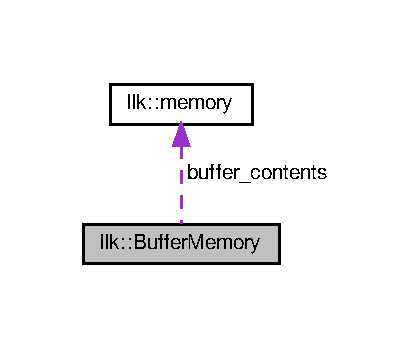
\includegraphics[width=198pt]{structllk_1_1BufferMemory__coll__graph}
\end{center}
\end{figure}
\subsection*{Public Attributes}
\begin{DoxyCompactItemize}
\item 
boost\+::optional$<$ \hyperlink{classllk_1_1memory}{memory} $>$ \hyperlink{structllk_1_1BufferMemory_a1d36015b797463afc7527cbb22f5a31e}{header}
\item 
\hyperlink{classllk_1_1memory}{memory} \hyperlink{structllk_1_1BufferMemory_a0603bea5cb9a94a719d79d49ffe0969c}{buffer\+\_\+contents}
\end{DoxyCompactItemize}


\subsection{Member Data Documentation}
\mbox{\Hypertarget{structllk_1_1BufferMemory_a0603bea5cb9a94a719d79d49ffe0969c}\label{structllk_1_1BufferMemory_a0603bea5cb9a94a719d79d49ffe0969c}} 
\index{llk\+::\+Buffer\+Memory@{llk\+::\+Buffer\+Memory}!buffer\+\_\+contents@{buffer\+\_\+contents}}
\index{buffer\+\_\+contents@{buffer\+\_\+contents}!llk\+::\+Buffer\+Memory@{llk\+::\+Buffer\+Memory}}
\subsubsection{\texorpdfstring{buffer\+\_\+contents}{buffer\_contents}}
{\footnotesize\ttfamily \hyperlink{classllk_1_1memory}{memory} llk\+::\+Buffer\+Memory\+::buffer\+\_\+contents}

\mbox{\Hypertarget{structllk_1_1BufferMemory_a1d36015b797463afc7527cbb22f5a31e}\label{structllk_1_1BufferMemory_a1d36015b797463afc7527cbb22f5a31e}} 
\index{llk\+::\+Buffer\+Memory@{llk\+::\+Buffer\+Memory}!header@{header}}
\index{header@{header}!llk\+::\+Buffer\+Memory@{llk\+::\+Buffer\+Memory}}
\subsubsection{\texorpdfstring{header}{header}}
{\footnotesize\ttfamily boost\+::optional$<$\hyperlink{classllk_1_1memory}{memory}$>$ llk\+::\+Buffer\+Memory\+::header}



The documentation for this struct was generated from the following file\+:\begin{DoxyCompactItemize}
\item 
inc/\hyperlink{llk__memory_8h}{llk\+\_\+memory.\+h}\end{DoxyCompactItemize}

\hypertarget{structllk_1_1CoreDescriptor}{}\section{llk\+:\+:Core\+Descriptor Struct Reference}
\label{structllk_1_1CoreDescriptor}\index{llk\+::\+Core\+Descriptor@{llk\+::\+Core\+Descriptor}}


Soc\+Node\+Descriptor contains information regarding the Node/\+Core.  




{\ttfamily \#include $<$llk\+\_\+soc\+\_\+descriptor.\+h$>$}



Collaboration diagram for llk\+:\+:Core\+Descriptor\+:\nopagebreak
\begin{figure}[H]
\begin{center}
\leavevmode
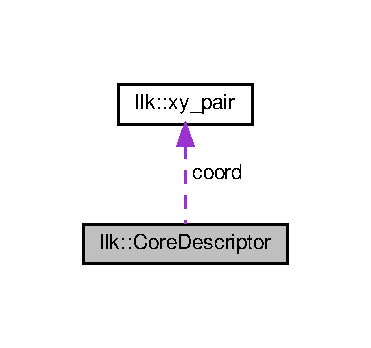
\includegraphics[width=178pt]{structllk_1_1CoreDescriptor__coll__graph}
\end{center}
\end{figure}
\subsection*{Public Attributes}
\begin{DoxyCompactItemize}
\item 
\hyperlink{structllk_1_1xy__pair}{llk\+::xy\+\_\+pair} \hyperlink{structllk_1_1CoreDescriptor_aa32a249d368698c0dd0faa96a483f073}{coord} = \hyperlink{structllk_1_1xy__pair}{llk\+::xy\+\_\+pair}(0, 0)
\item 
\hyperlink{namespacellk_ad3e730e596589754342a98abd7021ed4}{Core\+Type} \hyperlink{structllk_1_1CoreDescriptor_a7191de431135e380831699043a13b26d}{type}
\item 
std\+::size\+\_\+t \hyperlink{structllk_1_1CoreDescriptor_a4e20170592b4452b98402bafb139e89d}{l1\+\_\+size} = 0
\item 
std\+::size\+\_\+t \hyperlink{structllk_1_1CoreDescriptor_aafc94079c5c809b77dece07d39d48666}{dram\+\_\+size\+\_\+per\+\_\+core} = 0
\end{DoxyCompactItemize}


\subsection{Detailed Description}
Soc\+Node\+Descriptor contains information regarding the Node/\+Core. 

Should only contain relevant configuration for S\+OC 

\subsection{Member Data Documentation}
\mbox{\Hypertarget{structllk_1_1CoreDescriptor_aa32a249d368698c0dd0faa96a483f073}\label{structllk_1_1CoreDescriptor_aa32a249d368698c0dd0faa96a483f073}} 
\index{llk\+::\+Core\+Descriptor@{llk\+::\+Core\+Descriptor}!coord@{coord}}
\index{coord@{coord}!llk\+::\+Core\+Descriptor@{llk\+::\+Core\+Descriptor}}
\subsubsection{\texorpdfstring{coord}{coord}}
{\footnotesize\ttfamily \hyperlink{structllk_1_1xy__pair}{llk\+::xy\+\_\+pair} llk\+::\+Core\+Descriptor\+::coord = \hyperlink{structllk_1_1xy__pair}{llk\+::xy\+\_\+pair}(0, 0)}

\mbox{\Hypertarget{structllk_1_1CoreDescriptor_aafc94079c5c809b77dece07d39d48666}\label{structllk_1_1CoreDescriptor_aafc94079c5c809b77dece07d39d48666}} 
\index{llk\+::\+Core\+Descriptor@{llk\+::\+Core\+Descriptor}!dram\+\_\+size\+\_\+per\+\_\+core@{dram\+\_\+size\+\_\+per\+\_\+core}}
\index{dram\+\_\+size\+\_\+per\+\_\+core@{dram\+\_\+size\+\_\+per\+\_\+core}!llk\+::\+Core\+Descriptor@{llk\+::\+Core\+Descriptor}}
\subsubsection{\texorpdfstring{dram\+\_\+size\+\_\+per\+\_\+core}{dram\_size\_per\_core}}
{\footnotesize\ttfamily std\+::size\+\_\+t llk\+::\+Core\+Descriptor\+::dram\+\_\+size\+\_\+per\+\_\+core = 0}

\mbox{\Hypertarget{structllk_1_1CoreDescriptor_a4e20170592b4452b98402bafb139e89d}\label{structllk_1_1CoreDescriptor_a4e20170592b4452b98402bafb139e89d}} 
\index{llk\+::\+Core\+Descriptor@{llk\+::\+Core\+Descriptor}!l1\+\_\+size@{l1\+\_\+size}}
\index{l1\+\_\+size@{l1\+\_\+size}!llk\+::\+Core\+Descriptor@{llk\+::\+Core\+Descriptor}}
\subsubsection{\texorpdfstring{l1\+\_\+size}{l1\_size}}
{\footnotesize\ttfamily std\+::size\+\_\+t llk\+::\+Core\+Descriptor\+::l1\+\_\+size = 0}

\mbox{\Hypertarget{structllk_1_1CoreDescriptor_a7191de431135e380831699043a13b26d}\label{structllk_1_1CoreDescriptor_a7191de431135e380831699043a13b26d}} 
\index{llk\+::\+Core\+Descriptor@{llk\+::\+Core\+Descriptor}!type@{type}}
\index{type@{type}!llk\+::\+Core\+Descriptor@{llk\+::\+Core\+Descriptor}}
\subsubsection{\texorpdfstring{type}{type}}
{\footnotesize\ttfamily \hyperlink{namespacellk_ad3e730e596589754342a98abd7021ed4}{Core\+Type} llk\+::\+Core\+Descriptor\+::type}



The documentation for this struct was generated from the following file\+:\begin{DoxyCompactItemize}
\item 
inc/\hyperlink{llk__soc__descriptor_8h}{llk\+\_\+soc\+\_\+descriptor.\+h}\end{DoxyCompactItemize}

\hypertarget{classllk_1_1Device}{}\section{llk\+:\+:Device Class Reference}
\label{classllk_1_1Device}\index{llk\+::\+Device@{llk\+::\+Device}}


\hyperlink{classllk_1_1Device}{Device} A\+PI in a wrapper class.  




{\ttfamily \#include $<$llk\+\_\+device.\+h$>$}



Collaboration diagram for llk\+:\+:Device\+:\nopagebreak
\begin{figure}[H]
\begin{center}
\leavevmode
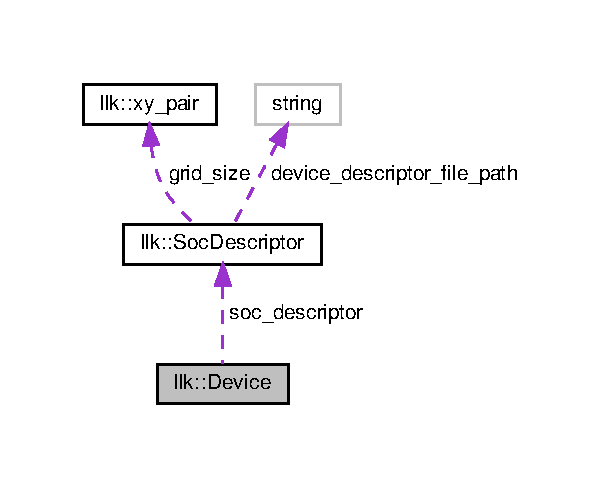
\includegraphics[width=289pt]{classllk_1_1Device__coll__graph}
\end{center}
\end{figure}
\subsection*{Public Member Functions}
\begin{DoxyCompactItemize}
\item 
void \hyperlink{classllk_1_1Device_a4be879d10344eab03473e53e41cc14b8}{start} (std\+::string root, std\+::string device\+\_\+descriptor\+\_\+filename, std\+::vector$<$ std\+::string $>$ plusargs, std\+::vector$<$ std\+::string $>$ dump\+\_\+cores, std\+::string overlay\+\_\+graph=\char`\"{}\char`\"{})
\begin{DoxyCompactList}\small\item\em Starts device. \end{DoxyCompactList}\item 
void \hyperlink{classllk_1_1Device_a8e68d577fd5c160567e31dc0518bd6e9}{setup\+\_\+kernels} (std\+::string root, std\+::unordered\+\_\+map$<$ \hyperlink{structllk_1_1xy__pair}{llk\+::xy\+\_\+pair}, std\+::vector$<$ std\+::vector$<$ std\+::string $>$$>$$>$ \&kernels\+\_\+used, std\+::string test\+\_\+name, bool hlkc\+\_\+test=false)
\begin{DoxyCompactList}\small\item\em Sets up test information (ckernels images etc) \end{DoxyCompactList}\item 
void \hyperlink{classllk_1_1Device_a15b42f2d1a734de7cd14b33a93bb87e2}{generate\+\_\+overlay\+\_\+blob} (std\+::string root, std\+::map$<$ std\+::string, std\+::string $>$ blob\+\_\+args)
\begin{DoxyCompactList}\small\item\em Builds overlay blob hex files. \end{DoxyCompactList}\item 
bool \hyperlink{classllk_1_1Device_a70a42e9710b3c971685f38733852e90e}{run} ()
\begin{DoxyCompactList}\small\item\em Runs simulation. \end{DoxyCompactList}\item 
bool \hyperlink{classllk_1_1Device_a6f6a546079d7c976635093e85ef6d348}{stop} ()
\begin{DoxyCompactList}\small\item\em Stops and teardowns device. \end{DoxyCompactList}\item 
void \hyperlink{classllk_1_1Device_ad0bcc94a905851a6c78bb84873ff780d}{write\+\_\+register} (uint32\+\_\+t \&value, \hyperlink{structllk_1_1xy__pair}{llk\+::xy\+\_\+pair} target, std\+::int32\+\_\+t address)
\begin{DoxyCompactList}\small\item\em write vector to specific core -- address is byte address \end{DoxyCompactList}\item 
void \hyperlink{classllk_1_1Device_a6960399d0aa112fc17d743423e7fc9f9}{read\+\_\+register} (uint32\+\_\+t \&value, \hyperlink{structllk_1_1xy__pair}{llk\+::xy\+\_\+pair} target, std\+::int32\+\_\+t address)
\begin{DoxyCompactList}\small\item\em read vector from specific core -- address is byte address \end{DoxyCompactList}\item 
void \hyperlink{classllk_1_1Device_a5704d979e68f372b6490ddf52e6bbff4}{write\+\_\+vector} (std\+::vector$<$ std\+::uint32\+\_\+t $>$ \&mem\+\_\+vector, \hyperlink{structllk_1_1xy__pair}{llk\+::xy\+\_\+pair} target, std\+::int32\+\_\+t address)
\begin{DoxyCompactList}\small\item\em write vector to specific core -- address is byte address \end{DoxyCompactList}\item 
void \hyperlink{classllk_1_1Device_a1e742a4ebe3f474152878830c5e12388}{read\+\_\+vector} (std\+::vector$<$ std\+::uint32\+\_\+t $>$ \&mem\+\_\+vector, \hyperlink{structllk_1_1xy__pair}{llk\+::xy\+\_\+pair} target, std\+::int32\+\_\+t address, std\+::int32\+\_\+t size\+\_\+in\+\_\+bytes)
\begin{DoxyCompactList}\small\item\em read vector from specific core -- address is byte address \end{DoxyCompactList}\item 
void \hyperlink{classllk_1_1Device_a636a9edf251c886873b8cd2140329730}{write\+\_\+tensor} (\hyperlink{classllk_1_1Tensor}{llk\+::\+Tensor} \&tensor, \hyperlink{structllk_1_1xy__pair}{llk\+::xy\+\_\+pair} target, std\+::int32\+\_\+t address, \hyperlink{structllk_1_1xy__pair}{llk\+::xy\+\_\+pair} num\+\_\+blocks=\hyperlink{structllk_1_1xy__pair}{llk\+::xy\+\_\+pair}(1, 1))
\begin{DoxyCompactList}\small\item\em write tensor to specific core -- address is byte address \end{DoxyCompactList}\item 
void \hyperlink{classllk_1_1Device_ac399c05757459303f9d3ae64c52359da}{read\+\_\+tensor} (\hyperlink{classllk_1_1Tensor}{llk\+::\+Tensor} \&tensor, \hyperlink{structllk_1_1xy__pair}{llk\+::xy\+\_\+pair} target, std\+::int32\+\_\+t address)
\begin{DoxyCompactList}\small\item\em read tensor from specific core \end{DoxyCompactList}\item 
bool \hyperlink{classllk_1_1Device_a860d5ea1706c7fc693ed2f7da2de9874}{wait\+\_\+completion} (std\+::uint32\+\_\+t W\+A\+I\+T\+\_\+\+N\+U\+M\+\_\+\+R\+I\+S\+CS=5)
\begin{DoxyCompactList}\small\item\em Wait for completion status/signal from device. \end{DoxyCompactList}\item 
bool \hyperlink{classllk_1_1Device_a9086600f456bd20655b2bd74b8d10017}{test\+\_\+write\+\_\+read} (\hyperlink{structllk_1_1xy__pair}{llk\+::xy\+\_\+pair} target)
\begin{DoxyCompactList}\small\item\em Simple test of communication to device/target. true if it passes. \end{DoxyCompactList}\end{DoxyCompactItemize}
\subsection*{Public Attributes}
\begin{DoxyCompactItemize}
\item 
\hyperlink{structllk_1_1SocDescriptor}{llk\+::\+Soc\+Descriptor} \hyperlink{classllk_1_1Device_a00b7609fbc13977bb9ea6522c53feeb4}{soc\+\_\+descriptor}
\end{DoxyCompactItemize}


\subsection{Detailed Description}
\hyperlink{classllk_1_1Device}{Device} A\+PI in a wrapper class. 

\subsection{Member Function Documentation}
\mbox{\Hypertarget{classllk_1_1Device_a15b42f2d1a734de7cd14b33a93bb87e2}\label{classllk_1_1Device_a15b42f2d1a734de7cd14b33a93bb87e2}} 
\index{llk\+::\+Device@{llk\+::\+Device}!generate\+\_\+overlay\+\_\+blob@{generate\+\_\+overlay\+\_\+blob}}
\index{generate\+\_\+overlay\+\_\+blob@{generate\+\_\+overlay\+\_\+blob}!llk\+::\+Device@{llk\+::\+Device}}
\subsubsection{\texorpdfstring{generate\+\_\+overlay\+\_\+blob()}{generate\_overlay\_blob()}}
{\footnotesize\ttfamily void llk\+::\+Device\+::generate\+\_\+overlay\+\_\+blob (\begin{DoxyParamCaption}\item[{std\+::string}]{root,  }\item[{std\+::map$<$ std\+::string, std\+::string $>$}]{blob\+\_\+args }\end{DoxyParamCaption})}



Builds overlay blob hex files. 

\mbox{\Hypertarget{classllk_1_1Device_a6960399d0aa112fc17d743423e7fc9f9}\label{classllk_1_1Device_a6960399d0aa112fc17d743423e7fc9f9}} 
\index{llk\+::\+Device@{llk\+::\+Device}!read\+\_\+register@{read\+\_\+register}}
\index{read\+\_\+register@{read\+\_\+register}!llk\+::\+Device@{llk\+::\+Device}}
\subsubsection{\texorpdfstring{read\+\_\+register()}{read\_register()}}
{\footnotesize\ttfamily void llk\+::\+Device\+::read\+\_\+register (\begin{DoxyParamCaption}\item[{uint32\+\_\+t \&}]{value,  }\item[{\hyperlink{structllk_1_1xy__pair}{llk\+::xy\+\_\+pair}}]{target,  }\item[{std\+::int32\+\_\+t}]{address }\end{DoxyParamCaption})}



read vector from specific core -- address is byte address 


\begin{DoxyParams}{Parameters}
{\em mem\+\_\+vector} & is the vector to read \\
\hline
{\em target} & is xy coordinate that is the target of the read or write \\
\hline
{\em address} & is register byte address \\
\hline
\end{DoxyParams}
\mbox{\Hypertarget{classllk_1_1Device_ac399c05757459303f9d3ae64c52359da}\label{classllk_1_1Device_ac399c05757459303f9d3ae64c52359da}} 
\index{llk\+::\+Device@{llk\+::\+Device}!read\+\_\+tensor@{read\+\_\+tensor}}
\index{read\+\_\+tensor@{read\+\_\+tensor}!llk\+::\+Device@{llk\+::\+Device}}
\subsubsection{\texorpdfstring{read\+\_\+tensor()}{read\_tensor()}}
{\footnotesize\ttfamily void llk\+::\+Device\+::read\+\_\+tensor (\begin{DoxyParamCaption}\item[{\hyperlink{classllk_1_1Tensor}{llk\+::\+Tensor} \&}]{tensor,  }\item[{\hyperlink{structllk_1_1xy__pair}{llk\+::xy\+\_\+pair}}]{target,  }\item[{std\+::int32\+\_\+t}]{address }\end{DoxyParamCaption})}



read tensor from specific core 


\begin{DoxyParams}{Parameters}
{\em tensor} & is the destination tensor to fill. Dimension and format must be initialized correctly! \\
\hline
{\em target} & is xy coordinate that is the target of the read or write \\
\hline
{\em address} & is byte address \\
\hline
{\em dims} & is tensor dimensions \\
\hline
\end{DoxyParams}
\mbox{\Hypertarget{classllk_1_1Device_a1e742a4ebe3f474152878830c5e12388}\label{classllk_1_1Device_a1e742a4ebe3f474152878830c5e12388}} 
\index{llk\+::\+Device@{llk\+::\+Device}!read\+\_\+vector@{read\+\_\+vector}}
\index{read\+\_\+vector@{read\+\_\+vector}!llk\+::\+Device@{llk\+::\+Device}}
\subsubsection{\texorpdfstring{read\+\_\+vector()}{read\_vector()}}
{\footnotesize\ttfamily void llk\+::\+Device\+::read\+\_\+vector (\begin{DoxyParamCaption}\item[{std\+::vector$<$ std\+::uint32\+\_\+t $>$ \&}]{mem\+\_\+vector,  }\item[{\hyperlink{structllk_1_1xy__pair}{llk\+::xy\+\_\+pair}}]{target,  }\item[{std\+::int32\+\_\+t}]{address,  }\item[{std\+::int32\+\_\+t}]{size\+\_\+in\+\_\+bytes }\end{DoxyParamCaption})}



read vector from specific core -- address is byte address 


\begin{DoxyParams}{Parameters}
{\em mem\+\_\+vector} & is the vector to read \\
\hline
{\em target} & is xy coordinate that is the target of the read or write \\
\hline
{\em address} & is byte address \\
\hline
{\em size\+\_\+in\+\_\+bytes} & is number of bytes to read \\
\hline
\end{DoxyParams}
\mbox{\Hypertarget{classllk_1_1Device_a70a42e9710b3c971685f38733852e90e}\label{classllk_1_1Device_a70a42e9710b3c971685f38733852e90e}} 
\index{llk\+::\+Device@{llk\+::\+Device}!run@{run}}
\index{run@{run}!llk\+::\+Device@{llk\+::\+Device}}
\subsubsection{\texorpdfstring{run()}{run()}}
{\footnotesize\ttfamily bool llk\+::\+Device\+::run (\begin{DoxyParamCaption}{ }\end{DoxyParamCaption})}



Runs simulation. 

\mbox{\Hypertarget{classllk_1_1Device_a8e68d577fd5c160567e31dc0518bd6e9}\label{classllk_1_1Device_a8e68d577fd5c160567e31dc0518bd6e9}} 
\index{llk\+::\+Device@{llk\+::\+Device}!setup\+\_\+kernels@{setup\+\_\+kernels}}
\index{setup\+\_\+kernels@{setup\+\_\+kernels}!llk\+::\+Device@{llk\+::\+Device}}
\subsubsection{\texorpdfstring{setup\+\_\+kernels()}{setup\_kernels()}}
{\footnotesize\ttfamily void llk\+::\+Device\+::setup\+\_\+kernels (\begin{DoxyParamCaption}\item[{std\+::string}]{root,  }\item[{std\+::unordered\+\_\+map$<$ \hyperlink{structllk_1_1xy__pair}{llk\+::xy\+\_\+pair}, std\+::vector$<$ std\+::vector$<$ std\+::string $>$$>$$>$ \&}]{kernels\+\_\+used,  }\item[{std\+::string}]{test\+\_\+name,  }\item[{bool}]{hlkc\+\_\+test = {\ttfamily false} }\end{DoxyParamCaption})}



Sets up test information (ckernels images etc) 

\mbox{\Hypertarget{classllk_1_1Device_a4be879d10344eab03473e53e41cc14b8}\label{classllk_1_1Device_a4be879d10344eab03473e53e41cc14b8}} 
\index{llk\+::\+Device@{llk\+::\+Device}!start@{start}}
\index{start@{start}!llk\+::\+Device@{llk\+::\+Device}}
\subsubsection{\texorpdfstring{start()}{start()}}
{\footnotesize\ttfamily void llk\+::\+Device\+::start (\begin{DoxyParamCaption}\item[{std\+::string}]{root,  }\item[{std\+::string}]{device\+\_\+descriptor\+\_\+filename,  }\item[{std\+::vector$<$ std\+::string $>$}]{plusargs,  }\item[{std\+::vector$<$ std\+::string $>$}]{dump\+\_\+cores,  }\item[{std\+::string}]{overlay\+\_\+graph = {\ttfamily \char`\"{}\char`\"{}} }\end{DoxyParamCaption})}



Starts device. 


\begin{DoxyParams}{Parameters}
{\em device} & Reference to device object that is to be started \\
\hline
{\em root} & root folder (git root) \\
\hline
{\em dump\+\_\+cores} & vector of cores to dump in simulation \\
\hline
\end{DoxyParams}
\mbox{\Hypertarget{classllk_1_1Device_a6f6a546079d7c976635093e85ef6d348}\label{classllk_1_1Device_a6f6a546079d7c976635093e85ef6d348}} 
\index{llk\+::\+Device@{llk\+::\+Device}!stop@{stop}}
\index{stop@{stop}!llk\+::\+Device@{llk\+::\+Device}}
\subsubsection{\texorpdfstring{stop()}{stop()}}
{\footnotesize\ttfamily bool llk\+::\+Device\+::stop (\begin{DoxyParamCaption}{ }\end{DoxyParamCaption})}



Stops and teardowns device. 

\mbox{\Hypertarget{classllk_1_1Device_a9086600f456bd20655b2bd74b8d10017}\label{classllk_1_1Device_a9086600f456bd20655b2bd74b8d10017}} 
\index{llk\+::\+Device@{llk\+::\+Device}!test\+\_\+write\+\_\+read@{test\+\_\+write\+\_\+read}}
\index{test\+\_\+write\+\_\+read@{test\+\_\+write\+\_\+read}!llk\+::\+Device@{llk\+::\+Device}}
\subsubsection{\texorpdfstring{test\+\_\+write\+\_\+read()}{test\_write\_read()}}
{\footnotesize\ttfamily bool llk\+::\+Device\+::test\+\_\+write\+\_\+read (\begin{DoxyParamCaption}\item[{\hyperlink{structllk_1_1xy__pair}{llk\+::xy\+\_\+pair}}]{target }\end{DoxyParamCaption})}



Simple test of communication to device/target. true if it passes. 

\mbox{\Hypertarget{classllk_1_1Device_a860d5ea1706c7fc693ed2f7da2de9874}\label{classllk_1_1Device_a860d5ea1706c7fc693ed2f7da2de9874}} 
\index{llk\+::\+Device@{llk\+::\+Device}!wait\+\_\+completion@{wait\+\_\+completion}}
\index{wait\+\_\+completion@{wait\+\_\+completion}!llk\+::\+Device@{llk\+::\+Device}}
\subsubsection{\texorpdfstring{wait\+\_\+completion()}{wait\_completion()}}
{\footnotesize\ttfamily bool llk\+::\+Device\+::wait\+\_\+completion (\begin{DoxyParamCaption}\item[{std\+::uint32\+\_\+t}]{W\+A\+I\+T\+\_\+\+N\+U\+M\+\_\+\+R\+I\+S\+CS = {\ttfamily 5} }\end{DoxyParamCaption})}



Wait for completion status/signal from device. 

\mbox{\Hypertarget{classllk_1_1Device_ad0bcc94a905851a6c78bb84873ff780d}\label{classllk_1_1Device_ad0bcc94a905851a6c78bb84873ff780d}} 
\index{llk\+::\+Device@{llk\+::\+Device}!write\+\_\+register@{write\+\_\+register}}
\index{write\+\_\+register@{write\+\_\+register}!llk\+::\+Device@{llk\+::\+Device}}
\subsubsection{\texorpdfstring{write\+\_\+register()}{write\_register()}}
{\footnotesize\ttfamily void llk\+::\+Device\+::write\+\_\+register (\begin{DoxyParamCaption}\item[{uint32\+\_\+t \&}]{value,  }\item[{\hyperlink{structllk_1_1xy__pair}{llk\+::xy\+\_\+pair}}]{target,  }\item[{std\+::int32\+\_\+t}]{address }\end{DoxyParamCaption})}



write vector to specific core -- address is byte address 


\begin{DoxyParams}{Parameters}
{\em mem\+\_\+vector} & is the vector to write. \\
\hline
{\em target} & is xy coordinate that is the target of the read or write \\
\hline
{\em address} & is register byte address \\
\hline
\end{DoxyParams}
\mbox{\Hypertarget{classllk_1_1Device_a636a9edf251c886873b8cd2140329730}\label{classllk_1_1Device_a636a9edf251c886873b8cd2140329730}} 
\index{llk\+::\+Device@{llk\+::\+Device}!write\+\_\+tensor@{write\+\_\+tensor}}
\index{write\+\_\+tensor@{write\+\_\+tensor}!llk\+::\+Device@{llk\+::\+Device}}
\subsubsection{\texorpdfstring{write\+\_\+tensor()}{write\_tensor()}}
{\footnotesize\ttfamily void llk\+::\+Device\+::write\+\_\+tensor (\begin{DoxyParamCaption}\item[{\hyperlink{classllk_1_1Tensor}{llk\+::\+Tensor} \&}]{tensor,  }\item[{\hyperlink{structllk_1_1xy__pair}{llk\+::xy\+\_\+pair}}]{target,  }\item[{std\+::int32\+\_\+t}]{address,  }\item[{\hyperlink{structllk_1_1xy__pair}{llk\+::xy\+\_\+pair}}]{num\+\_\+blocks = {\ttfamily \hyperlink{structllk_1_1xy__pair}{llk\+::xy\+\_\+pair}(1,~1)} }\end{DoxyParamCaption})}



write tensor to specific core -- address is byte address 


\begin{DoxyParams}{Parameters}
{\em tensor} & is the tensor to write. \\
\hline
{\em target} & is xy coordinate that is the target of the read or write \\
\hline
{\em address} & is byte address \\
\hline
{\em num\+\_\+blocks} & is how many blocks in x or y dims the tensor needs to be split. Default of 1,1 means no splitting \\
\hline
\end{DoxyParams}
\mbox{\Hypertarget{classllk_1_1Device_a5704d979e68f372b6490ddf52e6bbff4}\label{classllk_1_1Device_a5704d979e68f372b6490ddf52e6bbff4}} 
\index{llk\+::\+Device@{llk\+::\+Device}!write\+\_\+vector@{write\+\_\+vector}}
\index{write\+\_\+vector@{write\+\_\+vector}!llk\+::\+Device@{llk\+::\+Device}}
\subsubsection{\texorpdfstring{write\+\_\+vector()}{write\_vector()}}
{\footnotesize\ttfamily void llk\+::\+Device\+::write\+\_\+vector (\begin{DoxyParamCaption}\item[{std\+::vector$<$ std\+::uint32\+\_\+t $>$ \&}]{mem\+\_\+vector,  }\item[{\hyperlink{structllk_1_1xy__pair}{llk\+::xy\+\_\+pair}}]{target,  }\item[{std\+::int32\+\_\+t}]{address }\end{DoxyParamCaption})}



write vector to specific core -- address is byte address 


\begin{DoxyParams}{Parameters}
{\em mem\+\_\+vector} & is the vector to write. \\
\hline
{\em target} & is xy coordinate that is the target of the read or write \\
\hline
{\em address} & is byte address \\
\hline
\end{DoxyParams}


\subsection{Member Data Documentation}
\mbox{\Hypertarget{classllk_1_1Device_a00b7609fbc13977bb9ea6522c53feeb4}\label{classllk_1_1Device_a00b7609fbc13977bb9ea6522c53feeb4}} 
\index{llk\+::\+Device@{llk\+::\+Device}!soc\+\_\+descriptor@{soc\+\_\+descriptor}}
\index{soc\+\_\+descriptor@{soc\+\_\+descriptor}!llk\+::\+Device@{llk\+::\+Device}}
\subsubsection{\texorpdfstring{soc\+\_\+descriptor}{soc\_descriptor}}
{\footnotesize\ttfamily \hyperlink{structllk_1_1SocDescriptor}{llk\+::\+Soc\+Descriptor} llk\+::\+Device\+::soc\+\_\+descriptor}



The documentation for this class was generated from the following files\+:\begin{DoxyCompactItemize}
\item 
inc/\hyperlink{llk__device_8h}{llk\+\_\+device.\+h}\item 
src/\hyperlink{llk__device_8cpp}{llk\+\_\+device.\+cpp}\end{DoxyCompactItemize}

\hypertarget{classllk_1_1discontiguous__hex__file__writer}{}\section{llk\+:\+:discontiguous\+\_\+hex\+\_\+file\+\_\+writer Class Reference}
\label{classllk_1_1discontiguous__hex__file__writer}\index{llk\+::discontiguous\+\_\+hex\+\_\+file\+\_\+writer@{llk\+::discontiguous\+\_\+hex\+\_\+file\+\_\+writer}}


{\ttfamily \#include $<$llk\+\_\+hexfile.\+h$>$}

\subsection*{Public Member Functions}
\begin{DoxyCompactItemize}
\item 
\hyperlink{classllk_1_1discontiguous__hex__file__writer_a90e03c9ab8efd0c571fd53db27bcf386}{discontiguous\+\_\+hex\+\_\+file\+\_\+writer} (std\+::ostream \&output)
\item 
void \hyperlink{classllk_1_1discontiguous__hex__file__writer_a4dc35f2a9382c453d050d3e0ef8e1898}{add} (\hyperlink{classllk_1_1memory_ae7a4b897aa999f22e250dc8e4d773dec}{memory\+::address\+\_\+t} address, \hyperlink{classllk_1_1memory_a432a6c0ae1bcb9c44d79cfa1a239419c}{memory\+::word\+\_\+t} value)
\item 
{\footnotesize template$<$class Iterator $>$ }\\void \hyperlink{classllk_1_1discontiguous__hex__file__writer_abadd72236ae15b74466c96f058290657}{add} (\hyperlink{classllk_1_1memory_ae7a4b897aa999f22e250dc8e4d773dec}{memory\+::address\+\_\+t} start\+\_\+address, Iterator first, Iterator last)
\item 
void \hyperlink{classllk_1_1discontiguous__hex__file__writer_a7821a63136b422abdc17b8d9efdc1cf9}{end} ()
\end{DoxyCompactItemize}


\subsection{Constructor \& Destructor Documentation}
\mbox{\Hypertarget{classllk_1_1discontiguous__hex__file__writer_a90e03c9ab8efd0c571fd53db27bcf386}\label{classllk_1_1discontiguous__hex__file__writer_a90e03c9ab8efd0c571fd53db27bcf386}} 
\index{llk\+::discontiguous\+\_\+hex\+\_\+file\+\_\+writer@{llk\+::discontiguous\+\_\+hex\+\_\+file\+\_\+writer}!discontiguous\+\_\+hex\+\_\+file\+\_\+writer@{discontiguous\+\_\+hex\+\_\+file\+\_\+writer}}
\index{discontiguous\+\_\+hex\+\_\+file\+\_\+writer@{discontiguous\+\_\+hex\+\_\+file\+\_\+writer}!llk\+::discontiguous\+\_\+hex\+\_\+file\+\_\+writer@{llk\+::discontiguous\+\_\+hex\+\_\+file\+\_\+writer}}
\subsubsection{\texorpdfstring{discontiguous\+\_\+hex\+\_\+file\+\_\+writer()}{discontiguous\_hex\_file\_writer()}}
{\footnotesize\ttfamily llk\+::discontiguous\+\_\+hex\+\_\+file\+\_\+writer\+::discontiguous\+\_\+hex\+\_\+file\+\_\+writer (\begin{DoxyParamCaption}\item[{std\+::ostream \&}]{output }\end{DoxyParamCaption})\hspace{0.3cm}{\ttfamily [explicit]}}



\subsection{Member Function Documentation}
\mbox{\Hypertarget{classllk_1_1discontiguous__hex__file__writer_a4dc35f2a9382c453d050d3e0ef8e1898}\label{classllk_1_1discontiguous__hex__file__writer_a4dc35f2a9382c453d050d3e0ef8e1898}} 
\index{llk\+::discontiguous\+\_\+hex\+\_\+file\+\_\+writer@{llk\+::discontiguous\+\_\+hex\+\_\+file\+\_\+writer}!add@{add}}
\index{add@{add}!llk\+::discontiguous\+\_\+hex\+\_\+file\+\_\+writer@{llk\+::discontiguous\+\_\+hex\+\_\+file\+\_\+writer}}
\subsubsection{\texorpdfstring{add()}{add()}\hspace{0.1cm}{\footnotesize\ttfamily [1/2]}}
{\footnotesize\ttfamily void llk\+::discontiguous\+\_\+hex\+\_\+file\+\_\+writer\+::add (\begin{DoxyParamCaption}\item[{\hyperlink{classllk_1_1memory_ae7a4b897aa999f22e250dc8e4d773dec}{memory\+::address\+\_\+t}}]{address,  }\item[{\hyperlink{classllk_1_1memory_a432a6c0ae1bcb9c44d79cfa1a239419c}{memory\+::word\+\_\+t}}]{value }\end{DoxyParamCaption})}

\mbox{\Hypertarget{classllk_1_1discontiguous__hex__file__writer_abadd72236ae15b74466c96f058290657}\label{classllk_1_1discontiguous__hex__file__writer_abadd72236ae15b74466c96f058290657}} 
\index{llk\+::discontiguous\+\_\+hex\+\_\+file\+\_\+writer@{llk\+::discontiguous\+\_\+hex\+\_\+file\+\_\+writer}!add@{add}}
\index{add@{add}!llk\+::discontiguous\+\_\+hex\+\_\+file\+\_\+writer@{llk\+::discontiguous\+\_\+hex\+\_\+file\+\_\+writer}}
\subsubsection{\texorpdfstring{add()}{add()}\hspace{0.1cm}{\footnotesize\ttfamily [2/2]}}
{\footnotesize\ttfamily template$<$class Iterator $>$ \\
void llk\+::discontiguous\+\_\+hex\+\_\+file\+\_\+writer\+::add (\begin{DoxyParamCaption}\item[{\hyperlink{classllk_1_1memory_ae7a4b897aa999f22e250dc8e4d773dec}{memory\+::address\+\_\+t}}]{start\+\_\+address,  }\item[{Iterator}]{first,  }\item[{Iterator}]{last }\end{DoxyParamCaption})\hspace{0.3cm}{\ttfamily [inline]}}

\mbox{\Hypertarget{classllk_1_1discontiguous__hex__file__writer_a7821a63136b422abdc17b8d9efdc1cf9}\label{classllk_1_1discontiguous__hex__file__writer_a7821a63136b422abdc17b8d9efdc1cf9}} 
\index{llk\+::discontiguous\+\_\+hex\+\_\+file\+\_\+writer@{llk\+::discontiguous\+\_\+hex\+\_\+file\+\_\+writer}!end@{end}}
\index{end@{end}!llk\+::discontiguous\+\_\+hex\+\_\+file\+\_\+writer@{llk\+::discontiguous\+\_\+hex\+\_\+file\+\_\+writer}}
\subsubsection{\texorpdfstring{end()}{end()}}
{\footnotesize\ttfamily void llk\+::discontiguous\+\_\+hex\+\_\+file\+\_\+writer\+::end (\begin{DoxyParamCaption}{ }\end{DoxyParamCaption})\hspace{0.3cm}{\ttfamily [inline]}}



The documentation for this class was generated from the following files\+:\begin{DoxyCompactItemize}
\item 
inc/\hyperlink{llk__hexfile_8h}{llk\+\_\+hexfile.\+h}\item 
src/\hyperlink{llk__hexfile_8cpp}{llk\+\_\+hexfile.\+cpp}\end{DoxyCompactItemize}

\hypertarget{structstd_1_1hash_3_01llk_1_1xy__pair_01_4}{}\section{std\+:\+:hash$<$ llk\+:\+:xy\+\_\+pair $>$ Struct Template Reference}
\label{structstd_1_1hash_3_01llk_1_1xy__pair_01_4}\index{std\+::hash$<$ llk\+::xy\+\_\+pair $>$@{std\+::hash$<$ llk\+::xy\+\_\+pair $>$}}


{\ttfamily \#include $<$llk\+\_\+xy\+\_\+pair.\+h$>$}

\subsection*{Public Member Functions}
\begin{DoxyCompactItemize}
\item 
std\+::size\+\_\+t \hyperlink{structstd_1_1hash_3_01llk_1_1xy__pair_01_4_ae4dec4648fbc30a1d328be77b17f9b34}{operator()} (\hyperlink{structllk_1_1xy__pair}{llk\+::xy\+\_\+pair} const \&o) const
\end{DoxyCompactItemize}


\subsection{Member Function Documentation}
\mbox{\Hypertarget{structstd_1_1hash_3_01llk_1_1xy__pair_01_4_ae4dec4648fbc30a1d328be77b17f9b34}\label{structstd_1_1hash_3_01llk_1_1xy__pair_01_4_ae4dec4648fbc30a1d328be77b17f9b34}} 
\index{std\+::hash$<$ llk\+::xy\+\_\+pair $>$@{std\+::hash$<$ llk\+::xy\+\_\+pair $>$}!operator()@{operator()}}
\index{operator()@{operator()}!std\+::hash$<$ llk\+::xy\+\_\+pair $>$@{std\+::hash$<$ llk\+::xy\+\_\+pair $>$}}
\subsubsection{\texorpdfstring{operator()()}{operator()()}}
{\footnotesize\ttfamily std\+::size\+\_\+t std\+::hash$<$ \hyperlink{structllk_1_1xy__pair}{llk\+::xy\+\_\+pair} $>$\+::operator() (\begin{DoxyParamCaption}\item[{\hyperlink{structllk_1_1xy__pair}{llk\+::xy\+\_\+pair} const \&}]{o }\end{DoxyParamCaption}) const\hspace{0.3cm}{\ttfamily [inline]}}



The documentation for this struct was generated from the following file\+:\begin{DoxyCompactItemize}
\item 
inc/\hyperlink{llk__xy__pair_8h}{llk\+\_\+xy\+\_\+pair.\+h}\end{DoxyCompactItemize}

\hypertarget{structtests_1_1KernelParams}{}\section{tests\+:\+:Kernel\+Params Struct Reference}
\label{structtests_1_1KernelParams}\index{tests\+::\+Kernel\+Params@{tests\+::\+Kernel\+Params}}


{\ttfamily \#include $<$test\+\_\+kernel\+\_\+params.\+h$>$}



Collaboration diagram for tests\+:\+:Kernel\+Params\+:\nopagebreak
\begin{figure}[H]
\begin{center}
\leavevmode
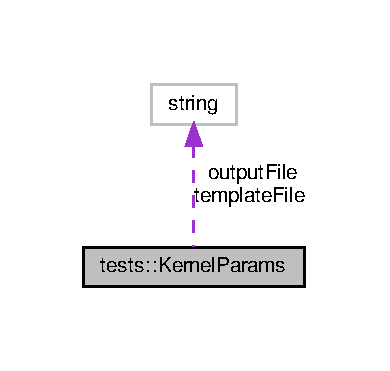
\includegraphics[width=187pt]{structtests_1_1KernelParams__coll__graph}
\end{center}
\end{figure}
\subsection*{Public Attributes}
\begin{DoxyCompactItemize}
\item 
std\+::map$<$ std\+::string, std\+::string $>$ \hyperlink{structtests_1_1KernelParams_a80bd8fec07cf507128923b01df069162}{param\+\_\+mappings} = \{\}
\item 
std\+::string \hyperlink{structtests_1_1KernelParams_aba4e8ce0e7f164dae2e76e492d2dc560}{template\+File} = \char`\"{}\char`\"{}
\item 
std\+::string \hyperlink{structtests_1_1KernelParams_a36fa86475bbc1dd064d1e362f74c0a50}{output\+File} = \char`\"{}\char`\"{}
\end{DoxyCompactItemize}


\subsection{Member Data Documentation}
\mbox{\Hypertarget{structtests_1_1KernelParams_a36fa86475bbc1dd064d1e362f74c0a50}\label{structtests_1_1KernelParams_a36fa86475bbc1dd064d1e362f74c0a50}} 
\index{tests\+::\+Kernel\+Params@{tests\+::\+Kernel\+Params}!output\+File@{output\+File}}
\index{output\+File@{output\+File}!tests\+::\+Kernel\+Params@{tests\+::\+Kernel\+Params}}
\subsubsection{\texorpdfstring{output\+File}{outputFile}}
{\footnotesize\ttfamily std\+::string tests\+::\+Kernel\+Params\+::output\+File = \char`\"{}\char`\"{}}

\mbox{\Hypertarget{structtests_1_1KernelParams_a80bd8fec07cf507128923b01df069162}\label{structtests_1_1KernelParams_a80bd8fec07cf507128923b01df069162}} 
\index{tests\+::\+Kernel\+Params@{tests\+::\+Kernel\+Params}!param\+\_\+mappings@{param\+\_\+mappings}}
\index{param\+\_\+mappings@{param\+\_\+mappings}!tests\+::\+Kernel\+Params@{tests\+::\+Kernel\+Params}}
\subsubsection{\texorpdfstring{param\+\_\+mappings}{param\_mappings}}
{\footnotesize\ttfamily std\+::map$<$std\+::string, std\+::string$>$ tests\+::\+Kernel\+Params\+::param\+\_\+mappings = \{\}}

\mbox{\Hypertarget{structtests_1_1KernelParams_aba4e8ce0e7f164dae2e76e492d2dc560}\label{structtests_1_1KernelParams_aba4e8ce0e7f164dae2e76e492d2dc560}} 
\index{tests\+::\+Kernel\+Params@{tests\+::\+Kernel\+Params}!template\+File@{template\+File}}
\index{template\+File@{template\+File}!tests\+::\+Kernel\+Params@{tests\+::\+Kernel\+Params}}
\subsubsection{\texorpdfstring{template\+File}{templateFile}}
{\footnotesize\ttfamily std\+::string tests\+::\+Kernel\+Params\+::template\+File = \char`\"{}\char`\"{}}



The documentation for this struct was generated from the following file\+:\begin{DoxyCompactItemize}
\item 
tests/\hyperlink{test__kernel__params_8h}{test\+\_\+kernel\+\_\+params.\+h}\end{DoxyCompactItemize}

\hypertarget{classllk_1_1memory}{}\section{llk\+:\+:memory Class Reference}
\label{classllk_1_1memory}\index{llk\+::memory@{llk\+::memory}}


{\ttfamily \#include $<$llk\+\_\+memory.\+h$>$}

\subsection*{Public Types}
\begin{DoxyCompactItemize}
\item 
typedef std\+::uint32\+\_\+t \hyperlink{classllk_1_1memory_ae7a4b897aa999f22e250dc8e4d773dec}{address\+\_\+t}
\item 
typedef std\+::uint32\+\_\+t \hyperlink{classllk_1_1memory_a432a6c0ae1bcb9c44d79cfa1a239419c}{word\+\_\+t}
\end{DoxyCompactItemize}
\subsection*{Public Member Functions}
\begin{DoxyCompactItemize}
\item 
\hyperlink{classllk_1_1memory_a7069a8b6f6ef11b17f2346db9d943204}{memory} ()
\item 
\hyperlink{classllk_1_1memory_a3b2eedc557f34c00cb0a7bc677e1cb5a}{memory} (\hyperlink{classllk_1_1memory_ae7a4b897aa999f22e250dc8e4d773dec}{address\+\_\+t} \hyperlink{classllk_1_1memory_aa31d9d8c64a1b4f7d8dbeec82af0add2}{base}, \hyperlink{classllk_1_1memory_ae7a4b897aa999f22e250dc8e4d773dec}{address\+\_\+t} \hyperlink{classllk_1_1memory_aee316fd12fa52ea8b9884a03f67a8768}{size})
\item 
\hyperlink{classllk_1_1memory_ace253b499ac7e10d49b7e58ded343884}{memory} (\hyperlink{classllk_1_1memory_ae7a4b897aa999f22e250dc8e4d773dec}{address\+\_\+t} \hyperlink{classllk_1_1memory_aa31d9d8c64a1b4f7d8dbeec82af0add2}{base}, const std\+::vector$<$ \hyperlink{classllk_1_1memory_a432a6c0ae1bcb9c44d79cfa1a239419c}{word\+\_\+t} $>$ \&content)
\item 
\hyperlink{classllk_1_1memory_aafdc3d1f68de49e73d640b44fe9e1628}{memory} (\hyperlink{classllk_1_1memory_ae7a4b897aa999f22e250dc8e4d773dec}{address\+\_\+t} \hyperlink{classllk_1_1memory_aa31d9d8c64a1b4f7d8dbeec82af0add2}{base}, std\+::vector$<$ \hyperlink{classllk_1_1memory_a432a6c0ae1bcb9c44d79cfa1a239419c}{word\+\_\+t} $>$ \&\&content)
\item 
void \hyperlink{classllk_1_1memory_aaaa33a11f4fcd7d45f4689ef8e5ccb04}{resize} (std\+::size\+\_\+t num\+\_\+words)
\item 
void \hyperlink{classllk_1_1memory_a584700cdc818d0dad9e44a122f14997b}{load\+\_\+relative\+\_\+hex} (const std\+::string \&filename)
\item 
\hyperlink{classllk_1_1memory_ae7a4b897aa999f22e250dc8e4d773dec}{address\+\_\+t} \hyperlink{classllk_1_1memory_aa31d9d8c64a1b4f7d8dbeec82af0add2}{base} () const
\item 
\hyperlink{classllk_1_1memory_ae7a4b897aa999f22e250dc8e4d773dec}{address\+\_\+t} \hyperlink{classllk_1_1memory_aee316fd12fa52ea8b9884a03f67a8768}{size} () const
\item 
\hyperlink{classllk_1_1memory_ae7a4b897aa999f22e250dc8e4d773dec}{address\+\_\+t} \hyperlink{classllk_1_1memory_a81eb269512a86baf7e9cd560e44e0d41}{limit} () const
\item 
\hyperlink{classllk_1_1memory_ae7a4b897aa999f22e250dc8e4d773dec}{address\+\_\+t} \hyperlink{classllk_1_1memory_aa87483dcd1f592e288a4191e435d2ad3}{base\+\_\+word} () const
\item 
\hyperlink{classllk_1_1memory_ae7a4b897aa999f22e250dc8e4d773dec}{address\+\_\+t} \hyperlink{classllk_1_1memory_a5efebebcf80bc1d7f9314ac0e046ee41}{count} () const
\item 
\hyperlink{classllk_1_1memory_ae7a4b897aa999f22e250dc8e4d773dec}{address\+\_\+t} \hyperlink{classllk_1_1memory_a8ed2fac7f82609c47e58bf4774b05b74}{limit\+\_\+word} () const
\item 
decltype(auto) \hyperlink{classllk_1_1memory_a8227a4de6153b8814568474726d02f24}{operator\mbox{[}$\,$\mbox{]}} (\hyperlink{classllk_1_1memory_ae7a4b897aa999f22e250dc8e4d773dec}{address\+\_\+t} i) const
\item 
decltype(auto) \hyperlink{classllk_1_1memory_aefa4c0ffc2836b50f88d3f67c68eb9b6}{operator\mbox{[}$\,$\mbox{]}} (\hyperlink{classllk_1_1memory_ae7a4b897aa999f22e250dc8e4d773dec}{address\+\_\+t} i)
\item 
\hyperlink{classllk_1_1memory_a432a6c0ae1bcb9c44d79cfa1a239419c}{word\+\_\+t} $\ast$ \hyperlink{classllk_1_1memory_a5d840d8417c2cdb37ec1f77ecb0fec6e}{data} ()
\item 
const \hyperlink{classllk_1_1memory_a432a6c0ae1bcb9c44d79cfa1a239419c}{word\+\_\+t} $\ast$ \hyperlink{classllk_1_1memory_aea2feb3e69edfa3968fcc715d7a05238}{data} () const
\item 
void \hyperlink{classllk_1_1memory_a1a8f5221024e8bec67843782a5e511a0}{write\+\_\+hex} (std\+::ostream \&os) const
\item 
auto \hyperlink{classllk_1_1memory_aebeb9c5ccea123bc09ecd2667756af91}{consume} () \&\&
\item 
auto \hyperlink{classllk_1_1memory_abdb3f8fa8d0c1b700dfb02d616b02bd2}{contents} ()
\item 
bool \hyperlink{classllk_1_1memory_a268d76a85a246184d5f1d9bb00b57712}{operator==} (const \hyperlink{classllk_1_1memory}{memory} \&rhs) const
\item 
std\+::string \hyperlink{classllk_1_1memory_aa6e946fd02850a01a1a30f56c28ef530}{to\+\_\+string} ()
\item 
\hyperlink{classllk_1_1memory_a68a9ba98730a540ab25d5c21e9501790}{operator Command\+Assembler\+::memory} () const
\end{DoxyCompactItemize}
\subsection*{Static Public Member Functions}
\begin{DoxyCompactItemize}
\item 
static \hyperlink{classllk_1_1memory}{memory} \hyperlink{classllk_1_1memory_a21247daa4aa05ac0e4841c7771e68feb}{from\+\_\+contiguous\+\_\+hex} (std\+::istream \&is)
\begin{DoxyCompactList}\small\item\em Read from {\ttfamily is} to create a memory that is exactly the size of the hex. \end{DoxyCompactList}\item 
static \hyperlink{classllk_1_1memory}{memory} \hyperlink{classllk_1_1memory_a442c8533296f44afb2152129417e02ba}{load\+\_\+hex} (std\+::istream \&is)
\item 
static \hyperlink{classllk_1_1memory}{memory} \hyperlink{classllk_1_1memory_a86fbd7265d551f2e18e943028d2b8728}{from\+\_\+discontiguous\+\_\+hex} (std\+::istream \&is)
\begin{DoxyCompactList}\small\item\em Read from {\ttfamily is} to create a memory that encompasses all assigned addresses. Other locations will be 0. \end{DoxyCompactList}\end{DoxyCompactItemize}
\subsection*{Friends}
\begin{DoxyCompactItemize}
\item 
std\+::ostream \& \hyperlink{classllk_1_1memory_aed852dd183dc752b9fc575dbe2113c1d}{operator$<$$<$} (std\+::ostream \&os, const \hyperlink{classllk_1_1memory}{memory} \&mem)
\end{DoxyCompactItemize}


\subsection{Member Typedef Documentation}
\mbox{\Hypertarget{classllk_1_1memory_ae7a4b897aa999f22e250dc8e4d773dec}\label{classllk_1_1memory_ae7a4b897aa999f22e250dc8e4d773dec}} 
\index{llk\+::memory@{llk\+::memory}!address\+\_\+t@{address\+\_\+t}}
\index{address\+\_\+t@{address\+\_\+t}!llk\+::memory@{llk\+::memory}}
\subsubsection{\texorpdfstring{address\+\_\+t}{address\_t}}
{\footnotesize\ttfamily typedef std\+::uint32\+\_\+t \hyperlink{classllk_1_1memory_ae7a4b897aa999f22e250dc8e4d773dec}{llk\+::memory\+::address\+\_\+t}}

\mbox{\Hypertarget{classllk_1_1memory_a432a6c0ae1bcb9c44d79cfa1a239419c}\label{classllk_1_1memory_a432a6c0ae1bcb9c44d79cfa1a239419c}} 
\index{llk\+::memory@{llk\+::memory}!word\+\_\+t@{word\+\_\+t}}
\index{word\+\_\+t@{word\+\_\+t}!llk\+::memory@{llk\+::memory}}
\subsubsection{\texorpdfstring{word\+\_\+t}{word\_t}}
{\footnotesize\ttfamily typedef std\+::uint32\+\_\+t \hyperlink{classllk_1_1memory_a432a6c0ae1bcb9c44d79cfa1a239419c}{llk\+::memory\+::word\+\_\+t}}



\subsection{Constructor \& Destructor Documentation}
\mbox{\Hypertarget{classllk_1_1memory_a7069a8b6f6ef11b17f2346db9d943204}\label{classllk_1_1memory_a7069a8b6f6ef11b17f2346db9d943204}} 
\index{llk\+::memory@{llk\+::memory}!memory@{memory}}
\index{memory@{memory}!llk\+::memory@{llk\+::memory}}
\subsubsection{\texorpdfstring{memory()}{memory()}\hspace{0.1cm}{\footnotesize\ttfamily [1/4]}}
{\footnotesize\ttfamily llk\+::memory\+::memory (\begin{DoxyParamCaption}{ }\end{DoxyParamCaption})\hspace{0.3cm}{\ttfamily [inline]}}

\mbox{\Hypertarget{classllk_1_1memory_a3b2eedc557f34c00cb0a7bc677e1cb5a}\label{classllk_1_1memory_a3b2eedc557f34c00cb0a7bc677e1cb5a}} 
\index{llk\+::memory@{llk\+::memory}!memory@{memory}}
\index{memory@{memory}!llk\+::memory@{llk\+::memory}}
\subsubsection{\texorpdfstring{memory()}{memory()}\hspace{0.1cm}{\footnotesize\ttfamily [2/4]}}
{\footnotesize\ttfamily llk\+::memory\+::memory (\begin{DoxyParamCaption}\item[{\hyperlink{classllk_1_1memory_ae7a4b897aa999f22e250dc8e4d773dec}{address\+\_\+t}}]{base,  }\item[{\hyperlink{classllk_1_1memory_ae7a4b897aa999f22e250dc8e4d773dec}{address\+\_\+t}}]{size }\end{DoxyParamCaption})}

\mbox{\Hypertarget{classllk_1_1memory_ace253b499ac7e10d49b7e58ded343884}\label{classllk_1_1memory_ace253b499ac7e10d49b7e58ded343884}} 
\index{llk\+::memory@{llk\+::memory}!memory@{memory}}
\index{memory@{memory}!llk\+::memory@{llk\+::memory}}
\subsubsection{\texorpdfstring{memory()}{memory()}\hspace{0.1cm}{\footnotesize\ttfamily [3/4]}}
{\footnotesize\ttfamily llk\+::memory\+::memory (\begin{DoxyParamCaption}\item[{\hyperlink{classllk_1_1memory_ae7a4b897aa999f22e250dc8e4d773dec}{address\+\_\+t}}]{base,  }\item[{const std\+::vector$<$ \hyperlink{classllk_1_1memory_a432a6c0ae1bcb9c44d79cfa1a239419c}{word\+\_\+t} $>$ \&}]{content }\end{DoxyParamCaption})}

\mbox{\Hypertarget{classllk_1_1memory_aafdc3d1f68de49e73d640b44fe9e1628}\label{classllk_1_1memory_aafdc3d1f68de49e73d640b44fe9e1628}} 
\index{llk\+::memory@{llk\+::memory}!memory@{memory}}
\index{memory@{memory}!llk\+::memory@{llk\+::memory}}
\subsubsection{\texorpdfstring{memory()}{memory()}\hspace{0.1cm}{\footnotesize\ttfamily [4/4]}}
{\footnotesize\ttfamily llk\+::memory\+::memory (\begin{DoxyParamCaption}\item[{\hyperlink{classllk_1_1memory_ae7a4b897aa999f22e250dc8e4d773dec}{address\+\_\+t}}]{base,  }\item[{std\+::vector$<$ \hyperlink{classllk_1_1memory_a432a6c0ae1bcb9c44d79cfa1a239419c}{word\+\_\+t} $>$ \&\&}]{content }\end{DoxyParamCaption})}



\subsection{Member Function Documentation}
\mbox{\Hypertarget{classllk_1_1memory_aa31d9d8c64a1b4f7d8dbeec82af0add2}\label{classllk_1_1memory_aa31d9d8c64a1b4f7d8dbeec82af0add2}} 
\index{llk\+::memory@{llk\+::memory}!base@{base}}
\index{base@{base}!llk\+::memory@{llk\+::memory}}
\subsubsection{\texorpdfstring{base()}{base()}}
{\footnotesize\ttfamily \hyperlink{classllk_1_1memory_ae7a4b897aa999f22e250dc8e4d773dec}{address\+\_\+t} llk\+::memory\+::base (\begin{DoxyParamCaption}{ }\end{DoxyParamCaption}) const\hspace{0.3cm}{\ttfamily [inline]}}

\mbox{\Hypertarget{classllk_1_1memory_aa87483dcd1f592e288a4191e435d2ad3}\label{classllk_1_1memory_aa87483dcd1f592e288a4191e435d2ad3}} 
\index{llk\+::memory@{llk\+::memory}!base\+\_\+word@{base\+\_\+word}}
\index{base\+\_\+word@{base\+\_\+word}!llk\+::memory@{llk\+::memory}}
\subsubsection{\texorpdfstring{base\+\_\+word()}{base\_word()}}
{\footnotesize\ttfamily \hyperlink{classllk_1_1memory_ae7a4b897aa999f22e250dc8e4d773dec}{address\+\_\+t} llk\+::memory\+::base\+\_\+word (\begin{DoxyParamCaption}{ }\end{DoxyParamCaption}) const\hspace{0.3cm}{\ttfamily [inline]}}

\mbox{\Hypertarget{classllk_1_1memory_aebeb9c5ccea123bc09ecd2667756af91}\label{classllk_1_1memory_aebeb9c5ccea123bc09ecd2667756af91}} 
\index{llk\+::memory@{llk\+::memory}!consume@{consume}}
\index{consume@{consume}!llk\+::memory@{llk\+::memory}}
\subsubsection{\texorpdfstring{consume()}{consume()}}
{\footnotesize\ttfamily auto llk\+::memory\+::consume (\begin{DoxyParamCaption}{ }\end{DoxyParamCaption}) \&\&\hspace{0.3cm}{\ttfamily [inline]}}

\mbox{\Hypertarget{classllk_1_1memory_abdb3f8fa8d0c1b700dfb02d616b02bd2}\label{classllk_1_1memory_abdb3f8fa8d0c1b700dfb02d616b02bd2}} 
\index{llk\+::memory@{llk\+::memory}!contents@{contents}}
\index{contents@{contents}!llk\+::memory@{llk\+::memory}}
\subsubsection{\texorpdfstring{contents()}{contents()}}
{\footnotesize\ttfamily auto llk\+::memory\+::contents (\begin{DoxyParamCaption}{ }\end{DoxyParamCaption})\hspace{0.3cm}{\ttfamily [inline]}}

\mbox{\Hypertarget{classllk_1_1memory_a5efebebcf80bc1d7f9314ac0e046ee41}\label{classllk_1_1memory_a5efebebcf80bc1d7f9314ac0e046ee41}} 
\index{llk\+::memory@{llk\+::memory}!count@{count}}
\index{count@{count}!llk\+::memory@{llk\+::memory}}
\subsubsection{\texorpdfstring{count()}{count()}}
{\footnotesize\ttfamily \hyperlink{classllk_1_1memory_ae7a4b897aa999f22e250dc8e4d773dec}{address\+\_\+t} llk\+::memory\+::count (\begin{DoxyParamCaption}{ }\end{DoxyParamCaption}) const\hspace{0.3cm}{\ttfamily [inline]}}

\mbox{\Hypertarget{classllk_1_1memory_a5d840d8417c2cdb37ec1f77ecb0fec6e}\label{classllk_1_1memory_a5d840d8417c2cdb37ec1f77ecb0fec6e}} 
\index{llk\+::memory@{llk\+::memory}!data@{data}}
\index{data@{data}!llk\+::memory@{llk\+::memory}}
\subsubsection{\texorpdfstring{data()}{data()}\hspace{0.1cm}{\footnotesize\ttfamily [1/2]}}
{\footnotesize\ttfamily \hyperlink{classllk_1_1memory_a432a6c0ae1bcb9c44d79cfa1a239419c}{word\+\_\+t}$\ast$ llk\+::memory\+::data (\begin{DoxyParamCaption}{ }\end{DoxyParamCaption})\hspace{0.3cm}{\ttfamily [inline]}}

\mbox{\Hypertarget{classllk_1_1memory_aea2feb3e69edfa3968fcc715d7a05238}\label{classllk_1_1memory_aea2feb3e69edfa3968fcc715d7a05238}} 
\index{llk\+::memory@{llk\+::memory}!data@{data}}
\index{data@{data}!llk\+::memory@{llk\+::memory}}
\subsubsection{\texorpdfstring{data()}{data()}\hspace{0.1cm}{\footnotesize\ttfamily [2/2]}}
{\footnotesize\ttfamily const \hyperlink{classllk_1_1memory_a432a6c0ae1bcb9c44d79cfa1a239419c}{word\+\_\+t}$\ast$ llk\+::memory\+::data (\begin{DoxyParamCaption}{ }\end{DoxyParamCaption}) const\hspace{0.3cm}{\ttfamily [inline]}}

\mbox{\Hypertarget{classllk_1_1memory_a21247daa4aa05ac0e4841c7771e68feb}\label{classllk_1_1memory_a21247daa4aa05ac0e4841c7771e68feb}} 
\index{llk\+::memory@{llk\+::memory}!from\+\_\+contiguous\+\_\+hex@{from\+\_\+contiguous\+\_\+hex}}
\index{from\+\_\+contiguous\+\_\+hex@{from\+\_\+contiguous\+\_\+hex}!llk\+::memory@{llk\+::memory}}
\subsubsection{\texorpdfstring{from\+\_\+contiguous\+\_\+hex()}{from\_contiguous\_hex()}}
{\footnotesize\ttfamily \hyperlink{classllk_1_1memory}{memory} llk\+::memory\+::from\+\_\+contiguous\+\_\+hex (\begin{DoxyParamCaption}\item[{std\+::istream \&}]{is }\end{DoxyParamCaption})\hspace{0.3cm}{\ttfamily [static]}}



Read from {\ttfamily is} to create a memory that is exactly the size of the hex. 

Multiple @ lines will cause an exception to be thrown. \mbox{\Hypertarget{classllk_1_1memory_a86fbd7265d551f2e18e943028d2b8728}\label{classllk_1_1memory_a86fbd7265d551f2e18e943028d2b8728}} 
\index{llk\+::memory@{llk\+::memory}!from\+\_\+discontiguous\+\_\+hex@{from\+\_\+discontiguous\+\_\+hex}}
\index{from\+\_\+discontiguous\+\_\+hex@{from\+\_\+discontiguous\+\_\+hex}!llk\+::memory@{llk\+::memory}}
\subsubsection{\texorpdfstring{from\+\_\+discontiguous\+\_\+hex()}{from\_discontiguous\_hex()}}
{\footnotesize\ttfamily \hyperlink{classllk_1_1memory}{memory} llk\+::memory\+::from\+\_\+discontiguous\+\_\+hex (\begin{DoxyParamCaption}\item[{std\+::istream \&}]{is }\end{DoxyParamCaption})\hspace{0.3cm}{\ttfamily [static]}}



Read from {\ttfamily is} to create a memory that encompasses all assigned addresses. Other locations will be 0. 

Can have as many @ lines as necessary. \mbox{\Hypertarget{classllk_1_1memory_a81eb269512a86baf7e9cd560e44e0d41}\label{classllk_1_1memory_a81eb269512a86baf7e9cd560e44e0d41}} 
\index{llk\+::memory@{llk\+::memory}!limit@{limit}}
\index{limit@{limit}!llk\+::memory@{llk\+::memory}}
\subsubsection{\texorpdfstring{limit()}{limit()}}
{\footnotesize\ttfamily \hyperlink{classllk_1_1memory_ae7a4b897aa999f22e250dc8e4d773dec}{address\+\_\+t} llk\+::memory\+::limit (\begin{DoxyParamCaption}{ }\end{DoxyParamCaption}) const\hspace{0.3cm}{\ttfamily [inline]}}

\mbox{\Hypertarget{classllk_1_1memory_a8ed2fac7f82609c47e58bf4774b05b74}\label{classllk_1_1memory_a8ed2fac7f82609c47e58bf4774b05b74}} 
\index{llk\+::memory@{llk\+::memory}!limit\+\_\+word@{limit\+\_\+word}}
\index{limit\+\_\+word@{limit\+\_\+word}!llk\+::memory@{llk\+::memory}}
\subsubsection{\texorpdfstring{limit\+\_\+word()}{limit\_word()}}
{\footnotesize\ttfamily \hyperlink{classllk_1_1memory_ae7a4b897aa999f22e250dc8e4d773dec}{address\+\_\+t} llk\+::memory\+::limit\+\_\+word (\begin{DoxyParamCaption}{ }\end{DoxyParamCaption}) const\hspace{0.3cm}{\ttfamily [inline]}}

\mbox{\Hypertarget{classllk_1_1memory_a442c8533296f44afb2152129417e02ba}\label{classllk_1_1memory_a442c8533296f44afb2152129417e02ba}} 
\index{llk\+::memory@{llk\+::memory}!load\+\_\+hex@{load\+\_\+hex}}
\index{load\+\_\+hex@{load\+\_\+hex}!llk\+::memory@{llk\+::memory}}
\subsubsection{\texorpdfstring{load\+\_\+hex()}{load\_hex()}}
{\footnotesize\ttfamily static \hyperlink{classllk_1_1memory}{memory} llk\+::memory\+::load\+\_\+hex (\begin{DoxyParamCaption}\item[{std\+::istream \&}]{is }\end{DoxyParamCaption})\hspace{0.3cm}{\ttfamily [inline]}, {\ttfamily [static]}}

\mbox{\Hypertarget{classllk_1_1memory_a584700cdc818d0dad9e44a122f14997b}\label{classllk_1_1memory_a584700cdc818d0dad9e44a122f14997b}} 
\index{llk\+::memory@{llk\+::memory}!load\+\_\+relative\+\_\+hex@{load\+\_\+relative\+\_\+hex}}
\index{load\+\_\+relative\+\_\+hex@{load\+\_\+relative\+\_\+hex}!llk\+::memory@{llk\+::memory}}
\subsubsection{\texorpdfstring{load\+\_\+relative\+\_\+hex()}{load\_relative\_hex()}}
{\footnotesize\ttfamily void llk\+::memory\+::load\+\_\+relative\+\_\+hex (\begin{DoxyParamCaption}\item[{const std\+::string \&}]{filename }\end{DoxyParamCaption})}

\mbox{\Hypertarget{classllk_1_1memory_a68a9ba98730a540ab25d5c21e9501790}\label{classllk_1_1memory_a68a9ba98730a540ab25d5c21e9501790}} 
\index{llk\+::memory@{llk\+::memory}!operator Command\+Assembler\+::memory@{operator Command\+Assembler\+::memory}}
\index{operator Command\+Assembler\+::memory@{operator Command\+Assembler\+::memory}!llk\+::memory@{llk\+::memory}}
\subsubsection{\texorpdfstring{operator Command\+Assembler\+::memory()}{operator CommandAssembler::memory()}}
{\footnotesize\ttfamily llk\+::memory\+::operator Command\+Assembler\+::memory (\begin{DoxyParamCaption}{ }\end{DoxyParamCaption}) const\hspace{0.3cm}{\ttfamily [inline]}}

\mbox{\Hypertarget{classllk_1_1memory_a268d76a85a246184d5f1d9bb00b57712}\label{classllk_1_1memory_a268d76a85a246184d5f1d9bb00b57712}} 
\index{llk\+::memory@{llk\+::memory}!operator==@{operator==}}
\index{operator==@{operator==}!llk\+::memory@{llk\+::memory}}
\subsubsection{\texorpdfstring{operator==()}{operator==()}}
{\footnotesize\ttfamily bool llk\+::memory\+::operator== (\begin{DoxyParamCaption}\item[{const \hyperlink{classllk_1_1memory}{memory} \&}]{rhs }\end{DoxyParamCaption}) const\hspace{0.3cm}{\ttfamily [inline]}}

\mbox{\Hypertarget{classllk_1_1memory_a8227a4de6153b8814568474726d02f24}\label{classllk_1_1memory_a8227a4de6153b8814568474726d02f24}} 
\index{llk\+::memory@{llk\+::memory}!operator\mbox{[}\mbox{]}@{operator[]}}
\index{operator\mbox{[}\mbox{]}@{operator[]}!llk\+::memory@{llk\+::memory}}
\subsubsection{\texorpdfstring{operator[]()}{operator[]()}\hspace{0.1cm}{\footnotesize\ttfamily [1/2]}}
{\footnotesize\ttfamily decltype(auto) llk\+::memory\+::operator\mbox{[}$\,$\mbox{]} (\begin{DoxyParamCaption}\item[{\hyperlink{classllk_1_1memory_ae7a4b897aa999f22e250dc8e4d773dec}{address\+\_\+t}}]{i }\end{DoxyParamCaption}) const\hspace{0.3cm}{\ttfamily [inline]}}

\mbox{\Hypertarget{classllk_1_1memory_aefa4c0ffc2836b50f88d3f67c68eb9b6}\label{classllk_1_1memory_aefa4c0ffc2836b50f88d3f67c68eb9b6}} 
\index{llk\+::memory@{llk\+::memory}!operator\mbox{[}\mbox{]}@{operator[]}}
\index{operator\mbox{[}\mbox{]}@{operator[]}!llk\+::memory@{llk\+::memory}}
\subsubsection{\texorpdfstring{operator[]()}{operator[]()}\hspace{0.1cm}{\footnotesize\ttfamily [2/2]}}
{\footnotesize\ttfamily decltype(auto) llk\+::memory\+::operator\mbox{[}$\,$\mbox{]} (\begin{DoxyParamCaption}\item[{\hyperlink{classllk_1_1memory_ae7a4b897aa999f22e250dc8e4d773dec}{address\+\_\+t}}]{i }\end{DoxyParamCaption})\hspace{0.3cm}{\ttfamily [inline]}}

\mbox{\Hypertarget{classllk_1_1memory_aaaa33a11f4fcd7d45f4689ef8e5ccb04}\label{classllk_1_1memory_aaaa33a11f4fcd7d45f4689ef8e5ccb04}} 
\index{llk\+::memory@{llk\+::memory}!resize@{resize}}
\index{resize@{resize}!llk\+::memory@{llk\+::memory}}
\subsubsection{\texorpdfstring{resize()}{resize()}}
{\footnotesize\ttfamily void llk\+::memory\+::resize (\begin{DoxyParamCaption}\item[{std\+::size\+\_\+t}]{num\+\_\+words }\end{DoxyParamCaption})\hspace{0.3cm}{\ttfamily [inline]}}

\mbox{\Hypertarget{classllk_1_1memory_aee316fd12fa52ea8b9884a03f67a8768}\label{classllk_1_1memory_aee316fd12fa52ea8b9884a03f67a8768}} 
\index{llk\+::memory@{llk\+::memory}!size@{size}}
\index{size@{size}!llk\+::memory@{llk\+::memory}}
\subsubsection{\texorpdfstring{size()}{size()}}
{\footnotesize\ttfamily \hyperlink{classllk_1_1memory_ae7a4b897aa999f22e250dc8e4d773dec}{address\+\_\+t} llk\+::memory\+::size (\begin{DoxyParamCaption}{ }\end{DoxyParamCaption}) const\hspace{0.3cm}{\ttfamily [inline]}}

\mbox{\Hypertarget{classllk_1_1memory_aa6e946fd02850a01a1a30f56c28ef530}\label{classllk_1_1memory_aa6e946fd02850a01a1a30f56c28ef530}} 
\index{llk\+::memory@{llk\+::memory}!to\+\_\+string@{to\+\_\+string}}
\index{to\+\_\+string@{to\+\_\+string}!llk\+::memory@{llk\+::memory}}
\subsubsection{\texorpdfstring{to\+\_\+string()}{to\_string()}}
{\footnotesize\ttfamily std\+::string llk\+::memory\+::to\+\_\+string (\begin{DoxyParamCaption}{ }\end{DoxyParamCaption})\hspace{0.3cm}{\ttfamily [inline]}}

\mbox{\Hypertarget{classllk_1_1memory_a1a8f5221024e8bec67843782a5e511a0}\label{classllk_1_1memory_a1a8f5221024e8bec67843782a5e511a0}} 
\index{llk\+::memory@{llk\+::memory}!write\+\_\+hex@{write\+\_\+hex}}
\index{write\+\_\+hex@{write\+\_\+hex}!llk\+::memory@{llk\+::memory}}
\subsubsection{\texorpdfstring{write\+\_\+hex()}{write\_hex()}}
{\footnotesize\ttfamily void llk\+::memory\+::write\+\_\+hex (\begin{DoxyParamCaption}\item[{std\+::ostream \&}]{os }\end{DoxyParamCaption}) const}



\subsection{Friends And Related Function Documentation}
\mbox{\Hypertarget{classllk_1_1memory_aed852dd183dc752b9fc575dbe2113c1d}\label{classllk_1_1memory_aed852dd183dc752b9fc575dbe2113c1d}} 
\index{llk\+::memory@{llk\+::memory}!operator$<$$<$@{operator$<$$<$}}
\index{operator$<$$<$@{operator$<$$<$}!llk\+::memory@{llk\+::memory}}
\subsubsection{\texorpdfstring{operator$<$$<$}{operator<<}}
{\footnotesize\ttfamily std\+::ostream\& operator$<$$<$ (\begin{DoxyParamCaption}\item[{std\+::ostream \&}]{os,  }\item[{const \hyperlink{classllk_1_1memory}{memory} \&}]{mem }\end{DoxyParamCaption})\hspace{0.3cm}{\ttfamily [friend]}}



The documentation for this class was generated from the following files\+:\begin{DoxyCompactItemize}
\item 
inc/\hyperlink{llk__memory_8h}{llk\+\_\+memory.\+h}\item 
src/\hyperlink{llk__memory_8cpp}{llk\+\_\+memory.\+cpp}\end{DoxyCompactItemize}

\hypertarget{structtests_1_1OverlayConfig}{}\section{tests\+:\+:Overlay\+Config Struct Reference}
\label{structtests_1_1OverlayConfig}\index{tests\+::\+Overlay\+Config@{tests\+::\+Overlay\+Config}}


{\ttfamily \#include $<$test\+\_\+overlay\+\_\+config.\+h$>$}



Collaboration diagram for tests\+:\+:Overlay\+Config\+:\nopagebreak
\begin{figure}[H]
\begin{center}
\leavevmode
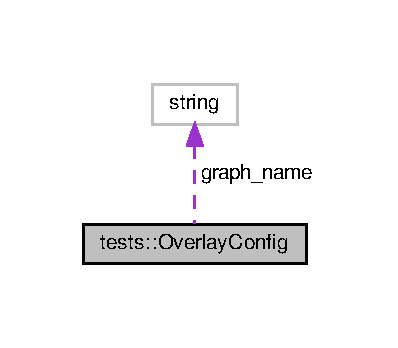
\includegraphics[width=191pt]{structtests_1_1OverlayConfig__coll__graph}
\end{center}
\end{figure}
\subsection*{Public Attributes}
\begin{DoxyCompactItemize}
\item 
std\+::string \hyperlink{structtests_1_1OverlayConfig_a689d5f8a0c184b90d2efc491014c8d1e}{graph\+\_\+name}
\item 
std\+::map$<$ std\+::string, std\+::string $>$ \hyperlink{structtests_1_1OverlayConfig_a52f95fa0ae5619699aaca1ff497a1a0a}{config}
\end{DoxyCompactItemize}


\subsection{Member Data Documentation}
\mbox{\Hypertarget{structtests_1_1OverlayConfig_a52f95fa0ae5619699aaca1ff497a1a0a}\label{structtests_1_1OverlayConfig_a52f95fa0ae5619699aaca1ff497a1a0a}} 
\index{tests\+::\+Overlay\+Config@{tests\+::\+Overlay\+Config}!config@{config}}
\index{config@{config}!tests\+::\+Overlay\+Config@{tests\+::\+Overlay\+Config}}
\subsubsection{\texorpdfstring{config}{config}}
{\footnotesize\ttfamily std\+::map$<$std\+::string, std\+::string$>$ tests\+::\+Overlay\+Config\+::config}

\mbox{\Hypertarget{structtests_1_1OverlayConfig_a689d5f8a0c184b90d2efc491014c8d1e}\label{structtests_1_1OverlayConfig_a689d5f8a0c184b90d2efc491014c8d1e}} 
\index{tests\+::\+Overlay\+Config@{tests\+::\+Overlay\+Config}!graph\+\_\+name@{graph\+\_\+name}}
\index{graph\+\_\+name@{graph\+\_\+name}!tests\+::\+Overlay\+Config@{tests\+::\+Overlay\+Config}}
\subsubsection{\texorpdfstring{graph\+\_\+name}{graph\_name}}
{\footnotesize\ttfamily std\+::string tests\+::\+Overlay\+Config\+::graph\+\_\+name}



The documentation for this struct was generated from the following file\+:\begin{DoxyCompactItemize}
\item 
tests/\hyperlink{test__overlay__config_8h}{test\+\_\+overlay\+\_\+config.\+h}\end{DoxyCompactItemize}

\hypertarget{structtests_1_1SingleCoreTestConfig}{}\section{tests\+:\+:Single\+Core\+Test\+Config Struct Reference}
\label{structtests_1_1SingleCoreTestConfig}\index{tests\+::\+Single\+Core\+Test\+Config@{tests\+::\+Single\+Core\+Test\+Config}}


\hyperlink{structtests_1_1TestConfig}{Test\+Config} specification for a specific core.  




{\ttfamily \#include $<$test\+\_\+config.\+h$>$}

\subsection*{Public Attributes}
\begin{DoxyCompactItemize}
\item 
map$<$ \hyperlink{namespacetests_a4f360b8af533762256ff97513bfd6a0d}{Kernel\+Type}, map$<$ string, string $>$ $>$ \hyperlink{structtests_1_1SingleCoreTestConfig_a58d9652e2888f2a8fd20d1df5419f91e}{kernel\+\_\+names}
\begin{DoxyCompactList}\small\item\em Kernel name has two fields for each kernel type, \char`\"{}base\char`\"{} for param file name generation and \char`\"{}full\char`\"{} which is the full name of kernel. \end{DoxyCompactList}\item 
map$<$ \hyperlink{namespacetests_a4f360b8af533762256ff97513bfd6a0d}{Kernel\+Type}, \hyperlink{structtests_1_1KernelParams}{Kernel\+Params} $>$ \hyperlink{structtests_1_1SingleCoreTestConfig_a7d92aead3b33ee501ebce274d164e8df}{kernel\+\_\+parameters}
\begin{DoxyCompactList}\small\item\em Kernel params has a map$<$string, string$>$ for each kernel type. \end{DoxyCompactList}\end{DoxyCompactItemize}


\subsection{Detailed Description}
\hyperlink{structtests_1_1TestConfig}{Test\+Config} specification for a specific core. 

\subsection{Member Data Documentation}
\mbox{\Hypertarget{structtests_1_1SingleCoreTestConfig_a58d9652e2888f2a8fd20d1df5419f91e}\label{structtests_1_1SingleCoreTestConfig_a58d9652e2888f2a8fd20d1df5419f91e}} 
\index{tests\+::\+Single\+Core\+Test\+Config@{tests\+::\+Single\+Core\+Test\+Config}!kernel\+\_\+names@{kernel\+\_\+names}}
\index{kernel\+\_\+names@{kernel\+\_\+names}!tests\+::\+Single\+Core\+Test\+Config@{tests\+::\+Single\+Core\+Test\+Config}}
\subsubsection{\texorpdfstring{kernel\+\_\+names}{kernel\_names}}
{\footnotesize\ttfamily map$<$\hyperlink{namespacetests_a4f360b8af533762256ff97513bfd6a0d}{Kernel\+Type}, map$<$string, string$>$ $>$ tests\+::\+Single\+Core\+Test\+Config\+::kernel\+\_\+names}

{\bfseries Initial value\+:}
\begin{DoxyCode}
= \{
      \{\hyperlink{namespacetests_a4f360b8af533762256ff97513bfd6a0daba3bbf795bfdbe156772d8f44833a3af}{KernelType::UNPACK}, \{\{\textcolor{stringliteral}{"base"}, \textcolor{stringliteral}{""}\}, \{\textcolor{stringliteral}{"full"}, \textcolor{stringliteral}{""}\}\}\},
      \{\hyperlink{namespacetests_a4f360b8af533762256ff97513bfd6a0da7b849aa2899a63a2da359bf9a0b5b0af}{KernelType::MATH}, \{\{\textcolor{stringliteral}{"base"}, \textcolor{stringliteral}{""}\}, \{\textcolor{stringliteral}{"full"}, \textcolor{stringliteral}{""}\}\}\},
      \{\hyperlink{namespacetests_a4f360b8af533762256ff97513bfd6a0daa484d944b59301977fbe221d69d58857}{KernelType::PACK}, \{\{\textcolor{stringliteral}{"base"}, \textcolor{stringliteral}{""}\}, \{\textcolor{stringliteral}{"full"}, \textcolor{stringliteral}{""}\}\}\},
  \}
\end{DoxyCode}


Kernel name has two fields for each kernel type, \char`\"{}base\char`\"{} for param file name generation and \char`\"{}full\char`\"{} which is the full name of kernel. 

\mbox{\Hypertarget{structtests_1_1SingleCoreTestConfig_a7d92aead3b33ee501ebce274d164e8df}\label{structtests_1_1SingleCoreTestConfig_a7d92aead3b33ee501ebce274d164e8df}} 
\index{tests\+::\+Single\+Core\+Test\+Config@{tests\+::\+Single\+Core\+Test\+Config}!kernel\+\_\+parameters@{kernel\+\_\+parameters}}
\index{kernel\+\_\+parameters@{kernel\+\_\+parameters}!tests\+::\+Single\+Core\+Test\+Config@{tests\+::\+Single\+Core\+Test\+Config}}
\subsubsection{\texorpdfstring{kernel\+\_\+parameters}{kernel\_parameters}}
{\footnotesize\ttfamily map$<$\hyperlink{namespacetests_a4f360b8af533762256ff97513bfd6a0d}{Kernel\+Type}, \hyperlink{structtests_1_1KernelParams}{Kernel\+Params}$>$ tests\+::\+Single\+Core\+Test\+Config\+::kernel\+\_\+parameters}

{\bfseries Initial value\+:}
\begin{DoxyCode}
= \{
      \{\hyperlink{namespacetests_a4f360b8af533762256ff97513bfd6a0daba3bbf795bfdbe156772d8f44833a3af}{KernelType::UNPACK}, KernelParams()\},
      \{\hyperlink{namespacetests_a4f360b8af533762256ff97513bfd6a0da7b849aa2899a63a2da359bf9a0b5b0af}{KernelType::MATH}, KernelParams()\},
      \{\hyperlink{namespacetests_a4f360b8af533762256ff97513bfd6a0daa484d944b59301977fbe221d69d58857}{KernelType::PACK}, KernelParams()\},
  \}
\end{DoxyCode}


Kernel params has a map$<$string, string$>$ for each kernel type. 



The documentation for this struct was generated from the following file\+:\begin{DoxyCompactItemize}
\item 
tests/\hyperlink{test__config_8h}{test\+\_\+config.\+h}\end{DoxyCompactItemize}

\hypertarget{structllk_1_1SocDescriptor}{}\section{llk\+:\+:Soc\+Descriptor Struct Reference}
\label{structllk_1_1SocDescriptor}\index{llk\+::\+Soc\+Descriptor@{llk\+::\+Soc\+Descriptor}}


\hyperlink{structllk_1_1SocDescriptor}{Soc\+Descriptor} contains information regarding the S\+OC configuration targetted.  




{\ttfamily \#include $<$llk\+\_\+soc\+\_\+descriptor.\+h$>$}



Collaboration diagram for llk\+:\+:Soc\+Descriptor\+:\nopagebreak
\begin{figure}[H]
\begin{center}
\leavevmode
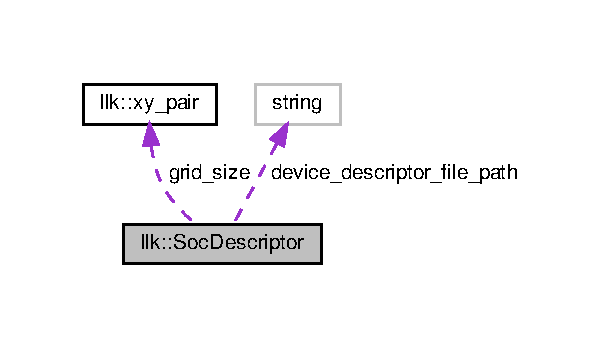
\includegraphics[width=289pt]{structllk_1_1SocDescriptor__coll__graph}
\end{center}
\end{figure}
\subsection*{Public Member Functions}
\begin{DoxyCompactItemize}
\item 
const bool \hyperlink{structllk_1_1SocDescriptor_a5c4fdff7e4fe3c2de5bb775f28da7940}{has} (\hyperlink{structllk_1_1xy__pair}{llk\+::xy\+\_\+pair} input)
\end{DoxyCompactItemize}
\subsection*{Public Attributes}
\begin{DoxyCompactItemize}
\item 
\hyperlink{namespacellk_adb2574c7c85c75a2dfaf60853d0863d2}{Arch\+Name} \hyperlink{structllk_1_1SocDescriptor_afa6da3225e8cd0b2ee11c0a528440473}{arch}
\item 
\hyperlink{structllk_1_1xy__pair}{llk\+::xy\+\_\+pair} \hyperlink{structllk_1_1SocDescriptor_aaef203809f85ccd911090cdf489f7497}{grid\+\_\+size}
\item 
std\+::unordered\+\_\+map$<$ \hyperlink{structllk_1_1xy__pair}{llk\+::xy\+\_\+pair}, \hyperlink{structllk_1_1CoreDescriptor}{Core\+Descriptor} $>$ \hyperlink{structllk_1_1SocDescriptor_a282d153fb7d4f67282ecfb4f55e071a2}{cores}
\item 
std\+::vector$<$ \hyperlink{structllk_1_1xy__pair}{llk\+::xy\+\_\+pair} $>$ \hyperlink{structllk_1_1SocDescriptor_ae1702fbddb5fd95a4101ac5ee26f7bfb}{workers}
\item 
std\+::vector$<$ std\+::size\+\_\+t $>$ \hyperlink{structllk_1_1SocDescriptor_adc204a6ea10e5479ff099c9657cb2576}{trisc\+\_\+sizes}
\item 
std\+::string \hyperlink{structllk_1_1SocDescriptor_aeec3b8125d3e96fb862c444307b3a0e8}{device\+\_\+descriptor\+\_\+file\+\_\+path} = std\+::string(\char`\"{}\char`\"{})
\end{DoxyCompactItemize}


\subsection{Detailed Description}
\hyperlink{structllk_1_1SocDescriptor}{Soc\+Descriptor} contains information regarding the S\+OC configuration targetted. 

Should only contain relevant configuration for S\+OC 

\subsection{Member Function Documentation}
\mbox{\Hypertarget{structllk_1_1SocDescriptor_a5c4fdff7e4fe3c2de5bb775f28da7940}\label{structllk_1_1SocDescriptor_a5c4fdff7e4fe3c2de5bb775f28da7940}} 
\index{llk\+::\+Soc\+Descriptor@{llk\+::\+Soc\+Descriptor}!has@{has}}
\index{has@{has}!llk\+::\+Soc\+Descriptor@{llk\+::\+Soc\+Descriptor}}
\subsubsection{\texorpdfstring{has()}{has()}}
{\footnotesize\ttfamily const bool llk\+::\+Soc\+Descriptor\+::has (\begin{DoxyParamCaption}\item[{\hyperlink{structllk_1_1xy__pair}{llk\+::xy\+\_\+pair}}]{input }\end{DoxyParamCaption})\hspace{0.3cm}{\ttfamily [inline]}}



\subsection{Member Data Documentation}
\mbox{\Hypertarget{structllk_1_1SocDescriptor_afa6da3225e8cd0b2ee11c0a528440473}\label{structllk_1_1SocDescriptor_afa6da3225e8cd0b2ee11c0a528440473}} 
\index{llk\+::\+Soc\+Descriptor@{llk\+::\+Soc\+Descriptor}!arch@{arch}}
\index{arch@{arch}!llk\+::\+Soc\+Descriptor@{llk\+::\+Soc\+Descriptor}}
\subsubsection{\texorpdfstring{arch}{arch}}
{\footnotesize\ttfamily \hyperlink{namespacellk_adb2574c7c85c75a2dfaf60853d0863d2}{Arch\+Name} llk\+::\+Soc\+Descriptor\+::arch}

\mbox{\Hypertarget{structllk_1_1SocDescriptor_a282d153fb7d4f67282ecfb4f55e071a2}\label{structllk_1_1SocDescriptor_a282d153fb7d4f67282ecfb4f55e071a2}} 
\index{llk\+::\+Soc\+Descriptor@{llk\+::\+Soc\+Descriptor}!cores@{cores}}
\index{cores@{cores}!llk\+::\+Soc\+Descriptor@{llk\+::\+Soc\+Descriptor}}
\subsubsection{\texorpdfstring{cores}{cores}}
{\footnotesize\ttfamily std\+::unordered\+\_\+map$<$\hyperlink{structllk_1_1xy__pair}{llk\+::xy\+\_\+pair}, \hyperlink{structllk_1_1CoreDescriptor}{Core\+Descriptor}$>$ llk\+::\+Soc\+Descriptor\+::cores}

\mbox{\Hypertarget{structllk_1_1SocDescriptor_aeec3b8125d3e96fb862c444307b3a0e8}\label{structllk_1_1SocDescriptor_aeec3b8125d3e96fb862c444307b3a0e8}} 
\index{llk\+::\+Soc\+Descriptor@{llk\+::\+Soc\+Descriptor}!device\+\_\+descriptor\+\_\+file\+\_\+path@{device\+\_\+descriptor\+\_\+file\+\_\+path}}
\index{device\+\_\+descriptor\+\_\+file\+\_\+path@{device\+\_\+descriptor\+\_\+file\+\_\+path}!llk\+::\+Soc\+Descriptor@{llk\+::\+Soc\+Descriptor}}
\subsubsection{\texorpdfstring{device\+\_\+descriptor\+\_\+file\+\_\+path}{device\_descriptor\_file\_path}}
{\footnotesize\ttfamily std\+::string llk\+::\+Soc\+Descriptor\+::device\+\_\+descriptor\+\_\+file\+\_\+path = std\+::string(\char`\"{}\char`\"{})}

\mbox{\Hypertarget{structllk_1_1SocDescriptor_aaef203809f85ccd911090cdf489f7497}\label{structllk_1_1SocDescriptor_aaef203809f85ccd911090cdf489f7497}} 
\index{llk\+::\+Soc\+Descriptor@{llk\+::\+Soc\+Descriptor}!grid\+\_\+size@{grid\+\_\+size}}
\index{grid\+\_\+size@{grid\+\_\+size}!llk\+::\+Soc\+Descriptor@{llk\+::\+Soc\+Descriptor}}
\subsubsection{\texorpdfstring{grid\+\_\+size}{grid\_size}}
{\footnotesize\ttfamily \hyperlink{structllk_1_1xy__pair}{llk\+::xy\+\_\+pair} llk\+::\+Soc\+Descriptor\+::grid\+\_\+size}

\mbox{\Hypertarget{structllk_1_1SocDescriptor_adc204a6ea10e5479ff099c9657cb2576}\label{structllk_1_1SocDescriptor_adc204a6ea10e5479ff099c9657cb2576}} 
\index{llk\+::\+Soc\+Descriptor@{llk\+::\+Soc\+Descriptor}!trisc\+\_\+sizes@{trisc\+\_\+sizes}}
\index{trisc\+\_\+sizes@{trisc\+\_\+sizes}!llk\+::\+Soc\+Descriptor@{llk\+::\+Soc\+Descriptor}}
\subsubsection{\texorpdfstring{trisc\+\_\+sizes}{trisc\_sizes}}
{\footnotesize\ttfamily std\+::vector$<$std\+::size\+\_\+t$>$ llk\+::\+Soc\+Descriptor\+::trisc\+\_\+sizes}

\mbox{\Hypertarget{structllk_1_1SocDescriptor_ae1702fbddb5fd95a4101ac5ee26f7bfb}\label{structllk_1_1SocDescriptor_ae1702fbddb5fd95a4101ac5ee26f7bfb}} 
\index{llk\+::\+Soc\+Descriptor@{llk\+::\+Soc\+Descriptor}!workers@{workers}}
\index{workers@{workers}!llk\+::\+Soc\+Descriptor@{llk\+::\+Soc\+Descriptor}}
\subsubsection{\texorpdfstring{workers}{workers}}
{\footnotesize\ttfamily std\+::vector$<$\hyperlink{structllk_1_1xy__pair}{llk\+::xy\+\_\+pair}$>$ llk\+::\+Soc\+Descriptor\+::workers}



The documentation for this struct was generated from the following file\+:\begin{DoxyCompactItemize}
\item 
inc/\hyperlink{llk__soc__descriptor_8h}{llk\+\_\+soc\+\_\+descriptor.\+h}\end{DoxyCompactItemize}

\hypertarget{classllk_1_1Tensor}{}\section{llk\+:\+:Tensor Class Reference}
\label{classllk_1_1Tensor}\index{llk\+::\+Tensor@{llk\+::\+Tensor}}


{\ttfamily \#include $<$llk\+\_\+tensor.\+h$>$}



Collaboration diagram for llk\+:\+:Tensor\+:\nopagebreak
\begin{figure}[H]
\begin{center}
\leavevmode
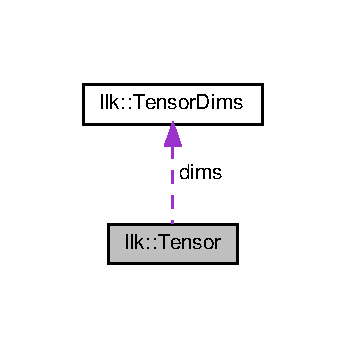
\includegraphics[width=166pt]{classllk_1_1Tensor__coll__graph}
\end{center}
\end{figure}
\subsection*{Public Member Functions}
\begin{DoxyCompactItemize}
\item 
\hyperlink{classllk_1_1Tensor_a81f468a4cb7d319155de32409bef5432}{Tensor} (int w, int z, int y, int x)
\begin{DoxyCompactList}\small\item\em Constructors -- id is optional. \end{DoxyCompactList}\item 
\hyperlink{classllk_1_1Tensor_af67761de11995474009060754829083e}{Tensor} (int w, int z, int y, int x, int \hyperlink{classllk_1_1Tensor_ae2065c91de3ad15ae38c0df9d8762f1d}{id})
\item 
\hyperlink{classllk_1_1Tensor_a4966d01a028605d769148b46de392d91}{Tensor} (int w, int z, int y, int x, int \hyperlink{classllk_1_1Tensor_ae2065c91de3ad15ae38c0df9d8762f1d}{id}, Data\+Format \hyperlink{classllk_1_1Tensor_a7a956f878f61e36905df16a6c3b043aa}{data\+\_\+format})
\item 
\hyperlink{classllk_1_1Tensor_ad86bb1c93adc9b270b066d8760838f64}{Tensor} (\hyperlink{structllk_1_1TensorDims}{Tensor\+Dims} \hyperlink{classllk_1_1Tensor_a6bad1b600bb823472f1aa770d3bbc173}{dims})
\item 
\hyperlink{classllk_1_1Tensor_a328c405eea14680ceb9dfaf56bbbd1e3}{Tensor} (\hyperlink{structllk_1_1TensorDims}{Tensor\+Dims} \hyperlink{classllk_1_1Tensor_a6bad1b600bb823472f1aa770d3bbc173}{dims}, int \hyperlink{classllk_1_1Tensor_ae2065c91de3ad15ae38c0df9d8762f1d}{id})
\item 
\hyperlink{classllk_1_1Tensor_ade260687d190ff78582a6c97e9d39445}{Tensor} (\hyperlink{structllk_1_1TensorDims}{Tensor\+Dims} \hyperlink{classllk_1_1Tensor_a6bad1b600bb823472f1aa770d3bbc173}{dims}, Data\+Format \hyperlink{classllk_1_1Tensor_a7a956f878f61e36905df16a6c3b043aa}{data\+\_\+format})
\item 
\hyperlink{classllk_1_1Tensor_ac7d05556590a616bbd1e913cefd5300a}{Tensor} (\hyperlink{structllk_1_1TensorDims}{Tensor\+Dims} \hyperlink{classllk_1_1Tensor_a6bad1b600bb823472f1aa770d3bbc173}{dims}, int \hyperlink{classllk_1_1Tensor_ae2065c91de3ad15ae38c0df9d8762f1d}{id}, Data\+Format \hyperlink{classllk_1_1Tensor_a7a956f878f61e36905df16a6c3b043aa}{data\+\_\+format})
\item 
\hyperlink{classllk_1_1Tensor_a34c1f8340785e0e96d44cb69a8f85d89}{Tensor} ()
\item 
int \hyperlink{classllk_1_1Tensor_ac55215da369eabacb7d0cd1b29d8ddab}{num\+\_\+elements} ()
\item 
int \hyperlink{classllk_1_1Tensor_acdc903190eb313866087785894a61291}{num\+\_\+tiles} ()
\item 
int \hyperlink{classllk_1_1Tensor_a021595eb6c130bffd81edfb4b39435db}{num\+\_\+bytes\+\_\+when\+\_\+assembled} ()
\item 
void \hyperlink{classllk_1_1Tensor_a17cbdfbb10299e9e9f920731376446ad}{set\+\_\+dims} (\hyperlink{structllk_1_1TensorDims}{Tensor\+Dims} \hyperlink{classllk_1_1Tensor_a6bad1b600bb823472f1aa770d3bbc173}{dims})
\item 
void \hyperlink{classllk_1_1Tensor_a6a90c8c3dae1a5e576cfc96f34586b09}{populate\+\_\+with\+\_\+debug\+\_\+data} ()
\begin{DoxyCompactList}\small\item\em Fill tensor with hardcoded data. \end{DoxyCompactList}\item 
void \hyperlink{classllk_1_1Tensor_aae7598dbef0652a4a12ee34fadc6996b}{populate\+\_\+with\+\_\+constant\+\_\+data} (float constant)
\begin{DoxyCompactList}\small\item\em Fill tensor with constant data. \end{DoxyCompactList}\item 
void \hyperlink{classllk_1_1Tensor_a72f5408bc201d59f4967169dad10b369}{populate\+\_\+with\+\_\+uniform\+\_\+distribution\+\_\+data} (float min, float max, int seed)
\begin{DoxyCompactList}\small\item\em Fill tensor with uniformly distributed data. \end{DoxyCompactList}\item 
void \hyperlink{classllk_1_1Tensor_a725baaf587a492ea43ff53356cc35fc0}{populate\+\_\+with\+\_\+normal\+\_\+distribution\+\_\+data} (float mean, float stdev, int seed)
\begin{DoxyCompactList}\small\item\em Fill tensor with normal distribution data. \end{DoxyCompactList}\item 
void \hyperlink{classllk_1_1Tensor_a17f312473d97c8786e6449236b4adf17}{reorder\+\_\+layout} (\hyperlink{namespacellk_a1cb439631a4f96e1431eea4d9b1f5cdb}{llk\+::\+Tensor\+Tile\+Layout} target\+\_\+layout)
\begin{DoxyCompactList}\small\item\em Moves the data such that it matches a different layout. \end{DoxyCompactList}\item 
void \hyperlink{classllk_1_1Tensor_a31ca8040bf822144304e7ef58fbf386f}{tilize} ()
\item 
void \hyperlink{classllk_1_1Tensor_afd6dfcbe2f92dfd0d94fb1e43f1676fb}{untilize} ()
\item 
void \hyperlink{classllk_1_1Tensor_a67d54430c95a5e279516a9470bc8f8fe}{assemble\+\_\+tiles\+\_\+to\+\_\+memory} (\hyperlink{classllk_1_1memory}{llk\+::memory} \&\hyperlink{classllk_1_1memory}{memory}, size\+\_\+t base\+\_\+address\+\_\+in\+\_\+bytes, bool aligned\+\_\+32B, \hyperlink{structllk_1_1xy__pair}{llk\+::xy\+\_\+pair} num\+\_\+blocks)
\begin{DoxyCompactList}\small\item\em Generate memory objects for each tile and assembles it together assuming row-\/major. \end{DoxyCompactList}\item 
void \hyperlink{classllk_1_1Tensor_a880292b460f36aab01d3955097af1d3e}{import\+\_\+from\+\_\+mem\+\_\+vector} (\hyperlink{structllk_1_1TensorDims}{Tensor\+Dims} \hyperlink{classllk_1_1Tensor_a6bad1b600bb823472f1aa770d3bbc173}{dims}, std\+::vector$<$ uint32\+\_\+t $>$ \&data\+\_\+vector)
\begin{DoxyCompactList}\small\item\em Reads data a mem vector. \end{DoxyCompactList}\item 
void \hyperlink{classllk_1_1Tensor_a8204b63ee3d6b146c4346fbc7727f99c}{dump} (bool to\+\_\+stdout, bool to\+\_\+file=false, std\+::string filename\+\_\+suffix=\char`\"{}\char`\"{})
\begin{DoxyCompactList}\small\item\em Dump tensor to file or to stdout. \end{DoxyCompactList}\item 
void \hyperlink{classllk_1_1Tensor_ab11ae4fa56f2ca0ba4e8f2f1670e718f}{reset\+\_\+tensor} ()
\begin{DoxyCompactList}\small\item\em Reset and zero out tensor. \end{DoxyCompactList}\end{DoxyCompactItemize}
\subsection*{Public Attributes}
\begin{DoxyCompactItemize}
\item 
int \hyperlink{classllk_1_1Tensor_ae2065c91de3ad15ae38c0df9d8762f1d}{id}
\item 
Data\+Format \hyperlink{classllk_1_1Tensor_a7a956f878f61e36905df16a6c3b043aa}{data\+\_\+format} = Data\+Format\+::\+Bfp8
\item 
\hyperlink{namespacellk_a1cb439631a4f96e1431eea4d9b1f5cdb}{llk\+::\+Tensor\+Tile\+Layout} \hyperlink{classllk_1_1Tensor_ab1d8bf151b3f9e7f6c3593937a795681}{layout} = llk\+::\+Tensor\+Tile\+Layout\+::\+R\+O\+W\+\_\+\+M\+A\+J\+OR
\item 
\hyperlink{structllk_1_1TensorDims}{llk\+::\+Tensor\+Dims} \hyperlink{classllk_1_1Tensor_a6bad1b600bb823472f1aa770d3bbc173}{dims}
\item 
bool \hyperlink{classllk_1_1Tensor_ae083a87e42384c49611eeda3c551e620}{tilized} = false
\item 
std\+::vector$<$ std\+::vector$<$ std\+::vector$<$ std\+::vector$<$ c\+\_\+tile $>$ $>$ $>$ $>$ \hyperlink{classllk_1_1Tensor_ab4e13f105e99e94bf3c10be7d0447614}{tile\+\_\+tensor}
\end{DoxyCompactItemize}


\subsection{Constructor \& Destructor Documentation}
\mbox{\Hypertarget{classllk_1_1Tensor_a81f468a4cb7d319155de32409bef5432}\label{classllk_1_1Tensor_a81f468a4cb7d319155de32409bef5432}} 
\index{llk\+::\+Tensor@{llk\+::\+Tensor}!Tensor@{Tensor}}
\index{Tensor@{Tensor}!llk\+::\+Tensor@{llk\+::\+Tensor}}
\subsubsection{\texorpdfstring{Tensor()}{Tensor()}\hspace{0.1cm}{\footnotesize\ttfamily [1/8]}}
{\footnotesize\ttfamily llk\+::\+Tensor\+::\+Tensor (\begin{DoxyParamCaption}\item[{int}]{w,  }\item[{int}]{z,  }\item[{int}]{y,  }\item[{int}]{x }\end{DoxyParamCaption})}



Constructors -- id is optional. 

\mbox{\Hypertarget{classllk_1_1Tensor_af67761de11995474009060754829083e}\label{classllk_1_1Tensor_af67761de11995474009060754829083e}} 
\index{llk\+::\+Tensor@{llk\+::\+Tensor}!Tensor@{Tensor}}
\index{Tensor@{Tensor}!llk\+::\+Tensor@{llk\+::\+Tensor}}
\subsubsection{\texorpdfstring{Tensor()}{Tensor()}\hspace{0.1cm}{\footnotesize\ttfamily [2/8]}}
{\footnotesize\ttfamily llk\+::\+Tensor\+::\+Tensor (\begin{DoxyParamCaption}\item[{int}]{w,  }\item[{int}]{z,  }\item[{int}]{y,  }\item[{int}]{x,  }\item[{int}]{id }\end{DoxyParamCaption})}

\mbox{\Hypertarget{classllk_1_1Tensor_a4966d01a028605d769148b46de392d91}\label{classllk_1_1Tensor_a4966d01a028605d769148b46de392d91}} 
\index{llk\+::\+Tensor@{llk\+::\+Tensor}!Tensor@{Tensor}}
\index{Tensor@{Tensor}!llk\+::\+Tensor@{llk\+::\+Tensor}}
\subsubsection{\texorpdfstring{Tensor()}{Tensor()}\hspace{0.1cm}{\footnotesize\ttfamily [3/8]}}
{\footnotesize\ttfamily llk\+::\+Tensor\+::\+Tensor (\begin{DoxyParamCaption}\item[{int}]{w,  }\item[{int}]{z,  }\item[{int}]{y,  }\item[{int}]{x,  }\item[{int}]{id,  }\item[{Data\+Format}]{data\+\_\+format }\end{DoxyParamCaption})}

\mbox{\Hypertarget{classllk_1_1Tensor_ad86bb1c93adc9b270b066d8760838f64}\label{classllk_1_1Tensor_ad86bb1c93adc9b270b066d8760838f64}} 
\index{llk\+::\+Tensor@{llk\+::\+Tensor}!Tensor@{Tensor}}
\index{Tensor@{Tensor}!llk\+::\+Tensor@{llk\+::\+Tensor}}
\subsubsection{\texorpdfstring{Tensor()}{Tensor()}\hspace{0.1cm}{\footnotesize\ttfamily [4/8]}}
{\footnotesize\ttfamily llk\+::\+Tensor\+::\+Tensor (\begin{DoxyParamCaption}\item[{\hyperlink{structllk_1_1TensorDims}{Tensor\+Dims}}]{dims }\end{DoxyParamCaption})}

\mbox{\Hypertarget{classllk_1_1Tensor_a328c405eea14680ceb9dfaf56bbbd1e3}\label{classllk_1_1Tensor_a328c405eea14680ceb9dfaf56bbbd1e3}} 
\index{llk\+::\+Tensor@{llk\+::\+Tensor}!Tensor@{Tensor}}
\index{Tensor@{Tensor}!llk\+::\+Tensor@{llk\+::\+Tensor}}
\subsubsection{\texorpdfstring{Tensor()}{Tensor()}\hspace{0.1cm}{\footnotesize\ttfamily [5/8]}}
{\footnotesize\ttfamily llk\+::\+Tensor\+::\+Tensor (\begin{DoxyParamCaption}\item[{\hyperlink{structllk_1_1TensorDims}{Tensor\+Dims}}]{dims,  }\item[{int}]{id }\end{DoxyParamCaption})}

\mbox{\Hypertarget{classllk_1_1Tensor_ade260687d190ff78582a6c97e9d39445}\label{classllk_1_1Tensor_ade260687d190ff78582a6c97e9d39445}} 
\index{llk\+::\+Tensor@{llk\+::\+Tensor}!Tensor@{Tensor}}
\index{Tensor@{Tensor}!llk\+::\+Tensor@{llk\+::\+Tensor}}
\subsubsection{\texorpdfstring{Tensor()}{Tensor()}\hspace{0.1cm}{\footnotesize\ttfamily [6/8]}}
{\footnotesize\ttfamily llk\+::\+Tensor\+::\+Tensor (\begin{DoxyParamCaption}\item[{\hyperlink{structllk_1_1TensorDims}{Tensor\+Dims}}]{dims,  }\item[{Data\+Format}]{data\+\_\+format }\end{DoxyParamCaption})}

\mbox{\Hypertarget{classllk_1_1Tensor_ac7d05556590a616bbd1e913cefd5300a}\label{classllk_1_1Tensor_ac7d05556590a616bbd1e913cefd5300a}} 
\index{llk\+::\+Tensor@{llk\+::\+Tensor}!Tensor@{Tensor}}
\index{Tensor@{Tensor}!llk\+::\+Tensor@{llk\+::\+Tensor}}
\subsubsection{\texorpdfstring{Tensor()}{Tensor()}\hspace{0.1cm}{\footnotesize\ttfamily [7/8]}}
{\footnotesize\ttfamily llk\+::\+Tensor\+::\+Tensor (\begin{DoxyParamCaption}\item[{\hyperlink{structllk_1_1TensorDims}{Tensor\+Dims}}]{dims,  }\item[{int}]{id,  }\item[{Data\+Format}]{data\+\_\+format }\end{DoxyParamCaption})}

\mbox{\Hypertarget{classllk_1_1Tensor_a34c1f8340785e0e96d44cb69a8f85d89}\label{classllk_1_1Tensor_a34c1f8340785e0e96d44cb69a8f85d89}} 
\index{llk\+::\+Tensor@{llk\+::\+Tensor}!Tensor@{Tensor}}
\index{Tensor@{Tensor}!llk\+::\+Tensor@{llk\+::\+Tensor}}
\subsubsection{\texorpdfstring{Tensor()}{Tensor()}\hspace{0.1cm}{\footnotesize\ttfamily [8/8]}}
{\footnotesize\ttfamily llk\+::\+Tensor\+::\+Tensor (\begin{DoxyParamCaption}{ }\end{DoxyParamCaption})}



\subsection{Member Function Documentation}
\mbox{\Hypertarget{classllk_1_1Tensor_a67d54430c95a5e279516a9470bc8f8fe}\label{classllk_1_1Tensor_a67d54430c95a5e279516a9470bc8f8fe}} 
\index{llk\+::\+Tensor@{llk\+::\+Tensor}!assemble\+\_\+tiles\+\_\+to\+\_\+memory@{assemble\+\_\+tiles\+\_\+to\+\_\+memory}}
\index{assemble\+\_\+tiles\+\_\+to\+\_\+memory@{assemble\+\_\+tiles\+\_\+to\+\_\+memory}!llk\+::\+Tensor@{llk\+::\+Tensor}}
\subsubsection{\texorpdfstring{assemble\+\_\+tiles\+\_\+to\+\_\+memory()}{assemble\_tiles\_to\_memory()}}
{\footnotesize\ttfamily void llk\+::\+Tensor\+::assemble\+\_\+tiles\+\_\+to\+\_\+memory (\begin{DoxyParamCaption}\item[{\hyperlink{classllk_1_1memory}{llk\+::memory} \&}]{memory,  }\item[{size\+\_\+t}]{base\+\_\+address\+\_\+in\+\_\+bytes,  }\item[{bool}]{aligned\+\_\+32B,  }\item[{\hyperlink{structllk_1_1xy__pair}{llk\+::xy\+\_\+pair}}]{num\+\_\+blocks }\end{DoxyParamCaption})}



Generate memory objects for each tile and assembles it together assuming row-\/major. 

\mbox{\Hypertarget{classllk_1_1Tensor_a8204b63ee3d6b146c4346fbc7727f99c}\label{classllk_1_1Tensor_a8204b63ee3d6b146c4346fbc7727f99c}} 
\index{llk\+::\+Tensor@{llk\+::\+Tensor}!dump@{dump}}
\index{dump@{dump}!llk\+::\+Tensor@{llk\+::\+Tensor}}
\subsubsection{\texorpdfstring{dump()}{dump()}}
{\footnotesize\ttfamily void llk\+::\+Tensor\+::dump (\begin{DoxyParamCaption}\item[{bool}]{to\+\_\+stdout,  }\item[{bool}]{to\+\_\+file = {\ttfamily false},  }\item[{std\+::string}]{filename\+\_\+suffix = {\ttfamily \char`\"{}\char`\"{}} }\end{DoxyParamCaption})}



Dump tensor to file or to stdout. 

\mbox{\Hypertarget{classllk_1_1Tensor_a880292b460f36aab01d3955097af1d3e}\label{classllk_1_1Tensor_a880292b460f36aab01d3955097af1d3e}} 
\index{llk\+::\+Tensor@{llk\+::\+Tensor}!import\+\_\+from\+\_\+mem\+\_\+vector@{import\+\_\+from\+\_\+mem\+\_\+vector}}
\index{import\+\_\+from\+\_\+mem\+\_\+vector@{import\+\_\+from\+\_\+mem\+\_\+vector}!llk\+::\+Tensor@{llk\+::\+Tensor}}
\subsubsection{\texorpdfstring{import\+\_\+from\+\_\+mem\+\_\+vector()}{import\_from\_mem\_vector()}}
{\footnotesize\ttfamily void llk\+::\+Tensor\+::import\+\_\+from\+\_\+mem\+\_\+vector (\begin{DoxyParamCaption}\item[{\hyperlink{structllk_1_1TensorDims}{Tensor\+Dims}}]{dims,  }\item[{std\+::vector$<$ uint32\+\_\+t $>$ \&}]{data\+\_\+vector }\end{DoxyParamCaption})}



Reads data a mem vector. 

Reads in a memory vector, assuming the tensor is set to matching format/layout already. 
\begin{DoxyParams}{Parameters}
{\em dims} & dimensions of the tensor to interpret from vector. \\
\hline
{\em data\+\_\+vector} & the vector to read data from. assumes it is tightly packed and has headers \\
\hline
\end{DoxyParams}
\mbox{\Hypertarget{classllk_1_1Tensor_a021595eb6c130bffd81edfb4b39435db}\label{classllk_1_1Tensor_a021595eb6c130bffd81edfb4b39435db}} 
\index{llk\+::\+Tensor@{llk\+::\+Tensor}!num\+\_\+bytes\+\_\+when\+\_\+assembled@{num\+\_\+bytes\+\_\+when\+\_\+assembled}}
\index{num\+\_\+bytes\+\_\+when\+\_\+assembled@{num\+\_\+bytes\+\_\+when\+\_\+assembled}!llk\+::\+Tensor@{llk\+::\+Tensor}}
\subsubsection{\texorpdfstring{num\+\_\+bytes\+\_\+when\+\_\+assembled()}{num\_bytes\_when\_assembled()}}
{\footnotesize\ttfamily int llk\+::\+Tensor\+::num\+\_\+bytes\+\_\+when\+\_\+assembled (\begin{DoxyParamCaption}{ }\end{DoxyParamCaption})\hspace{0.3cm}{\ttfamily [inline]}}

\mbox{\Hypertarget{classllk_1_1Tensor_ac55215da369eabacb7d0cd1b29d8ddab}\label{classllk_1_1Tensor_ac55215da369eabacb7d0cd1b29d8ddab}} 
\index{llk\+::\+Tensor@{llk\+::\+Tensor}!num\+\_\+elements@{num\+\_\+elements}}
\index{num\+\_\+elements@{num\+\_\+elements}!llk\+::\+Tensor@{llk\+::\+Tensor}}
\subsubsection{\texorpdfstring{num\+\_\+elements()}{num\_elements()}}
{\footnotesize\ttfamily int llk\+::\+Tensor\+::num\+\_\+elements (\begin{DoxyParamCaption}{ }\end{DoxyParamCaption})\hspace{0.3cm}{\ttfamily [inline]}}

\mbox{\Hypertarget{classllk_1_1Tensor_acdc903190eb313866087785894a61291}\label{classllk_1_1Tensor_acdc903190eb313866087785894a61291}} 
\index{llk\+::\+Tensor@{llk\+::\+Tensor}!num\+\_\+tiles@{num\+\_\+tiles}}
\index{num\+\_\+tiles@{num\+\_\+tiles}!llk\+::\+Tensor@{llk\+::\+Tensor}}
\subsubsection{\texorpdfstring{num\+\_\+tiles()}{num\_tiles()}}
{\footnotesize\ttfamily int llk\+::\+Tensor\+::num\+\_\+tiles (\begin{DoxyParamCaption}{ }\end{DoxyParamCaption})\hspace{0.3cm}{\ttfamily [inline]}}

\mbox{\Hypertarget{classllk_1_1Tensor_aae7598dbef0652a4a12ee34fadc6996b}\label{classllk_1_1Tensor_aae7598dbef0652a4a12ee34fadc6996b}} 
\index{llk\+::\+Tensor@{llk\+::\+Tensor}!populate\+\_\+with\+\_\+constant\+\_\+data@{populate\+\_\+with\+\_\+constant\+\_\+data}}
\index{populate\+\_\+with\+\_\+constant\+\_\+data@{populate\+\_\+with\+\_\+constant\+\_\+data}!llk\+::\+Tensor@{llk\+::\+Tensor}}
\subsubsection{\texorpdfstring{populate\+\_\+with\+\_\+constant\+\_\+data()}{populate\_with\_constant\_data()}}
{\footnotesize\ttfamily void llk\+::\+Tensor\+::populate\+\_\+with\+\_\+constant\+\_\+data (\begin{DoxyParamCaption}\item[{float}]{constant }\end{DoxyParamCaption})}



Fill tensor with constant data. 

\mbox{\Hypertarget{classllk_1_1Tensor_a6a90c8c3dae1a5e576cfc96f34586b09}\label{classllk_1_1Tensor_a6a90c8c3dae1a5e576cfc96f34586b09}} 
\index{llk\+::\+Tensor@{llk\+::\+Tensor}!populate\+\_\+with\+\_\+debug\+\_\+data@{populate\+\_\+with\+\_\+debug\+\_\+data}}
\index{populate\+\_\+with\+\_\+debug\+\_\+data@{populate\+\_\+with\+\_\+debug\+\_\+data}!llk\+::\+Tensor@{llk\+::\+Tensor}}
\subsubsection{\texorpdfstring{populate\+\_\+with\+\_\+debug\+\_\+data()}{populate\_with\_debug\_data()}}
{\footnotesize\ttfamily void llk\+::\+Tensor\+::populate\+\_\+with\+\_\+debug\+\_\+data (\begin{DoxyParamCaption}{ }\end{DoxyParamCaption})}



Fill tensor with hardcoded data. 

\mbox{\Hypertarget{classllk_1_1Tensor_a725baaf587a492ea43ff53356cc35fc0}\label{classllk_1_1Tensor_a725baaf587a492ea43ff53356cc35fc0}} 
\index{llk\+::\+Tensor@{llk\+::\+Tensor}!populate\+\_\+with\+\_\+normal\+\_\+distribution\+\_\+data@{populate\+\_\+with\+\_\+normal\+\_\+distribution\+\_\+data}}
\index{populate\+\_\+with\+\_\+normal\+\_\+distribution\+\_\+data@{populate\+\_\+with\+\_\+normal\+\_\+distribution\+\_\+data}!llk\+::\+Tensor@{llk\+::\+Tensor}}
\subsubsection{\texorpdfstring{populate\+\_\+with\+\_\+normal\+\_\+distribution\+\_\+data()}{populate\_with\_normal\_distribution\_data()}}
{\footnotesize\ttfamily void llk\+::\+Tensor\+::populate\+\_\+with\+\_\+normal\+\_\+distribution\+\_\+data (\begin{DoxyParamCaption}\item[{float}]{mean,  }\item[{float}]{stdev,  }\item[{int}]{seed }\end{DoxyParamCaption})}



Fill tensor with normal distribution data. 

\mbox{\Hypertarget{classllk_1_1Tensor_a72f5408bc201d59f4967169dad10b369}\label{classllk_1_1Tensor_a72f5408bc201d59f4967169dad10b369}} 
\index{llk\+::\+Tensor@{llk\+::\+Tensor}!populate\+\_\+with\+\_\+uniform\+\_\+distribution\+\_\+data@{populate\+\_\+with\+\_\+uniform\+\_\+distribution\+\_\+data}}
\index{populate\+\_\+with\+\_\+uniform\+\_\+distribution\+\_\+data@{populate\+\_\+with\+\_\+uniform\+\_\+distribution\+\_\+data}!llk\+::\+Tensor@{llk\+::\+Tensor}}
\subsubsection{\texorpdfstring{populate\+\_\+with\+\_\+uniform\+\_\+distribution\+\_\+data()}{populate\_with\_uniform\_distribution\_data()}}
{\footnotesize\ttfamily void llk\+::\+Tensor\+::populate\+\_\+with\+\_\+uniform\+\_\+distribution\+\_\+data (\begin{DoxyParamCaption}\item[{float}]{min,  }\item[{float}]{max,  }\item[{int}]{seed }\end{DoxyParamCaption})}



Fill tensor with uniformly distributed data. 

\mbox{\Hypertarget{classllk_1_1Tensor_a17f312473d97c8786e6449236b4adf17}\label{classllk_1_1Tensor_a17f312473d97c8786e6449236b4adf17}} 
\index{llk\+::\+Tensor@{llk\+::\+Tensor}!reorder\+\_\+layout@{reorder\+\_\+layout}}
\index{reorder\+\_\+layout@{reorder\+\_\+layout}!llk\+::\+Tensor@{llk\+::\+Tensor}}
\subsubsection{\texorpdfstring{reorder\+\_\+layout()}{reorder\_layout()}}
{\footnotesize\ttfamily void llk\+::\+Tensor\+::reorder\+\_\+layout (\begin{DoxyParamCaption}\item[{\hyperlink{namespacellk_a1cb439631a4f96e1431eea4d9b1f5cdb}{llk\+::\+Tensor\+Tile\+Layout}}]{target\+\_\+layout }\end{DoxyParamCaption})}



Moves the data such that it matches a different layout. 

\mbox{\Hypertarget{classllk_1_1Tensor_ab11ae4fa56f2ca0ba4e8f2f1670e718f}\label{classllk_1_1Tensor_ab11ae4fa56f2ca0ba4e8f2f1670e718f}} 
\index{llk\+::\+Tensor@{llk\+::\+Tensor}!reset\+\_\+tensor@{reset\+\_\+tensor}}
\index{reset\+\_\+tensor@{reset\+\_\+tensor}!llk\+::\+Tensor@{llk\+::\+Tensor}}
\subsubsection{\texorpdfstring{reset\+\_\+tensor()}{reset\_tensor()}}
{\footnotesize\ttfamily void llk\+::\+Tensor\+::reset\+\_\+tensor (\begin{DoxyParamCaption}{ }\end{DoxyParamCaption})}



Reset and zero out tensor. 

\mbox{\Hypertarget{classllk_1_1Tensor_a17cbdfbb10299e9e9f920731376446ad}\label{classllk_1_1Tensor_a17cbdfbb10299e9e9f920731376446ad}} 
\index{llk\+::\+Tensor@{llk\+::\+Tensor}!set\+\_\+dims@{set\+\_\+dims}}
\index{set\+\_\+dims@{set\+\_\+dims}!llk\+::\+Tensor@{llk\+::\+Tensor}}
\subsubsection{\texorpdfstring{set\+\_\+dims()}{set\_dims()}}
{\footnotesize\ttfamily void llk\+::\+Tensor\+::set\+\_\+dims (\begin{DoxyParamCaption}\item[{\hyperlink{structllk_1_1TensorDims}{Tensor\+Dims}}]{dims }\end{DoxyParamCaption})}

\mbox{\Hypertarget{classllk_1_1Tensor_a31ca8040bf822144304e7ef58fbf386f}\label{classllk_1_1Tensor_a31ca8040bf822144304e7ef58fbf386f}} 
\index{llk\+::\+Tensor@{llk\+::\+Tensor}!tilize@{tilize}}
\index{tilize@{tilize}!llk\+::\+Tensor@{llk\+::\+Tensor}}
\subsubsection{\texorpdfstring{tilize()}{tilize()}}
{\footnotesize\ttfamily void llk\+::\+Tensor\+::tilize (\begin{DoxyParamCaption}{ }\end{DoxyParamCaption})}

\mbox{\Hypertarget{classllk_1_1Tensor_afd6dfcbe2f92dfd0d94fb1e43f1676fb}\label{classllk_1_1Tensor_afd6dfcbe2f92dfd0d94fb1e43f1676fb}} 
\index{llk\+::\+Tensor@{llk\+::\+Tensor}!untilize@{untilize}}
\index{untilize@{untilize}!llk\+::\+Tensor@{llk\+::\+Tensor}}
\subsubsection{\texorpdfstring{untilize()}{untilize()}}
{\footnotesize\ttfamily void llk\+::\+Tensor\+::untilize (\begin{DoxyParamCaption}{ }\end{DoxyParamCaption})}



\subsection{Member Data Documentation}
\mbox{\Hypertarget{classllk_1_1Tensor_a7a956f878f61e36905df16a6c3b043aa}\label{classllk_1_1Tensor_a7a956f878f61e36905df16a6c3b043aa}} 
\index{llk\+::\+Tensor@{llk\+::\+Tensor}!data\+\_\+format@{data\+\_\+format}}
\index{data\+\_\+format@{data\+\_\+format}!llk\+::\+Tensor@{llk\+::\+Tensor}}
\subsubsection{\texorpdfstring{data\+\_\+format}{data\_format}}
{\footnotesize\ttfamily Data\+Format llk\+::\+Tensor\+::data\+\_\+format = Data\+Format\+::\+Bfp8}

\mbox{\Hypertarget{classllk_1_1Tensor_a6bad1b600bb823472f1aa770d3bbc173}\label{classllk_1_1Tensor_a6bad1b600bb823472f1aa770d3bbc173}} 
\index{llk\+::\+Tensor@{llk\+::\+Tensor}!dims@{dims}}
\index{dims@{dims}!llk\+::\+Tensor@{llk\+::\+Tensor}}
\subsubsection{\texorpdfstring{dims}{dims}}
{\footnotesize\ttfamily \hyperlink{structllk_1_1TensorDims}{llk\+::\+Tensor\+Dims} llk\+::\+Tensor\+::dims}

\mbox{\Hypertarget{classllk_1_1Tensor_ae2065c91de3ad15ae38c0df9d8762f1d}\label{classllk_1_1Tensor_ae2065c91de3ad15ae38c0df9d8762f1d}} 
\index{llk\+::\+Tensor@{llk\+::\+Tensor}!id@{id}}
\index{id@{id}!llk\+::\+Tensor@{llk\+::\+Tensor}}
\subsubsection{\texorpdfstring{id}{id}}
{\footnotesize\ttfamily int llk\+::\+Tensor\+::id}

\mbox{\Hypertarget{classllk_1_1Tensor_ab1d8bf151b3f9e7f6c3593937a795681}\label{classllk_1_1Tensor_ab1d8bf151b3f9e7f6c3593937a795681}} 
\index{llk\+::\+Tensor@{llk\+::\+Tensor}!layout@{layout}}
\index{layout@{layout}!llk\+::\+Tensor@{llk\+::\+Tensor}}
\subsubsection{\texorpdfstring{layout}{layout}}
{\footnotesize\ttfamily \hyperlink{namespacellk_a1cb439631a4f96e1431eea4d9b1f5cdb}{llk\+::\+Tensor\+Tile\+Layout} llk\+::\+Tensor\+::layout = llk\+::\+Tensor\+Tile\+Layout\+::\+R\+O\+W\+\_\+\+M\+A\+J\+OR}

\mbox{\Hypertarget{classllk_1_1Tensor_ab4e13f105e99e94bf3c10be7d0447614}\label{classllk_1_1Tensor_ab4e13f105e99e94bf3c10be7d0447614}} 
\index{llk\+::\+Tensor@{llk\+::\+Tensor}!tile\+\_\+tensor@{tile\+\_\+tensor}}
\index{tile\+\_\+tensor@{tile\+\_\+tensor}!llk\+::\+Tensor@{llk\+::\+Tensor}}
\subsubsection{\texorpdfstring{tile\+\_\+tensor}{tile\_tensor}}
{\footnotesize\ttfamily std\+::vector$<$std\+::vector$<$std\+::vector$<$std\+::vector$<$c\+\_\+tile$>$ $>$ $>$ $>$ llk\+::\+Tensor\+::tile\+\_\+tensor}

\mbox{\Hypertarget{classllk_1_1Tensor_ae083a87e42384c49611eeda3c551e620}\label{classllk_1_1Tensor_ae083a87e42384c49611eeda3c551e620}} 
\index{llk\+::\+Tensor@{llk\+::\+Tensor}!tilized@{tilized}}
\index{tilized@{tilized}!llk\+::\+Tensor@{llk\+::\+Tensor}}
\subsubsection{\texorpdfstring{tilized}{tilized}}
{\footnotesize\ttfamily bool llk\+::\+Tensor\+::tilized = false}



The documentation for this class was generated from the following files\+:\begin{DoxyCompactItemize}
\item 
inc/\hyperlink{llk__tensor_8h}{llk\+\_\+tensor.\+h}\item 
src/\hyperlink{llk__tensor_8cpp}{llk\+\_\+tensor.\+cpp}\end{DoxyCompactItemize}

\hypertarget{structtests_1_1TensorConfig}{}\section{tests\+:\+:Tensor\+Config Struct Reference}
\label{structtests_1_1TensorConfig}\index{tests\+::\+Tensor\+Config@{tests\+::\+Tensor\+Config}}


{\ttfamily \#include $<$test\+\_\+tensor\+\_\+config.\+h$>$}



Collaboration diagram for tests\+:\+:Tensor\+Config\+:\nopagebreak
\begin{figure}[H]
\begin{center}
\leavevmode
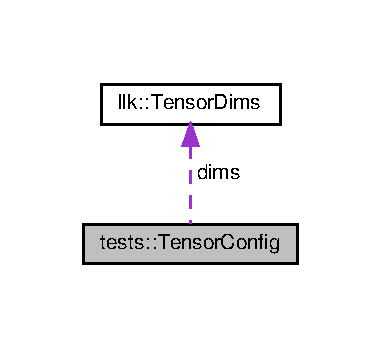
\includegraphics[width=183pt]{structtests_1_1TensorConfig__coll__graph}
\end{center}
\end{figure}
\subsection*{Public Member Functions}
\begin{DoxyCompactItemize}
\item 
\hyperlink{structtests_1_1TensorConfig_ac5ddc9579a693945b75a943441e28cf1}{Tensor\+Config} ()
\item 
\hyperlink{structtests_1_1TensorConfig_a10b3a5e1299b4a687021d4442cf8a611}{Tensor\+Config} (\hyperlink{structllk_1_1TensorDims}{llk\+::\+Tensor\+Dims} \hyperlink{structtests_1_1TensorConfig_a7b27f127ff4b7a04694dfad1d7500244}{dims}, Data\+Format \hyperlink{structtests_1_1TensorConfig_a53af0a893eebf1329c848818dcea1a08}{data\+\_\+format})
\end{DoxyCompactItemize}
\subsection*{Public Attributes}
\begin{DoxyCompactItemize}
\item 
\hyperlink{structllk_1_1TensorDims}{llk\+::\+Tensor\+Dims} \hyperlink{structtests_1_1TensorConfig_a7b27f127ff4b7a04694dfad1d7500244}{dims} = \{\}
\item 
Data\+Format \hyperlink{structtests_1_1TensorConfig_a53af0a893eebf1329c848818dcea1a08}{data\+\_\+format}
\item 
map$<$ string, string $>$ \hyperlink{structtests_1_1TensorConfig_a05d85214444feab610a4e4752f51d176}{stimulus\+\_\+config}
\end{DoxyCompactItemize}


\subsection{Constructor \& Destructor Documentation}
\mbox{\Hypertarget{structtests_1_1TensorConfig_ac5ddc9579a693945b75a943441e28cf1}\label{structtests_1_1TensorConfig_ac5ddc9579a693945b75a943441e28cf1}} 
\index{tests\+::\+Tensor\+Config@{tests\+::\+Tensor\+Config}!Tensor\+Config@{Tensor\+Config}}
\index{Tensor\+Config@{Tensor\+Config}!tests\+::\+Tensor\+Config@{tests\+::\+Tensor\+Config}}
\subsubsection{\texorpdfstring{Tensor\+Config()}{TensorConfig()}\hspace{0.1cm}{\footnotesize\ttfamily [1/2]}}
{\footnotesize\ttfamily tests\+::\+Tensor\+Config\+::\+Tensor\+Config (\begin{DoxyParamCaption}{ }\end{DoxyParamCaption})}

\mbox{\Hypertarget{structtests_1_1TensorConfig_a10b3a5e1299b4a687021d4442cf8a611}\label{structtests_1_1TensorConfig_a10b3a5e1299b4a687021d4442cf8a611}} 
\index{tests\+::\+Tensor\+Config@{tests\+::\+Tensor\+Config}!Tensor\+Config@{Tensor\+Config}}
\index{Tensor\+Config@{Tensor\+Config}!tests\+::\+Tensor\+Config@{tests\+::\+Tensor\+Config}}
\subsubsection{\texorpdfstring{Tensor\+Config()}{TensorConfig()}\hspace{0.1cm}{\footnotesize\ttfamily [2/2]}}
{\footnotesize\ttfamily tests\+::\+Tensor\+Config\+::\+Tensor\+Config (\begin{DoxyParamCaption}\item[{\hyperlink{structllk_1_1TensorDims}{llk\+::\+Tensor\+Dims}}]{dims,  }\item[{Data\+Format}]{data\+\_\+format }\end{DoxyParamCaption})}



\subsection{Member Data Documentation}
\mbox{\Hypertarget{structtests_1_1TensorConfig_a53af0a893eebf1329c848818dcea1a08}\label{structtests_1_1TensorConfig_a53af0a893eebf1329c848818dcea1a08}} 
\index{tests\+::\+Tensor\+Config@{tests\+::\+Tensor\+Config}!data\+\_\+format@{data\+\_\+format}}
\index{data\+\_\+format@{data\+\_\+format}!tests\+::\+Tensor\+Config@{tests\+::\+Tensor\+Config}}
\subsubsection{\texorpdfstring{data\+\_\+format}{data\_format}}
{\footnotesize\ttfamily Data\+Format tests\+::\+Tensor\+Config\+::data\+\_\+format}

\mbox{\Hypertarget{structtests_1_1TensorConfig_a7b27f127ff4b7a04694dfad1d7500244}\label{structtests_1_1TensorConfig_a7b27f127ff4b7a04694dfad1d7500244}} 
\index{tests\+::\+Tensor\+Config@{tests\+::\+Tensor\+Config}!dims@{dims}}
\index{dims@{dims}!tests\+::\+Tensor\+Config@{tests\+::\+Tensor\+Config}}
\subsubsection{\texorpdfstring{dims}{dims}}
{\footnotesize\ttfamily \hyperlink{structllk_1_1TensorDims}{llk\+::\+Tensor\+Dims} tests\+::\+Tensor\+Config\+::dims = \{\}}

\mbox{\Hypertarget{structtests_1_1TensorConfig_a05d85214444feab610a4e4752f51d176}\label{structtests_1_1TensorConfig_a05d85214444feab610a4e4752f51d176}} 
\index{tests\+::\+Tensor\+Config@{tests\+::\+Tensor\+Config}!stimulus\+\_\+config@{stimulus\+\_\+config}}
\index{stimulus\+\_\+config@{stimulus\+\_\+config}!tests\+::\+Tensor\+Config@{tests\+::\+Tensor\+Config}}
\subsubsection{\texorpdfstring{stimulus\+\_\+config}{stimulus\_config}}
{\footnotesize\ttfamily map$<$string, string$>$ tests\+::\+Tensor\+Config\+::stimulus\+\_\+config}



The documentation for this struct was generated from the following files\+:\begin{DoxyCompactItemize}
\item 
tests/\hyperlink{test__tensor__config_8h}{test\+\_\+tensor\+\_\+config.\+h}\item 
tests/\hyperlink{test__tensor__config_8cpp}{test\+\_\+tensor\+\_\+config.\+cpp}\end{DoxyCompactItemize}

\hypertarget{structllk_1_1TensorDims}{}\section{llk\+:\+:Tensor\+Dims Struct Reference}
\label{structllk_1_1TensorDims}\index{llk\+::\+Tensor\+Dims@{llk\+::\+Tensor\+Dims}}


{\ttfamily \#include $<$llk\+\_\+tensor\+\_\+dims.\+h$>$}

\subsection*{Public Member Functions}
\begin{DoxyCompactItemize}
\item 
\hyperlink{structllk_1_1TensorDims_a5bc2a28dad2022e94da65c139a49af41}{Tensor\+Dims} (int \hyperlink{structllk_1_1TensorDims_aaf0debf1e0ce1dedcd4827b14404747e}{w}, int \hyperlink{structllk_1_1TensorDims_a9c66eaf5cab067403864bfec44d10dc1}{z}, int \hyperlink{structllk_1_1TensorDims_afabf2a6cb993733866a5127bd5c8054b}{y}, int \hyperlink{structllk_1_1TensorDims_a06e23d03e9701fb0cd42109c2c89e14f}{x})
\item 
\hyperlink{structllk_1_1TensorDims_a274790cfc2358a8e5a0eedeb9c1f561a}{Tensor\+Dims} (std\+::vector$<$ int $>$ dims)
\item 
\hyperlink{structllk_1_1TensorDims_a89958061a8264d7e255b651a71ed5320}{Tensor\+Dims} ()
\item 
bool \hyperlink{structllk_1_1TensorDims_afa299058bf3c824a463505b32ed69cfe}{equal} (const \hyperlink{structllk_1_1TensorDims}{llk\+::\+Tensor\+Dims} \&rh)
\item 
int \hyperlink{structllk_1_1TensorDims_aedcddc34ae754148de0d2c7ae4bc74a5}{num\+\_\+tiles} ()
\item 
int \hyperlink{structllk_1_1TensorDims_a9197175910b011a4f4d5ca3ab0cd9194}{tile\+\_\+bytes\+\_\+when\+\_\+assembled} (Data\+Format format)
\item 
int \hyperlink{structllk_1_1TensorDims_a36b6a517cf22124b0416a5049497aac6}{num\+\_\+bytes\+\_\+when\+\_\+assembled} (Data\+Format format)
\item 
bool \hyperlink{structllk_1_1TensorDims_afd06417a99310c75f8a997de33ca34a6}{operator==} (\hyperlink{structllk_1_1TensorDims}{llk\+::\+Tensor\+Dims} \&rh)
\item 
bool \hyperlink{structllk_1_1TensorDims_ad4d5bb7fe50f517c3d8114d907d77245}{operator!=} (\hyperlink{structllk_1_1TensorDims}{llk\+::\+Tensor\+Dims} \&rh)
\item 
int \hyperlink{structllk_1_1TensorDims_abc98fc97e0628bbc001e890bd2006341}{num\+\_\+elements} ()
\item 
int \hyperlink{structllk_1_1TensorDims_a891fb5dd7544fa99494bb496e2e4491b}{num\+\_\+elements\+\_\+per\+\_\+tile} ()
\item 
std\+::string \hyperlink{structllk_1_1TensorDims_aba8753250cc5a9643776e29c9279a431}{str} () const
\end{DoxyCompactItemize}
\subsection*{Public Attributes}
\begin{DoxyCompactItemize}
\item 
int \hyperlink{structllk_1_1TensorDims_abed7f5a8a79ea929142ad1a2fba6752d}{rt}
\item 
int \hyperlink{structllk_1_1TensorDims_a61f71e8dcc5b6bba20cfc89b4f7e899c}{ct}
\item 
int \hyperlink{structllk_1_1TensorDims_a06e23d03e9701fb0cd42109c2c89e14f}{x}
\item 
int \hyperlink{structllk_1_1TensorDims_afabf2a6cb993733866a5127bd5c8054b}{y}
\item 
int \hyperlink{structllk_1_1TensorDims_a9c66eaf5cab067403864bfec44d10dc1}{z}
\item 
int \hyperlink{structllk_1_1TensorDims_aaf0debf1e0ce1dedcd4827b14404747e}{w}
\end{DoxyCompactItemize}
\subsection*{Static Public Attributes}
\begin{DoxyCompactItemize}
\item 
static constexpr size\+\_\+t \hyperlink{structllk_1_1TensorDims_ae4a0ec57dc566e3c3b3fe0a932a41b4f}{T\+I\+L\+E\+\_\+\+R\+O\+W\+\_\+\+D\+IM} = 32
\item 
static constexpr size\+\_\+t \hyperlink{structllk_1_1TensorDims_a812883e0fbbbb1e47630c2eae55ebd7d}{T\+I\+L\+E\+\_\+\+C\+O\+L\+\_\+\+D\+IM} = 32
\end{DoxyCompactItemize}


\subsection{Constructor \& Destructor Documentation}
\mbox{\Hypertarget{structllk_1_1TensorDims_a5bc2a28dad2022e94da65c139a49af41}\label{structllk_1_1TensorDims_a5bc2a28dad2022e94da65c139a49af41}} 
\index{llk\+::\+Tensor\+Dims@{llk\+::\+Tensor\+Dims}!Tensor\+Dims@{Tensor\+Dims}}
\index{Tensor\+Dims@{Tensor\+Dims}!llk\+::\+Tensor\+Dims@{llk\+::\+Tensor\+Dims}}
\subsubsection{\texorpdfstring{Tensor\+Dims()}{TensorDims()}\hspace{0.1cm}{\footnotesize\ttfamily [1/3]}}
{\footnotesize\ttfamily llk\+::\+Tensor\+Dims\+::\+Tensor\+Dims (\begin{DoxyParamCaption}\item[{int}]{w,  }\item[{int}]{z,  }\item[{int}]{y,  }\item[{int}]{x }\end{DoxyParamCaption})\hspace{0.3cm}{\ttfamily [inline]}}

\mbox{\Hypertarget{structllk_1_1TensorDims_a274790cfc2358a8e5a0eedeb9c1f561a}\label{structllk_1_1TensorDims_a274790cfc2358a8e5a0eedeb9c1f561a}} 
\index{llk\+::\+Tensor\+Dims@{llk\+::\+Tensor\+Dims}!Tensor\+Dims@{Tensor\+Dims}}
\index{Tensor\+Dims@{Tensor\+Dims}!llk\+::\+Tensor\+Dims@{llk\+::\+Tensor\+Dims}}
\subsubsection{\texorpdfstring{Tensor\+Dims()}{TensorDims()}\hspace{0.1cm}{\footnotesize\ttfamily [2/3]}}
{\footnotesize\ttfamily llk\+::\+Tensor\+Dims\+::\+Tensor\+Dims (\begin{DoxyParamCaption}\item[{std\+::vector$<$ int $>$}]{dims }\end{DoxyParamCaption})\hspace{0.3cm}{\ttfamily [inline]}}

\mbox{\Hypertarget{structllk_1_1TensorDims_a89958061a8264d7e255b651a71ed5320}\label{structllk_1_1TensorDims_a89958061a8264d7e255b651a71ed5320}} 
\index{llk\+::\+Tensor\+Dims@{llk\+::\+Tensor\+Dims}!Tensor\+Dims@{Tensor\+Dims}}
\index{Tensor\+Dims@{Tensor\+Dims}!llk\+::\+Tensor\+Dims@{llk\+::\+Tensor\+Dims}}
\subsubsection{\texorpdfstring{Tensor\+Dims()}{TensorDims()}\hspace{0.1cm}{\footnotesize\ttfamily [3/3]}}
{\footnotesize\ttfamily llk\+::\+Tensor\+Dims\+::\+Tensor\+Dims (\begin{DoxyParamCaption}{ }\end{DoxyParamCaption})\hspace{0.3cm}{\ttfamily [inline]}}



\subsection{Member Function Documentation}
\mbox{\Hypertarget{structllk_1_1TensorDims_afa299058bf3c824a463505b32ed69cfe}\label{structllk_1_1TensorDims_afa299058bf3c824a463505b32ed69cfe}} 
\index{llk\+::\+Tensor\+Dims@{llk\+::\+Tensor\+Dims}!equal@{equal}}
\index{equal@{equal}!llk\+::\+Tensor\+Dims@{llk\+::\+Tensor\+Dims}}
\subsubsection{\texorpdfstring{equal()}{equal()}}
{\footnotesize\ttfamily bool llk\+::\+Tensor\+Dims\+::equal (\begin{DoxyParamCaption}\item[{const \hyperlink{structllk_1_1TensorDims}{llk\+::\+Tensor\+Dims} \&}]{rh }\end{DoxyParamCaption})\hspace{0.3cm}{\ttfamily [inline]}}

\mbox{\Hypertarget{structllk_1_1TensorDims_a36b6a517cf22124b0416a5049497aac6}\label{structllk_1_1TensorDims_a36b6a517cf22124b0416a5049497aac6}} 
\index{llk\+::\+Tensor\+Dims@{llk\+::\+Tensor\+Dims}!num\+\_\+bytes\+\_\+when\+\_\+assembled@{num\+\_\+bytes\+\_\+when\+\_\+assembled}}
\index{num\+\_\+bytes\+\_\+when\+\_\+assembled@{num\+\_\+bytes\+\_\+when\+\_\+assembled}!llk\+::\+Tensor\+Dims@{llk\+::\+Tensor\+Dims}}
\subsubsection{\texorpdfstring{num\+\_\+bytes\+\_\+when\+\_\+assembled()}{num\_bytes\_when\_assembled()}}
{\footnotesize\ttfamily int llk\+::\+Tensor\+Dims\+::num\+\_\+bytes\+\_\+when\+\_\+assembled (\begin{DoxyParamCaption}\item[{Data\+Format}]{format }\end{DoxyParamCaption})\hspace{0.3cm}{\ttfamily [inline]}}

\mbox{\Hypertarget{structllk_1_1TensorDims_abc98fc97e0628bbc001e890bd2006341}\label{structllk_1_1TensorDims_abc98fc97e0628bbc001e890bd2006341}} 
\index{llk\+::\+Tensor\+Dims@{llk\+::\+Tensor\+Dims}!num\+\_\+elements@{num\+\_\+elements}}
\index{num\+\_\+elements@{num\+\_\+elements}!llk\+::\+Tensor\+Dims@{llk\+::\+Tensor\+Dims}}
\subsubsection{\texorpdfstring{num\+\_\+elements()}{num\_elements()}}
{\footnotesize\ttfamily int llk\+::\+Tensor\+Dims\+::num\+\_\+elements (\begin{DoxyParamCaption}{ }\end{DoxyParamCaption})\hspace{0.3cm}{\ttfamily [inline]}}

\mbox{\Hypertarget{structllk_1_1TensorDims_a891fb5dd7544fa99494bb496e2e4491b}\label{structllk_1_1TensorDims_a891fb5dd7544fa99494bb496e2e4491b}} 
\index{llk\+::\+Tensor\+Dims@{llk\+::\+Tensor\+Dims}!num\+\_\+elements\+\_\+per\+\_\+tile@{num\+\_\+elements\+\_\+per\+\_\+tile}}
\index{num\+\_\+elements\+\_\+per\+\_\+tile@{num\+\_\+elements\+\_\+per\+\_\+tile}!llk\+::\+Tensor\+Dims@{llk\+::\+Tensor\+Dims}}
\subsubsection{\texorpdfstring{num\+\_\+elements\+\_\+per\+\_\+tile()}{num\_elements\_per\_tile()}}
{\footnotesize\ttfamily int llk\+::\+Tensor\+Dims\+::num\+\_\+elements\+\_\+per\+\_\+tile (\begin{DoxyParamCaption}{ }\end{DoxyParamCaption})\hspace{0.3cm}{\ttfamily [inline]}}

\mbox{\Hypertarget{structllk_1_1TensorDims_aedcddc34ae754148de0d2c7ae4bc74a5}\label{structllk_1_1TensorDims_aedcddc34ae754148de0d2c7ae4bc74a5}} 
\index{llk\+::\+Tensor\+Dims@{llk\+::\+Tensor\+Dims}!num\+\_\+tiles@{num\+\_\+tiles}}
\index{num\+\_\+tiles@{num\+\_\+tiles}!llk\+::\+Tensor\+Dims@{llk\+::\+Tensor\+Dims}}
\subsubsection{\texorpdfstring{num\+\_\+tiles()}{num\_tiles()}}
{\footnotesize\ttfamily int llk\+::\+Tensor\+Dims\+::num\+\_\+tiles (\begin{DoxyParamCaption}{ }\end{DoxyParamCaption})\hspace{0.3cm}{\ttfamily [inline]}}

\mbox{\Hypertarget{structllk_1_1TensorDims_ad4d5bb7fe50f517c3d8114d907d77245}\label{structllk_1_1TensorDims_ad4d5bb7fe50f517c3d8114d907d77245}} 
\index{llk\+::\+Tensor\+Dims@{llk\+::\+Tensor\+Dims}!operator"!=@{operator"!=}}
\index{operator"!=@{operator"!=}!llk\+::\+Tensor\+Dims@{llk\+::\+Tensor\+Dims}}
\subsubsection{\texorpdfstring{operator"!=()}{operator!=()}}
{\footnotesize\ttfamily bool llk\+::\+Tensor\+Dims\+::operator!= (\begin{DoxyParamCaption}\item[{\hyperlink{structllk_1_1TensorDims}{llk\+::\+Tensor\+Dims} \&}]{rh }\end{DoxyParamCaption})\hspace{0.3cm}{\ttfamily [inline]}}

\mbox{\Hypertarget{structllk_1_1TensorDims_afd06417a99310c75f8a997de33ca34a6}\label{structllk_1_1TensorDims_afd06417a99310c75f8a997de33ca34a6}} 
\index{llk\+::\+Tensor\+Dims@{llk\+::\+Tensor\+Dims}!operator==@{operator==}}
\index{operator==@{operator==}!llk\+::\+Tensor\+Dims@{llk\+::\+Tensor\+Dims}}
\subsubsection{\texorpdfstring{operator==()}{operator==()}}
{\footnotesize\ttfamily bool llk\+::\+Tensor\+Dims\+::operator== (\begin{DoxyParamCaption}\item[{\hyperlink{structllk_1_1TensorDims}{llk\+::\+Tensor\+Dims} \&}]{rh }\end{DoxyParamCaption})\hspace{0.3cm}{\ttfamily [inline]}}

\mbox{\Hypertarget{structllk_1_1TensorDims_aba8753250cc5a9643776e29c9279a431}\label{structllk_1_1TensorDims_aba8753250cc5a9643776e29c9279a431}} 
\index{llk\+::\+Tensor\+Dims@{llk\+::\+Tensor\+Dims}!str@{str}}
\index{str@{str}!llk\+::\+Tensor\+Dims@{llk\+::\+Tensor\+Dims}}
\subsubsection{\texorpdfstring{str()}{str()}}
{\footnotesize\ttfamily std\+::string llk\+::\+Tensor\+Dims\+::str (\begin{DoxyParamCaption}{ }\end{DoxyParamCaption}) const\hspace{0.3cm}{\ttfamily [inline]}}

\mbox{\Hypertarget{structllk_1_1TensorDims_a9197175910b011a4f4d5ca3ab0cd9194}\label{structllk_1_1TensorDims_a9197175910b011a4f4d5ca3ab0cd9194}} 
\index{llk\+::\+Tensor\+Dims@{llk\+::\+Tensor\+Dims}!tile\+\_\+bytes\+\_\+when\+\_\+assembled@{tile\+\_\+bytes\+\_\+when\+\_\+assembled}}
\index{tile\+\_\+bytes\+\_\+when\+\_\+assembled@{tile\+\_\+bytes\+\_\+when\+\_\+assembled}!llk\+::\+Tensor\+Dims@{llk\+::\+Tensor\+Dims}}
\subsubsection{\texorpdfstring{tile\+\_\+bytes\+\_\+when\+\_\+assembled()}{tile\_bytes\_when\_assembled()}}
{\footnotesize\ttfamily int llk\+::\+Tensor\+Dims\+::tile\+\_\+bytes\+\_\+when\+\_\+assembled (\begin{DoxyParamCaption}\item[{Data\+Format}]{format }\end{DoxyParamCaption})\hspace{0.3cm}{\ttfamily [inline]}}



\subsection{Member Data Documentation}
\mbox{\Hypertarget{structllk_1_1TensorDims_a61f71e8dcc5b6bba20cfc89b4f7e899c}\label{structllk_1_1TensorDims_a61f71e8dcc5b6bba20cfc89b4f7e899c}} 
\index{llk\+::\+Tensor\+Dims@{llk\+::\+Tensor\+Dims}!ct@{ct}}
\index{ct@{ct}!llk\+::\+Tensor\+Dims@{llk\+::\+Tensor\+Dims}}
\subsubsection{\texorpdfstring{ct}{ct}}
{\footnotesize\ttfamily int llk\+::\+Tensor\+Dims\+::ct}

\mbox{\Hypertarget{structllk_1_1TensorDims_abed7f5a8a79ea929142ad1a2fba6752d}\label{structllk_1_1TensorDims_abed7f5a8a79ea929142ad1a2fba6752d}} 
\index{llk\+::\+Tensor\+Dims@{llk\+::\+Tensor\+Dims}!rt@{rt}}
\index{rt@{rt}!llk\+::\+Tensor\+Dims@{llk\+::\+Tensor\+Dims}}
\subsubsection{\texorpdfstring{rt}{rt}}
{\footnotesize\ttfamily int llk\+::\+Tensor\+Dims\+::rt}

\mbox{\Hypertarget{structllk_1_1TensorDims_a812883e0fbbbb1e47630c2eae55ebd7d}\label{structllk_1_1TensorDims_a812883e0fbbbb1e47630c2eae55ebd7d}} 
\index{llk\+::\+Tensor\+Dims@{llk\+::\+Tensor\+Dims}!T\+I\+L\+E\+\_\+\+C\+O\+L\+\_\+\+D\+IM@{T\+I\+L\+E\+\_\+\+C\+O\+L\+\_\+\+D\+IM}}
\index{T\+I\+L\+E\+\_\+\+C\+O\+L\+\_\+\+D\+IM@{T\+I\+L\+E\+\_\+\+C\+O\+L\+\_\+\+D\+IM}!llk\+::\+Tensor\+Dims@{llk\+::\+Tensor\+Dims}}
\subsubsection{\texorpdfstring{T\+I\+L\+E\+\_\+\+C\+O\+L\+\_\+\+D\+IM}{TILE\_COL\_DIM}}
{\footnotesize\ttfamily constexpr size\+\_\+t llk\+::\+Tensor\+Dims\+::\+T\+I\+L\+E\+\_\+\+C\+O\+L\+\_\+\+D\+IM = 32\hspace{0.3cm}{\ttfamily [static]}}

\mbox{\Hypertarget{structllk_1_1TensorDims_ae4a0ec57dc566e3c3b3fe0a932a41b4f}\label{structllk_1_1TensorDims_ae4a0ec57dc566e3c3b3fe0a932a41b4f}} 
\index{llk\+::\+Tensor\+Dims@{llk\+::\+Tensor\+Dims}!T\+I\+L\+E\+\_\+\+R\+O\+W\+\_\+\+D\+IM@{T\+I\+L\+E\+\_\+\+R\+O\+W\+\_\+\+D\+IM}}
\index{T\+I\+L\+E\+\_\+\+R\+O\+W\+\_\+\+D\+IM@{T\+I\+L\+E\+\_\+\+R\+O\+W\+\_\+\+D\+IM}!llk\+::\+Tensor\+Dims@{llk\+::\+Tensor\+Dims}}
\subsubsection{\texorpdfstring{T\+I\+L\+E\+\_\+\+R\+O\+W\+\_\+\+D\+IM}{TILE\_ROW\_DIM}}
{\footnotesize\ttfamily constexpr size\+\_\+t llk\+::\+Tensor\+Dims\+::\+T\+I\+L\+E\+\_\+\+R\+O\+W\+\_\+\+D\+IM = 32\hspace{0.3cm}{\ttfamily [static]}}

\mbox{\Hypertarget{structllk_1_1TensorDims_aaf0debf1e0ce1dedcd4827b14404747e}\label{structllk_1_1TensorDims_aaf0debf1e0ce1dedcd4827b14404747e}} 
\index{llk\+::\+Tensor\+Dims@{llk\+::\+Tensor\+Dims}!w@{w}}
\index{w@{w}!llk\+::\+Tensor\+Dims@{llk\+::\+Tensor\+Dims}}
\subsubsection{\texorpdfstring{w}{w}}
{\footnotesize\ttfamily int llk\+::\+Tensor\+Dims\+::w}

\mbox{\Hypertarget{structllk_1_1TensorDims_a06e23d03e9701fb0cd42109c2c89e14f}\label{structllk_1_1TensorDims_a06e23d03e9701fb0cd42109c2c89e14f}} 
\index{llk\+::\+Tensor\+Dims@{llk\+::\+Tensor\+Dims}!x@{x}}
\index{x@{x}!llk\+::\+Tensor\+Dims@{llk\+::\+Tensor\+Dims}}
\subsubsection{\texorpdfstring{x}{x}}
{\footnotesize\ttfamily int llk\+::\+Tensor\+Dims\+::x}

\mbox{\Hypertarget{structllk_1_1TensorDims_afabf2a6cb993733866a5127bd5c8054b}\label{structllk_1_1TensorDims_afabf2a6cb993733866a5127bd5c8054b}} 
\index{llk\+::\+Tensor\+Dims@{llk\+::\+Tensor\+Dims}!y@{y}}
\index{y@{y}!llk\+::\+Tensor\+Dims@{llk\+::\+Tensor\+Dims}}
\subsubsection{\texorpdfstring{y}{y}}
{\footnotesize\ttfamily int llk\+::\+Tensor\+Dims\+::y}

\mbox{\Hypertarget{structllk_1_1TensorDims_a9c66eaf5cab067403864bfec44d10dc1}\label{structllk_1_1TensorDims_a9c66eaf5cab067403864bfec44d10dc1}} 
\index{llk\+::\+Tensor\+Dims@{llk\+::\+Tensor\+Dims}!z@{z}}
\index{z@{z}!llk\+::\+Tensor\+Dims@{llk\+::\+Tensor\+Dims}}
\subsubsection{\texorpdfstring{z}{z}}
{\footnotesize\ttfamily int llk\+::\+Tensor\+Dims\+::z}



The documentation for this struct was generated from the following file\+:\begin{DoxyCompactItemize}
\item 
inc/\hyperlink{llk__tensor__dims_8h}{llk\+\_\+tensor\+\_\+dims.\+h}\end{DoxyCompactItemize}

\hypertarget{structllk_1_1test__address__map}{}\section{llk\+:\+:test\+\_\+address\+\_\+map Struct Reference}
\label{structllk_1_1test__address__map}\index{llk\+::test\+\_\+address\+\_\+map@{llk\+::test\+\_\+address\+\_\+map}}


{\ttfamily \#include $<$llk\+\_\+addresses.\+h$>$}

\subsection*{Static Public Attributes}
\begin{DoxyCompactItemize}
\item 
static constexpr std\+::int32\+\_\+t \hyperlink{structllk_1_1test__address__map_af93ac7086d8cd7aa23029e19d3ef046d}{I\+N\+P\+U\+T\+\_\+\+D\+A\+T\+A\+\_\+\+S\+I\+ZE} = 256 $\ast$ 1024
\item 
static constexpr std\+::int32\+\_\+t \hyperlink{structllk_1_1test__address__map_a2e772fcd41be9095c510e88ddee25e2b}{T\+E\+S\+T\+\_\+\+N\+O\+C\+\_\+\+S\+T\+I\+M\+U\+L\+U\+S\+\_\+\+S\+I\+ZE} = 256 $\ast$ 1024
\item 
static constexpr std\+::int32\+\_\+t \hyperlink{structllk_1_1test__address__map_af547ec824c5232455ea2a427fa138406}{O\+U\+T\+P\+U\+T\+\_\+\+D\+A\+T\+A\+\_\+\+S\+I\+ZE} = 256 $\ast$ 1024
\item 
static constexpr std\+::int32\+\_\+t \hyperlink{structllk_1_1test__address__map_a8b97d68e72825ada2a073d1a16c63291}{I\+N\+P\+U\+T\+\_\+\+D\+A\+T\+A\+\_\+\+O\+F\+F\+S\+ET} = 128 $\ast$ 1024
\item 
static constexpr std\+::int32\+\_\+t \hyperlink{structllk_1_1test__address__map_a9763e06ea1548f6ba96d81917d160aca}{I\+N\+P\+U\+T\+\_\+\+D\+A\+T\+A\+\_\+\+B\+A\+SE} = l1\+\_\+mem\+::address\+\_\+map\+::\+D\+A\+T\+A\+\_\+\+B\+U\+F\+F\+E\+R\+\_\+\+S\+P\+A\+C\+E\+\_\+\+B\+A\+SE
\item 
static constexpr std\+::int32\+\_\+t \hyperlink{structllk_1_1test__address__map_aa7e777bfe390089b1ecc644e5235e7d4}{I\+N\+P\+U\+T\+\_\+\+A\+\_\+\+D\+A\+T\+A\+\_\+\+B\+A\+SE} = \hyperlink{structllk_1_1test__address__map_a9763e06ea1548f6ba96d81917d160aca}{I\+N\+P\+U\+T\+\_\+\+D\+A\+T\+A\+\_\+\+B\+A\+SE}
\item 
static constexpr std\+::int32\+\_\+t \hyperlink{structllk_1_1test__address__map_a161f7bddf7faeec9b275f611caaac750}{I\+N\+P\+U\+T\+\_\+\+B\+\_\+\+D\+A\+T\+A\+\_\+\+B\+A\+SE} = \hyperlink{structllk_1_1test__address__map_a9763e06ea1548f6ba96d81917d160aca}{I\+N\+P\+U\+T\+\_\+\+D\+A\+T\+A\+\_\+\+B\+A\+SE} + \hyperlink{structllk_1_1test__address__map_a8b97d68e72825ada2a073d1a16c63291}{I\+N\+P\+U\+T\+\_\+\+D\+A\+T\+A\+\_\+\+O\+F\+F\+S\+ET}
\item 
static constexpr std\+::int32\+\_\+t \hyperlink{structllk_1_1test__address__map_af3b7da969b76bd5e9d9325e779acd305}{T\+E\+S\+T\+\_\+\+N\+O\+C\+\_\+\+S\+T\+I\+M\+U\+L\+U\+S\+\_\+\+B\+A\+SE} = \hyperlink{structllk_1_1test__address__map_a9763e06ea1548f6ba96d81917d160aca}{I\+N\+P\+U\+T\+\_\+\+D\+A\+T\+A\+\_\+\+B\+A\+SE} + \hyperlink{structllk_1_1test__address__map_af93ac7086d8cd7aa23029e19d3ef046d}{I\+N\+P\+U\+T\+\_\+\+D\+A\+T\+A\+\_\+\+S\+I\+ZE}
\item 
static constexpr std\+::int32\+\_\+t \hyperlink{structllk_1_1test__address__map_afcf29d8dc68481560890a764c4d24d16}{O\+U\+T\+P\+U\+T\+\_\+\+D\+A\+T\+A\+\_\+\+B\+A\+SE} = \hyperlink{structllk_1_1test__address__map_a9763e06ea1548f6ba96d81917d160aca}{I\+N\+P\+U\+T\+\_\+\+D\+A\+T\+A\+\_\+\+B\+A\+SE} + \hyperlink{structllk_1_1test__address__map_a2e772fcd41be9095c510e88ddee25e2b}{T\+E\+S\+T\+\_\+\+N\+O\+C\+\_\+\+S\+T\+I\+M\+U\+L\+U\+S\+\_\+\+S\+I\+ZE}
\end{DoxyCompactItemize}


\subsection{Member Data Documentation}
\mbox{\Hypertarget{structllk_1_1test__address__map_aa7e777bfe390089b1ecc644e5235e7d4}\label{structllk_1_1test__address__map_aa7e777bfe390089b1ecc644e5235e7d4}} 
\index{llk\+::test\+\_\+address\+\_\+map@{llk\+::test\+\_\+address\+\_\+map}!I\+N\+P\+U\+T\+\_\+\+A\+\_\+\+D\+A\+T\+A\+\_\+\+B\+A\+SE@{I\+N\+P\+U\+T\+\_\+\+A\+\_\+\+D\+A\+T\+A\+\_\+\+B\+A\+SE}}
\index{I\+N\+P\+U\+T\+\_\+\+A\+\_\+\+D\+A\+T\+A\+\_\+\+B\+A\+SE@{I\+N\+P\+U\+T\+\_\+\+A\+\_\+\+D\+A\+T\+A\+\_\+\+B\+A\+SE}!llk\+::test\+\_\+address\+\_\+map@{llk\+::test\+\_\+address\+\_\+map}}
\subsubsection{\texorpdfstring{I\+N\+P\+U\+T\+\_\+\+A\+\_\+\+D\+A\+T\+A\+\_\+\+B\+A\+SE}{INPUT\_A\_DATA\_BASE}}
{\footnotesize\ttfamily constexpr std\+::int32\+\_\+t llk\+::test\+\_\+address\+\_\+map\+::\+I\+N\+P\+U\+T\+\_\+\+A\+\_\+\+D\+A\+T\+A\+\_\+\+B\+A\+SE = \hyperlink{structllk_1_1test__address__map_a9763e06ea1548f6ba96d81917d160aca}{I\+N\+P\+U\+T\+\_\+\+D\+A\+T\+A\+\_\+\+B\+A\+SE}\hspace{0.3cm}{\ttfamily [static]}}

\mbox{\Hypertarget{structllk_1_1test__address__map_a161f7bddf7faeec9b275f611caaac750}\label{structllk_1_1test__address__map_a161f7bddf7faeec9b275f611caaac750}} 
\index{llk\+::test\+\_\+address\+\_\+map@{llk\+::test\+\_\+address\+\_\+map}!I\+N\+P\+U\+T\+\_\+\+B\+\_\+\+D\+A\+T\+A\+\_\+\+B\+A\+SE@{I\+N\+P\+U\+T\+\_\+\+B\+\_\+\+D\+A\+T\+A\+\_\+\+B\+A\+SE}}
\index{I\+N\+P\+U\+T\+\_\+\+B\+\_\+\+D\+A\+T\+A\+\_\+\+B\+A\+SE@{I\+N\+P\+U\+T\+\_\+\+B\+\_\+\+D\+A\+T\+A\+\_\+\+B\+A\+SE}!llk\+::test\+\_\+address\+\_\+map@{llk\+::test\+\_\+address\+\_\+map}}
\subsubsection{\texorpdfstring{I\+N\+P\+U\+T\+\_\+\+B\+\_\+\+D\+A\+T\+A\+\_\+\+B\+A\+SE}{INPUT\_B\_DATA\_BASE}}
{\footnotesize\ttfamily constexpr std\+::int32\+\_\+t llk\+::test\+\_\+address\+\_\+map\+::\+I\+N\+P\+U\+T\+\_\+\+B\+\_\+\+D\+A\+T\+A\+\_\+\+B\+A\+SE = \hyperlink{structllk_1_1test__address__map_a9763e06ea1548f6ba96d81917d160aca}{I\+N\+P\+U\+T\+\_\+\+D\+A\+T\+A\+\_\+\+B\+A\+SE} + \hyperlink{structllk_1_1test__address__map_a8b97d68e72825ada2a073d1a16c63291}{I\+N\+P\+U\+T\+\_\+\+D\+A\+T\+A\+\_\+\+O\+F\+F\+S\+ET}\hspace{0.3cm}{\ttfamily [static]}}

\mbox{\Hypertarget{structllk_1_1test__address__map_a9763e06ea1548f6ba96d81917d160aca}\label{structllk_1_1test__address__map_a9763e06ea1548f6ba96d81917d160aca}} 
\index{llk\+::test\+\_\+address\+\_\+map@{llk\+::test\+\_\+address\+\_\+map}!I\+N\+P\+U\+T\+\_\+\+D\+A\+T\+A\+\_\+\+B\+A\+SE@{I\+N\+P\+U\+T\+\_\+\+D\+A\+T\+A\+\_\+\+B\+A\+SE}}
\index{I\+N\+P\+U\+T\+\_\+\+D\+A\+T\+A\+\_\+\+B\+A\+SE@{I\+N\+P\+U\+T\+\_\+\+D\+A\+T\+A\+\_\+\+B\+A\+SE}!llk\+::test\+\_\+address\+\_\+map@{llk\+::test\+\_\+address\+\_\+map}}
\subsubsection{\texorpdfstring{I\+N\+P\+U\+T\+\_\+\+D\+A\+T\+A\+\_\+\+B\+A\+SE}{INPUT\_DATA\_BASE}}
{\footnotesize\ttfamily constexpr std\+::int32\+\_\+t llk\+::test\+\_\+address\+\_\+map\+::\+I\+N\+P\+U\+T\+\_\+\+D\+A\+T\+A\+\_\+\+B\+A\+SE = l1\+\_\+mem\+::address\+\_\+map\+::\+D\+A\+T\+A\+\_\+\+B\+U\+F\+F\+E\+R\+\_\+\+S\+P\+A\+C\+E\+\_\+\+B\+A\+SE\hspace{0.3cm}{\ttfamily [static]}}

\mbox{\Hypertarget{structllk_1_1test__address__map_a8b97d68e72825ada2a073d1a16c63291}\label{structllk_1_1test__address__map_a8b97d68e72825ada2a073d1a16c63291}} 
\index{llk\+::test\+\_\+address\+\_\+map@{llk\+::test\+\_\+address\+\_\+map}!I\+N\+P\+U\+T\+\_\+\+D\+A\+T\+A\+\_\+\+O\+F\+F\+S\+ET@{I\+N\+P\+U\+T\+\_\+\+D\+A\+T\+A\+\_\+\+O\+F\+F\+S\+ET}}
\index{I\+N\+P\+U\+T\+\_\+\+D\+A\+T\+A\+\_\+\+O\+F\+F\+S\+ET@{I\+N\+P\+U\+T\+\_\+\+D\+A\+T\+A\+\_\+\+O\+F\+F\+S\+ET}!llk\+::test\+\_\+address\+\_\+map@{llk\+::test\+\_\+address\+\_\+map}}
\subsubsection{\texorpdfstring{I\+N\+P\+U\+T\+\_\+\+D\+A\+T\+A\+\_\+\+O\+F\+F\+S\+ET}{INPUT\_DATA\_OFFSET}}
{\footnotesize\ttfamily constexpr std\+::int32\+\_\+t llk\+::test\+\_\+address\+\_\+map\+::\+I\+N\+P\+U\+T\+\_\+\+D\+A\+T\+A\+\_\+\+O\+F\+F\+S\+ET = 128 $\ast$ 1024\hspace{0.3cm}{\ttfamily [static]}}

\mbox{\Hypertarget{structllk_1_1test__address__map_af93ac7086d8cd7aa23029e19d3ef046d}\label{structllk_1_1test__address__map_af93ac7086d8cd7aa23029e19d3ef046d}} 
\index{llk\+::test\+\_\+address\+\_\+map@{llk\+::test\+\_\+address\+\_\+map}!I\+N\+P\+U\+T\+\_\+\+D\+A\+T\+A\+\_\+\+S\+I\+ZE@{I\+N\+P\+U\+T\+\_\+\+D\+A\+T\+A\+\_\+\+S\+I\+ZE}}
\index{I\+N\+P\+U\+T\+\_\+\+D\+A\+T\+A\+\_\+\+S\+I\+ZE@{I\+N\+P\+U\+T\+\_\+\+D\+A\+T\+A\+\_\+\+S\+I\+ZE}!llk\+::test\+\_\+address\+\_\+map@{llk\+::test\+\_\+address\+\_\+map}}
\subsubsection{\texorpdfstring{I\+N\+P\+U\+T\+\_\+\+D\+A\+T\+A\+\_\+\+S\+I\+ZE}{INPUT\_DATA\_SIZE}}
{\footnotesize\ttfamily constexpr std\+::int32\+\_\+t llk\+::test\+\_\+address\+\_\+map\+::\+I\+N\+P\+U\+T\+\_\+\+D\+A\+T\+A\+\_\+\+S\+I\+ZE = 256 $\ast$ 1024\hspace{0.3cm}{\ttfamily [static]}}

\mbox{\Hypertarget{structllk_1_1test__address__map_afcf29d8dc68481560890a764c4d24d16}\label{structllk_1_1test__address__map_afcf29d8dc68481560890a764c4d24d16}} 
\index{llk\+::test\+\_\+address\+\_\+map@{llk\+::test\+\_\+address\+\_\+map}!O\+U\+T\+P\+U\+T\+\_\+\+D\+A\+T\+A\+\_\+\+B\+A\+SE@{O\+U\+T\+P\+U\+T\+\_\+\+D\+A\+T\+A\+\_\+\+B\+A\+SE}}
\index{O\+U\+T\+P\+U\+T\+\_\+\+D\+A\+T\+A\+\_\+\+B\+A\+SE@{O\+U\+T\+P\+U\+T\+\_\+\+D\+A\+T\+A\+\_\+\+B\+A\+SE}!llk\+::test\+\_\+address\+\_\+map@{llk\+::test\+\_\+address\+\_\+map}}
\subsubsection{\texorpdfstring{O\+U\+T\+P\+U\+T\+\_\+\+D\+A\+T\+A\+\_\+\+B\+A\+SE}{OUTPUT\_DATA\_BASE}}
{\footnotesize\ttfamily constexpr std\+::int32\+\_\+t llk\+::test\+\_\+address\+\_\+map\+::\+O\+U\+T\+P\+U\+T\+\_\+\+D\+A\+T\+A\+\_\+\+B\+A\+SE = \hyperlink{structllk_1_1test__address__map_a9763e06ea1548f6ba96d81917d160aca}{I\+N\+P\+U\+T\+\_\+\+D\+A\+T\+A\+\_\+\+B\+A\+SE} + \hyperlink{structllk_1_1test__address__map_a2e772fcd41be9095c510e88ddee25e2b}{T\+E\+S\+T\+\_\+\+N\+O\+C\+\_\+\+S\+T\+I\+M\+U\+L\+U\+S\+\_\+\+S\+I\+ZE}\hspace{0.3cm}{\ttfamily [static]}}

\mbox{\Hypertarget{structllk_1_1test__address__map_af547ec824c5232455ea2a427fa138406}\label{structllk_1_1test__address__map_af547ec824c5232455ea2a427fa138406}} 
\index{llk\+::test\+\_\+address\+\_\+map@{llk\+::test\+\_\+address\+\_\+map}!O\+U\+T\+P\+U\+T\+\_\+\+D\+A\+T\+A\+\_\+\+S\+I\+ZE@{O\+U\+T\+P\+U\+T\+\_\+\+D\+A\+T\+A\+\_\+\+S\+I\+ZE}}
\index{O\+U\+T\+P\+U\+T\+\_\+\+D\+A\+T\+A\+\_\+\+S\+I\+ZE@{O\+U\+T\+P\+U\+T\+\_\+\+D\+A\+T\+A\+\_\+\+S\+I\+ZE}!llk\+::test\+\_\+address\+\_\+map@{llk\+::test\+\_\+address\+\_\+map}}
\subsubsection{\texorpdfstring{O\+U\+T\+P\+U\+T\+\_\+\+D\+A\+T\+A\+\_\+\+S\+I\+ZE}{OUTPUT\_DATA\_SIZE}}
{\footnotesize\ttfamily constexpr std\+::int32\+\_\+t llk\+::test\+\_\+address\+\_\+map\+::\+O\+U\+T\+P\+U\+T\+\_\+\+D\+A\+T\+A\+\_\+\+S\+I\+ZE = 256 $\ast$ 1024\hspace{0.3cm}{\ttfamily [static]}}

\mbox{\Hypertarget{structllk_1_1test__address__map_af3b7da969b76bd5e9d9325e779acd305}\label{structllk_1_1test__address__map_af3b7da969b76bd5e9d9325e779acd305}} 
\index{llk\+::test\+\_\+address\+\_\+map@{llk\+::test\+\_\+address\+\_\+map}!T\+E\+S\+T\+\_\+\+N\+O\+C\+\_\+\+S\+T\+I\+M\+U\+L\+U\+S\+\_\+\+B\+A\+SE@{T\+E\+S\+T\+\_\+\+N\+O\+C\+\_\+\+S\+T\+I\+M\+U\+L\+U\+S\+\_\+\+B\+A\+SE}}
\index{T\+E\+S\+T\+\_\+\+N\+O\+C\+\_\+\+S\+T\+I\+M\+U\+L\+U\+S\+\_\+\+B\+A\+SE@{T\+E\+S\+T\+\_\+\+N\+O\+C\+\_\+\+S\+T\+I\+M\+U\+L\+U\+S\+\_\+\+B\+A\+SE}!llk\+::test\+\_\+address\+\_\+map@{llk\+::test\+\_\+address\+\_\+map}}
\subsubsection{\texorpdfstring{T\+E\+S\+T\+\_\+\+N\+O\+C\+\_\+\+S\+T\+I\+M\+U\+L\+U\+S\+\_\+\+B\+A\+SE}{TEST\_NOC\_STIMULUS\_BASE}}
{\footnotesize\ttfamily constexpr std\+::int32\+\_\+t llk\+::test\+\_\+address\+\_\+map\+::\+T\+E\+S\+T\+\_\+\+N\+O\+C\+\_\+\+S\+T\+I\+M\+U\+L\+U\+S\+\_\+\+B\+A\+SE = \hyperlink{structllk_1_1test__address__map_a9763e06ea1548f6ba96d81917d160aca}{I\+N\+P\+U\+T\+\_\+\+D\+A\+T\+A\+\_\+\+B\+A\+SE} + \hyperlink{structllk_1_1test__address__map_af93ac7086d8cd7aa23029e19d3ef046d}{I\+N\+P\+U\+T\+\_\+\+D\+A\+T\+A\+\_\+\+S\+I\+ZE}\hspace{0.3cm}{\ttfamily [static]}}

\mbox{\Hypertarget{structllk_1_1test__address__map_a2e772fcd41be9095c510e88ddee25e2b}\label{structllk_1_1test__address__map_a2e772fcd41be9095c510e88ddee25e2b}} 
\index{llk\+::test\+\_\+address\+\_\+map@{llk\+::test\+\_\+address\+\_\+map}!T\+E\+S\+T\+\_\+\+N\+O\+C\+\_\+\+S\+T\+I\+M\+U\+L\+U\+S\+\_\+\+S\+I\+ZE@{T\+E\+S\+T\+\_\+\+N\+O\+C\+\_\+\+S\+T\+I\+M\+U\+L\+U\+S\+\_\+\+S\+I\+ZE}}
\index{T\+E\+S\+T\+\_\+\+N\+O\+C\+\_\+\+S\+T\+I\+M\+U\+L\+U\+S\+\_\+\+S\+I\+ZE@{T\+E\+S\+T\+\_\+\+N\+O\+C\+\_\+\+S\+T\+I\+M\+U\+L\+U\+S\+\_\+\+S\+I\+ZE}!llk\+::test\+\_\+address\+\_\+map@{llk\+::test\+\_\+address\+\_\+map}}
\subsubsection{\texorpdfstring{T\+E\+S\+T\+\_\+\+N\+O\+C\+\_\+\+S\+T\+I\+M\+U\+L\+U\+S\+\_\+\+S\+I\+ZE}{TEST\_NOC\_STIMULUS\_SIZE}}
{\footnotesize\ttfamily constexpr std\+::int32\+\_\+t llk\+::test\+\_\+address\+\_\+map\+::\+T\+E\+S\+T\+\_\+\+N\+O\+C\+\_\+\+S\+T\+I\+M\+U\+L\+U\+S\+\_\+\+S\+I\+ZE = 256 $\ast$ 1024\hspace{0.3cm}{\ttfamily [static]}}



The documentation for this struct was generated from the following file\+:\begin{DoxyCompactItemize}
\item 
inc/\hyperlink{llk__addresses_8h}{llk\+\_\+addresses.\+h}\end{DoxyCompactItemize}

\hypertarget{structtests_1_1TestArgs}{}\section{tests\+:\+:Test\+Args Struct Reference}
\label{structtests_1_1TestArgs}\index{tests\+::\+Test\+Args@{tests\+::\+Test\+Args}}


{\ttfamily \#include $<$test\+\_\+args.\+h$>$}



Collaboration diagram for tests\+:\+:Test\+Args\+:\nopagebreak
\begin{figure}[H]
\begin{center}
\leavevmode
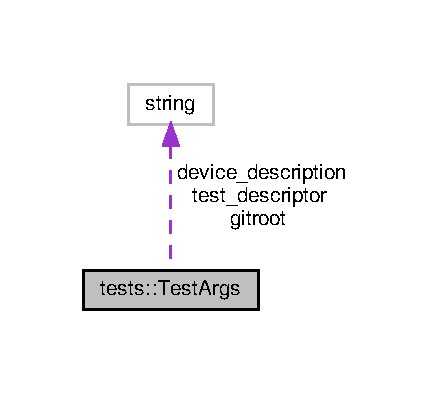
\includegraphics[width=207pt]{structtests_1_1TestArgs__coll__graph}
\end{center}
\end{figure}
\subsection*{Public Attributes}
\begin{DoxyCompactItemize}
\item 
std\+::string \hyperlink{structtests_1_1TestArgs_a3d843c12318312897e29428f6bc39c65}{device\+\_\+description}
\item 
std\+::string \hyperlink{structtests_1_1TestArgs_aac3629d45114721078dca6a6bb27b986}{test\+\_\+descriptor}
\item 
std\+::string \hyperlink{structtests_1_1TestArgs_a5fe492b8f262715e29547a81a4868d9f}{gitroot}
\item 
bool \hyperlink{structtests_1_1TestArgs_aae923f89bbd6b71b218a51fe6544481f}{dump\+\_\+tensors}
\item 
std\+::vector$<$ std\+::string $>$ \hyperlink{structtests_1_1TestArgs_a25bae49c946a2e91a641c644a0250063}{plusargs}
\item 
std\+::vector$<$ std\+::string $>$ \hyperlink{structtests_1_1TestArgs_a34d74d3077ef82959691a957a796e529}{dump\+\_\+cores}
\item 
bool \hyperlink{structtests_1_1TestArgs_a956bba7e1958d1e307955f8e3a46c02e}{regression\+\_\+mode}
\item 
bool \hyperlink{structtests_1_1TestArgs_a4d7793259b5f5b7543fe5df590c3744c}{force\+\_\+seed}
\item 
int \hyperlink{structtests_1_1TestArgs_a8e5b31cbcced7042e4f1cee4b4690a78}{seed}
\end{DoxyCompactItemize}


\subsection{Member Data Documentation}
\mbox{\Hypertarget{structtests_1_1TestArgs_a3d843c12318312897e29428f6bc39c65}\label{structtests_1_1TestArgs_a3d843c12318312897e29428f6bc39c65}} 
\index{tests\+::\+Test\+Args@{tests\+::\+Test\+Args}!device\+\_\+description@{device\+\_\+description}}
\index{device\+\_\+description@{device\+\_\+description}!tests\+::\+Test\+Args@{tests\+::\+Test\+Args}}
\subsubsection{\texorpdfstring{device\+\_\+description}{device\_description}}
{\footnotesize\ttfamily std\+::string tests\+::\+Test\+Args\+::device\+\_\+description}

\mbox{\Hypertarget{structtests_1_1TestArgs_a34d74d3077ef82959691a957a796e529}\label{structtests_1_1TestArgs_a34d74d3077ef82959691a957a796e529}} 
\index{tests\+::\+Test\+Args@{tests\+::\+Test\+Args}!dump\+\_\+cores@{dump\+\_\+cores}}
\index{dump\+\_\+cores@{dump\+\_\+cores}!tests\+::\+Test\+Args@{tests\+::\+Test\+Args}}
\subsubsection{\texorpdfstring{dump\+\_\+cores}{dump\_cores}}
{\footnotesize\ttfamily std\+::vector$<$std\+::string$>$ tests\+::\+Test\+Args\+::dump\+\_\+cores}

\mbox{\Hypertarget{structtests_1_1TestArgs_aae923f89bbd6b71b218a51fe6544481f}\label{structtests_1_1TestArgs_aae923f89bbd6b71b218a51fe6544481f}} 
\index{tests\+::\+Test\+Args@{tests\+::\+Test\+Args}!dump\+\_\+tensors@{dump\+\_\+tensors}}
\index{dump\+\_\+tensors@{dump\+\_\+tensors}!tests\+::\+Test\+Args@{tests\+::\+Test\+Args}}
\subsubsection{\texorpdfstring{dump\+\_\+tensors}{dump\_tensors}}
{\footnotesize\ttfamily bool tests\+::\+Test\+Args\+::dump\+\_\+tensors}

\mbox{\Hypertarget{structtests_1_1TestArgs_a4d7793259b5f5b7543fe5df590c3744c}\label{structtests_1_1TestArgs_a4d7793259b5f5b7543fe5df590c3744c}} 
\index{tests\+::\+Test\+Args@{tests\+::\+Test\+Args}!force\+\_\+seed@{force\+\_\+seed}}
\index{force\+\_\+seed@{force\+\_\+seed}!tests\+::\+Test\+Args@{tests\+::\+Test\+Args}}
\subsubsection{\texorpdfstring{force\+\_\+seed}{force\_seed}}
{\footnotesize\ttfamily bool tests\+::\+Test\+Args\+::force\+\_\+seed}

\mbox{\Hypertarget{structtests_1_1TestArgs_a5fe492b8f262715e29547a81a4868d9f}\label{structtests_1_1TestArgs_a5fe492b8f262715e29547a81a4868d9f}} 
\index{tests\+::\+Test\+Args@{tests\+::\+Test\+Args}!gitroot@{gitroot}}
\index{gitroot@{gitroot}!tests\+::\+Test\+Args@{tests\+::\+Test\+Args}}
\subsubsection{\texorpdfstring{gitroot}{gitroot}}
{\footnotesize\ttfamily std\+::string tests\+::\+Test\+Args\+::gitroot}

\mbox{\Hypertarget{structtests_1_1TestArgs_a25bae49c946a2e91a641c644a0250063}\label{structtests_1_1TestArgs_a25bae49c946a2e91a641c644a0250063}} 
\index{tests\+::\+Test\+Args@{tests\+::\+Test\+Args}!plusargs@{plusargs}}
\index{plusargs@{plusargs}!tests\+::\+Test\+Args@{tests\+::\+Test\+Args}}
\subsubsection{\texorpdfstring{plusargs}{plusargs}}
{\footnotesize\ttfamily std\+::vector$<$std\+::string$>$ tests\+::\+Test\+Args\+::plusargs}

\mbox{\Hypertarget{structtests_1_1TestArgs_a956bba7e1958d1e307955f8e3a46c02e}\label{structtests_1_1TestArgs_a956bba7e1958d1e307955f8e3a46c02e}} 
\index{tests\+::\+Test\+Args@{tests\+::\+Test\+Args}!regression\+\_\+mode@{regression\+\_\+mode}}
\index{regression\+\_\+mode@{regression\+\_\+mode}!tests\+::\+Test\+Args@{tests\+::\+Test\+Args}}
\subsubsection{\texorpdfstring{regression\+\_\+mode}{regression\_mode}}
{\footnotesize\ttfamily bool tests\+::\+Test\+Args\+::regression\+\_\+mode}

\mbox{\Hypertarget{structtests_1_1TestArgs_a8e5b31cbcced7042e4f1cee4b4690a78}\label{structtests_1_1TestArgs_a8e5b31cbcced7042e4f1cee4b4690a78}} 
\index{tests\+::\+Test\+Args@{tests\+::\+Test\+Args}!seed@{seed}}
\index{seed@{seed}!tests\+::\+Test\+Args@{tests\+::\+Test\+Args}}
\subsubsection{\texorpdfstring{seed}{seed}}
{\footnotesize\ttfamily int tests\+::\+Test\+Args\+::seed}

\mbox{\Hypertarget{structtests_1_1TestArgs_aac3629d45114721078dca6a6bb27b986}\label{structtests_1_1TestArgs_aac3629d45114721078dca6a6bb27b986}} 
\index{tests\+::\+Test\+Args@{tests\+::\+Test\+Args}!test\+\_\+descriptor@{test\+\_\+descriptor}}
\index{test\+\_\+descriptor@{test\+\_\+descriptor}!tests\+::\+Test\+Args@{tests\+::\+Test\+Args}}
\subsubsection{\texorpdfstring{test\+\_\+descriptor}{test\_descriptor}}
{\footnotesize\ttfamily std\+::string tests\+::\+Test\+Args\+::test\+\_\+descriptor}



The documentation for this struct was generated from the following file\+:\begin{DoxyCompactItemize}
\item 
tests/\hyperlink{test__args_8h}{test\+\_\+args.\+h}\end{DoxyCompactItemize}

\hypertarget{structtests_1_1TestConfig}{}\section{tests\+:\+:Test\+Config Struct Reference}
\label{structtests_1_1TestConfig}\index{tests\+::\+Test\+Config@{tests\+::\+Test\+Config}}


\hyperlink{structtests_1_1TestConfig}{Test\+Config} -\/ Config Structure.  




{\ttfamily \#include $<$test\+\_\+config.\+h$>$}



Collaboration diagram for tests\+:\+:Test\+Config\+:\nopagebreak
\begin{figure}[H]
\begin{center}
\leavevmode
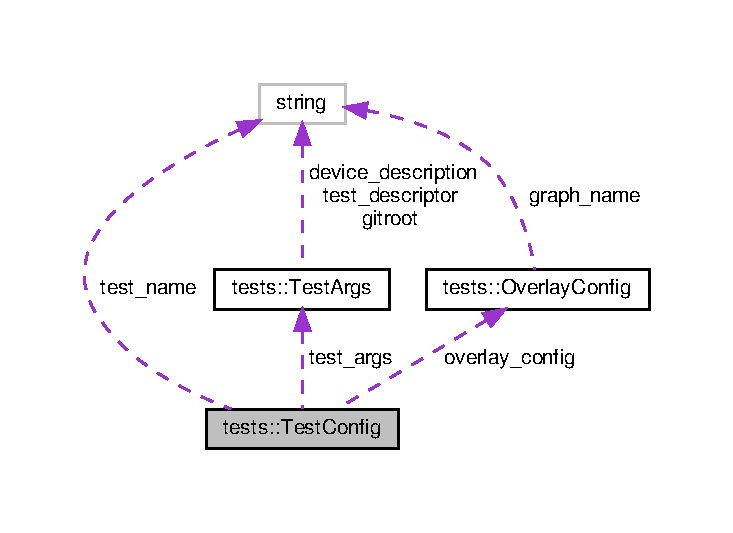
\includegraphics[width=350pt]{structtests_1_1TestConfig__coll__graph}
\end{center}
\end{figure}
\subsection*{Public Member Functions}
\begin{DoxyCompactItemize}
\item 
\hyperlink{structtests_1_1TestConfig_a32eac564ba880bb65d318e8f78de756b}{Test\+Config} (\hyperlink{structtests_1_1TestArgs}{Test\+Args} \hyperlink{structtests_1_1TestConfig_aa030c4b4c3fb91e5d6ac2524d408e727}{test\+\_\+args}, string \hyperlink{structtests_1_1TestConfig_aee3a781ac75f698787b6fcd81ca060bb}{test\+\_\+name}, bool \hyperlink{structtests_1_1TestConfig_ad3c14921521c690e03ab5664a69d9efc}{hlkc\+\_\+test}=false)
\item 
\hyperlink{structtests_1_1TestConfig_a169c374c99e645ce36d61113397220a0}{Test\+Config} (\hyperlink{structtests_1_1TestArgs}{Test\+Args} \hyperlink{structtests_1_1TestConfig_aa030c4b4c3fb91e5d6ac2524d408e727}{test\+\_\+args}, string \hyperlink{structtests_1_1TestConfig_aee3a781ac75f698787b6fcd81ca060bb}{test\+\_\+name}, Y\+A\+M\+L\+::\+Node test\+\_\+descriptor, bool \hyperlink{structtests_1_1TestConfig_ad3c14921521c690e03ab5664a69d9efc}{hlkc\+\_\+test}=false)
\end{DoxyCompactItemize}
\subsection*{Public Attributes}
\begin{DoxyCompactItemize}
\item 
\hyperlink{structtests_1_1TestArgs}{Test\+Args} \hyperlink{structtests_1_1TestConfig_aa030c4b4c3fb91e5d6ac2524d408e727}{test\+\_\+args}
\begin{DoxyCompactList}\small\item\em Global args from command line. \end{DoxyCompactList}\item 
string \hyperlink{structtests_1_1TestConfig_aee3a781ac75f698787b6fcd81ca060bb}{test\+\_\+name}
\item 
bool \hyperlink{structtests_1_1TestConfig_ad3c14921521c690e03ab5664a69d9efc}{hlkc\+\_\+test} = false
\item 
int \hyperlink{structtests_1_1TestConfig_a948808f31f8064964a14f33bd2e01068}{seed} = 0
\begin{DoxyCompactList}\small\item\em Seed used for stimulus and expected generation. \end{DoxyCompactList}\item 
map$<$ \hyperlink{structllk_1_1xy__pair}{llk\+::xy\+\_\+pair}, \hyperlink{structtests_1_1SingleCoreTestConfig}{Single\+Core\+Test\+Config} $>$ \hyperlink{structtests_1_1TestConfig_ae5193ec96cb529d0e40360c46e4b6b42}{core\+\_\+configs}
\begin{DoxyCompactList}\small\item\em Configs that are specified per core. contains kernel names and the related params. \end{DoxyCompactList}\item 
\hyperlink{structtests_1_1OverlayConfig}{Overlay\+Config} \hyperlink{structtests_1_1TestConfig_a985dffa5724992426ad6e6dc8e7fe39b}{overlay\+\_\+config}
\begin{DoxyCompactList}\small\item\em Overlay Configuration that specifies the flags for programming the overlay generation script. \end{DoxyCompactList}\item 
map$<$ string, \hyperlink{structtests_1_1TensorConfig}{Tensor\+Config} $>$ \hyperlink{structtests_1_1TestConfig_a0987a4cdba40e31d224181c17e5c042a}{tensor\+\_\+configs}
\begin{DoxyCompactList}\small\item\em Tensor Configuration which specifies the dimensions/data format/stimulus for the tensor. \end{DoxyCompactList}\item 
map$<$ string, string $>$ \hyperlink{structtests_1_1TestConfig_ac2374c533a372b8f7183de6215fe9791}{extra\+\_\+config}
\begin{DoxyCompactList}\small\item\em Extra Configs which test writer can add to and use in there test. \end{DoxyCompactList}\end{DoxyCompactItemize}


\subsection{Detailed Description}
\hyperlink{structtests_1_1TestConfig}{Test\+Config} -\/ Config Structure. 

\subsection{Constructor \& Destructor Documentation}
\mbox{\Hypertarget{structtests_1_1TestConfig_a32eac564ba880bb65d318e8f78de756b}\label{structtests_1_1TestConfig_a32eac564ba880bb65d318e8f78de756b}} 
\index{tests\+::\+Test\+Config@{tests\+::\+Test\+Config}!Test\+Config@{Test\+Config}}
\index{Test\+Config@{Test\+Config}!tests\+::\+Test\+Config@{tests\+::\+Test\+Config}}
\subsubsection{\texorpdfstring{Test\+Config()}{TestConfig()}\hspace{0.1cm}{\footnotesize\ttfamily [1/2]}}
{\footnotesize\ttfamily tests\+::\+Test\+Config\+::\+Test\+Config (\begin{DoxyParamCaption}\item[{\hyperlink{structtests_1_1TestArgs}{Test\+Args}}]{test\+\_\+args,  }\item[{string}]{test\+\_\+name,  }\item[{bool}]{hlkc\+\_\+test = {\ttfamily false} }\end{DoxyParamCaption})}

\mbox{\Hypertarget{structtests_1_1TestConfig_a169c374c99e645ce36d61113397220a0}\label{structtests_1_1TestConfig_a169c374c99e645ce36d61113397220a0}} 
\index{tests\+::\+Test\+Config@{tests\+::\+Test\+Config}!Test\+Config@{Test\+Config}}
\index{Test\+Config@{Test\+Config}!tests\+::\+Test\+Config@{tests\+::\+Test\+Config}}
\subsubsection{\texorpdfstring{Test\+Config()}{TestConfig()}\hspace{0.1cm}{\footnotesize\ttfamily [2/2]}}
{\footnotesize\ttfamily tests\+::\+Test\+Config\+::\+Test\+Config (\begin{DoxyParamCaption}\item[{\hyperlink{structtests_1_1TestArgs}{Test\+Args}}]{test\+\_\+args,  }\item[{string}]{test\+\_\+name,  }\item[{Y\+A\+M\+L\+::\+Node}]{test\+\_\+descriptor,  }\item[{bool}]{hlkc\+\_\+test = {\ttfamily false} }\end{DoxyParamCaption})}



\subsection{Member Data Documentation}
\mbox{\Hypertarget{structtests_1_1TestConfig_ae5193ec96cb529d0e40360c46e4b6b42}\label{structtests_1_1TestConfig_ae5193ec96cb529d0e40360c46e4b6b42}} 
\index{tests\+::\+Test\+Config@{tests\+::\+Test\+Config}!core\+\_\+configs@{core\+\_\+configs}}
\index{core\+\_\+configs@{core\+\_\+configs}!tests\+::\+Test\+Config@{tests\+::\+Test\+Config}}
\subsubsection{\texorpdfstring{core\+\_\+configs}{core\_configs}}
{\footnotesize\ttfamily map$<$\hyperlink{structllk_1_1xy__pair}{llk\+::xy\+\_\+pair}, \hyperlink{structtests_1_1SingleCoreTestConfig}{Single\+Core\+Test\+Config}$>$ tests\+::\+Test\+Config\+::core\+\_\+configs}



Configs that are specified per core. contains kernel names and the related params. 

Helper functions are available to read in the kernel names from yaml descriptor, kernel\+\_\+parameters have helper functions which can set it specifically \mbox{\Hypertarget{structtests_1_1TestConfig_ac2374c533a372b8f7183de6215fe9791}\label{structtests_1_1TestConfig_ac2374c533a372b8f7183de6215fe9791}} 
\index{tests\+::\+Test\+Config@{tests\+::\+Test\+Config}!extra\+\_\+config@{extra\+\_\+config}}
\index{extra\+\_\+config@{extra\+\_\+config}!tests\+::\+Test\+Config@{tests\+::\+Test\+Config}}
\subsubsection{\texorpdfstring{extra\+\_\+config}{extra\_config}}
{\footnotesize\ttfamily map$<$string, string$>$ tests\+::\+Test\+Config\+::extra\+\_\+config}



Extra Configs which test writer can add to and use in there test. 

\mbox{\Hypertarget{structtests_1_1TestConfig_ad3c14921521c690e03ab5664a69d9efc}\label{structtests_1_1TestConfig_ad3c14921521c690e03ab5664a69d9efc}} 
\index{tests\+::\+Test\+Config@{tests\+::\+Test\+Config}!hlkc\+\_\+test@{hlkc\+\_\+test}}
\index{hlkc\+\_\+test@{hlkc\+\_\+test}!tests\+::\+Test\+Config@{tests\+::\+Test\+Config}}
\subsubsection{\texorpdfstring{hlkc\+\_\+test}{hlkc\_test}}
{\footnotesize\ttfamily bool tests\+::\+Test\+Config\+::hlkc\+\_\+test = false}

\mbox{\Hypertarget{structtests_1_1TestConfig_a985dffa5724992426ad6e6dc8e7fe39b}\label{structtests_1_1TestConfig_a985dffa5724992426ad6e6dc8e7fe39b}} 
\index{tests\+::\+Test\+Config@{tests\+::\+Test\+Config}!overlay\+\_\+config@{overlay\+\_\+config}}
\index{overlay\+\_\+config@{overlay\+\_\+config}!tests\+::\+Test\+Config@{tests\+::\+Test\+Config}}
\subsubsection{\texorpdfstring{overlay\+\_\+config}{overlay\_config}}
{\footnotesize\ttfamily \hyperlink{structtests_1_1OverlayConfig}{Overlay\+Config} tests\+::\+Test\+Config\+::overlay\+\_\+config}



Overlay Configuration that specifies the flags for programming the overlay generation script. 

Helper functions are available to read in the config from yaml descriptor, and to automatically get updated if the tensor config changes \mbox{\Hypertarget{structtests_1_1TestConfig_a948808f31f8064964a14f33bd2e01068}\label{structtests_1_1TestConfig_a948808f31f8064964a14f33bd2e01068}} 
\index{tests\+::\+Test\+Config@{tests\+::\+Test\+Config}!seed@{seed}}
\index{seed@{seed}!tests\+::\+Test\+Config@{tests\+::\+Test\+Config}}
\subsubsection{\texorpdfstring{seed}{seed}}
{\footnotesize\ttfamily int tests\+::\+Test\+Config\+::seed = 0}



Seed used for stimulus and expected generation. 

\mbox{\Hypertarget{structtests_1_1TestConfig_a0987a4cdba40e31d224181c17e5c042a}\label{structtests_1_1TestConfig_a0987a4cdba40e31d224181c17e5c042a}} 
\index{tests\+::\+Test\+Config@{tests\+::\+Test\+Config}!tensor\+\_\+configs@{tensor\+\_\+configs}}
\index{tensor\+\_\+configs@{tensor\+\_\+configs}!tests\+::\+Test\+Config@{tests\+::\+Test\+Config}}
\subsubsection{\texorpdfstring{tensor\+\_\+configs}{tensor\_configs}}
{\footnotesize\ttfamily map$<$string, \hyperlink{structtests_1_1TensorConfig}{Tensor\+Config}$>$ tests\+::\+Test\+Config\+::tensor\+\_\+configs}



Tensor Configuration which specifies the dimensions/data format/stimulus for the tensor. 

Helper functions are available to read in the config from yaml descriptor \mbox{\Hypertarget{structtests_1_1TestConfig_aa030c4b4c3fb91e5d6ac2524d408e727}\label{structtests_1_1TestConfig_aa030c4b4c3fb91e5d6ac2524d408e727}} 
\index{tests\+::\+Test\+Config@{tests\+::\+Test\+Config}!test\+\_\+args@{test\+\_\+args}}
\index{test\+\_\+args@{test\+\_\+args}!tests\+::\+Test\+Config@{tests\+::\+Test\+Config}}
\subsubsection{\texorpdfstring{test\+\_\+args}{test\_args}}
{\footnotesize\ttfamily \hyperlink{structtests_1_1TestArgs}{Test\+Args} tests\+::\+Test\+Config\+::test\+\_\+args}



Global args from command line. 

\mbox{\Hypertarget{structtests_1_1TestConfig_aee3a781ac75f698787b6fcd81ca060bb}\label{structtests_1_1TestConfig_aee3a781ac75f698787b6fcd81ca060bb}} 
\index{tests\+::\+Test\+Config@{tests\+::\+Test\+Config}!test\+\_\+name@{test\+\_\+name}}
\index{test\+\_\+name@{test\+\_\+name}!tests\+::\+Test\+Config@{tests\+::\+Test\+Config}}
\subsubsection{\texorpdfstring{test\+\_\+name}{test\_name}}
{\footnotesize\ttfamily string tests\+::\+Test\+Config\+::test\+\_\+name}



The documentation for this struct was generated from the following file\+:\begin{DoxyCompactItemize}
\item 
tests/\hyperlink{test__config_8h}{test\+\_\+config.\+h}\end{DoxyCompactItemize}

\hypertarget{structllk_1_1xy__pair}{}\section{llk\+:\+:xy\+\_\+pair Struct Reference}
\label{structllk_1_1xy__pair}\index{llk\+::xy\+\_\+pair@{llk\+::xy\+\_\+pair}}


{\ttfamily \#include $<$llk\+\_\+xy\+\_\+pair.\+h$>$}

\subsection*{Public Member Functions}
\begin{DoxyCompactItemize}
\item 
\hyperlink{structllk_1_1xy__pair_ae83534da806de13692d9a1f513a61968}{xy\+\_\+pair} ()
\item 
constexpr \hyperlink{structllk_1_1xy__pair_aa8dc8fdc3fd5663ef038996ef30aa5b8}{xy\+\_\+pair} (std\+::size\+\_\+t \hyperlink{structllk_1_1xy__pair_a0529eda73df053ddcc7662187ca57e23}{x}, std\+::size\+\_\+t \hyperlink{structllk_1_1xy__pair_a95998ff2c605752606fea129d2adb409}{y})
\item 
{\footnotesize template$<$typename Pair $>$ }\\\hyperlink{structllk_1_1xy__pair_ac5524e1982092fb9355deb5a5f440192}{xy\+\_\+pair} (const Pair \&p)
\item 
\hyperlink{structllk_1_1xy__pair_aec16ff0f0fbd56708059f48769c4af8c}{xy\+\_\+pair} (const Command\+Assembler\+::xy\+\_\+pair \&p)
\item 
{\footnotesize template$<$class Function $>$ }\\void \hyperlink{structllk_1_1xy__pair_aee809f43444011ef5a89878e6c32b9bb}{for\+\_\+each} (Function \&\&f) const
\item 
\hyperlink{structllk_1_1xy__pair}{xy\+\_\+pair} \hyperlink{structllk_1_1xy__pair_a43aa7e67327dbb79cd6d040ea77c0d04}{operator+} (const \hyperlink{structllk_1_1xy__pair}{xy\+\_\+pair} \&right)
\item 
std\+::string \hyperlink{structllk_1_1xy__pair_ad3c688d70663331110ac68bdce324c48}{str} () const
\item 
std\+::string \hyperlink{structllk_1_1xy__pair_a4fa9ce275bc72c1b98ffdf9e7b7e7797}{str} ()
\item 
\hyperlink{structllk_1_1xy__pair_afdde5bcb5672613be31f7cad5d798857}{operator Command\+Assembler\+::xy\+\_\+pair} () const
\end{DoxyCompactItemize}
\subsection*{Static Public Member Functions}
\begin{DoxyCompactItemize}
\item 
static \hyperlink{structllk_1_1xy__pair}{xy\+\_\+pair} \hyperlink{structllk_1_1xy__pair_ac9e9ac443b0172af1da1157ecdc8665a}{parse} (const std\+::string \&s)
\end{DoxyCompactItemize}
\subsection*{Public Attributes}
\begin{DoxyCompactItemize}
\item 
std\+::size\+\_\+t \hyperlink{structllk_1_1xy__pair_a0529eda73df053ddcc7662187ca57e23}{x}
\item 
std\+::size\+\_\+t \hyperlink{structllk_1_1xy__pair_a95998ff2c605752606fea129d2adb409}{y}
\item 
std\+::size\+\_\+t \hyperlink{structllk_1_1xy__pair_acec3f70be79e2e1ccbf2e40853a85101}{first}
\item 
std\+::size\+\_\+t \hyperlink{structllk_1_1xy__pair_ab150c1eaffd7963239c139d330851e67}{second}
\end{DoxyCompactItemize}


\subsection{Constructor \& Destructor Documentation}
\mbox{\Hypertarget{structllk_1_1xy__pair_ae83534da806de13692d9a1f513a61968}\label{structllk_1_1xy__pair_ae83534da806de13692d9a1f513a61968}} 
\index{llk\+::xy\+\_\+pair@{llk\+::xy\+\_\+pair}!xy\+\_\+pair@{xy\+\_\+pair}}
\index{xy\+\_\+pair@{xy\+\_\+pair}!llk\+::xy\+\_\+pair@{llk\+::xy\+\_\+pair}}
\subsubsection{\texorpdfstring{xy\+\_\+pair()}{xy\_pair()}\hspace{0.1cm}{\footnotesize\ttfamily [1/4]}}
{\footnotesize\ttfamily llk\+::xy\+\_\+pair\+::xy\+\_\+pair (\begin{DoxyParamCaption}{ }\end{DoxyParamCaption})\hspace{0.3cm}{\ttfamily [inline]}}

\mbox{\Hypertarget{structllk_1_1xy__pair_aa8dc8fdc3fd5663ef038996ef30aa5b8}\label{structllk_1_1xy__pair_aa8dc8fdc3fd5663ef038996ef30aa5b8}} 
\index{llk\+::xy\+\_\+pair@{llk\+::xy\+\_\+pair}!xy\+\_\+pair@{xy\+\_\+pair}}
\index{xy\+\_\+pair@{xy\+\_\+pair}!llk\+::xy\+\_\+pair@{llk\+::xy\+\_\+pair}}
\subsubsection{\texorpdfstring{xy\+\_\+pair()}{xy\_pair()}\hspace{0.1cm}{\footnotesize\ttfamily [2/4]}}
{\footnotesize\ttfamily constexpr llk\+::xy\+\_\+pair\+::xy\+\_\+pair (\begin{DoxyParamCaption}\item[{std\+::size\+\_\+t}]{x,  }\item[{std\+::size\+\_\+t}]{y }\end{DoxyParamCaption})\hspace{0.3cm}{\ttfamily [inline]}}

\mbox{\Hypertarget{structllk_1_1xy__pair_ac5524e1982092fb9355deb5a5f440192}\label{structllk_1_1xy__pair_ac5524e1982092fb9355deb5a5f440192}} 
\index{llk\+::xy\+\_\+pair@{llk\+::xy\+\_\+pair}!xy\+\_\+pair@{xy\+\_\+pair}}
\index{xy\+\_\+pair@{xy\+\_\+pair}!llk\+::xy\+\_\+pair@{llk\+::xy\+\_\+pair}}
\subsubsection{\texorpdfstring{xy\+\_\+pair()}{xy\_pair()}\hspace{0.1cm}{\footnotesize\ttfamily [3/4]}}
{\footnotesize\ttfamily template$<$typename Pair $>$ \\
llk\+::xy\+\_\+pair\+::xy\+\_\+pair (\begin{DoxyParamCaption}\item[{const Pair \&}]{p }\end{DoxyParamCaption})\hspace{0.3cm}{\ttfamily [inline]}, {\ttfamily [explicit]}}

\mbox{\Hypertarget{structllk_1_1xy__pair_aec16ff0f0fbd56708059f48769c4af8c}\label{structllk_1_1xy__pair_aec16ff0f0fbd56708059f48769c4af8c}} 
\index{llk\+::xy\+\_\+pair@{llk\+::xy\+\_\+pair}!xy\+\_\+pair@{xy\+\_\+pair}}
\index{xy\+\_\+pair@{xy\+\_\+pair}!llk\+::xy\+\_\+pair@{llk\+::xy\+\_\+pair}}
\subsubsection{\texorpdfstring{xy\+\_\+pair()}{xy\_pair()}\hspace{0.1cm}{\footnotesize\ttfamily [4/4]}}
{\footnotesize\ttfamily llk\+::xy\+\_\+pair\+::xy\+\_\+pair (\begin{DoxyParamCaption}\item[{const Command\+Assembler\+::xy\+\_\+pair \&}]{p }\end{DoxyParamCaption})\hspace{0.3cm}{\ttfamily [inline]}, {\ttfamily [explicit]}}



\subsection{Member Function Documentation}
\mbox{\Hypertarget{structllk_1_1xy__pair_aee809f43444011ef5a89878e6c32b9bb}\label{structllk_1_1xy__pair_aee809f43444011ef5a89878e6c32b9bb}} 
\index{llk\+::xy\+\_\+pair@{llk\+::xy\+\_\+pair}!for\+\_\+each@{for\+\_\+each}}
\index{for\+\_\+each@{for\+\_\+each}!llk\+::xy\+\_\+pair@{llk\+::xy\+\_\+pair}}
\subsubsection{\texorpdfstring{for\+\_\+each()}{for\_each()}}
{\footnotesize\ttfamily template$<$class Function $>$ \\
void llk\+::xy\+\_\+pair\+::for\+\_\+each (\begin{DoxyParamCaption}\item[{Function \&\&}]{f }\end{DoxyParamCaption}) const}

\mbox{\Hypertarget{structllk_1_1xy__pair_afdde5bcb5672613be31f7cad5d798857}\label{structllk_1_1xy__pair_afdde5bcb5672613be31f7cad5d798857}} 
\index{llk\+::xy\+\_\+pair@{llk\+::xy\+\_\+pair}!operator Command\+Assembler\+::xy\+\_\+pair@{operator Command\+Assembler\+::xy\+\_\+pair}}
\index{operator Command\+Assembler\+::xy\+\_\+pair@{operator Command\+Assembler\+::xy\+\_\+pair}!llk\+::xy\+\_\+pair@{llk\+::xy\+\_\+pair}}
\subsubsection{\texorpdfstring{operator Command\+Assembler\+::xy\+\_\+pair()}{operator CommandAssembler::xy\_pair()}}
{\footnotesize\ttfamily llk\+::xy\+\_\+pair\+::operator Command\+Assembler\+::xy\+\_\+pair (\begin{DoxyParamCaption}{ }\end{DoxyParamCaption}) const\hspace{0.3cm}{\ttfamily [inline]}}

\mbox{\Hypertarget{structllk_1_1xy__pair_a43aa7e67327dbb79cd6d040ea77c0d04}\label{structllk_1_1xy__pair_a43aa7e67327dbb79cd6d040ea77c0d04}} 
\index{llk\+::xy\+\_\+pair@{llk\+::xy\+\_\+pair}!operator+@{operator+}}
\index{operator+@{operator+}!llk\+::xy\+\_\+pair@{llk\+::xy\+\_\+pair}}
\subsubsection{\texorpdfstring{operator+()}{operator+()}}
{\footnotesize\ttfamily \hyperlink{structllk_1_1xy__pair}{xy\+\_\+pair} llk\+::xy\+\_\+pair\+::operator+ (\begin{DoxyParamCaption}\item[{const \hyperlink{structllk_1_1xy__pair}{xy\+\_\+pair} \&}]{right }\end{DoxyParamCaption})\hspace{0.3cm}{\ttfamily [inline]}}

\mbox{\Hypertarget{structllk_1_1xy__pair_ac9e9ac443b0172af1da1157ecdc8665a}\label{structllk_1_1xy__pair_ac9e9ac443b0172af1da1157ecdc8665a}} 
\index{llk\+::xy\+\_\+pair@{llk\+::xy\+\_\+pair}!parse@{parse}}
\index{parse@{parse}!llk\+::xy\+\_\+pair@{llk\+::xy\+\_\+pair}}
\subsubsection{\texorpdfstring{parse()}{parse()}}
{\footnotesize\ttfamily \hyperlink{structllk_1_1xy__pair}{xy\+\_\+pair} xy\+\_\+pair\+::parse (\begin{DoxyParamCaption}\item[{const std\+::string \&}]{s }\end{DoxyParamCaption})\hspace{0.3cm}{\ttfamily [static]}}

\mbox{\Hypertarget{structllk_1_1xy__pair_ad3c688d70663331110ac68bdce324c48}\label{structllk_1_1xy__pair_ad3c688d70663331110ac68bdce324c48}} 
\index{llk\+::xy\+\_\+pair@{llk\+::xy\+\_\+pair}!str@{str}}
\index{str@{str}!llk\+::xy\+\_\+pair@{llk\+::xy\+\_\+pair}}
\subsubsection{\texorpdfstring{str()}{str()}\hspace{0.1cm}{\footnotesize\ttfamily [1/2]}}
{\footnotesize\ttfamily std\+::string llk\+::xy\+\_\+pair\+::str (\begin{DoxyParamCaption}{ }\end{DoxyParamCaption}) const\hspace{0.3cm}{\ttfamily [inline]}}

\mbox{\Hypertarget{structllk_1_1xy__pair_a4fa9ce275bc72c1b98ffdf9e7b7e7797}\label{structllk_1_1xy__pair_a4fa9ce275bc72c1b98ffdf9e7b7e7797}} 
\index{llk\+::xy\+\_\+pair@{llk\+::xy\+\_\+pair}!str@{str}}
\index{str@{str}!llk\+::xy\+\_\+pair@{llk\+::xy\+\_\+pair}}
\subsubsection{\texorpdfstring{str()}{str()}\hspace{0.1cm}{\footnotesize\ttfamily [2/2]}}
{\footnotesize\ttfamily std\+::string llk\+::xy\+\_\+pair\+::str (\begin{DoxyParamCaption}{ }\end{DoxyParamCaption})\hspace{0.3cm}{\ttfamily [inline]}}



\subsection{Member Data Documentation}
\mbox{\Hypertarget{structllk_1_1xy__pair_acec3f70be79e2e1ccbf2e40853a85101}\label{structllk_1_1xy__pair_acec3f70be79e2e1ccbf2e40853a85101}} 
\index{llk\+::xy\+\_\+pair@{llk\+::xy\+\_\+pair}!first@{first}}
\index{first@{first}!llk\+::xy\+\_\+pair@{llk\+::xy\+\_\+pair}}
\subsubsection{\texorpdfstring{first}{first}}
{\footnotesize\ttfamily std\+::size\+\_\+t llk\+::xy\+\_\+pair\+::first}

\mbox{\Hypertarget{structllk_1_1xy__pair_ab150c1eaffd7963239c139d330851e67}\label{structllk_1_1xy__pair_ab150c1eaffd7963239c139d330851e67}} 
\index{llk\+::xy\+\_\+pair@{llk\+::xy\+\_\+pair}!second@{second}}
\index{second@{second}!llk\+::xy\+\_\+pair@{llk\+::xy\+\_\+pair}}
\subsubsection{\texorpdfstring{second}{second}}
{\footnotesize\ttfamily std\+::size\+\_\+t llk\+::xy\+\_\+pair\+::second}

\mbox{\Hypertarget{structllk_1_1xy__pair_a0529eda73df053ddcc7662187ca57e23}\label{structllk_1_1xy__pair_a0529eda73df053ddcc7662187ca57e23}} 
\index{llk\+::xy\+\_\+pair@{llk\+::xy\+\_\+pair}!x@{x}}
\index{x@{x}!llk\+::xy\+\_\+pair@{llk\+::xy\+\_\+pair}}
\subsubsection{\texorpdfstring{x}{x}}
{\footnotesize\ttfamily std\+::size\+\_\+t llk\+::xy\+\_\+pair\+::x}

\mbox{\Hypertarget{structllk_1_1xy__pair_a95998ff2c605752606fea129d2adb409}\label{structllk_1_1xy__pair_a95998ff2c605752606fea129d2adb409}} 
\index{llk\+::xy\+\_\+pair@{llk\+::xy\+\_\+pair}!y@{y}}
\index{y@{y}!llk\+::xy\+\_\+pair@{llk\+::xy\+\_\+pair}}
\subsubsection{\texorpdfstring{y}{y}}
{\footnotesize\ttfamily std\+::size\+\_\+t llk\+::xy\+\_\+pair\+::y}



The documentation for this struct was generated from the following files\+:\begin{DoxyCompactItemize}
\item 
inc/\hyperlink{llk__xy__pair_8h}{llk\+\_\+xy\+\_\+pair.\+h}\item 
src/\hyperlink{llk__xy__pair_8cpp}{llk\+\_\+xy\+\_\+pair.\+cpp}\end{DoxyCompactItemize}

\chapter{File Documentation}
\hypertarget{llk__addresses_8h}{}\section{inc/llk\+\_\+addresses.h File Reference}
\label{llk__addresses_8h}\index{inc/llk\+\_\+addresses.\+h@{inc/llk\+\_\+addresses.\+h}}
{\ttfamily \#include \char`\"{}l1\+\_\+address\+\_\+map.\+h\char`\"{}}\newline
Include dependency graph for llk\+\_\+addresses.\+h\+:\nopagebreak
\begin{figure}[H]
\begin{center}
\leavevmode
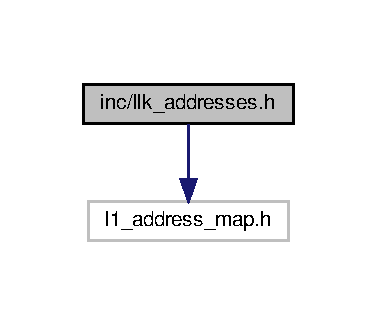
\includegraphics[width=181pt]{llk__addresses_8h__incl}
\end{center}
\end{figure}
This graph shows which files directly or indirectly include this file\+:\nopagebreak
\begin{figure}[H]
\begin{center}
\leavevmode
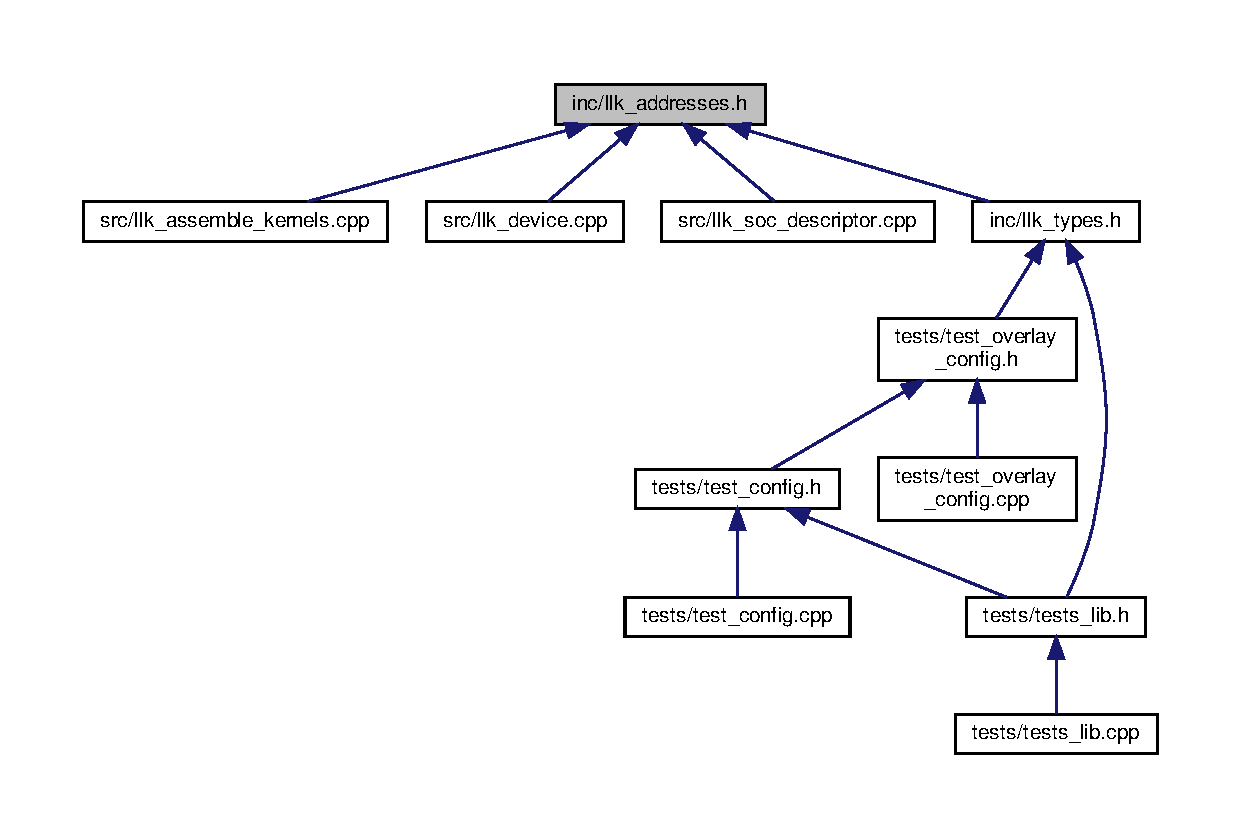
\includegraphics[width=350pt]{llk__addresses_8h__dep__incl}
\end{center}
\end{figure}
\subsection*{Classes}
\begin{DoxyCompactItemize}
\item 
struct \hyperlink{structllk_1_1test__address__map}{llk\+::test\+\_\+address\+\_\+map}
\end{DoxyCompactItemize}
\subsection*{Namespaces}
\begin{DoxyCompactItemize}
\item 
 \hyperlink{namespacellk}{llk}
\end{DoxyCompactItemize}

\hypertarget{llk__assemble__kernels_8h}{}\section{inc/llk\+\_\+assemble\+\_\+kernels.h File Reference}
\label{llk__assemble__kernels_8h}\index{inc/llk\+\_\+assemble\+\_\+kernels.\+h@{inc/llk\+\_\+assemble\+\_\+kernels.\+h}}
{\ttfamily \#include $<$string$>$}\newline
{\ttfamily \#include $<$unordered\+\_\+map$>$}\newline
{\ttfamily \#include $<$vector$>$}\newline
{\ttfamily \#include \char`\"{}llk\+\_\+memory.\+h\char`\"{}}\newline
{\ttfamily \#include \char`\"{}llk\+\_\+soc\+\_\+descriptor.\+h\char`\"{}}\newline
{\ttfamily \#include \char`\"{}llk\+\_\+xy\+\_\+pair.\+h\char`\"{}}\newline
Include dependency graph for llk\+\_\+assemble\+\_\+kernels.\+h\+:\nopagebreak
\begin{figure}[H]
\begin{center}
\leavevmode
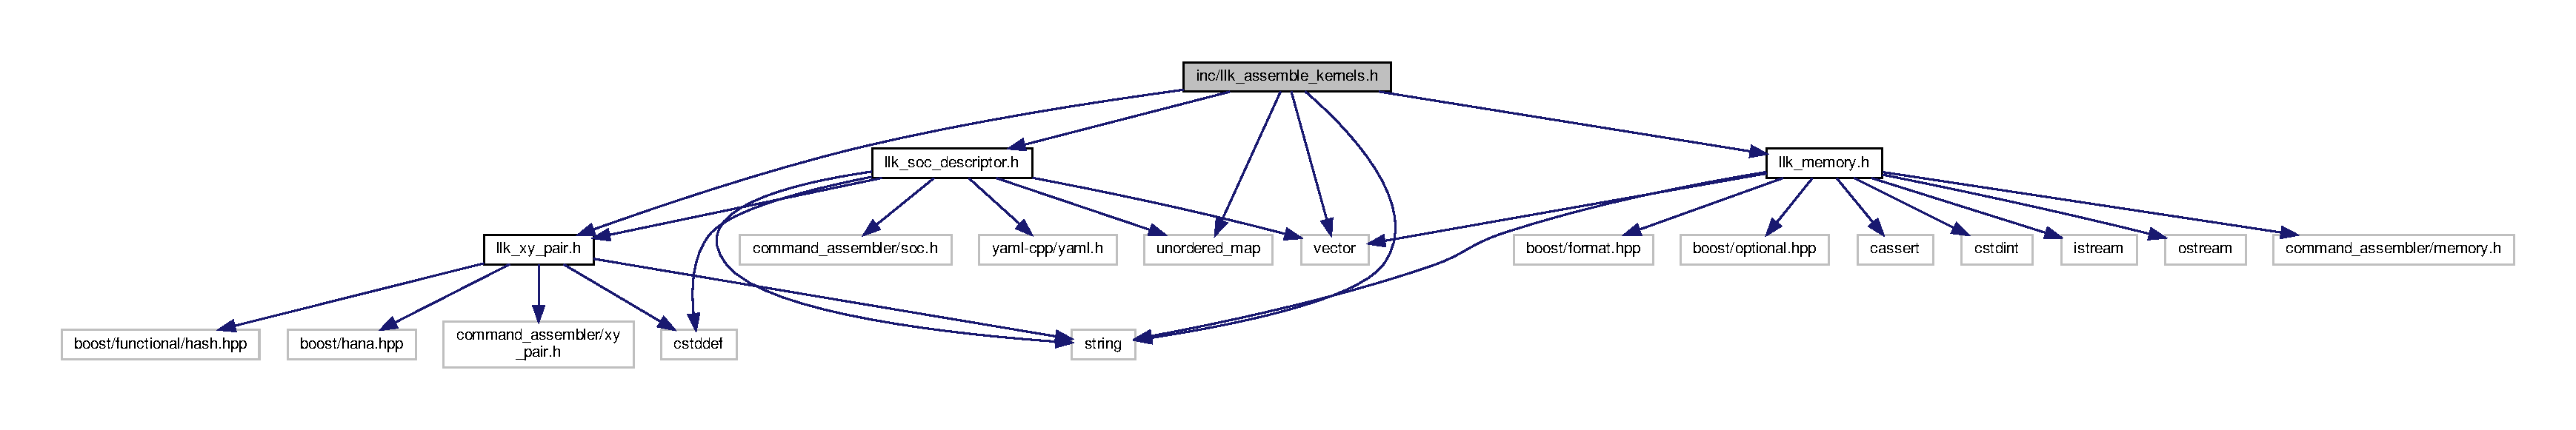
\includegraphics[width=350pt]{llk__assemble__kernels_8h__incl}
\end{center}
\end{figure}
This graph shows which files directly or indirectly include this file\+:\nopagebreak
\begin{figure}[H]
\begin{center}
\leavevmode
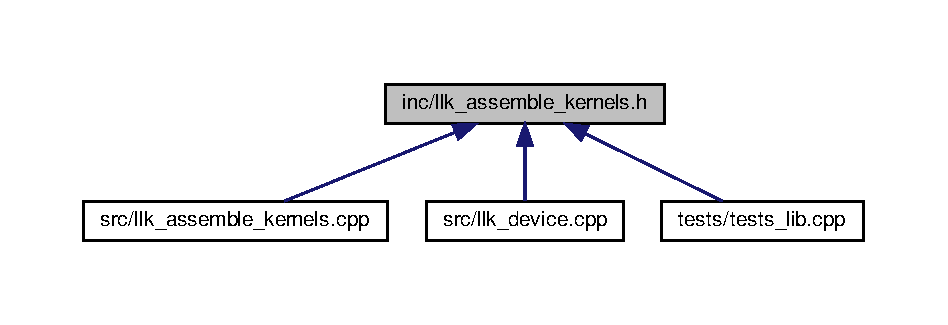
\includegraphics[width=350pt]{llk__assemble__kernels_8h__dep__incl}
\end{center}
\end{figure}
\subsection*{Namespaces}
\begin{DoxyCompactItemize}
\item 
 \hyperlink{namespacellk}{llk}
\item 
 \hyperlink{namespacellk_1_1assemble__kernels}{llk\+::assemble\+\_\+kernels}
\begin{DoxyCompactList}\small\item\em \hyperlink{namespacellk_1_1assemble__kernels}{assemble\+\_\+kernels} meant to assemble and build kernel memories \end{DoxyCompactList}\end{DoxyCompactItemize}
\subsection*{Functions}
\begin{DoxyCompactItemize}
\item 
bool \hyperlink{namespacellk_1_1assemble__kernels_a5216f630a6ff0cb75b43ebf8adf1a93e}{llk\+::assemble\+\_\+kernels\+::run\+\_\+command} (const std\+::string \&cmd)
\item 
void \hyperlink{namespacellk_1_1assemble__kernels_a188966c139ddbc16fe641bcb1fc73daa}{llk\+::assemble\+\_\+kernels\+::generate\+\_\+kernel\+\_\+param\+\_\+file} (const std\+::string \&kernel\+\_\+name, const std\+::string \&generate\+\_\+kernel\+\_\+param\+\_\+file, const std\+::string \&outdir, const std\+::map$<$ std\+::string, std\+::string $>$ \&kernel\+\_\+params=\{\})
\item 
\hyperlink{classllk_1_1memory}{llk\+::memory} \hyperlink{namespacellk_1_1assemble__kernels_a0c64d9c4bdd026cef18dbede1e95f601}{llk\+::assemble\+\_\+kernels\+::build\+\_\+kernel\+\_\+memories\+\_\+per\+\_\+trisc\+\_\+thread} (std\+::string output\+\_\+dir, std\+::string make\+\_\+src\+\_\+args, std\+::string make\+\_\+args, std\+::string test\+\_\+name, std\+::uint32\+\_\+t $\ast$trisc\+\_\+mailbox\+\_\+addresses, int thread\+\_\+id, bool hlkc\+\_\+kernels, std\+::string used\+\_\+kernels, std\+::string \&fwlog\+\_\+string)
\item 
void \hyperlink{namespacellk_1_1assemble__kernels_ac86be485d5e20c3e05809d2f00e63cfd}{llk\+::assemble\+\_\+kernels\+::compile\+\_\+kernels} (std\+::string output\+\_\+dir, std\+::string make\+\_\+src\+\_\+args, std\+::string make\+\_\+args, std\+::string test\+\_\+name, std\+::uint32\+\_\+t trisc\+\_\+mailbox\+\_\+addr, int thread\+\_\+id, bool hlkc\+\_\+kernels, std\+::string used\+\_\+kernels)
\item 
void \hyperlink{namespacellk_1_1assemble__kernels_a7aa5c5270196ee870fd874bc6c5b30aa}{llk\+::assemble\+\_\+kernels\+::build\+\_\+kernel\+\_\+memories} (\hyperlink{structllk_1_1SocDescriptor}{llk\+::\+Soc\+Descriptor} soc\+\_\+descriptor, std\+::string root, bool hlkc\+\_\+kernels, std\+::string test\+\_\+name, std\+::unordered\+\_\+map$<$ \hyperlink{structllk_1_1xy__pair}{llk\+::xy\+\_\+pair}, std\+::vector$<$ std\+::vector$<$ std\+::string $>$$>$$>$ \&kernels\+\_\+used, std\+::unordered\+\_\+map$<$ \hyperlink{structllk_1_1xy__pair}{llk\+::xy\+\_\+pair}, std\+::vector$<$ \hyperlink{classllk_1_1memory}{llk\+::memory} $>$$>$ \&ckernel\+\_\+memories, std\+::unordered\+\_\+map$<$ \hyperlink{structllk_1_1xy__pair}{llk\+::xy\+\_\+pair}, std\+::string $>$ \&fwlogs)
\end{DoxyCompactItemize}

\hypertarget{llk__device_8h}{}\section{inc/llk\+\_\+device.h File Reference}
\label{llk__device_8h}\index{inc/llk\+\_\+device.\+h@{inc/llk\+\_\+device.\+h}}
{\ttfamily \#include $<$map$>$}\newline
{\ttfamily \#include $<$string$>$}\newline
{\ttfamily \#include $<$unordered\+\_\+map$>$}\newline
{\ttfamily \#include $<$vector$>$}\newline
{\ttfamily \#include \char`\"{}llk\+\_\+soc\+\_\+descriptor.\+h\char`\"{}}\newline
{\ttfamily \#include \char`\"{}llk\+\_\+tensor.\+h\char`\"{}}\newline
{\ttfamily \#include \char`\"{}llk\+\_\+xy\+\_\+pair.\+h\char`\"{}}\newline
{\ttfamily \#include \char`\"{}device.\+h\char`\"{}}\newline
{\ttfamily \#include \char`\"{}sim\+\_\+interactive.\+h\char`\"{}}\newline
Include dependency graph for llk\+\_\+device.\+h\+:\nopagebreak
\begin{figure}[H]
\begin{center}
\leavevmode
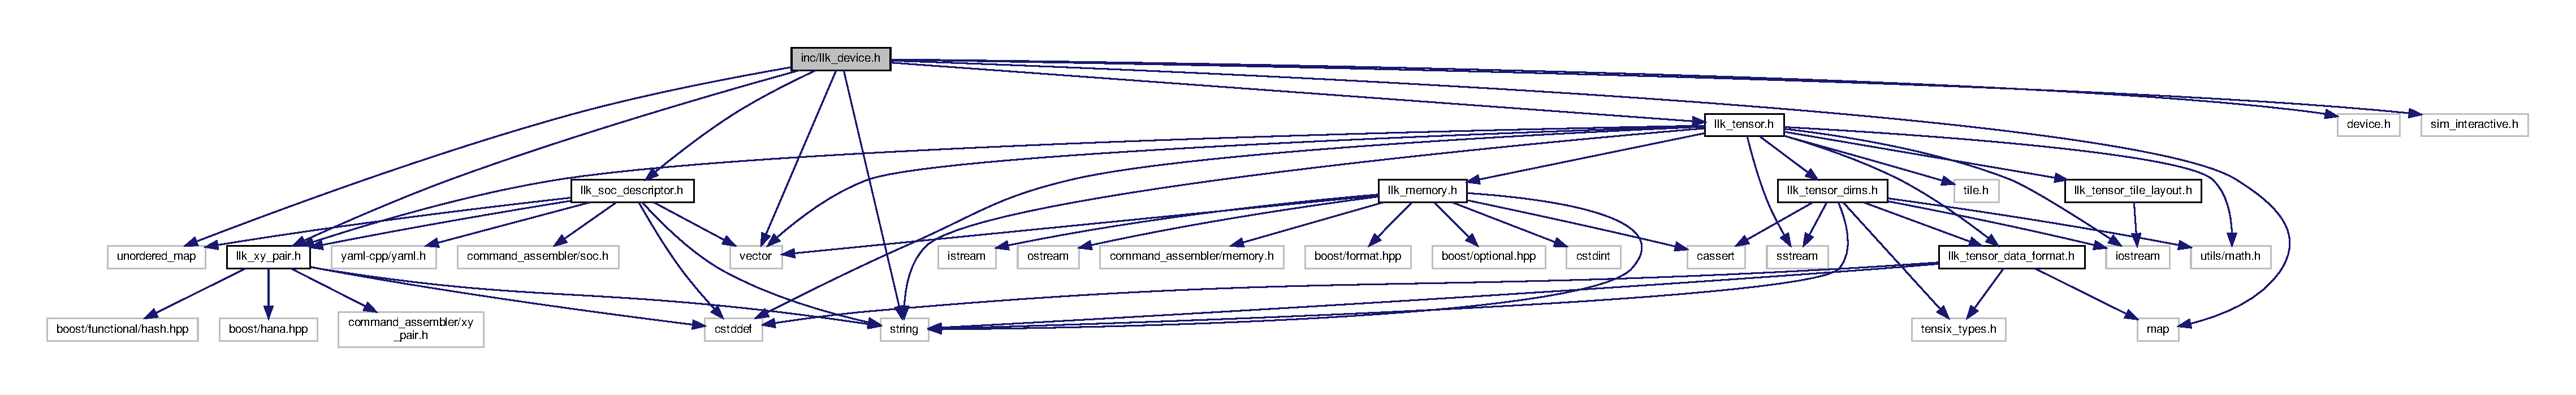
\includegraphics[width=350pt]{llk__device_8h__incl}
\end{center}
\end{figure}
This graph shows which files directly or indirectly include this file\+:\nopagebreak
\begin{figure}[H]
\begin{center}
\leavevmode
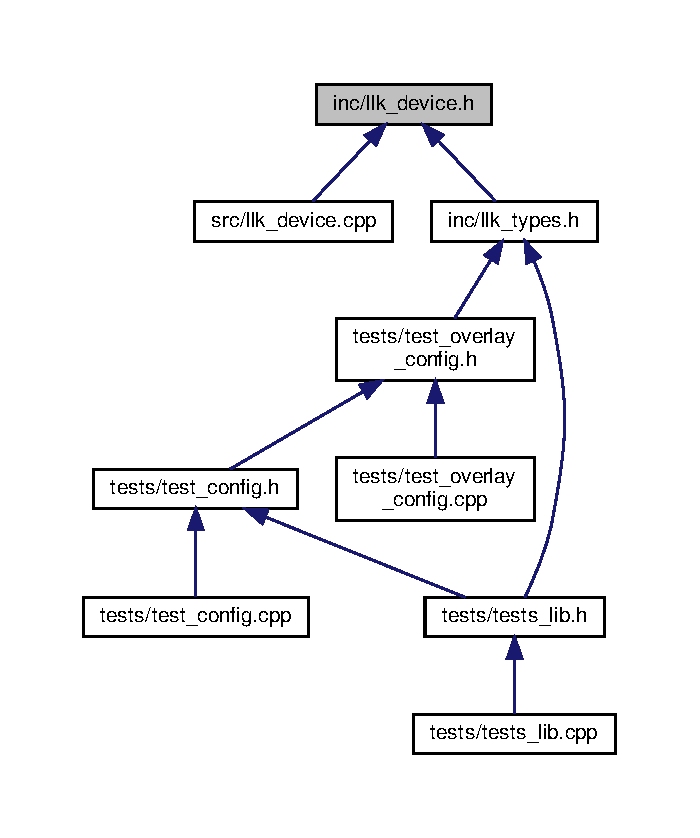
\includegraphics[width=336pt]{llk__device_8h__dep__incl}
\end{center}
\end{figure}
\subsection*{Classes}
\begin{DoxyCompactItemize}
\item 
class \hyperlink{classllk_1_1Device}{llk\+::\+Device}
\begin{DoxyCompactList}\small\item\em \hyperlink{classllk_1_1Device}{Device} A\+PI in a wrapper class. \end{DoxyCompactList}\end{DoxyCompactItemize}
\subsection*{Namespaces}
\begin{DoxyCompactItemize}
\item 
 \hyperlink{namespacellk}{llk}
\end{DoxyCompactItemize}

\hypertarget{llk__hexfile_8h}{}\section{inc/llk\+\_\+hexfile.h File Reference}
\label{llk__hexfile_8h}\index{inc/llk\+\_\+hexfile.\+h@{inc/llk\+\_\+hexfile.\+h}}
{\ttfamily \#include $<$boost/io/ios\+\_\+state.\+hpp$>$}\newline
{\ttfamily \#include $<$istream$>$}\newline
{\ttfamily \#include $<$ostream$>$}\newline
{\ttfamily \#include $<$vector$>$}\newline
{\ttfamily \#include \char`\"{}llk\+\_\+memory.\+h\char`\"{}}\newline
Include dependency graph for llk\+\_\+hexfile.\+h\+:\nopagebreak
\begin{figure}[H]
\begin{center}
\leavevmode
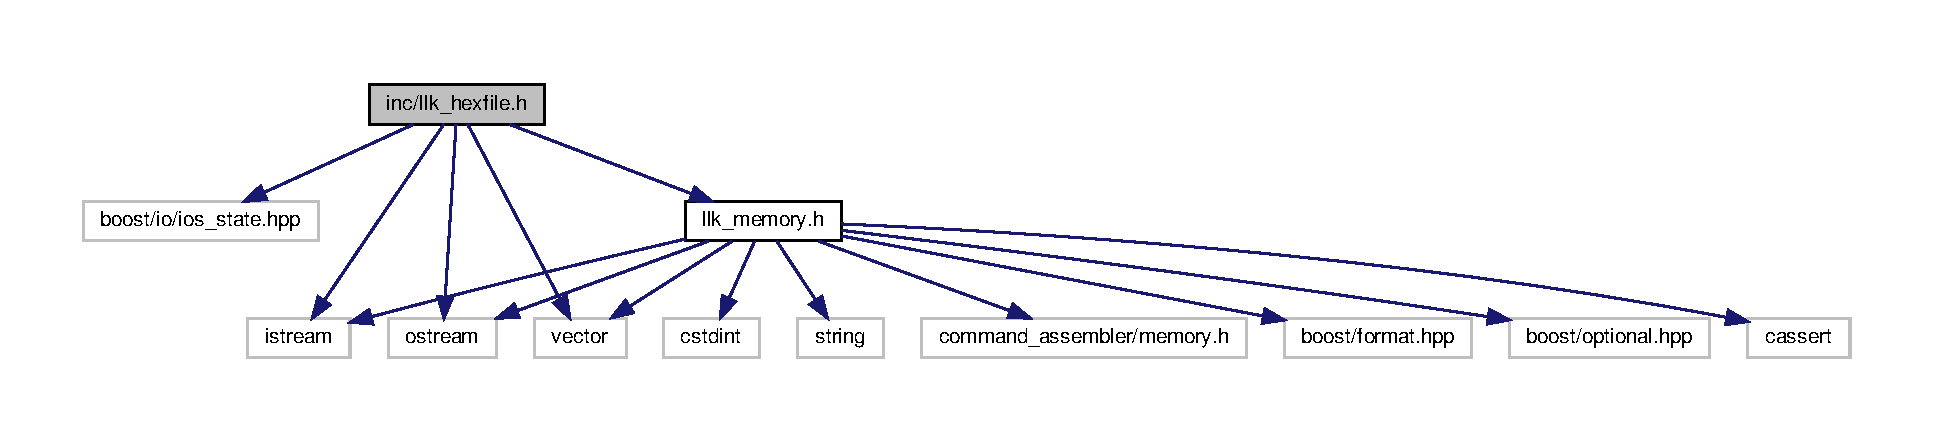
\includegraphics[width=350pt]{llk__hexfile_8h__incl}
\end{center}
\end{figure}
This graph shows which files directly or indirectly include this file\+:\nopagebreak
\begin{figure}[H]
\begin{center}
\leavevmode
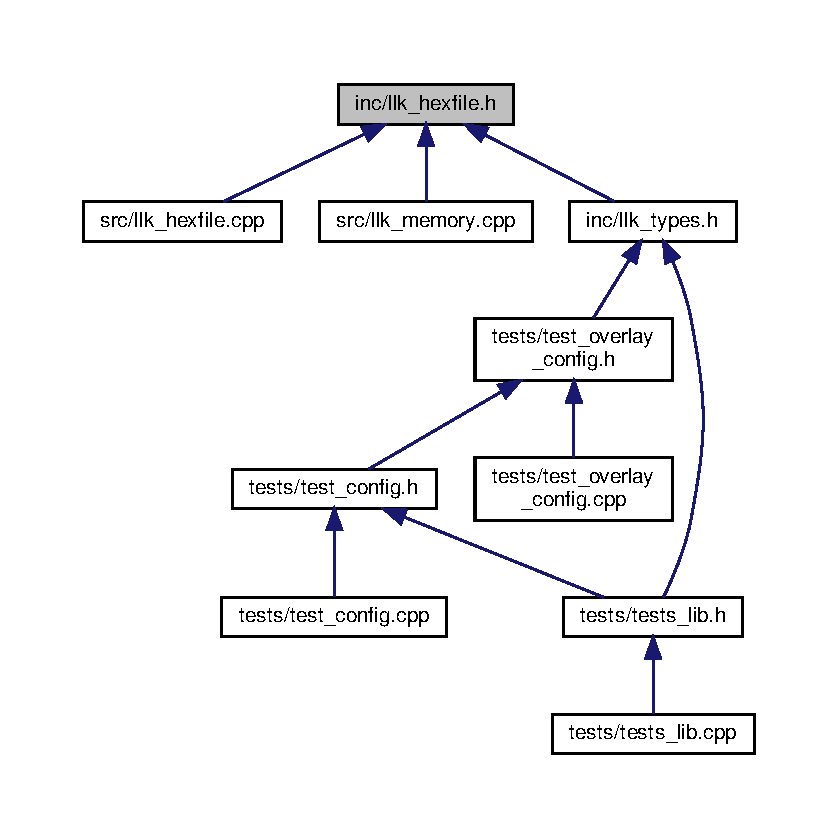
\includegraphics[width=350pt]{llk__hexfile_8h__dep__incl}
\end{center}
\end{figure}
\subsection*{Classes}
\begin{DoxyCompactItemize}
\item 
class \hyperlink{classllk_1_1discontiguous__hex__file__writer}{llk\+::discontiguous\+\_\+hex\+\_\+file\+\_\+writer}
\end{DoxyCompactItemize}
\subsection*{Namespaces}
\begin{DoxyCompactItemize}
\item 
 \hyperlink{namespacellk}{llk}
\end{DoxyCompactItemize}
\subsection*{Functions}
\begin{DoxyCompactItemize}
\item 
std\+::vector$<$ \hyperlink{classllk_1_1memory_a432a6c0ae1bcb9c44d79cfa1a239419c}{memory\+::word\+\_\+t} $>$ \hyperlink{namespacellk_abab62bc3369d43352be7b3f6b24a2717}{llk\+::read\+\_\+contiguous\+\_\+hex\+\_\+file} (std\+::istream \&input)
\item 
\hyperlink{classllk_1_1memory_ae7a4b897aa999f22e250dc8e4d773dec}{memory\+::address\+\_\+t} \hyperlink{namespacellk_a990d22b32661648e11a518ee5ce97f59}{llk\+::read\+\_\+contiguous\+\_\+hex\+\_\+file} (std\+::istream \&input, const std\+::function$<$ void(\hyperlink{classllk_1_1memory_ae7a4b897aa999f22e250dc8e4d773dec}{memory\+::address\+\_\+t}, \hyperlink{classllk_1_1memory_a432a6c0ae1bcb9c44d79cfa1a239419c}{memory\+::word\+\_\+t})$>$ \&callback, \hyperlink{classllk_1_1memory_ae7a4b897aa999f22e250dc8e4d773dec}{memory\+::address\+\_\+t} base)
\item 
\hyperlink{classllk_1_1memory_ae7a4b897aa999f22e250dc8e4d773dec}{memory\+::address\+\_\+t} \hyperlink{namespacellk_a8727be2796e20502d8401b0bd7090a31}{llk\+::read\+\_\+discontiguous\+\_\+hex\+\_\+file} (std\+::istream \&input, const std\+::function$<$ void(\hyperlink{classllk_1_1memory_ae7a4b897aa999f22e250dc8e4d773dec}{memory\+::address\+\_\+t}, \hyperlink{classllk_1_1memory_a432a6c0ae1bcb9c44d79cfa1a239419c}{memory\+::word\+\_\+t})$>$ \&callback)
\end{DoxyCompactItemize}

\hypertarget{llk__memory_8h}{}\section{inc/llk\+\_\+memory.h File Reference}
\label{llk__memory_8h}\index{inc/llk\+\_\+memory.\+h@{inc/llk\+\_\+memory.\+h}}
{\ttfamily \#include $<$boost/format.\+hpp$>$}\newline
{\ttfamily \#include $<$boost/optional.\+hpp$>$}\newline
{\ttfamily \#include $<$cassert$>$}\newline
{\ttfamily \#include $<$cstdint$>$}\newline
{\ttfamily \#include $<$istream$>$}\newline
{\ttfamily \#include $<$ostream$>$}\newline
{\ttfamily \#include $<$string$>$}\newline
{\ttfamily \#include $<$vector$>$}\newline
{\ttfamily \#include \char`\"{}command\+\_\+assembler/memory.\+h\char`\"{}}\newline
Include dependency graph for llk\+\_\+memory.\+h\+:\nopagebreak
\begin{figure}[H]
\begin{center}
\leavevmode
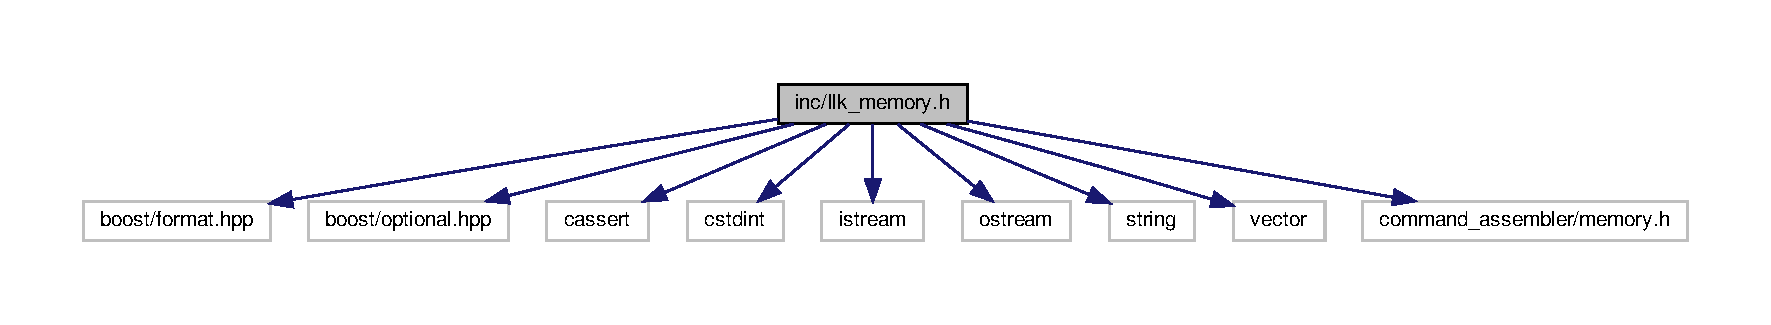
\includegraphics[width=350pt]{llk__memory_8h__incl}
\end{center}
\end{figure}
This graph shows which files directly or indirectly include this file\+:\nopagebreak
\begin{figure}[H]
\begin{center}
\leavevmode
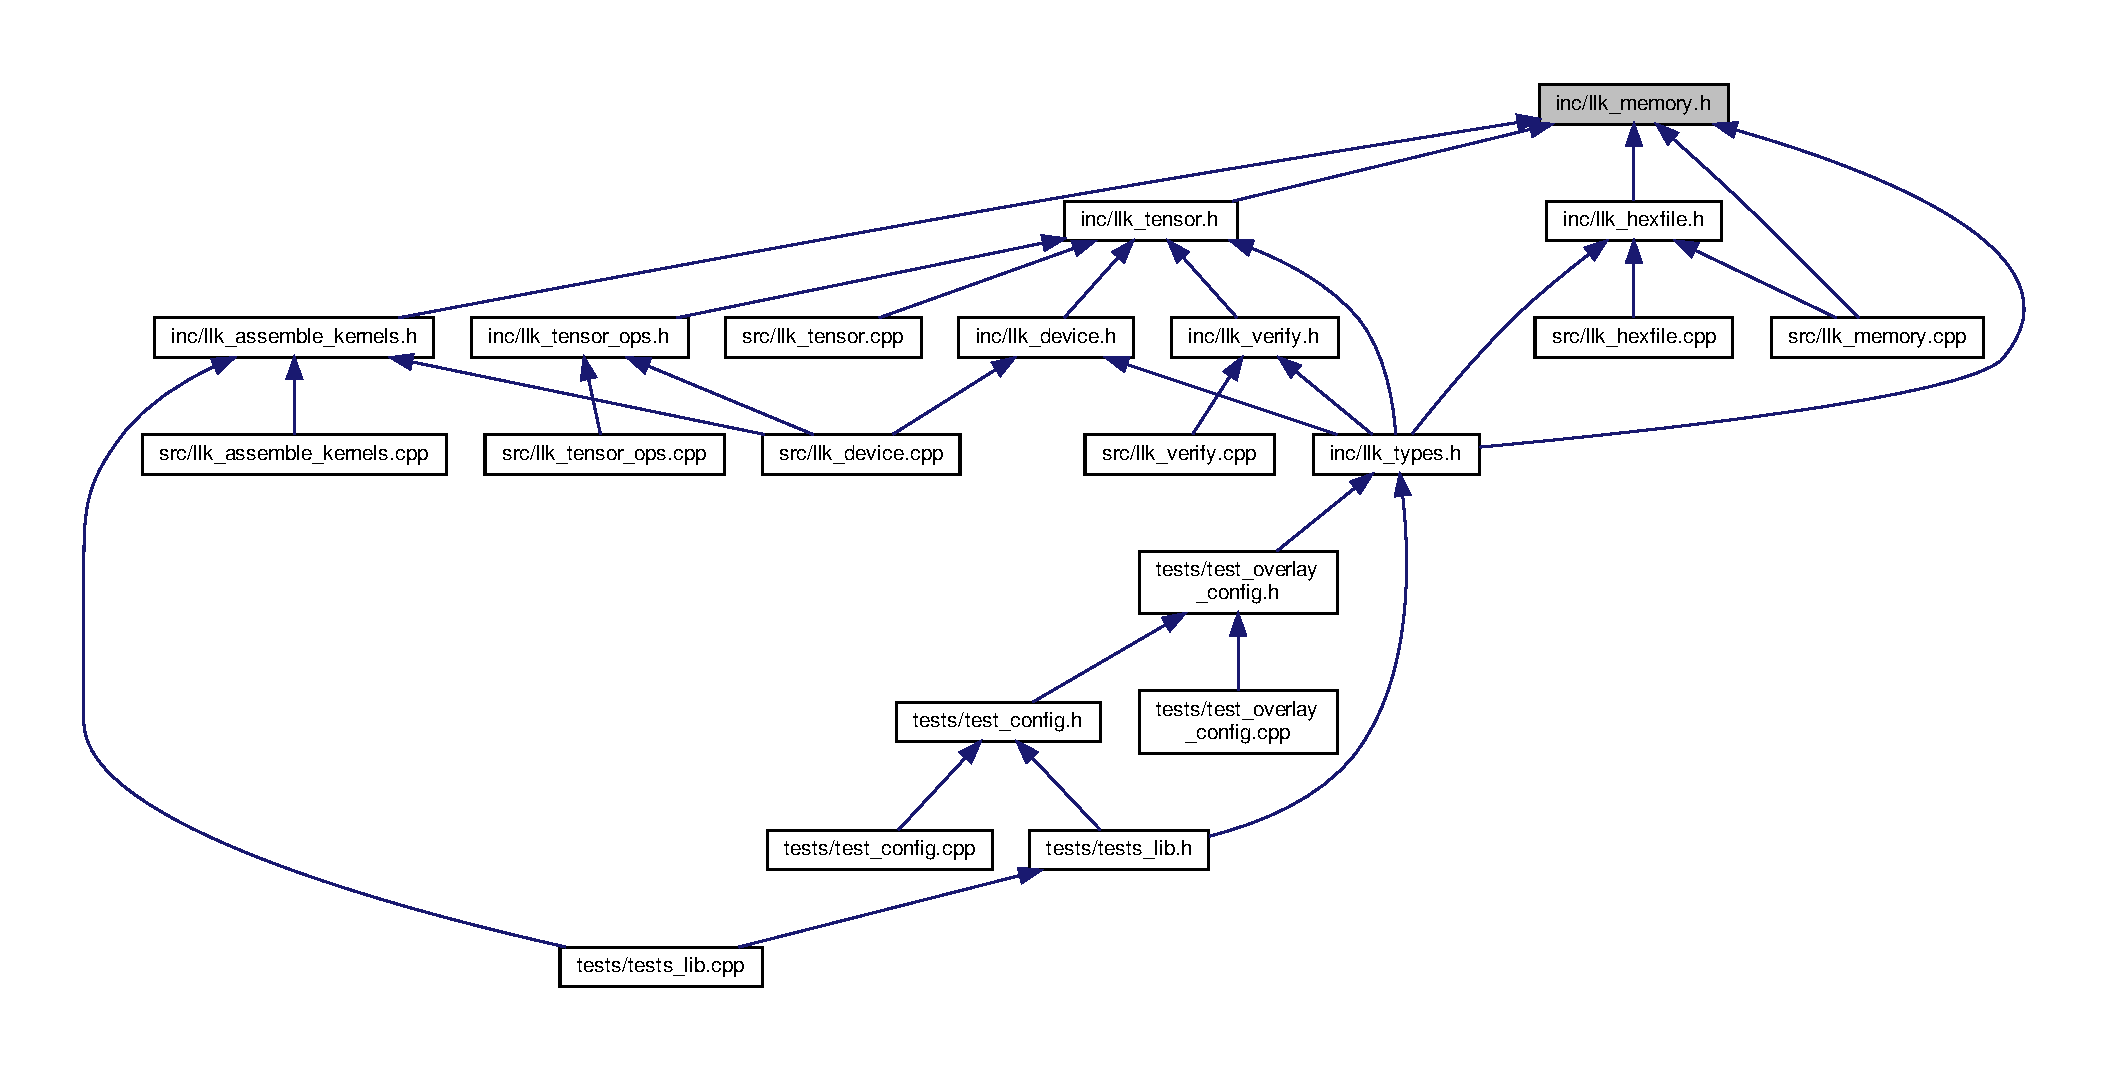
\includegraphics[width=350pt]{llk__memory_8h__dep__incl}
\end{center}
\end{figure}
\subsection*{Classes}
\begin{DoxyCompactItemize}
\item 
class \hyperlink{classllk_1_1memory}{llk\+::memory}
\item 
struct \hyperlink{structllk_1_1BufferMemory}{llk\+::\+Buffer\+Memory}
\end{DoxyCompactItemize}
\subsection*{Namespaces}
\begin{DoxyCompactItemize}
\item 
 \hyperlink{namespacellk}{llk}
\end{DoxyCompactItemize}
\subsection*{Functions}
\begin{DoxyCompactItemize}
\item 
memory\+::address\+\_\+t \hyperlink{namespacellk_af632f3a3bce5453659e5ba431edd703b}{llk\+::\+Write\+Blob} (memory \&mem, memory\+::address\+\_\+t start, const memory\+::word\+\_\+t $\ast$data, long long unsigned count)
\item 
{\footnotesize template$<$typename Span\+Like $>$ }\\auto \hyperlink{namespacellk_a03eaff131f928d8e762175c51ced8fb9}{llk\+::\+Write\+Blob} (memory \&mem, memory\+::address\+\_\+t start, const Span\+Like \&data\+\_\+span)
\item 
memory \hyperlink{namespacellk_adb43fe0eeac466803ff0566f52b4f7a8}{llk\+::slice\+\_\+memory} (const memory \&mem, memory\+::address\+\_\+t base, memory\+::address\+\_\+t start, memory\+::address\+\_\+t end)
\end{DoxyCompactItemize}

\hypertarget{llk__rounding_8h}{}\section{inc/llk\+\_\+rounding.h File Reference}
\label{llk__rounding_8h}\index{inc/llk\+\_\+rounding.\+h@{inc/llk\+\_\+rounding.\+h}}
{\ttfamily \#include $<$cassert$>$}\newline
{\ttfamily \#include $<$limits$>$}\newline
Include dependency graph for llk\+\_\+rounding.\+h\+:\nopagebreak
\begin{figure}[H]
\begin{center}
\leavevmode
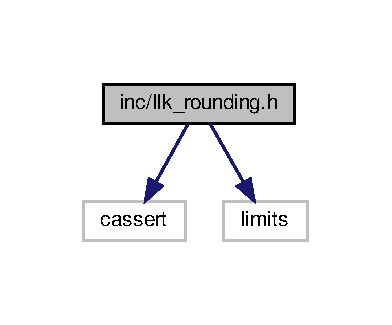
\includegraphics[width=188pt]{llk__rounding_8h__incl}
\end{center}
\end{figure}
This graph shows which files directly or indirectly include this file\+:\nopagebreak
\begin{figure}[H]
\begin{center}
\leavevmode
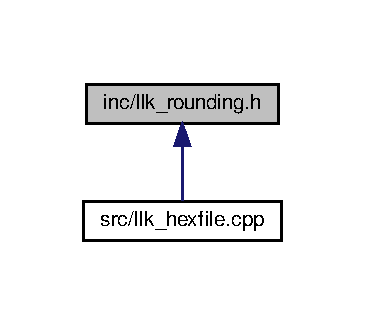
\includegraphics[width=175pt]{llk__rounding_8h__dep__incl}
\end{center}
\end{figure}
\subsection*{Namespaces}
\begin{DoxyCompactItemize}
\item 
 \hyperlink{namespacellk}{llk}
\end{DoxyCompactItemize}
\subsection*{Functions}
\begin{DoxyCompactItemize}
\item 
{\footnotesize template$<$class Integer $>$ }\\constexpr Integer \hyperlink{namespacellk_a8cd09709764d84271aa30cbbdbc8c7dd}{llk\+::round\+\_\+to\+\_\+power\+\_\+of\+\_\+2} (Integer x)
\item 
{\footnotesize template$<$class T , class U $>$ }\\constexpr T \hyperlink{namespacellk_a4d91d6fe231ded1b2eb55d3b804b5da1}{llk\+::round\+\_\+up\+\_\+to} (T x, U multiple)
\item 
{\footnotesize template$<$class T , class U $>$ }\\constexpr T \hyperlink{namespacellk_a3556f6edf607e08801e2cba0f809d09d}{llk\+::round\+\_\+up\+\_\+div} (T dividend, U divisor)
\end{DoxyCompactItemize}

\hypertarget{llk__soc__descriptor_8h}{}\section{inc/llk\+\_\+soc\+\_\+descriptor.h File Reference}
\label{llk__soc__descriptor_8h}\index{inc/llk\+\_\+soc\+\_\+descriptor.\+h@{inc/llk\+\_\+soc\+\_\+descriptor.\+h}}
{\ttfamily \#include $<$cstddef$>$}\newline
{\ttfamily \#include $<$string$>$}\newline
{\ttfamily \#include $<$unordered\+\_\+map$>$}\newline
{\ttfamily \#include $<$vector$>$}\newline
{\ttfamily \#include \char`\"{}llk\+\_\+xy\+\_\+pair.\+h\char`\"{}}\newline
{\ttfamily \#include \char`\"{}yaml-\/cpp/yaml.\+h\char`\"{}}\newline
{\ttfamily \#include \char`\"{}command\+\_\+assembler/soc.\+h\char`\"{}}\newline
Include dependency graph for llk\+\_\+soc\+\_\+descriptor.\+h\+:\nopagebreak
\begin{figure}[H]
\begin{center}
\leavevmode
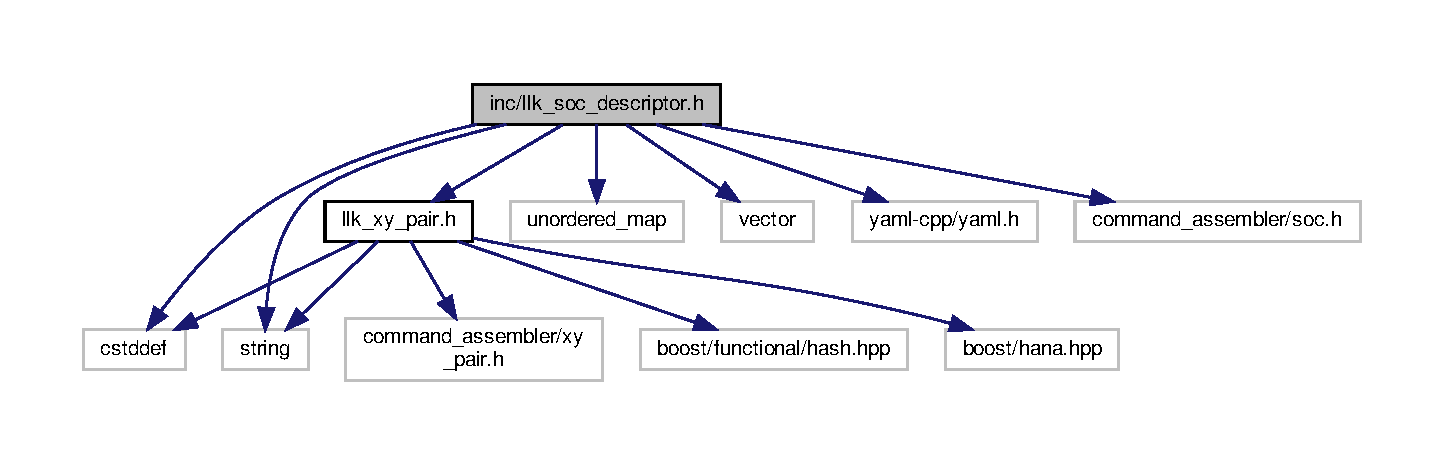
\includegraphics[width=350pt]{llk__soc__descriptor_8h__incl}
\end{center}
\end{figure}
This graph shows which files directly or indirectly include this file\+:\nopagebreak
\begin{figure}[H]
\begin{center}
\leavevmode
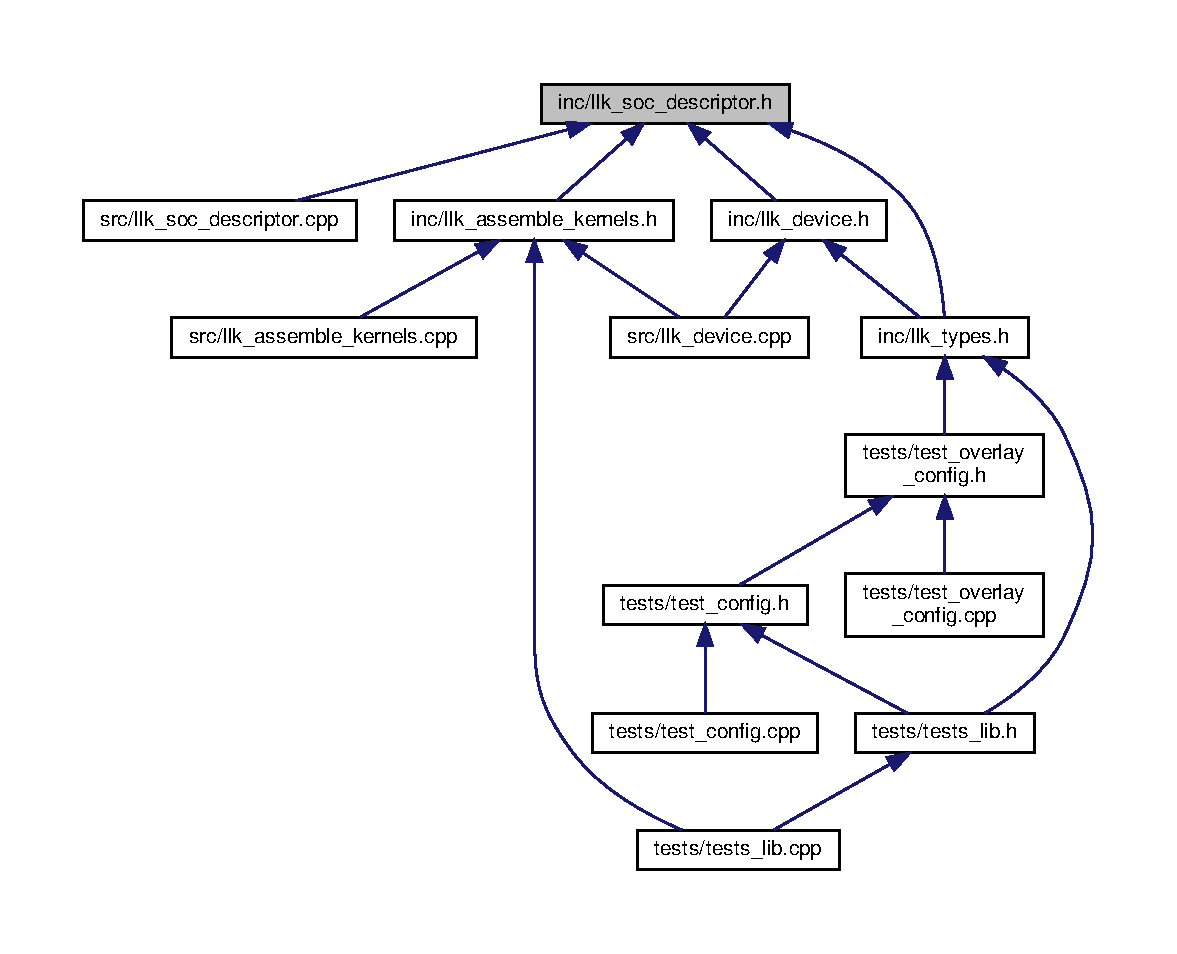
\includegraphics[width=350pt]{llk__soc__descriptor_8h__dep__incl}
\end{center}
\end{figure}
\subsection*{Classes}
\begin{DoxyCompactItemize}
\item 
struct \hyperlink{structllk_1_1CoreDescriptor}{llk\+::\+Core\+Descriptor}
\begin{DoxyCompactList}\small\item\em Soc\+Node\+Descriptor contains information regarding the Node/\+Core. \end{DoxyCompactList}\item 
struct \hyperlink{structllk_1_1SocDescriptor}{llk\+::\+Soc\+Descriptor}
\begin{DoxyCompactList}\small\item\em \hyperlink{structllk_1_1SocDescriptor}{Soc\+Descriptor} contains information regarding the S\+OC configuration targetted. \end{DoxyCompactList}\end{DoxyCompactItemize}
\subsection*{Namespaces}
\begin{DoxyCompactItemize}
\item 
 \hyperlink{namespacellk}{llk}
\end{DoxyCompactItemize}
\subsection*{Enumerations}
\begin{DoxyCompactItemize}
\item 
enum \hyperlink{namespacellk_adb2574c7c85c75a2dfaf60853d0863d2}{llk\+::\+Arch\+Name} \{ \hyperlink{namespacellk_adb2574c7c85c75a2dfaf60853d0863d2afedde270cf558ea8607564b045a78337}{llk\+::\+Arch\+Name\+::\+J\+A\+W\+B\+R\+I\+D\+GE}, 
\hyperlink{namespacellk_adb2574c7c85c75a2dfaf60853d0863d2a876acd7fc1a65f2786b4d75eeed39cbb}{llk\+::\+Arch\+Name\+::\+G\+R\+A\+Y\+S\+K\+U\+LL}, 
\hyperlink{namespacellk_adb2574c7c85c75a2dfaf60853d0863d2ab7cfd894e8bd0e909309ff64bb805fa2}{llk\+::\+Arch\+Name\+::\+W\+O\+R\+M\+H\+O\+LE}
 \}\begin{DoxyCompactList}\small\item\em Arch Enumeration -\/ Chip Generations. \end{DoxyCompactList}
\item 
enum \hyperlink{namespacellk_ad3e730e596589754342a98abd7021ed4}{llk\+::\+Core\+Type} \{ \newline
\hyperlink{namespacellk_ad3e730e596589754342a98abd7021ed4ad72a48a8ebd238e1497a911e938f46e8}{llk\+::\+Core\+Type\+::\+A\+RC}, 
\hyperlink{namespacellk_ad3e730e596589754342a98abd7021ed4aebae17841ce69e653df838d8c20ace8d}{llk\+::\+Core\+Type\+::\+D\+R\+AM}, 
\hyperlink{namespacellk_ad3e730e596589754342a98abd7021ed4af8d2e1584059489f8ffa3663b3223df2}{llk\+::\+Core\+Type\+::\+E\+TH}, 
\hyperlink{namespacellk_ad3e730e596589754342a98abd7021ed4ac0c7fd4fd43dcf7043f237f3819d2863}{llk\+::\+Core\+Type\+::\+P\+C\+IE}, 
\newline
\hyperlink{namespacellk_ad3e730e596589754342a98abd7021ed4a531886e636f1aa36e0fc96d49f342613}{llk\+::\+Core\+Type\+::\+W\+O\+R\+K\+ER}, 
\hyperlink{namespacellk_ad3e730e596589754342a98abd7021ed4a135edd7964c2e277ee73781835c910aa}{llk\+::\+Core\+Type\+::\+H\+A\+R\+V\+E\+S\+T\+ED}, 
\hyperlink{namespacellk_ad3e730e596589754342a98abd7021ed4aa1426080f5aff9d27224e8dd879876c0}{llk\+::\+Core\+Type\+::\+R\+O\+U\+T\+E\+R\+\_\+\+O\+N\+LY}
 \}\begin{DoxyCompactList}\small\item\em Soc\+Core type enumerations. \end{DoxyCompactList}
\end{DoxyCompactItemize}
\subsection*{Functions}
\begin{DoxyCompactItemize}
\item 
const \hyperlink{structllk_1_1SocDescriptor}{llk\+::\+Soc\+Descriptor} \hyperlink{namespacellk_af288472eef4153c0c2592b87940d7e9a}{llk\+::load\+\_\+soc\+\_\+descriptor\+\_\+from\+\_\+yaml} (std\+::string device\+\_\+descriptor\+\_\+file\+\_\+path)
\begin{DoxyCompactList}\small\item\em load\+\_\+soc\+\_\+descriptor\+\_\+from\+\_\+yaml takes a path to yaml and loads the \hyperlink{structllk_1_1SocDescriptor}{llk\+::\+Soc\+Descriptor} with relevant information \end{DoxyCompactList}\item 
void \hyperlink{namespacellk_aba61403c3cbb47767fd66634401ca1ad}{llk\+::load\+\_\+core\+\_\+descriptors\+\_\+from\+\_\+device\+\_\+descriptor} (Y\+A\+M\+L\+::\+Node device\+\_\+descriptor\+\_\+yaml, \hyperlink{structllk_1_1SocDescriptor}{llk\+::\+Soc\+Descriptor} \&soc\+\_\+descriptor)
\item 
void \hyperlink{namespacellk_a15c1d720bf035c008aea9ba25a7150eb}{llk\+::translate\+\_\+soc\+\_\+descriptor\+\_\+to\+\_\+ca\+\_\+soc} (C\+A\+::\+Soc \&soc, const \hyperlink{structllk_1_1SocDescriptor}{llk\+::\+Soc\+Descriptor} soc\+\_\+descriptor)
\begin{DoxyCompactList}\small\item\em translate\+\_\+soc\+\_\+descriptor\+\_\+to\+\_\+ca\+\_\+soc takes a path to yaml and loads the \hyperlink{structllk_1_1SocDescriptor}{llk\+::\+Soc\+Descriptor} with relevant information \end{DoxyCompactList}\end{DoxyCompactItemize}

\hypertarget{llk__tensor_8h}{}\section{inc/llk\+\_\+tensor.h File Reference}
\label{llk__tensor_8h}\index{inc/llk\+\_\+tensor.\+h@{inc/llk\+\_\+tensor.\+h}}
{\ttfamily \#include $<$cstddef$>$}\newline
{\ttfamily \#include $<$iostream$>$}\newline
{\ttfamily \#include $<$sstream$>$}\newline
{\ttfamily \#include $<$string$>$}\newline
{\ttfamily \#include $<$vector$>$}\newline
{\ttfamily \#include \char`\"{}llk\+\_\+memory.\+h\char`\"{}}\newline
{\ttfamily \#include \char`\"{}llk\+\_\+tensor\+\_\+data\+\_\+format.\+h\char`\"{}}\newline
{\ttfamily \#include \char`\"{}llk\+\_\+tensor\+\_\+dims.\+h\char`\"{}}\newline
{\ttfamily \#include \char`\"{}llk\+\_\+tensor\+\_\+tile\+\_\+layout.\+h\char`\"{}}\newline
{\ttfamily \#include \char`\"{}llk\+\_\+xy\+\_\+pair.\+h\char`\"{}}\newline
{\ttfamily \#include \char`\"{}tile.\+h\char`\"{}}\newline
{\ttfamily \#include \char`\"{}utils/math.\+h\char`\"{}}\newline
Include dependency graph for llk\+\_\+tensor.\+h\+:\nopagebreak
\begin{figure}[H]
\begin{center}
\leavevmode
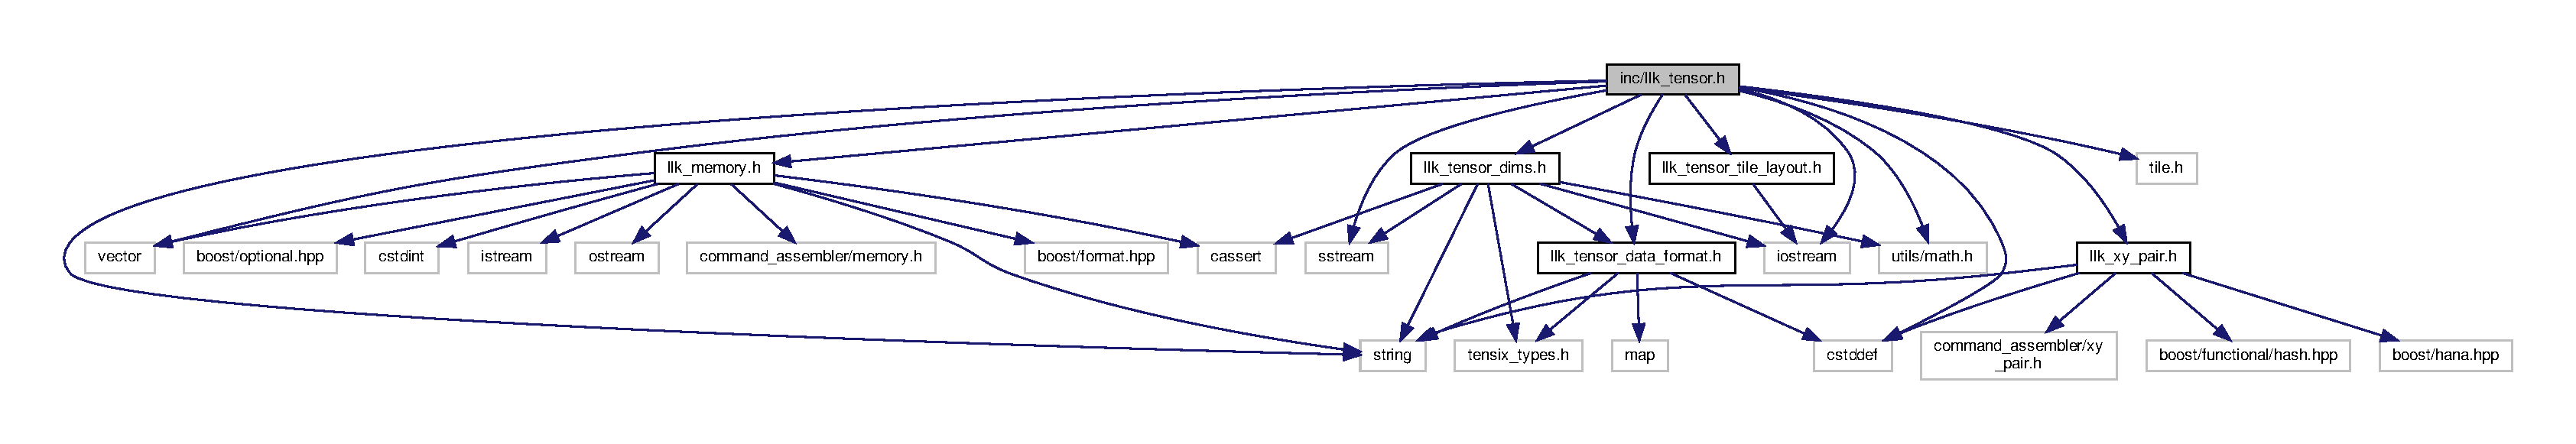
\includegraphics[width=350pt]{llk__tensor_8h__incl}
\end{center}
\end{figure}
This graph shows which files directly or indirectly include this file\+:\nopagebreak
\begin{figure}[H]
\begin{center}
\leavevmode
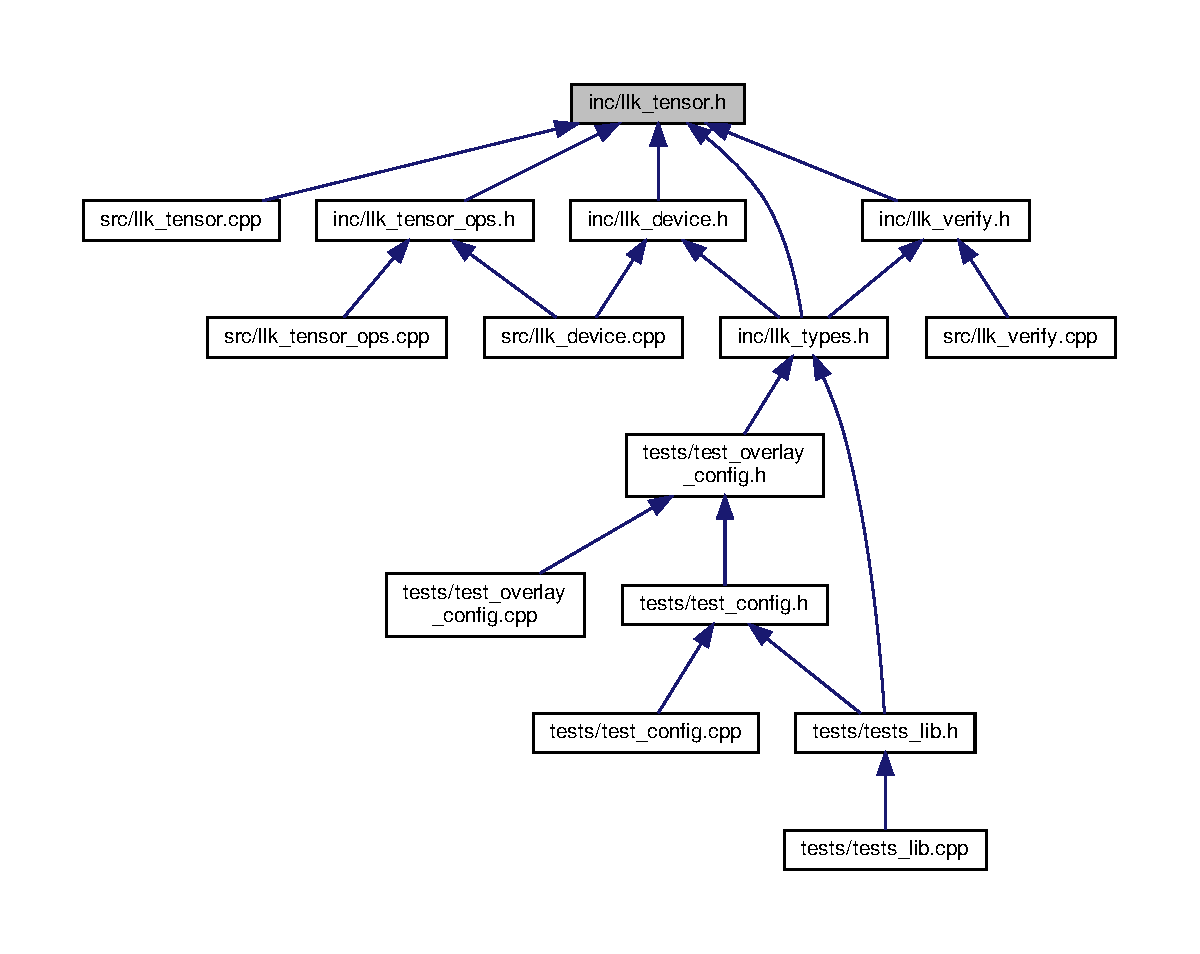
\includegraphics[width=350pt]{llk__tensor_8h__dep__incl}
\end{center}
\end{figure}
\subsection*{Classes}
\begin{DoxyCompactItemize}
\item 
class \hyperlink{classllk_1_1Tensor}{llk\+::\+Tensor}
\end{DoxyCompactItemize}
\subsection*{Namespaces}
\begin{DoxyCompactItemize}
\item 
 \hyperlink{namespacellk}{llk}
\end{DoxyCompactItemize}

\hypertarget{llk__tensor__data__format_8h}{}\section{inc/llk\+\_\+tensor\+\_\+data\+\_\+format.h File Reference}
\label{llk__tensor__data__format_8h}\index{inc/llk\+\_\+tensor\+\_\+data\+\_\+format.\+h@{inc/llk\+\_\+tensor\+\_\+data\+\_\+format.\+h}}
{\ttfamily \#include $<$cstddef$>$}\newline
{\ttfamily \#include $<$map$>$}\newline
{\ttfamily \#include $<$string$>$}\newline
{\ttfamily \#include \char`\"{}tensix\+\_\+types.\+h\char`\"{}}\newline
Include dependency graph for llk\+\_\+tensor\+\_\+data\+\_\+format.\+h\+:\nopagebreak
\begin{figure}[H]
\begin{center}
\leavevmode
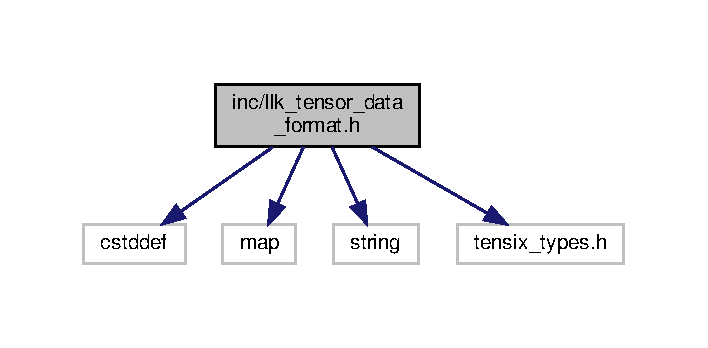
\includegraphics[width=340pt]{llk__tensor__data__format_8h__incl}
\end{center}
\end{figure}
This graph shows which files directly or indirectly include this file\+:\nopagebreak
\begin{figure}[H]
\begin{center}
\leavevmode
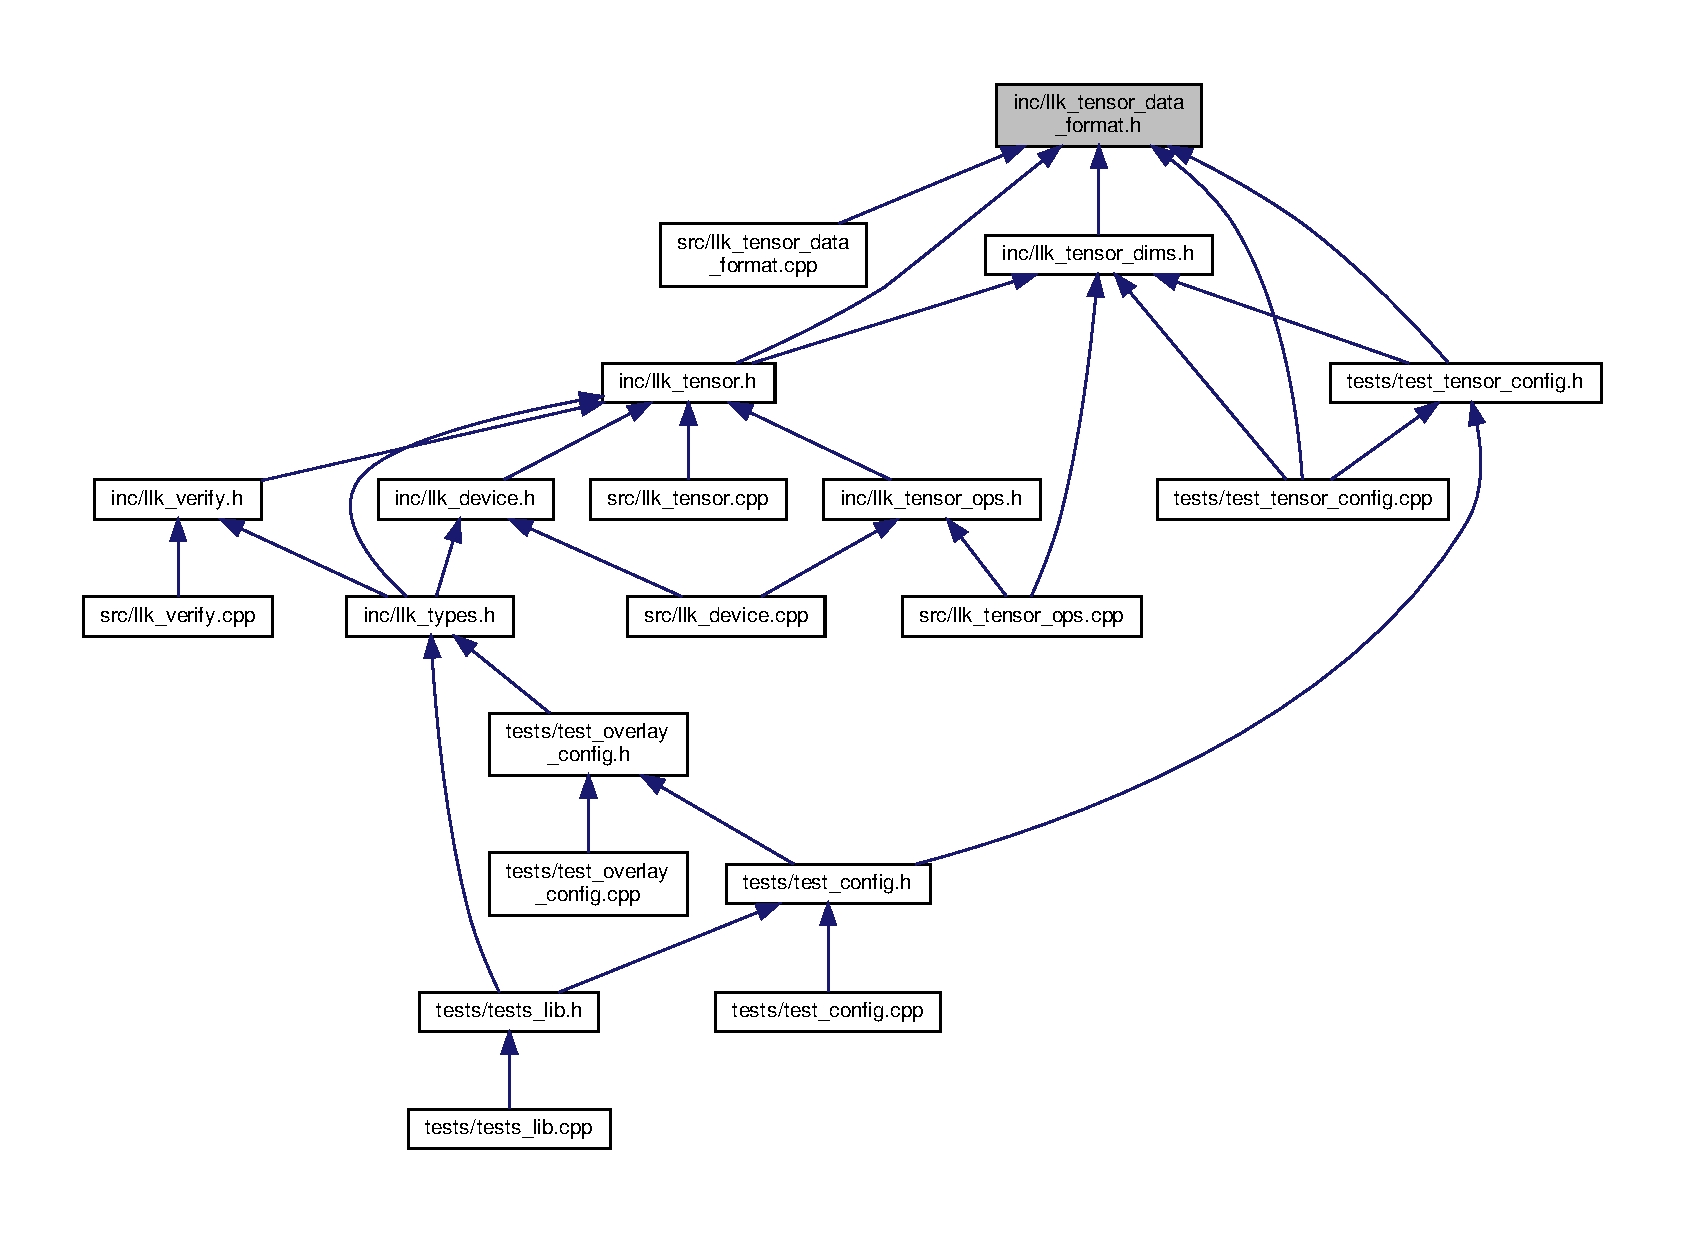
\includegraphics[width=350pt]{llk__tensor__data__format_8h__dep__incl}
\end{center}
\end{figure}
\subsection*{Namespaces}
\begin{DoxyCompactItemize}
\item 
 \hyperlink{namespacellk}{llk}
\end{DoxyCompactItemize}
\subsection*{Functions}
\begin{DoxyCompactItemize}
\item 
std\+::string \hyperlink{namespacellk_a7477ba6804f7b1d71805930f84bfe85f}{llk\+::to\+\_\+str} (const Data\+Format in\+Type)
\item 
Data\+Format \hyperlink{namespacellk_a4d05986053a0ef31039cf648d9b673f9}{llk\+::get\+\_\+data\+\_\+format} (const std\+::string in\+\_\+data\+\_\+format)
\item 
int \hyperlink{namespacellk_aede7298fde3871110bbe72268aeac557}{llk\+::num\+\_\+bytes} (const Data\+Format in\+Type)
\item 
int \hyperlink{namespacellk_ad38ed2c0bc96eb57b9141ec67ae3988a}{llk\+::num\+\_\+bytes\+\_\+extra} (const Data\+Format in\+Type)
\end{DoxyCompactItemize}

\hypertarget{llk__tensor__dims_8h}{}\section{inc/llk\+\_\+tensor\+\_\+dims.h File Reference}
\label{llk__tensor__dims_8h}\index{inc/llk\+\_\+tensor\+\_\+dims.\+h@{inc/llk\+\_\+tensor\+\_\+dims.\+h}}
{\ttfamily \#include $<$cassert$>$}\newline
{\ttfamily \#include $<$iostream$>$}\newline
{\ttfamily \#include $<$sstream$>$}\newline
{\ttfamily \#include $<$string$>$}\newline
{\ttfamily \#include \char`\"{}llk\+\_\+tensor\+\_\+data\+\_\+format.\+h\char`\"{}}\newline
{\ttfamily \#include \char`\"{}tensix\+\_\+types.\+h\char`\"{}}\newline
{\ttfamily \#include \char`\"{}utils/math.\+h\char`\"{}}\newline
Include dependency graph for llk\+\_\+tensor\+\_\+dims.\+h\+:\nopagebreak
\begin{figure}[H]
\begin{center}
\leavevmode
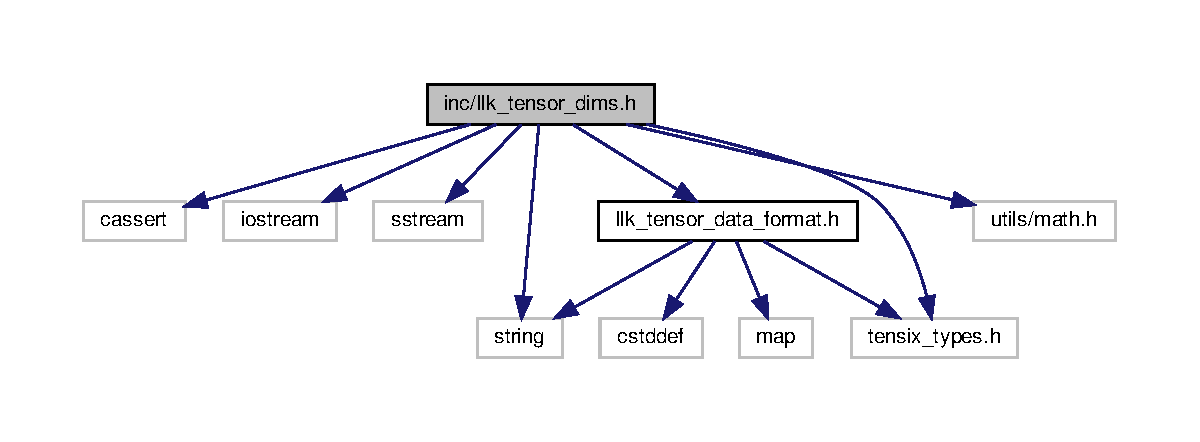
\includegraphics[width=350pt]{llk__tensor__dims_8h__incl}
\end{center}
\end{figure}
This graph shows which files directly or indirectly include this file\+:\nopagebreak
\begin{figure}[H]
\begin{center}
\leavevmode
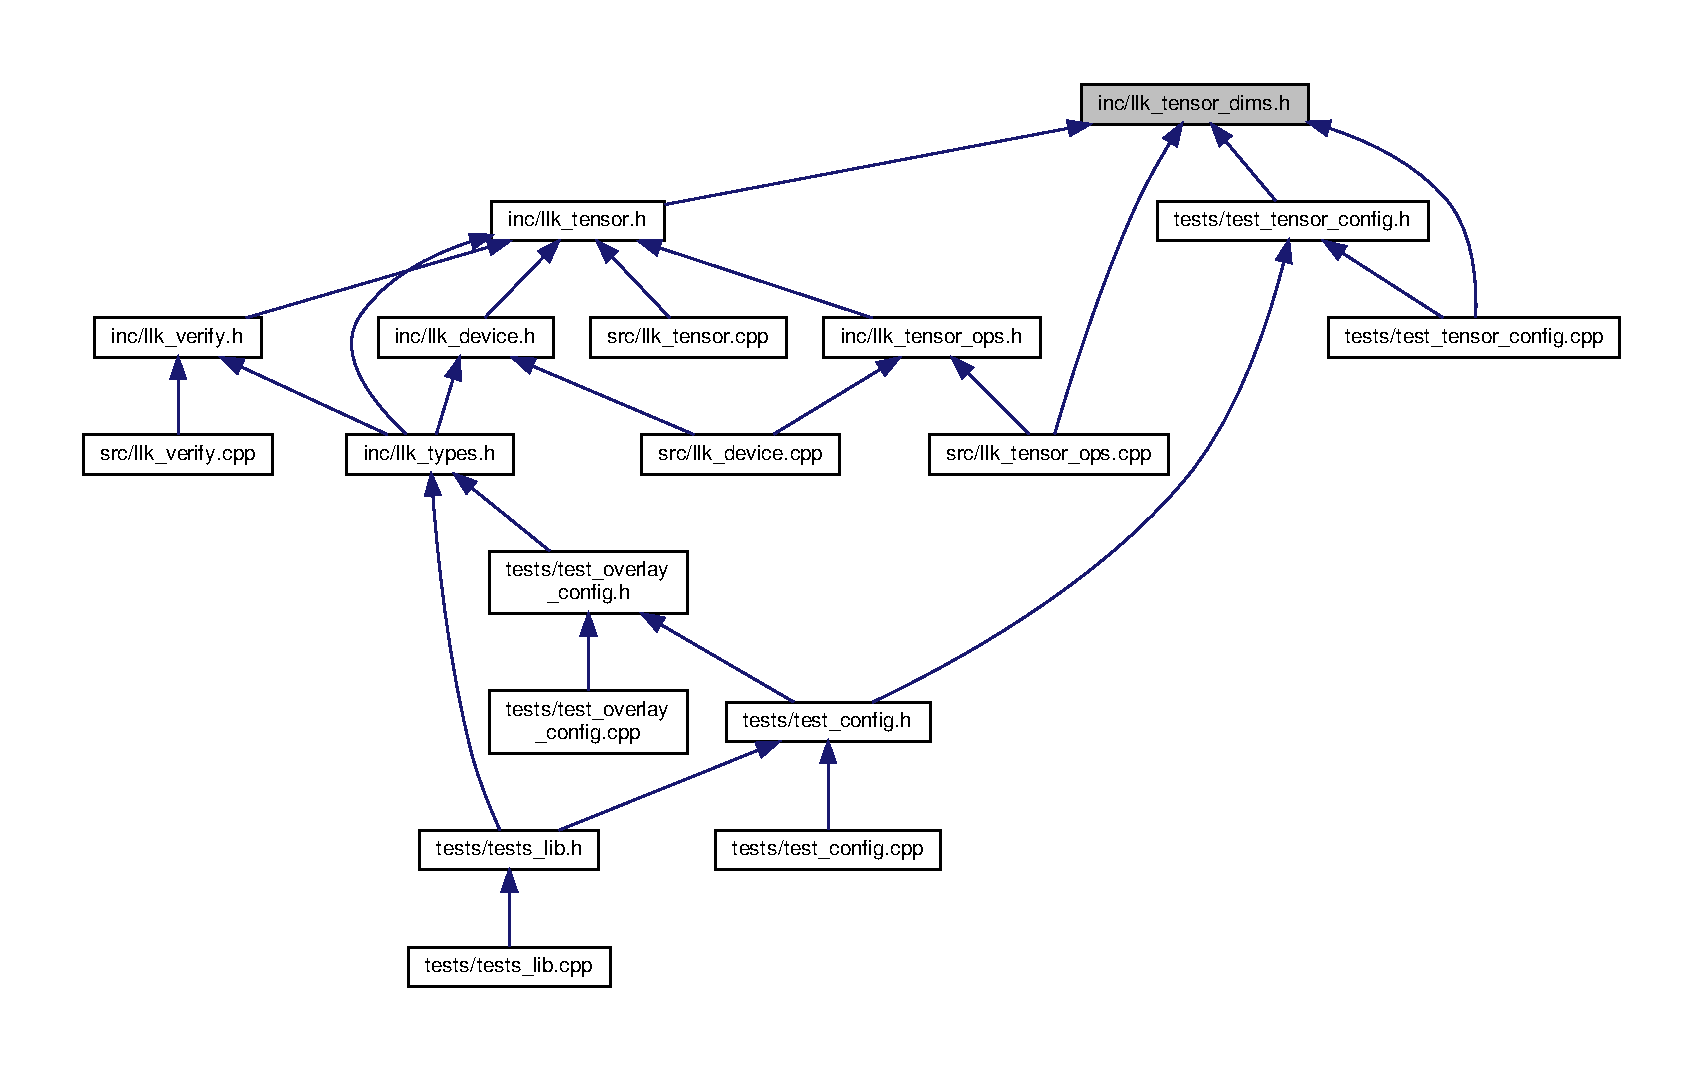
\includegraphics[width=350pt]{llk__tensor__dims_8h__dep__incl}
\end{center}
\end{figure}
\subsection*{Classes}
\begin{DoxyCompactItemize}
\item 
struct \hyperlink{structllk_1_1TensorDims}{llk\+::\+Tensor\+Dims}
\end{DoxyCompactItemize}
\subsection*{Namespaces}
\begin{DoxyCompactItemize}
\item 
 \hyperlink{namespacellk}{llk}
\end{DoxyCompactItemize}

\hypertarget{llk__tensor__ops_8h}{}\section{inc/llk\+\_\+tensor\+\_\+ops.h File Reference}
\label{llk__tensor__ops_8h}\index{inc/llk\+\_\+tensor\+\_\+ops.\+h@{inc/llk\+\_\+tensor\+\_\+ops.\+h}}
{\ttfamily \#include $<$string$>$}\newline
{\ttfamily \#include $<$unordered\+\_\+map$>$}\newline
{\ttfamily \#include \char`\"{}llk\+\_\+tensor.\+h\char`\"{}}\newline
Include dependency graph for llk\+\_\+tensor\+\_\+ops.\+h\+:\nopagebreak
\begin{figure}[H]
\begin{center}
\leavevmode
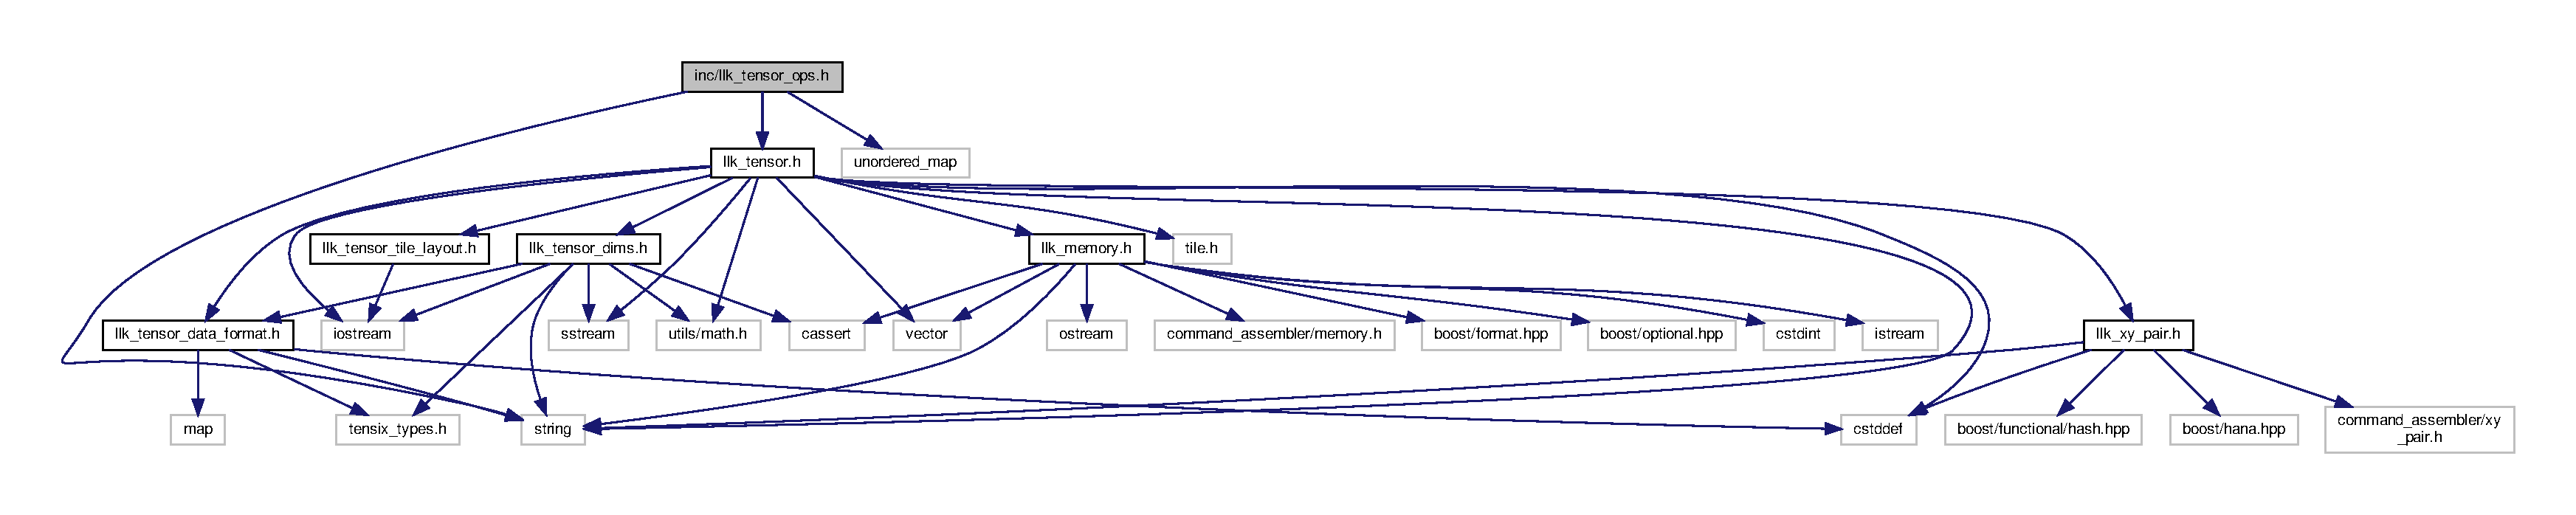
\includegraphics[width=350pt]{llk__tensor__ops_8h__incl}
\end{center}
\end{figure}
This graph shows which files directly or indirectly include this file\+:\nopagebreak
\begin{figure}[H]
\begin{center}
\leavevmode
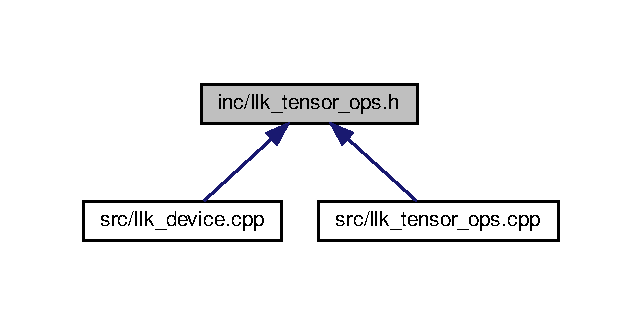
\includegraphics[width=308pt]{llk__tensor__ops_8h__dep__incl}
\end{center}
\end{figure}
\subsection*{Namespaces}
\begin{DoxyCompactItemize}
\item 
 \hyperlink{namespacellk}{llk}
\item 
 \hyperlink{namespacellk_1_1tensor__ops}{llk\+::tensor\+\_\+ops}
\item 
 \hyperlink{namespacellk_1_1tensor__ops_1_1tile__ops}{llk\+::tensor\+\_\+ops\+::tile\+\_\+ops}
\end{DoxyCompactItemize}
\subsection*{Enumerations}
\begin{DoxyCompactItemize}
\item 
enum \hyperlink{namespacellk_1_1tensor__ops_ac43a7c3eb367c669baaa45a327aeca58}{llk\+::tensor\+\_\+ops\+::broadcast\+\_\+op} \{ \hyperlink{namespacellk_1_1tensor__ops_ac43a7c3eb367c669baaa45a327aeca58ab50339a10e1de285ac99d4c3990b8693}{llk\+::tensor\+\_\+ops\+::broadcast\+\_\+op\+::\+N\+O\+NE}, 
\hyperlink{namespacellk_1_1tensor__ops_ac43a7c3eb367c669baaa45a327aeca58aa44a065875f5d66d41474bb9bfb0ce05}{llk\+::tensor\+\_\+ops\+::broadcast\+\_\+op\+::\+C\+OL}, 
\hyperlink{namespacellk_1_1tensor__ops_ac43a7c3eb367c669baaa45a327aeca58a54c1ed33c810f895d48c008d89f880b7}{llk\+::tensor\+\_\+ops\+::broadcast\+\_\+op\+::\+R\+OW}, 
\hyperlink{namespacellk_1_1tensor__ops_ac43a7c3eb367c669baaa45a327aeca58a8f3d9a4b6a7b7f2c7afa61ca113d0db9}{llk\+::tensor\+\_\+ops\+::broadcast\+\_\+op\+::\+S\+C\+A\+L\+AR}
 \}
\item 
enum \hyperlink{namespacellk_1_1tensor__ops_a255b8a4e49bc956c2731c62bf613c0f8}{llk\+::tensor\+\_\+ops\+::binary\+\_\+op} \{ \hyperlink{namespacellk_1_1tensor__ops_a255b8a4e49bc956c2731c62bf613c0f8a7eae59e4ffdb2f42b7f9cce2b4a8380b}{llk\+::tensor\+\_\+ops\+::binary\+\_\+op\+::\+E\+L\+W\+A\+DD}, 
\hyperlink{namespacellk_1_1tensor__ops_a255b8a4e49bc956c2731c62bf613c0f8ae7b63c46c106f75a7763346466e64f17}{llk\+::tensor\+\_\+ops\+::binary\+\_\+op\+::\+E\+L\+W\+S\+UB}, 
\hyperlink{namespacellk_1_1tensor__ops_a255b8a4e49bc956c2731c62bf613c0f8a96833ad817e8282b9b30ce6d82f4cecb}{llk\+::tensor\+\_\+ops\+::binary\+\_\+op\+::\+E\+L\+W\+M\+UL}, 
\hyperlink{namespacellk_1_1tensor__ops_a255b8a4e49bc956c2731c62bf613c0f8aa29508ee97e8cec04526b5572bde54c2}{llk\+::tensor\+\_\+ops\+::binary\+\_\+op\+::\+E\+L\+W\+D\+IV}
 \}
\item 
enum \hyperlink{namespacellk_1_1tensor__ops_a5fae70cbcf6cd7aadca4a04278614633}{llk\+::tensor\+\_\+ops\+::unary\+\_\+op} \{ \newline
\hyperlink{namespacellk_1_1tensor__ops_a5fae70cbcf6cd7aadca4a04278614633a4e8ae44bfa6130cf30eeea9ec96b2b16}{llk\+::tensor\+\_\+ops\+::unary\+\_\+op\+::\+D\+A\+T\+A\+C\+O\+PY}, 
\hyperlink{namespacellk_1_1tensor__ops_a5fae70cbcf6cd7aadca4a04278614633adcd5fc33e211f31cef0cd7cb36518d31}{llk\+::tensor\+\_\+ops\+::unary\+\_\+op\+::\+E\+X\+P\+O\+N\+E\+N\+T\+I\+AL}, 
\hyperlink{namespacellk_1_1tensor__ops_a5fae70cbcf6cd7aadca4a04278614633a6c83d4d579e33c2e1b09f2e9825fcbc6}{llk\+::tensor\+\_\+ops\+::unary\+\_\+op\+::\+G\+E\+LU}, 
\hyperlink{namespacellk_1_1tensor__ops_a5fae70cbcf6cd7aadca4a04278614633a4b5ffcdaf38ce4d463171f5c977c5ab3}{llk\+::tensor\+\_\+ops\+::unary\+\_\+op\+::\+L\+OG}, 
\newline
\hyperlink{namespacellk_1_1tensor__ops_a5fae70cbcf6cd7aadca4a04278614633a4d98346f3d5cc5fa5666f0715abf25b1}{llk\+::tensor\+\_\+ops\+::unary\+\_\+op\+::\+R\+E\+C\+I\+P\+R\+O\+C\+AL}, 
\hyperlink{namespacellk_1_1tensor__ops_a5fae70cbcf6cd7aadca4a04278614633a36875f2500a09ee35d0bb7eb8c0b91b0}{llk\+::tensor\+\_\+ops\+::unary\+\_\+op\+::\+S\+Q\+RT}, 
\hyperlink{namespacellk_1_1tensor__ops_a5fae70cbcf6cd7aadca4a04278614633a143c8c6f51b9bb893ce71e38702e3cc1}{llk\+::tensor\+\_\+ops\+::unary\+\_\+op\+::\+T\+A\+NH}, 
\hyperlink{namespacellk_1_1tensor__ops_a5fae70cbcf6cd7aadca4a04278614633a053f0427225784e44f53963788455e4b}{llk\+::tensor\+\_\+ops\+::unary\+\_\+op\+::\+T\+R\+A\+N\+S\+P\+O\+S\+E\+\_\+\+XY}
 \}
\item 
enum \hyperlink{namespacellk_1_1tensor__ops_abbf479560e4c31bec0b83feb6531552c}{llk\+::tensor\+\_\+ops\+::reduce\+\_\+math\+\_\+op} \{ \hyperlink{namespacellk_1_1tensor__ops_abbf479560e4c31bec0b83feb6531552cafcefd647d6a866603c627b11347c707a}{llk\+::tensor\+\_\+ops\+::reduce\+\_\+math\+\_\+op\+::\+A\+VG}, 
\hyperlink{namespacellk_1_1tensor__ops_abbf479560e4c31bec0b83feb6531552ca26a4b44a837bf97b972628509912b4a5}{llk\+::tensor\+\_\+ops\+::reduce\+\_\+math\+\_\+op\+::\+M\+AX}, 
\hyperlink{namespacellk_1_1tensor__ops_abbf479560e4c31bec0b83feb6531552ca6970bdc2201030b9c03fbdcf3973858a}{llk\+::tensor\+\_\+ops\+::reduce\+\_\+math\+\_\+op\+::\+S\+UM}
 \}
\item 
enum \hyperlink{namespacellk_1_1tensor__ops_a57720b85adbe1e9b3bbab02b985f0d8d}{llk\+::tensor\+\_\+ops\+::reduce\+\_\+op} \{ \hyperlink{namespacellk_1_1tensor__ops_a57720b85adbe1e9b3bbab02b985f0d8da54c1ed33c810f895d48c008d89f880b7}{llk\+::tensor\+\_\+ops\+::reduce\+\_\+op\+::\+R\+OW}, 
\hyperlink{namespacellk_1_1tensor__ops_a57720b85adbe1e9b3bbab02b985f0d8daa44a065875f5d66d41474bb9bfb0ce05}{llk\+::tensor\+\_\+ops\+::reduce\+\_\+op\+::\+C\+OL}, 
\hyperlink{namespacellk_1_1tensor__ops_a57720b85adbe1e9b3bbab02b985f0d8da8f3d9a4b6a7b7f2c7afa61ca113d0db9}{llk\+::tensor\+\_\+ops\+::reduce\+\_\+op\+::\+S\+C\+A\+L\+AR}
 \}
\item 
enum \hyperlink{namespacellk_1_1tensor__ops_a3a9aca203c5d38260a1dd35253d57ee8}{llk\+::tensor\+\_\+ops\+::transpose\+\_\+op} \{ \hyperlink{namespacellk_1_1tensor__ops_a3a9aca203c5d38260a1dd35253d57ee8a74c53bcd3dcb2bb79993b2fec37d362a}{llk\+::tensor\+\_\+ops\+::transpose\+\_\+op\+::\+XY}, 
\hyperlink{namespacellk_1_1tensor__ops_a3a9aca203c5d38260a1dd35253d57ee8affa4ba973372c3650fd0881abeca6512}{llk\+::tensor\+\_\+ops\+::transpose\+\_\+op\+::\+YZ}
 \}
\end{DoxyCompactItemize}
\subsection*{Functions}
\begin{DoxyCompactItemize}
\item 
\hyperlink{namespacellk_1_1tensor__ops_ac43a7c3eb367c669baaa45a327aeca58}{broadcast\+\_\+op} \hyperlink{namespacellk_1_1tensor__ops_ae8a576b0f24c7afb92b7e4b22661cd1b}{llk\+::tensor\+\_\+ops\+::get\+\_\+broadcast\+\_\+op\+\_\+from\+\_\+string} (std\+::string op\+\_\+string)
\item 
\hyperlink{namespacellk_1_1tensor__ops_a255b8a4e49bc956c2731c62bf613c0f8}{binary\+\_\+op} \hyperlink{namespacellk_1_1tensor__ops_a6ec11e5d6ad65a752a7464184a8f0b6e}{llk\+::tensor\+\_\+ops\+::get\+\_\+binary\+\_\+op\+\_\+from\+\_\+string} (std\+::string op\+\_\+string)
\item 
\hyperlink{namespacellk_1_1tensor__ops_a5fae70cbcf6cd7aadca4a04278614633}{unary\+\_\+op} \hyperlink{namespacellk_1_1tensor__ops_afb8428deeda6bd3a1a0f2ff7518bc5fa}{llk\+::tensor\+\_\+ops\+::get\+\_\+unary\+\_\+op\+\_\+from\+\_\+string} (std\+::string op\+\_\+string)
\item 
\hyperlink{namespacellk_1_1tensor__ops_abbf479560e4c31bec0b83feb6531552c}{reduce\+\_\+math\+\_\+op} \hyperlink{namespacellk_1_1tensor__ops_ae952831458460f89fe2cca8d82f7334b}{llk\+::tensor\+\_\+ops\+::get\+\_\+reduce\+\_\+math\+\_\+op\+\_\+from\+\_\+string} (std\+::string op\+\_\+string)
\item 
\hyperlink{namespacellk_1_1tensor__ops_a57720b85adbe1e9b3bbab02b985f0d8d}{reduce\+\_\+op} \hyperlink{namespacellk_1_1tensor__ops_afcefdc3151ece6e39e2cb451268e85ac}{llk\+::tensor\+\_\+ops\+::get\+\_\+reduce\+\_\+op\+\_\+from\+\_\+string} (std\+::string op\+\_\+string)
\item 
\hyperlink{namespacellk_1_1tensor__ops_a3a9aca203c5d38260a1dd35253d57ee8}{transpose\+\_\+op} \hyperlink{namespacellk_1_1tensor__ops_af559d533a9e952194483605bfd11d59e}{llk\+::tensor\+\_\+ops\+::get\+\_\+transpose\+\_\+op\+\_\+from\+\_\+string} (std\+::string op\+\_\+string)
\item 
void \hyperlink{namespacellk_1_1tensor__ops_a95e1bfff1cd795053d5686fd418213e8}{llk\+::tensor\+\_\+ops\+::broadcast} (\hyperlink{namespacellk_1_1tensor__ops_ac43a7c3eb367c669baaa45a327aeca58}{broadcast\+\_\+op} op\+\_\+type, \hyperlink{classllk_1_1Tensor}{llk\+::\+Tensor} \&dst, \hyperlink{structllk_1_1TensorDims}{llk\+::\+Tensor\+Dims} dst\+\_\+dims, \hyperlink{classllk_1_1Tensor}{llk\+::\+Tensor} \&src)
\begin{DoxyCompactList}\small\item\em Broadcast \hyperlink{classllk_1_1Tensor}{Tensor} operation -- dst = broadcast(src) \end{DoxyCompactList}\item 
void \hyperlink{namespacellk_1_1tensor__ops_a9727143b8fd7719345cbfd05a3fafb35}{llk\+::tensor\+\_\+ops\+::unary} (\hyperlink{namespacellk_1_1tensor__ops_a5fae70cbcf6cd7aadca4a04278614633}{unary\+\_\+op} op\+\_\+type, \hyperlink{classllk_1_1Tensor}{llk\+::\+Tensor} \&dst, \hyperlink{classllk_1_1Tensor}{llk\+::\+Tensor} \&src)
\begin{DoxyCompactList}\small\item\em Unary operation -- dst = unary(src) \end{DoxyCompactList}\item 
void \hyperlink{namespacellk_1_1tensor__ops_a4430dd9c877f3b6fef3fd296131db096}{llk\+::tensor\+\_\+ops\+::unary\+\_\+broadcast} (\hyperlink{namespacellk_1_1tensor__ops_a5fae70cbcf6cd7aadca4a04278614633}{unary\+\_\+op} op\+\_\+type, \hyperlink{classllk_1_1Tensor}{llk\+::\+Tensor} \&dst, \hyperlink{structllk_1_1TensorDims}{llk\+::\+Tensor\+Dims} dst\+\_\+dims, \hyperlink{classllk_1_1Tensor}{llk\+::\+Tensor} \&src, \hyperlink{namespacellk_1_1tensor__ops_ac43a7c3eb367c669baaa45a327aeca58}{broadcast\+\_\+op} src\+\_\+broadcast\+\_\+type)
\begin{DoxyCompactList}\small\item\em Broadcast Unary operation -- dst = src. \end{DoxyCompactList}\item 
void \hyperlink{namespacellk_1_1tensor__ops_a97daba7fed93172c04f78497d2513e77}{llk\+::tensor\+\_\+ops\+::binary} (\hyperlink{namespacellk_1_1tensor__ops_a255b8a4e49bc956c2731c62bf613c0f8}{binary\+\_\+op} op\+\_\+type, \hyperlink{classllk_1_1Tensor}{llk\+::\+Tensor} \&dst, \hyperlink{classllk_1_1Tensor}{llk\+::\+Tensor} \&src1, \hyperlink{classllk_1_1Tensor}{llk\+::\+Tensor} \&src2)
\begin{DoxyCompactList}\small\item\em Binary operation -- dst = src1 $<$op$>$ src2. \end{DoxyCompactList}\item 
void \hyperlink{namespacellk_1_1tensor__ops_aecac6c5bbeaf3abf3e5a3c7e325728bc}{llk\+::tensor\+\_\+ops\+::binary\+\_\+broadcast} (\hyperlink{namespacellk_1_1tensor__ops_a255b8a4e49bc956c2731c62bf613c0f8}{binary\+\_\+op} op\+\_\+type, \hyperlink{classllk_1_1Tensor}{llk\+::\+Tensor} \&dst, \hyperlink{structllk_1_1TensorDims}{llk\+::\+Tensor\+Dims} dst\+\_\+dims, \hyperlink{classllk_1_1Tensor}{llk\+::\+Tensor} \&src1, \hyperlink{namespacellk_1_1tensor__ops_ac43a7c3eb367c669baaa45a327aeca58}{broadcast\+\_\+op} src1\+\_\+broadcast\+\_\+type, \hyperlink{classllk_1_1Tensor}{llk\+::\+Tensor} \&src2, \hyperlink{namespacellk_1_1tensor__ops_ac43a7c3eb367c669baaa45a327aeca58}{broadcast\+\_\+op} src2\+\_\+broadcast\+\_\+type)
\begin{DoxyCompactList}\small\item\em Broadcast Binary operation -- dst = src1 $<$op$>$ src2. \end{DoxyCompactList}\item 
void \hyperlink{namespacellk_1_1tensor__ops_a4804848e756700934cfe20be8565265c}{llk\+::tensor\+\_\+ops\+::reduce} (\hyperlink{namespacellk_1_1tensor__ops_a57720b85adbe1e9b3bbab02b985f0d8d}{reduce\+\_\+op} op\+\_\+type, \hyperlink{namespacellk_1_1tensor__ops_abbf479560e4c31bec0b83feb6531552c}{reduce\+\_\+math\+\_\+op} math\+\_\+op\+\_\+type, \hyperlink{classllk_1_1Tensor}{llk\+::\+Tensor} \&dst, \hyperlink{classllk_1_1Tensor}{llk\+::\+Tensor} \&src, float multiplier)
\begin{DoxyCompactList}\small\item\em Row Pool Operation. \end{DoxyCompactList}\item 
void \hyperlink{namespacellk_1_1tensor__ops_adcbf09725b122e136e6fc4f90c34a909}{llk\+::tensor\+\_\+ops\+::matmul} (\hyperlink{classllk_1_1Tensor}{llk\+::\+Tensor} \&dst, \hyperlink{classllk_1_1Tensor}{llk\+::\+Tensor} \&src1, \hyperlink{classllk_1_1Tensor}{llk\+::\+Tensor} \&src2)
\begin{DoxyCompactList}\small\item\em Matmul operation -- dst = src1 $<$op$>$ src2. \end{DoxyCompactList}\item 
void \hyperlink{namespacellk_1_1tensor__ops_ad76f0782652afbdf1f6032e44cae4288}{llk\+::tensor\+\_\+ops\+::pack} (\hyperlink{classllk_1_1Tensor}{llk\+::\+Tensor} \&dst, \hyperlink{classllk_1_1Tensor}{llk\+::\+Tensor} \&src)
\begin{DoxyCompactList}\small\item\em Pack operation -- assumes src is unpacked and float tiles. dst = pack(src) \end{DoxyCompactList}\item 
void \hyperlink{namespacellk_1_1tensor__ops_a2aba5bcddb604c8d7fad329330782df4}{llk\+::tensor\+\_\+ops\+::unpack} (\hyperlink{classllk_1_1Tensor}{llk\+::\+Tensor} \&dst, \hyperlink{classllk_1_1Tensor}{llk\+::\+Tensor} \&src)
\begin{DoxyCompactList}\small\item\em Unpack operation -- assumes src is packed tiles in the data\+\_\+format specified. dst = unpack(src) \end{DoxyCompactList}\item 
void \hyperlink{namespacellk_1_1tensor__ops_1_1tile__ops_a3d2947958d24366977b0b37efe452d59}{llk\+::tensor\+\_\+ops\+::tile\+\_\+ops\+::unary} (\hyperlink{namespacellk_1_1tensor__ops_a5fae70cbcf6cd7aadca4a04278614633}{unary\+\_\+op} op\+\_\+type, c\+\_\+tile \&output, c\+\_\+tile \&src)
\item 
void \hyperlink{namespacellk_1_1tensor__ops_1_1tile__ops_a5f2a572a14748454f5a2da127995b8d2}{llk\+::tensor\+\_\+ops\+::tile\+\_\+ops\+::binary} (\hyperlink{namespacellk_1_1tensor__ops_a255b8a4e49bc956c2731c62bf613c0f8}{binary\+\_\+op} op\+\_\+type, c\+\_\+tile \&output, c\+\_\+tile \&src1, c\+\_\+tile \&src2)
\item 
void \hyperlink{namespacellk_1_1tensor__ops_1_1tile__ops_a63bea211ae34a5de923fa501c849f16c}{llk\+::tensor\+\_\+ops\+::tile\+\_\+ops\+::broadcast} (\hyperlink{namespacellk_1_1tensor__ops_ac43a7c3eb367c669baaa45a327aeca58}{broadcast\+\_\+op} op\+\_\+type, c\+\_\+tile \&output, c\+\_\+tile \&src)
\end{DoxyCompactItemize}
\subsection*{Variables}
\begin{DoxyCompactItemize}
\item 
std\+::unordered\+\_\+map$<$ std\+::string, \hyperlink{namespacellk_1_1tensor__ops_ac43a7c3eb367c669baaa45a327aeca58}{broadcast\+\_\+op} $>$ \hyperlink{namespacellk_1_1tensor__ops_a309a5d53895adf0e1e1f4cad08533c95}{llk\+::tensor\+\_\+ops\+::\+B\+R\+O\+A\+D\+C\+A\+S\+T\+\_\+\+O\+P\+\_\+\+E\+N\+UM}
\item 
std\+::unordered\+\_\+map$<$ std\+::string, \hyperlink{namespacellk_1_1tensor__ops_a255b8a4e49bc956c2731c62bf613c0f8}{binary\+\_\+op} $>$ \hyperlink{namespacellk_1_1tensor__ops_a523bf0b48b957ace6607a472ae9dda07}{llk\+::tensor\+\_\+ops\+::\+B\+I\+N\+A\+R\+Y\+\_\+\+O\+P\+\_\+\+E\+N\+UM}
\item 
std\+::unordered\+\_\+map$<$ std\+::string, \hyperlink{namespacellk_1_1tensor__ops_a5fae70cbcf6cd7aadca4a04278614633}{unary\+\_\+op} $>$ \hyperlink{namespacellk_1_1tensor__ops_a1b8ad840d024cd3f488a6ab57dd3a36b}{llk\+::tensor\+\_\+ops\+::\+U\+N\+A\+R\+Y\+\_\+\+O\+P\+\_\+\+E\+N\+UM}
\item 
std\+::unordered\+\_\+map$<$ std\+::string, \hyperlink{namespacellk_1_1tensor__ops_abbf479560e4c31bec0b83feb6531552c}{reduce\+\_\+math\+\_\+op} $>$ \hyperlink{namespacellk_1_1tensor__ops_a831660d7c372f4d5fa1e1a7cd81096f5}{llk\+::tensor\+\_\+ops\+::\+R\+E\+D\+U\+C\+E\+\_\+\+M\+A\+T\+H\+\_\+\+O\+P\+\_\+\+E\+N\+UM}
\item 
std\+::unordered\+\_\+map$<$ std\+::string, \hyperlink{namespacellk_1_1tensor__ops_a57720b85adbe1e9b3bbab02b985f0d8d}{reduce\+\_\+op} $>$ \hyperlink{namespacellk_1_1tensor__ops_a1ba871d565798ea71360aae08174e879}{llk\+::tensor\+\_\+ops\+::\+R\+E\+D\+U\+C\+E\+\_\+\+O\+P\+\_\+\+E\+N\+UM}
\item 
std\+::unordered\+\_\+map$<$ std\+::string, \hyperlink{namespacellk_1_1tensor__ops_a3a9aca203c5d38260a1dd35253d57ee8}{transpose\+\_\+op} $>$ \hyperlink{namespacellk_1_1tensor__ops_a699c757265f6f94f500fd25438919ffa}{llk\+::tensor\+\_\+ops\+::\+T\+R\+A\+N\+S\+P\+O\+S\+E\+\_\+\+O\+P\+\_\+\+E\+N\+UM}
\end{DoxyCompactItemize}

\hypertarget{llk__tensor__tile__layout_8h}{}\section{inc/llk\+\_\+tensor\+\_\+tile\+\_\+layout.h File Reference}
\label{llk__tensor__tile__layout_8h}\index{inc/llk\+\_\+tensor\+\_\+tile\+\_\+layout.\+h@{inc/llk\+\_\+tensor\+\_\+tile\+\_\+layout.\+h}}
{\ttfamily \#include $<$iostream$>$}\newline
Include dependency graph for llk\+\_\+tensor\+\_\+tile\+\_\+layout.\+h\+:\nopagebreak
\begin{figure}[H]
\begin{center}
\leavevmode
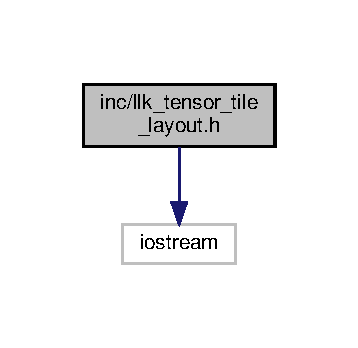
\includegraphics[width=172pt]{llk__tensor__tile__layout_8h__incl}
\end{center}
\end{figure}
This graph shows which files directly or indirectly include this file\+:\nopagebreak
\begin{figure}[H]
\begin{center}
\leavevmode
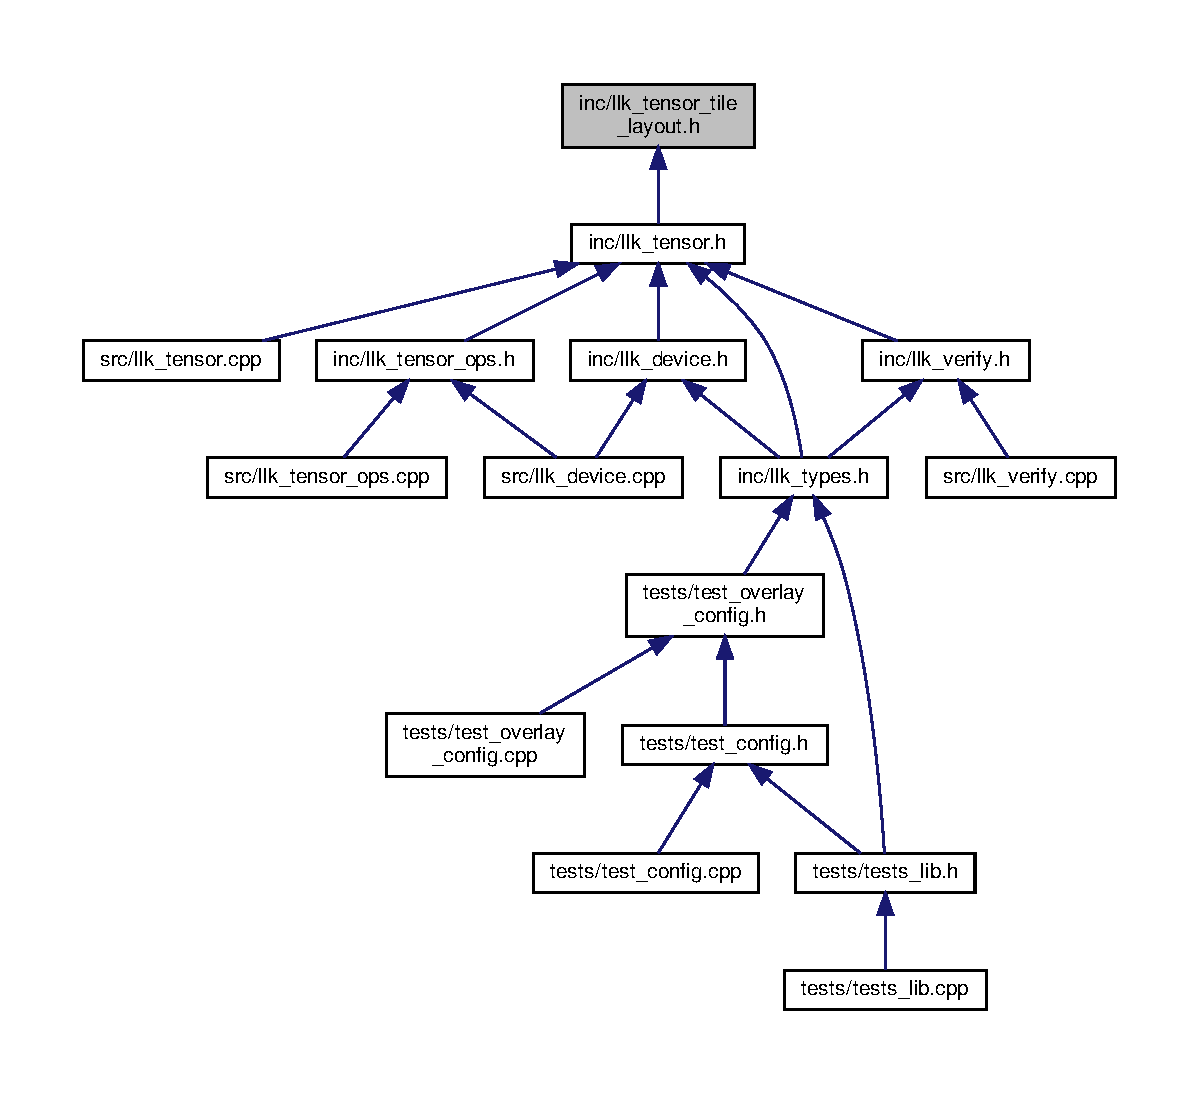
\includegraphics[width=350pt]{llk__tensor__tile__layout_8h__dep__incl}
\end{center}
\end{figure}
\subsection*{Namespaces}
\begin{DoxyCompactItemize}
\item 
 \hyperlink{namespacellk}{llk}
\end{DoxyCompactItemize}
\subsection*{Enumerations}
\begin{DoxyCompactItemize}
\item 
enum \hyperlink{namespacellk_a1cb439631a4f96e1431eea4d9b1f5cdb}{llk\+::\+Tensor\+Tile\+Layout} \{ \hyperlink{namespacellk_a1cb439631a4f96e1431eea4d9b1f5cdba2e0e3da7320c14734283fa14f8325ccc}{llk\+::\+C\+O\+L\+\_\+\+M\+A\+J\+OR}, 
\hyperlink{namespacellk_a1cb439631a4f96e1431eea4d9b1f5cdbae821cdf54f59066eb3b7eec07d767162}{llk\+::\+C\+O\+L\+\_\+\+M\+A\+J\+O\+R\+\_\+\+Z\+I\+G\+Z\+AG}, 
\hyperlink{namespacellk_a1cb439631a4f96e1431eea4d9b1f5cdba6c2bb79839cbccc8c0df9becfb00d8f8}{llk\+::\+R\+O\+W\+\_\+\+M\+A\+J\+OR}, 
\hyperlink{namespacellk_a1cb439631a4f96e1431eea4d9b1f5cdba48f4ef1c077ea476eeef659e85904170}{llk\+::\+R\+O\+W\+\_\+\+M\+A\+J\+O\+R\+\_\+\+Z\+I\+G\+Z\+AG}
 \}
\end{DoxyCompactItemize}

\hypertarget{llk__types_8h}{}\section{inc/llk\+\_\+types.h File Reference}
\label{llk__types_8h}\index{inc/llk\+\_\+types.\+h@{inc/llk\+\_\+types.\+h}}
{\ttfamily \#include \char`\"{}llk\+\_\+addresses.\+h\char`\"{}}\newline
{\ttfamily \#include \char`\"{}llk\+\_\+device.\+h\char`\"{}}\newline
{\ttfamily \#include \char`\"{}llk\+\_\+hexfile.\+h\char`\"{}}\newline
{\ttfamily \#include \char`\"{}llk\+\_\+memory.\+h\char`\"{}}\newline
{\ttfamily \#include \char`\"{}llk\+\_\+soc\+\_\+descriptor.\+h\char`\"{}}\newline
{\ttfamily \#include \char`\"{}llk\+\_\+tensor.\+h\char`\"{}}\newline
{\ttfamily \#include \char`\"{}llk\+\_\+verify.\+h\char`\"{}}\newline
{\ttfamily \#include \char`\"{}llk\+\_\+xy\+\_\+pair.\+h\char`\"{}}\newline
Include dependency graph for llk\+\_\+types.\+h\+:\nopagebreak
\begin{figure}[H]
\begin{center}
\leavevmode
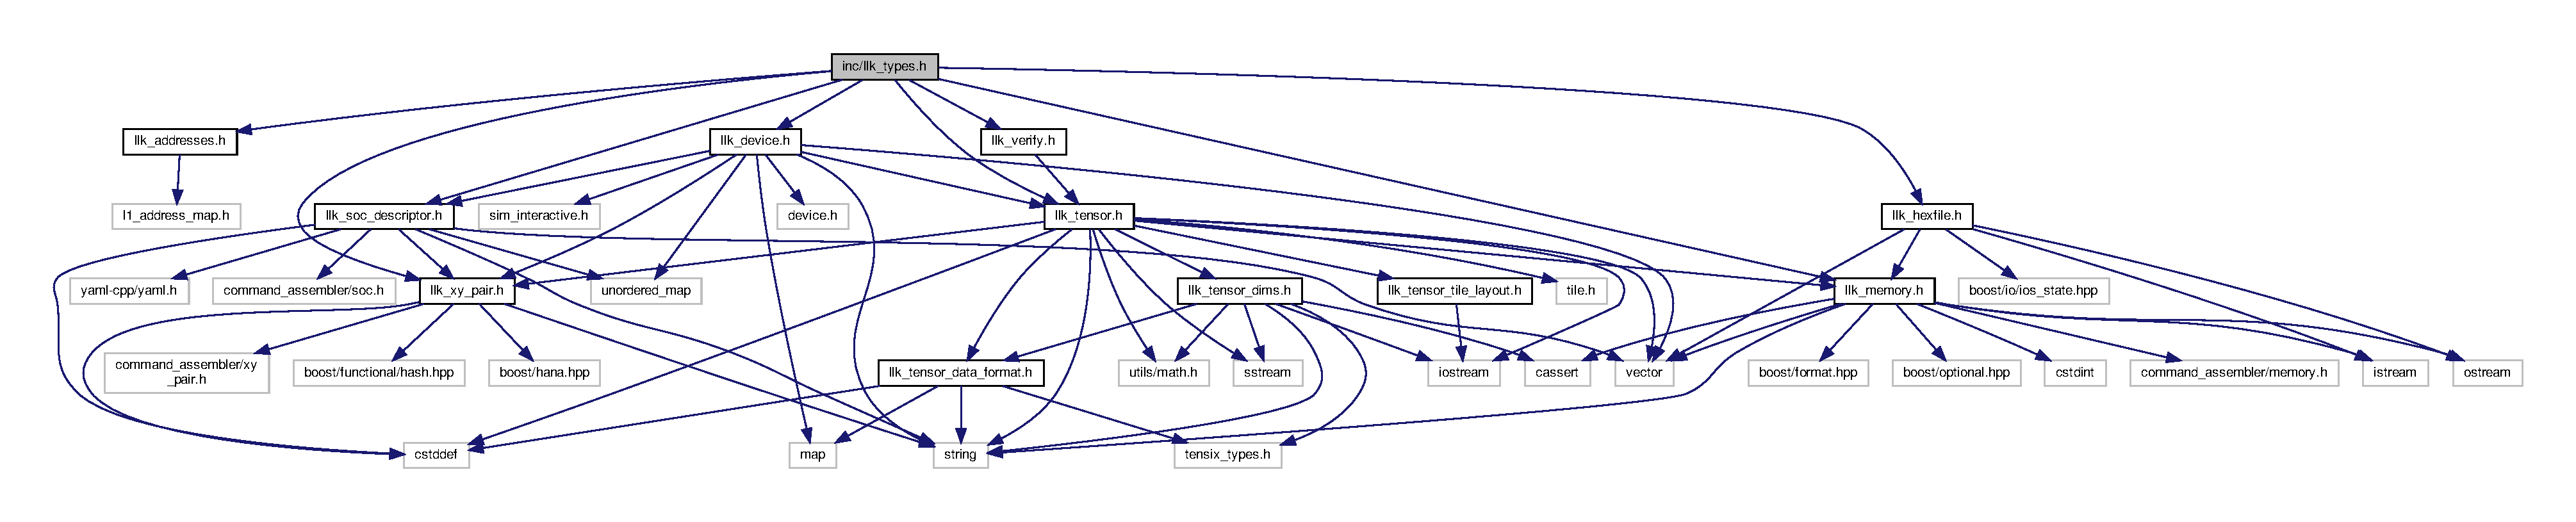
\includegraphics[width=350pt]{llk__types_8h__incl}
\end{center}
\end{figure}
This graph shows which files directly or indirectly include this file\+:\nopagebreak
\begin{figure}[H]
\begin{center}
\leavevmode
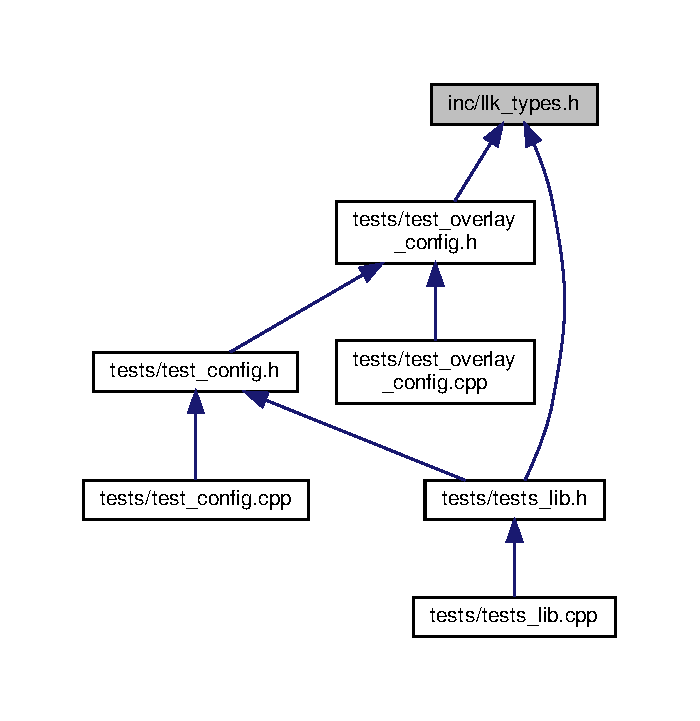
\includegraphics[width=336pt]{llk__types_8h__dep__incl}
\end{center}
\end{figure}

\hypertarget{llk__verify_8h}{}\section{inc/llk\+\_\+verify.h File Reference}
\label{llk__verify_8h}\index{inc/llk\+\_\+verify.\+h@{inc/llk\+\_\+verify.\+h}}
{\ttfamily \#include \char`\"{}llk\+\_\+tensor.\+h\char`\"{}}\newline
Include dependency graph for llk\+\_\+verify.\+h\+:\nopagebreak
\begin{figure}[H]
\begin{center}
\leavevmode
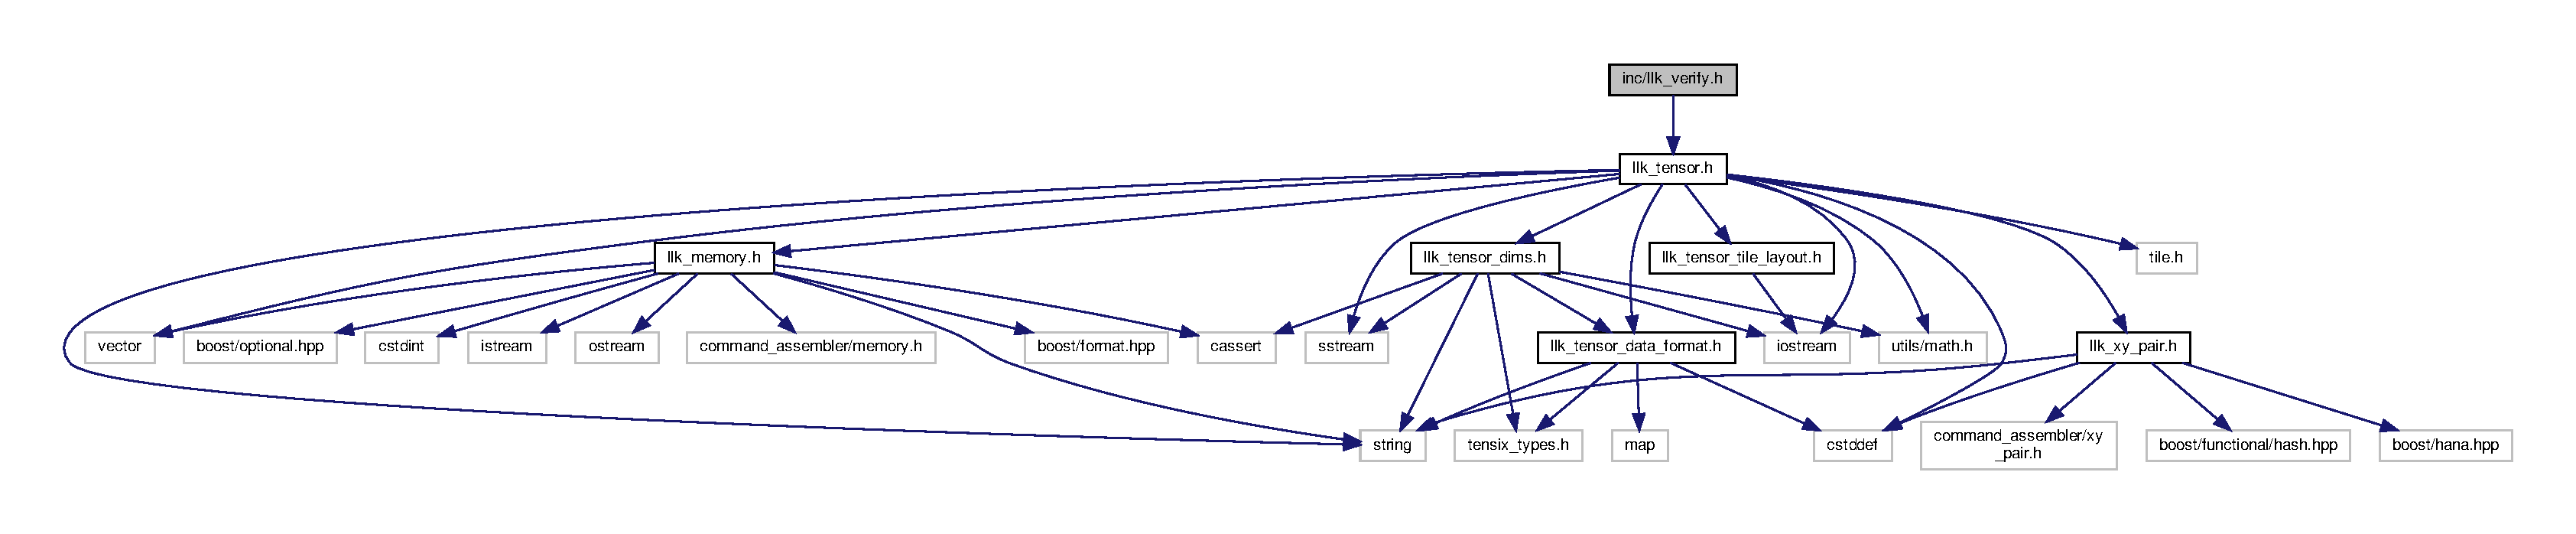
\includegraphics[width=350pt]{llk__verify_8h__incl}
\end{center}
\end{figure}
This graph shows which files directly or indirectly include this file\+:\nopagebreak
\begin{figure}[H]
\begin{center}
\leavevmode
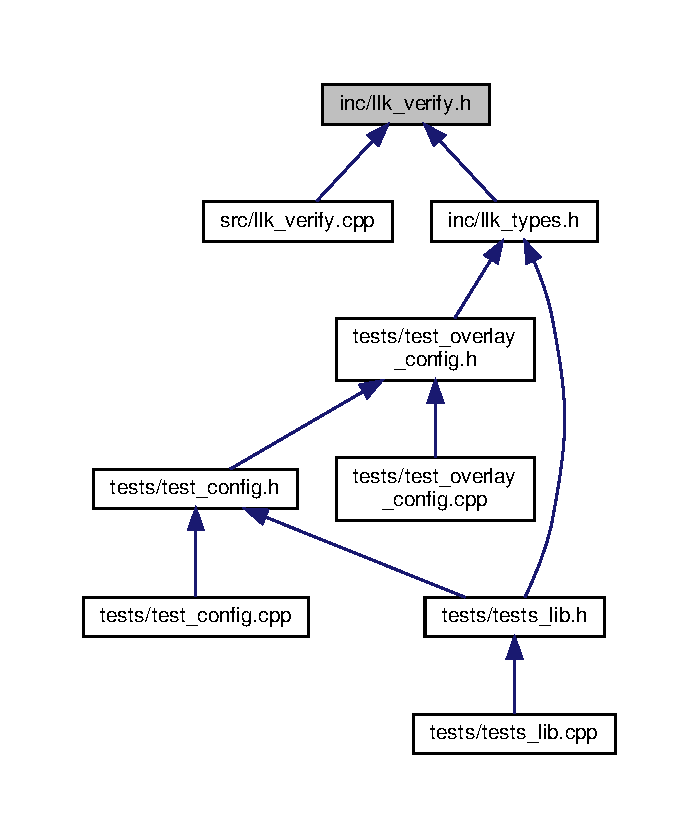
\includegraphics[width=336pt]{llk__verify_8h__dep__incl}
\end{center}
\end{figure}
\subsection*{Namespaces}
\begin{DoxyCompactItemize}
\item 
 \hyperlink{namespacellk}{llk}
\item 
 \hyperlink{namespacellk_1_1test__lib}{llk\+::test\+\_\+lib}
\begin{DoxyCompactList}\small\item\em \hyperlink{namespacellk_1_1test__lib}{test\+\_\+lib} is the exposed library functions to interface and interact with tests \end{DoxyCompactList}\end{DoxyCompactItemize}
\subsection*{Functions}
\begin{DoxyCompactItemize}
\item 
bool \hyperlink{namespacellk_a4177b29d9834c7885389009539d644d5}{llk\+::verify} (\hyperlink{classllk_1_1Tensor}{llk\+::\+Tensor} expected, \hyperlink{classllk_1_1Tensor}{llk\+::\+Tensor} calculated)
\end{DoxyCompactItemize}

\hypertarget{llk__xy__pair_8h}{}\section{inc/llk\+\_\+xy\+\_\+pair.h File Reference}
\label{llk__xy__pair_8h}\index{inc/llk\+\_\+xy\+\_\+pair.\+h@{inc/llk\+\_\+xy\+\_\+pair.\+h}}
{\ttfamily \#include $<$command\+\_\+assembler/xy\+\_\+pair.\+h$>$}\newline
{\ttfamily \#include $<$boost/functional/hash.\+hpp$>$}\newline
{\ttfamily \#include $<$boost/hana.\+hpp$>$}\newline
{\ttfamily \#include $<$cstddef$>$}\newline
{\ttfamily \#include $<$string$>$}\newline
Include dependency graph for llk\+\_\+xy\+\_\+pair.\+h\+:\nopagebreak
\begin{figure}[H]
\begin{center}
\leavevmode
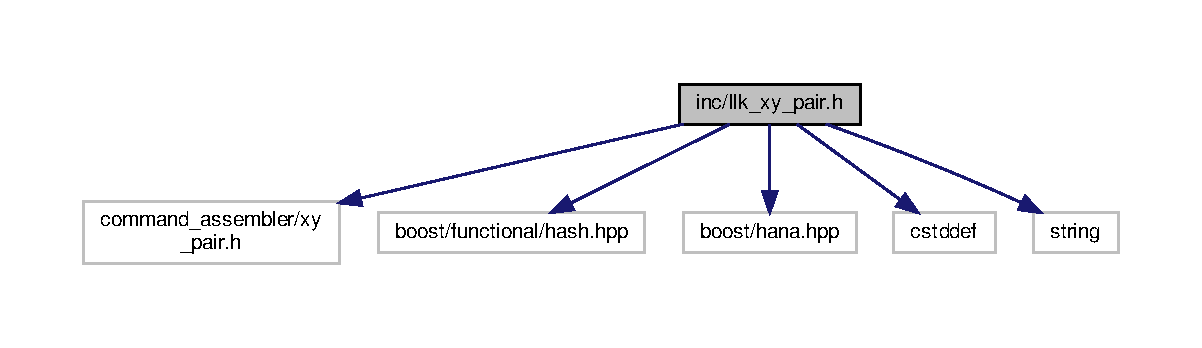
\includegraphics[width=350pt]{llk__xy__pair_8h__incl}
\end{center}
\end{figure}
This graph shows which files directly or indirectly include this file\+:\nopagebreak
\begin{figure}[H]
\begin{center}
\leavevmode
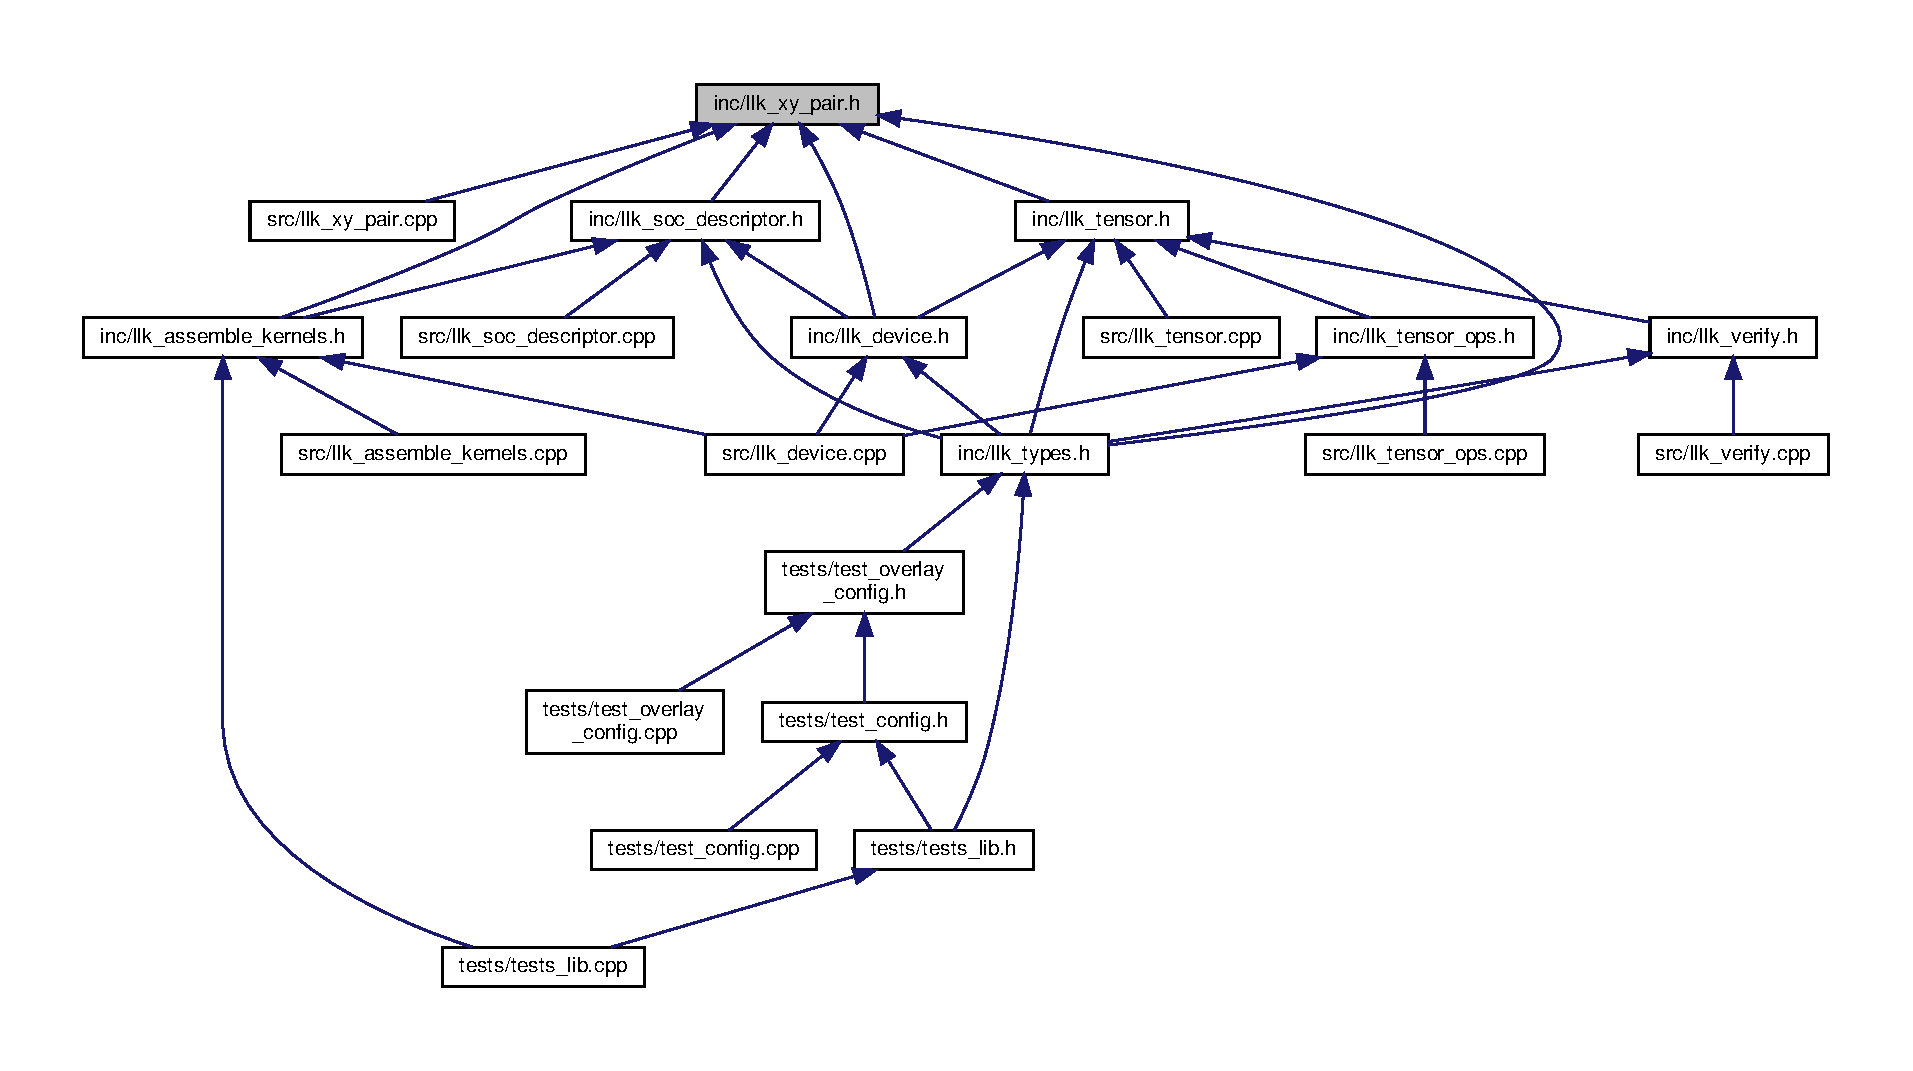
\includegraphics[width=350pt]{llk__xy__pair_8h__dep__incl}
\end{center}
\end{figure}
\subsection*{Classes}
\begin{DoxyCompactItemize}
\item 
struct \hyperlink{structllk_1_1xy__pair}{llk\+::xy\+\_\+pair}
\item 
struct \hyperlink{structstd_1_1hash_3_01llk_1_1xy__pair_01_4}{std\+::hash$<$ llk\+::xy\+\_\+pair $>$}
\end{DoxyCompactItemize}
\subsection*{Namespaces}
\begin{DoxyCompactItemize}
\item 
 \hyperlink{namespacellk}{llk}
\item 
 \hyperlink{namespacestd}{std}
\end{DoxyCompactItemize}
\subsection*{Functions}
\begin{DoxyCompactItemize}
\item 
constexpr bool \hyperlink{namespacellk_af1f5667d80a5b9802c82d0b618ae6c84}{llk\+::operator==} (const xy\+\_\+pair \&a, const xy\+\_\+pair \&b)
\item 
constexpr bool \hyperlink{namespacellk_a9bf058100a0317833cd763f8f2e74fbf}{llk\+::operator!=} (const xy\+\_\+pair \&a, const xy\+\_\+pair \&b)
\item 
constexpr bool \hyperlink{namespacellk_a23565b6066cff81531570244007bdbd3}{llk\+::operator$<$} (const xy\+\_\+pair \&left, const xy\+\_\+pair \&right)
\item 
std\+::string \hyperlink{namespacellk_acc9374b9eb2016cc65e6efd3300a9480}{llk\+::format\+\_\+node} (\hyperlink{structllk_1_1xy__pair}{xy\+\_\+pair} xy)
\item 
\hyperlink{structllk_1_1xy__pair}{xy\+\_\+pair} \hyperlink{namespacellk_aa3ef0c59d3d30e3643a2bab665aa164c}{llk\+::format\+\_\+node} (std\+::string str)
\end{DoxyCompactItemize}

\hypertarget{llk__assemble__kernels_8cpp}{}\section{src/llk\+\_\+assemble\+\_\+kernels.cpp File Reference}
\label{llk__assemble__kernels_8cpp}\index{src/llk\+\_\+assemble\+\_\+kernels.\+cpp@{src/llk\+\_\+assemble\+\_\+kernels.\+cpp}}
{\ttfamily \#include \char`\"{}llk\+\_\+assemble\+\_\+kernels.\+h\char`\"{}}\newline
{\ttfamily \#include $<$glog/logging.\+h$>$}\newline
{\ttfamily \#include $<$llk\+\_\+addresses.\+h$>$}\newline
{\ttfamily \#include $<$cstddef$>$}\newline
{\ttfamily \#include $<$experimental/filesystem$>$}\newline
{\ttfamily \#include $<$fstream$>$}\newline
{\ttfamily \#include $<$iostream$>$}\newline
{\ttfamily \#include $<$mutex$>$}\newline
{\ttfamily \#include $<$sstream$>$}\newline
{\ttfamily \#include \char`\"{}stdlib.\+h\char`\"{}}\newline
Include dependency graph for llk\+\_\+assemble\+\_\+kernels.\+cpp\+:\nopagebreak
\begin{figure}[H]
\begin{center}
\leavevmode
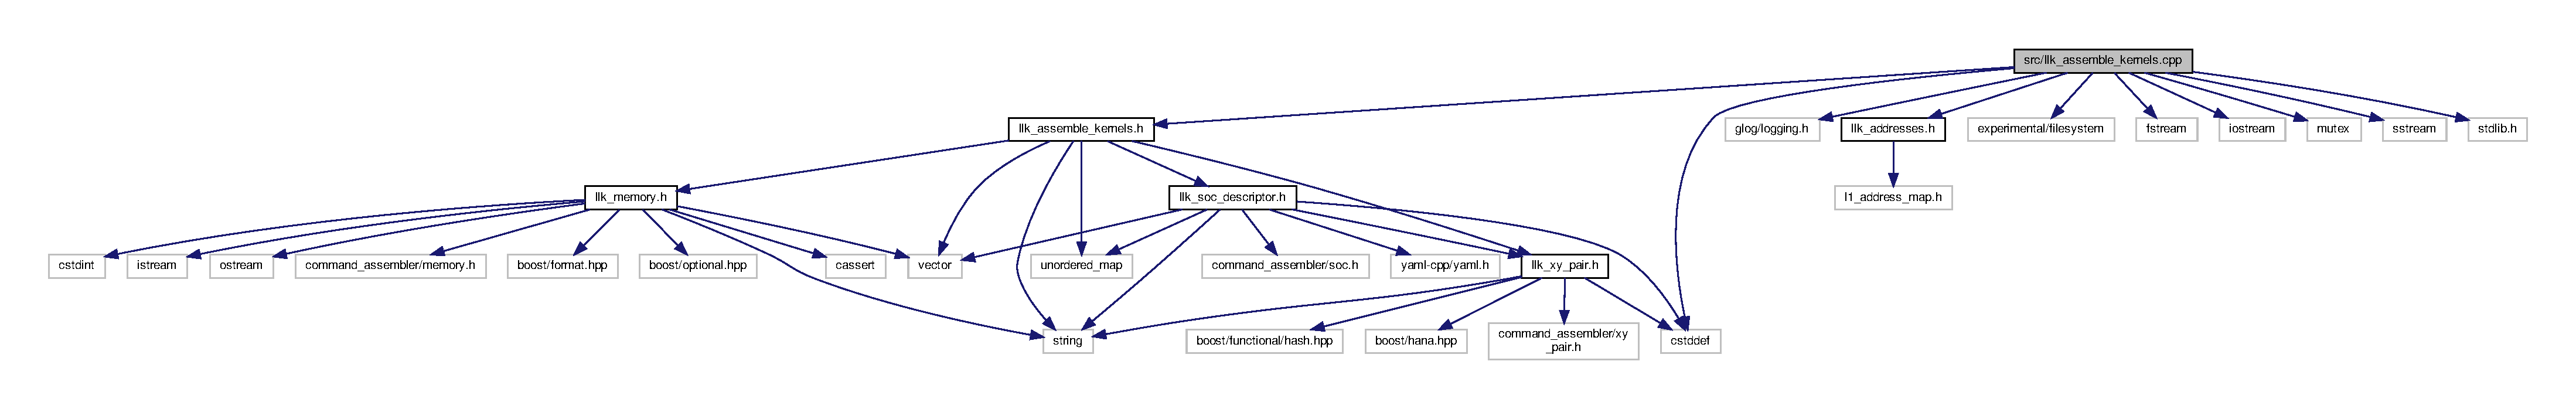
\includegraphics[width=350pt]{llk__assemble__kernels_8cpp__incl}
\end{center}
\end{figure}

\hypertarget{llk__device_8cpp}{}\section{src/llk\+\_\+device.cpp File Reference}
\label{llk__device_8cpp}\index{src/llk\+\_\+device.\+cpp@{src/llk\+\_\+device.\+cpp}}
{\ttfamily \#include \char`\"{}llk\+\_\+device.\+h\char`\"{}}\newline
{\ttfamily \#include $<$glog/logging.\+h$>$}\newline
{\ttfamily \#include $<$stdlib.\+h$>$}\newline
{\ttfamily \#include $<$unistd.\+h$>$}\newline
{\ttfamily \#include $<$chrono$>$}\newline
{\ttfamily \#include $<$cstddef$>$}\newline
{\ttfamily \#include $<$fstream$>$}\newline
{\ttfamily \#include $<$thread$>$}\newline
{\ttfamily \#include \char`\"{}llk\+\_\+addresses.\+h\char`\"{}}\newline
{\ttfamily \#include \char`\"{}llk\+\_\+assemble\+\_\+kernels.\+h\char`\"{}}\newline
{\ttfamily \#include \char`\"{}llk\+\_\+tensor\+\_\+ops.\+h\char`\"{}}\newline
Include dependency graph for llk\+\_\+device.\+cpp\+:\nopagebreak
\begin{figure}[H]
\begin{center}
\leavevmode
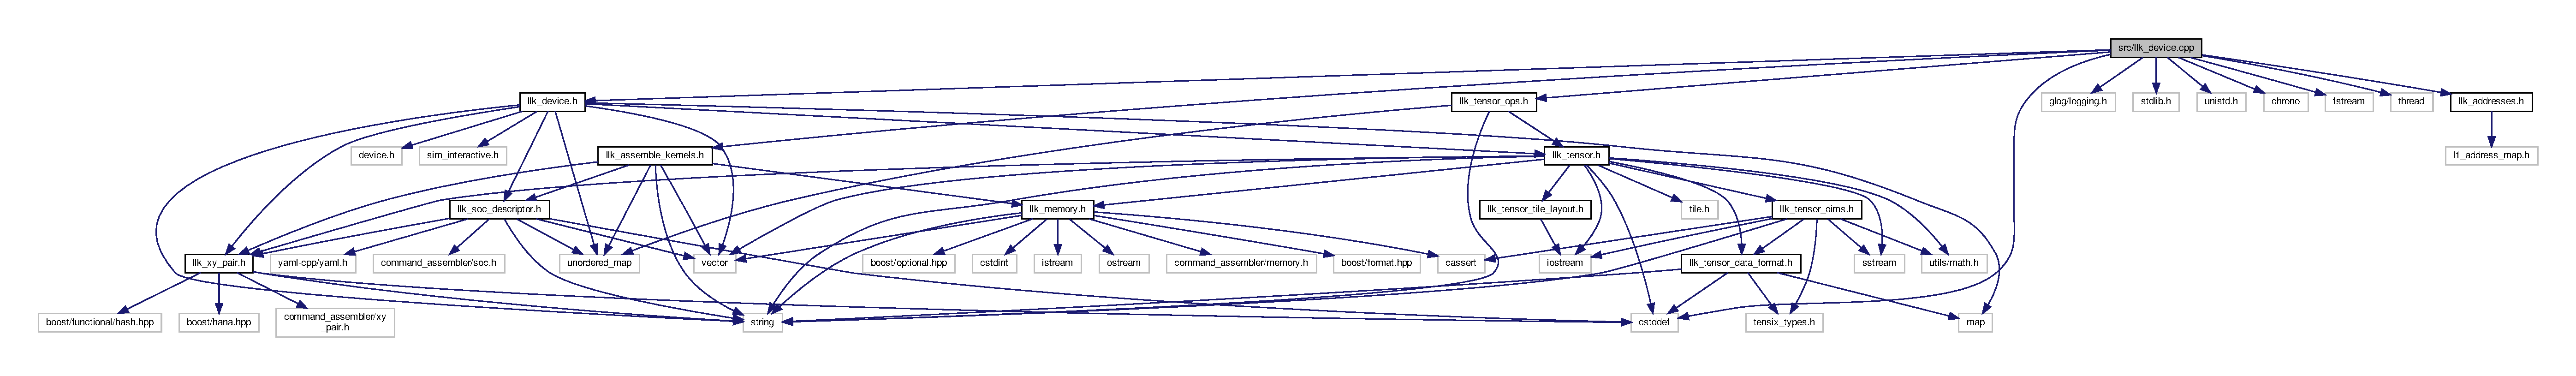
\includegraphics[width=350pt]{llk__device_8cpp__incl}
\end{center}
\end{figure}

\hypertarget{llk__hexfile_8cpp}{}\section{src/llk\+\_\+hexfile.cpp File Reference}
\label{llk__hexfile_8cpp}\index{src/llk\+\_\+hexfile.\+cpp@{src/llk\+\_\+hexfile.\+cpp}}
{\ttfamily \#include \char`\"{}llk\+\_\+hexfile.\+h\char`\"{}}\newline
{\ttfamily \#include $<$boost/spirit/include/qi.\+hpp$>$}\newline
{\ttfamily \#include $<$cassert$>$}\newline
{\ttfamily \#include $<$iomanip$>$}\newline
{\ttfamily \#include $<$limits$>$}\newline
{\ttfamily \#include $<$regex$>$}\newline
{\ttfamily \#include $<$stdexcept$>$}\newline
{\ttfamily \#include $<$string$>$}\newline
{\ttfamily \#include \char`\"{}llk\+\_\+rounding.\+h\char`\"{}}\newline
Include dependency graph for llk\+\_\+hexfile.\+cpp\+:\nopagebreak
\begin{figure}[H]
\begin{center}
\leavevmode
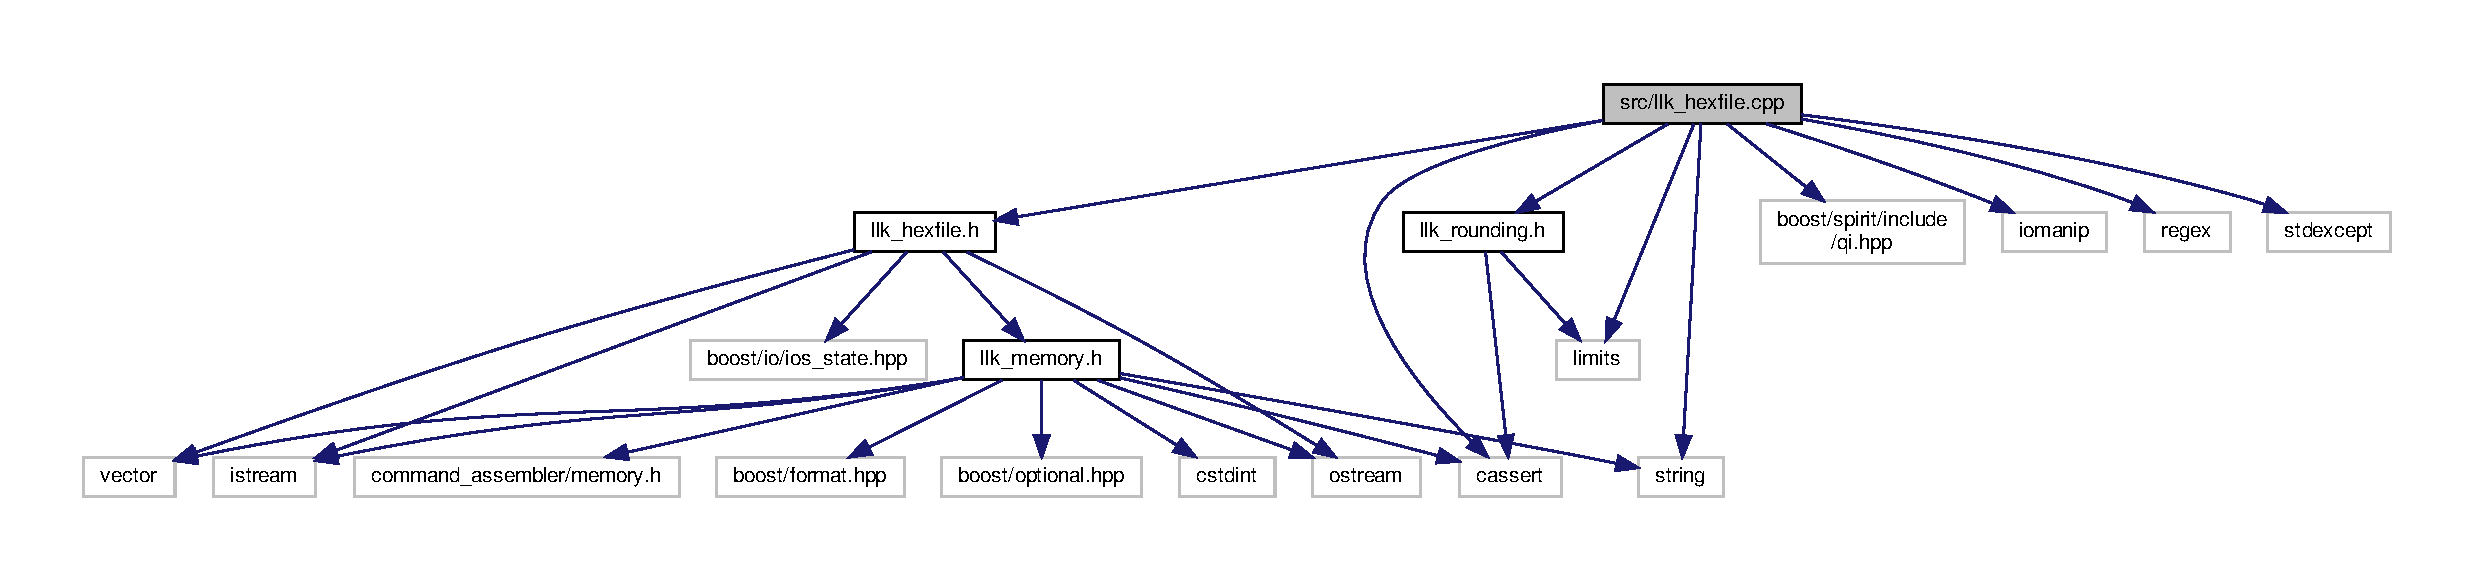
\includegraphics[width=350pt]{llk__hexfile_8cpp__incl}
\end{center}
\end{figure}
\subsection*{Namespaces}
\begin{DoxyCompactItemize}
\item 
 \hyperlink{namespacellk}{llk}
\end{DoxyCompactItemize}
\subsection*{Functions}
\begin{DoxyCompactItemize}
\item 
std\+::vector$<$ \hyperlink{classllk_1_1memory_a432a6c0ae1bcb9c44d79cfa1a239419c}{memory\+::word\+\_\+t} $>$ \hyperlink{namespacellk_abab62bc3369d43352be7b3f6b24a2717}{llk\+::read\+\_\+contiguous\+\_\+hex\+\_\+file} (std\+::istream \&input)
\item 
\hyperlink{classllk_1_1memory_ae7a4b897aa999f22e250dc8e4d773dec}{memory\+::address\+\_\+t} \hyperlink{namespacellk_a990d22b32661648e11a518ee5ce97f59}{llk\+::read\+\_\+contiguous\+\_\+hex\+\_\+file} (std\+::istream \&input, const std\+::function$<$ void(\hyperlink{classllk_1_1memory_ae7a4b897aa999f22e250dc8e4d773dec}{memory\+::address\+\_\+t}, \hyperlink{classllk_1_1memory_a432a6c0ae1bcb9c44d79cfa1a239419c}{memory\+::word\+\_\+t})$>$ \&callback, \hyperlink{classllk_1_1memory_ae7a4b897aa999f22e250dc8e4d773dec}{memory\+::address\+\_\+t} base)
\item 
\hyperlink{classllk_1_1memory_ae7a4b897aa999f22e250dc8e4d773dec}{memory\+::address\+\_\+t} \hyperlink{namespacellk_a8727be2796e20502d8401b0bd7090a31}{llk\+::read\+\_\+discontiguous\+\_\+hex\+\_\+file} (std\+::istream \&input, const std\+::function$<$ void(\hyperlink{classllk_1_1memory_ae7a4b897aa999f22e250dc8e4d773dec}{memory\+::address\+\_\+t}, \hyperlink{classllk_1_1memory_a432a6c0ae1bcb9c44d79cfa1a239419c}{memory\+::word\+\_\+t})$>$ \&callback)
\end{DoxyCompactItemize}

\hypertarget{llk__memory_8cpp}{}\section{src/llk\+\_\+memory.cpp File Reference}
\label{llk__memory_8cpp}\index{src/llk\+\_\+memory.\+cpp@{src/llk\+\_\+memory.\+cpp}}
{\ttfamily \#include \char`\"{}llk\+\_\+memory.\+h\char`\"{}}\newline
{\ttfamily \#include $<$cassert$>$}\newline
{\ttfamily \#include $<$cstdio$>$}\newline
{\ttfamily \#include $<$fstream$>$}\newline
{\ttfamily \#include $<$limits$>$}\newline
{\ttfamily \#include $<$stdexcept$>$}\newline
{\ttfamily \#include \char`\"{}llk\+\_\+hexfile.\+h\char`\"{}}\newline
Include dependency graph for llk\+\_\+memory.\+cpp\+:\nopagebreak
\begin{figure}[H]
\begin{center}
\leavevmode
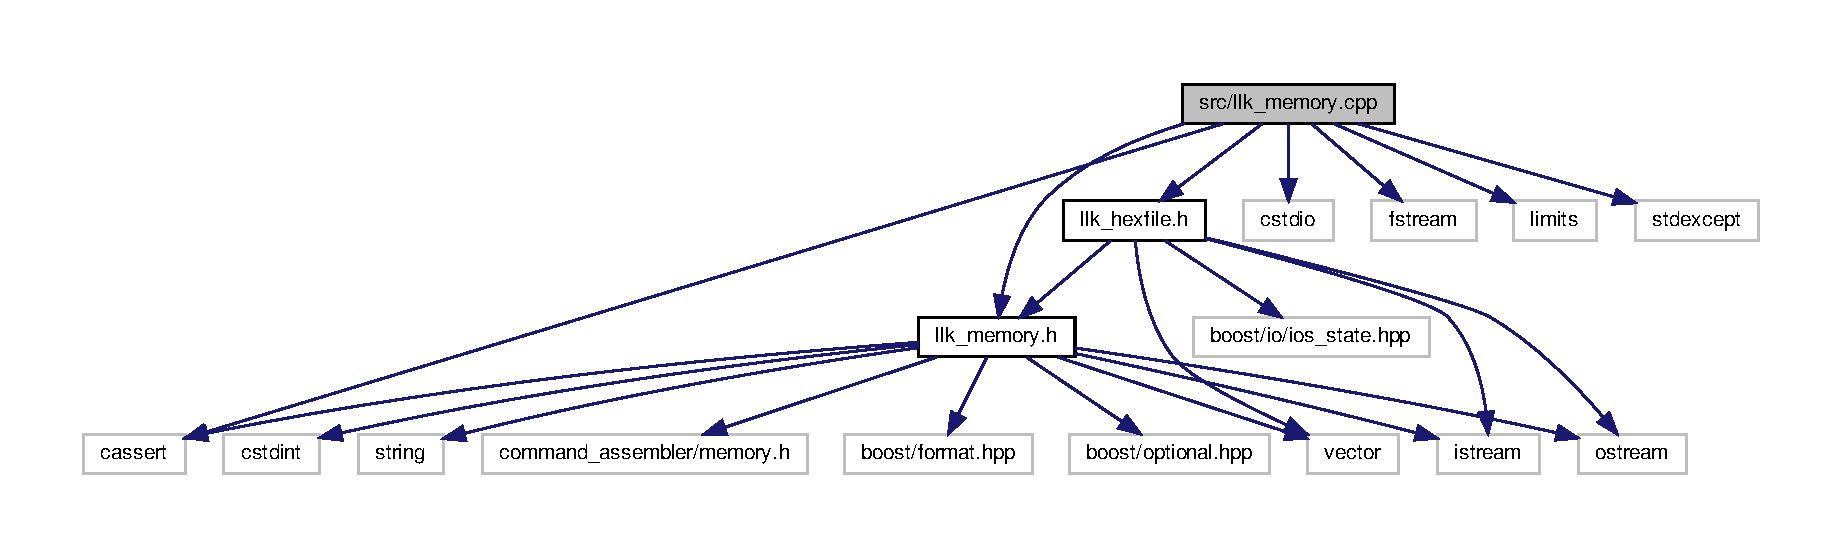
\includegraphics[width=350pt]{llk__memory_8cpp__incl}
\end{center}
\end{figure}
\subsection*{Namespaces}
\begin{DoxyCompactItemize}
\item 
 \hyperlink{namespacellk}{llk}
\end{DoxyCompactItemize}
\subsection*{Functions}
\begin{DoxyCompactItemize}
\item 
memory \hyperlink{namespacellk_adb43fe0eeac466803ff0566f52b4f7a8}{llk\+::slice\+\_\+memory} (const memory \&mem, memory\+::address\+\_\+t base, memory\+::address\+\_\+t start, memory\+::address\+\_\+t end)
\end{DoxyCompactItemize}

\hypertarget{llk__soc__descriptor_8cpp}{}\section{src/llk\+\_\+soc\+\_\+descriptor.cpp File Reference}
\label{llk__soc__descriptor_8cpp}\index{src/llk\+\_\+soc\+\_\+descriptor.\+cpp@{src/llk\+\_\+soc\+\_\+descriptor.\+cpp}}
{\ttfamily \#include \char`\"{}llk\+\_\+soc\+\_\+descriptor.\+h\char`\"{}}\newline
{\ttfamily \#include $<$boost/algorithm/string.\+hpp$>$}\newline
{\ttfamily \#include $<$boost/filesystem.\+hpp$>$}\newline
{\ttfamily \#include \char`\"{}glog/logging.\+h\char`\"{}}\newline
{\ttfamily \#include \char`\"{}llk\+\_\+addresses.\+h\char`\"{}}\newline
Include dependency graph for llk\+\_\+soc\+\_\+descriptor.\+cpp\+:\nopagebreak
\begin{figure}[H]
\begin{center}
\leavevmode
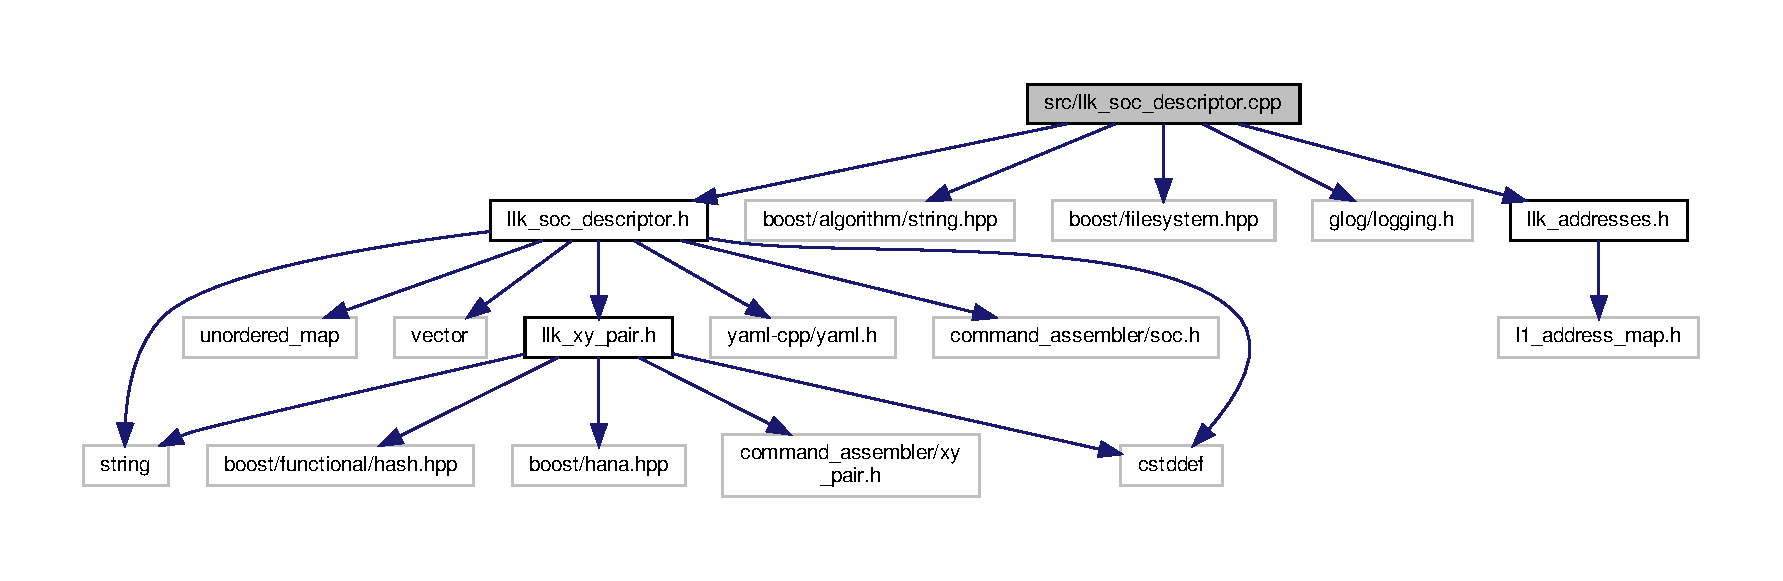
\includegraphics[width=350pt]{llk__soc__descriptor_8cpp__incl}
\end{center}
\end{figure}

\hypertarget{llk__tensor_8cpp}{}\section{src/llk\+\_\+tensor.cpp File Reference}
\label{llk__tensor_8cpp}\index{src/llk\+\_\+tensor.\+cpp@{src/llk\+\_\+tensor.\+cpp}}
{\ttfamily \#include \char`\"{}llk\+\_\+tensor.\+h\char`\"{}}\newline
{\ttfamily \#include $<$boost/filesystem.\+hpp$>$}\newline
{\ttfamily \#include $<$cassert$>$}\newline
{\ttfamily \#include $<$random$>$}\newline
{\ttfamily \#include $<$string$>$}\newline
{\ttfamily \#include $<$unordered\+\_\+map$>$}\newline
{\ttfamily \#include \char`\"{}glog/logging.\+h\char`\"{}}\newline
{\ttfamily \#include \char`\"{}utils/distributions.\+h\char`\"{}}\newline
Include dependency graph for llk\+\_\+tensor.\+cpp\+:\nopagebreak
\begin{figure}[H]
\begin{center}
\leavevmode
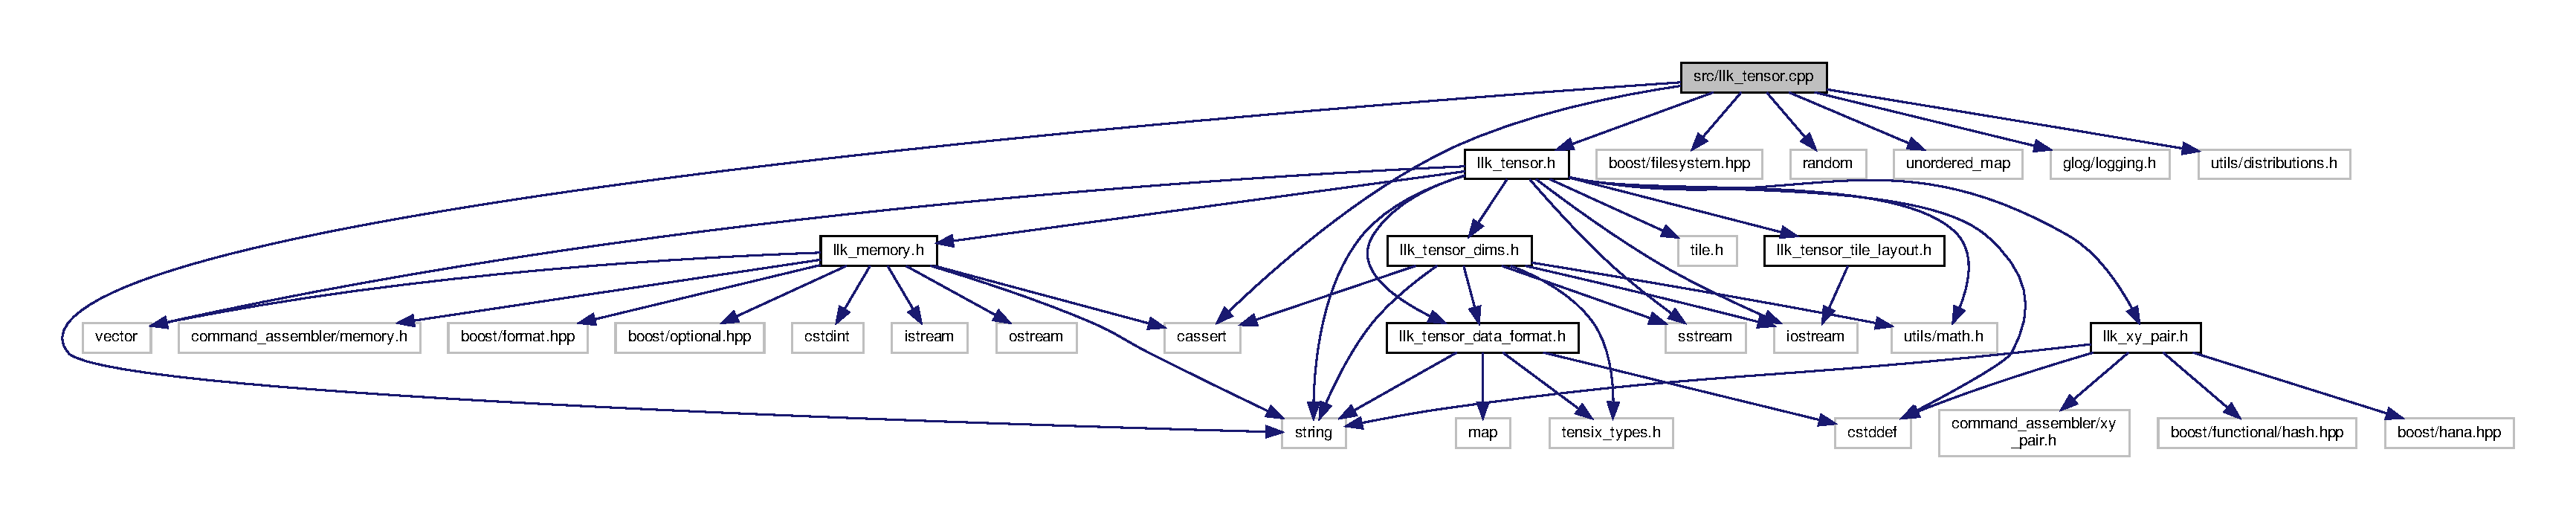
\includegraphics[width=350pt]{llk__tensor_8cpp__incl}
\end{center}
\end{figure}

\hypertarget{llk__tensor__data__format_8cpp}{}\section{src/llk\+\_\+tensor\+\_\+data\+\_\+format.cpp File Reference}
\label{llk__tensor__data__format_8cpp}\index{src/llk\+\_\+tensor\+\_\+data\+\_\+format.\+cpp@{src/llk\+\_\+tensor\+\_\+data\+\_\+format.\+cpp}}
{\ttfamily \#include \char`\"{}llk\+\_\+tensor\+\_\+data\+\_\+format.\+h\char`\"{}}\newline
{\ttfamily \#include $<$iostream$>$}\newline
{\ttfamily \#include \char`\"{}tile.\+h\char`\"{}}\newline
Include dependency graph for llk\+\_\+tensor\+\_\+data\+\_\+format.\+cpp\+:\nopagebreak
\begin{figure}[H]
\begin{center}
\leavevmode
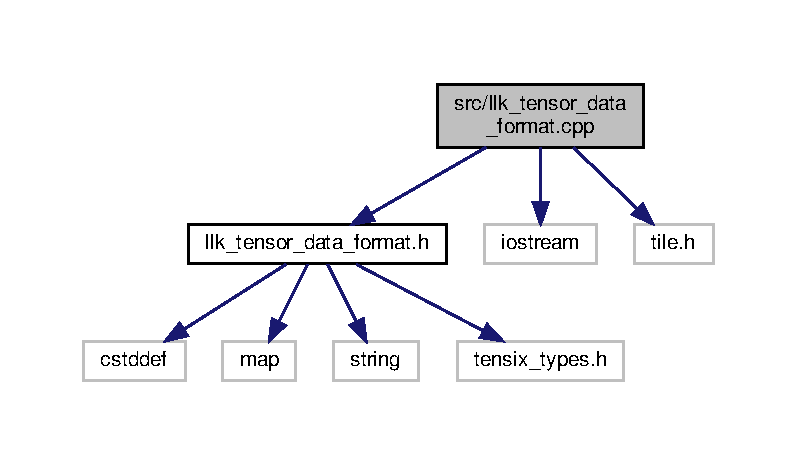
\includegraphics[width=350pt]{llk__tensor__data__format_8cpp__incl}
\end{center}
\end{figure}

\hypertarget{llk__tensor__ops_8cpp}{}\section{src/llk\+\_\+tensor\+\_\+ops.cpp File Reference}
\label{llk__tensor__ops_8cpp}\index{src/llk\+\_\+tensor\+\_\+ops.\+cpp@{src/llk\+\_\+tensor\+\_\+ops.\+cpp}}
{\ttfamily \#include \char`\"{}llk\+\_\+tensor\+\_\+ops.\+h\char`\"{}}\newline
{\ttfamily \#include \char`\"{}glog/logging.\+h\char`\"{}}\newline
{\ttfamily \#include \char`\"{}llk\+\_\+tensor\+\_\+dims.\+h\char`\"{}}\newline
Include dependency graph for llk\+\_\+tensor\+\_\+ops.\+cpp\+:\nopagebreak
\begin{figure}[H]
\begin{center}
\leavevmode
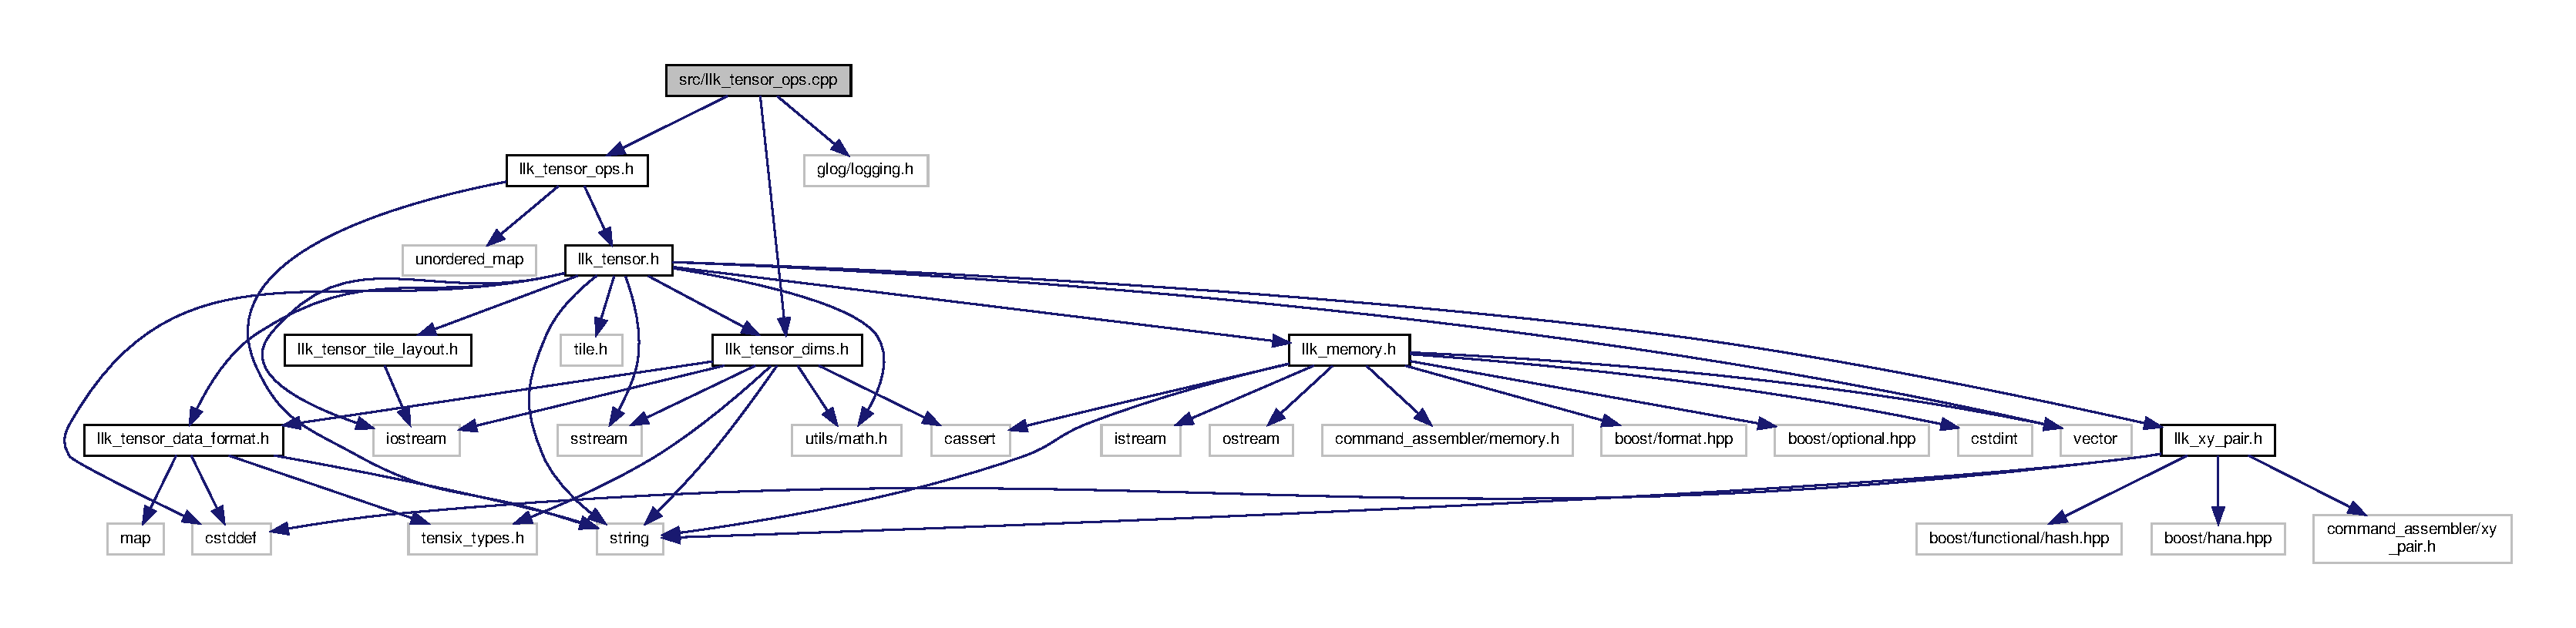
\includegraphics[width=350pt]{llk__tensor__ops_8cpp__incl}
\end{center}
\end{figure}

\hypertarget{llk__verify_8cpp}{}\section{src/llk\+\_\+verify.cpp File Reference}
\label{llk__verify_8cpp}\index{src/llk\+\_\+verify.\+cpp@{src/llk\+\_\+verify.\+cpp}}
{\ttfamily \#include \char`\"{}llk\+\_\+verify.\+h\char`\"{}}\newline
{\ttfamily \#include $<$glog/logging.\+h$>$}\newline
{\ttfamily \#include $<$unordered\+\_\+map$>$}\newline
Include dependency graph for llk\+\_\+verify.\+cpp\+:\nopagebreak
\begin{figure}[H]
\begin{center}
\leavevmode
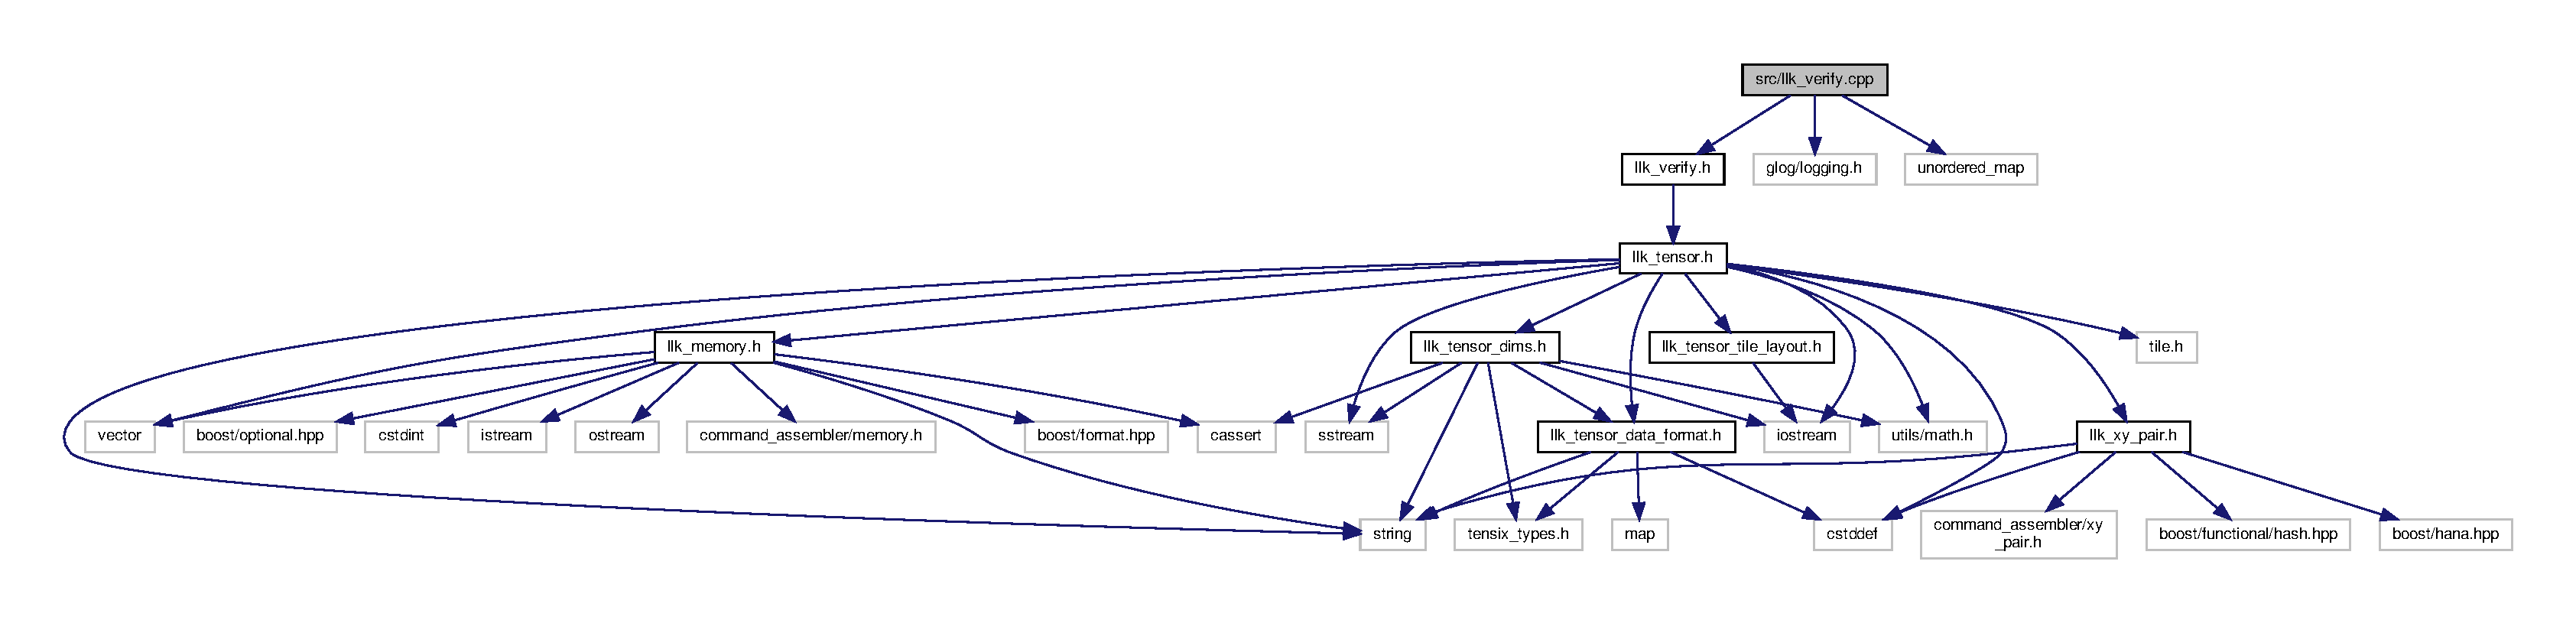
\includegraphics[width=350pt]{llk__verify_8cpp__incl}
\end{center}
\end{figure}

\hypertarget{llk__xy__pair_8cpp}{}\section{src/llk\+\_\+xy\+\_\+pair.cpp File Reference}
\label{llk__xy__pair_8cpp}\index{src/llk\+\_\+xy\+\_\+pair.\+cpp@{src/llk\+\_\+xy\+\_\+pair.\+cpp}}
{\ttfamily \#include \char`\"{}llk\+\_\+xy\+\_\+pair.\+h\char`\"{}}\newline
{\ttfamily \#include $<$regex$>$}\newline
{\ttfamily \#include $<$stdexcept$>$}\newline
{\ttfamily \#include $<$string$>$}\newline
Include dependency graph for llk\+\_\+xy\+\_\+pair.\+cpp\+:\nopagebreak
\begin{figure}[H]
\begin{center}
\leavevmode
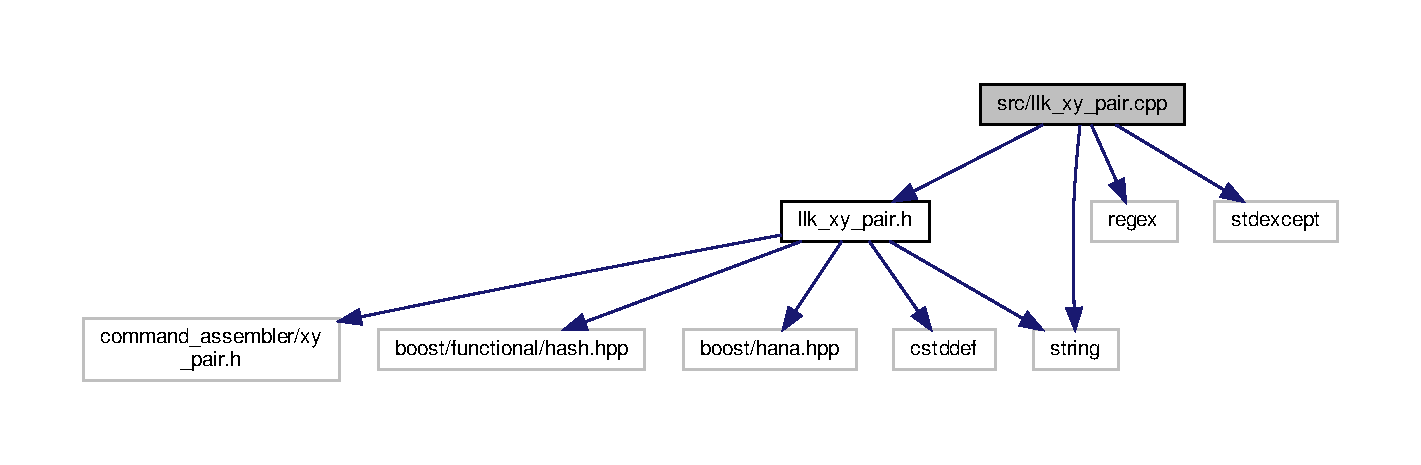
\includegraphics[width=350pt]{llk__xy__pair_8cpp__incl}
\end{center}
\end{figure}

\hypertarget{test__args_8h}{}\section{tests/test\+\_\+args.h File Reference}
\label{test__args_8h}\index{tests/test\+\_\+args.\+h@{tests/test\+\_\+args.\+h}}
{\ttfamily \#include $<$string$>$}\newline
{\ttfamily \#include $<$vector$>$}\newline
Include dependency graph for test\+\_\+args.\+h\+:\nopagebreak
\begin{figure}[H]
\begin{center}
\leavevmode
\includegraphics[width=184pt]{test__args_8h__incl}
\end{center}
\end{figure}
This graph shows which files directly or indirectly include this file\+:\nopagebreak
\begin{figure}[H]
\begin{center}
\leavevmode
\includegraphics[width=349pt]{test__args_8h__dep__incl}
\end{center}
\end{figure}
\subsection*{Classes}
\begin{DoxyCompactItemize}
\item 
struct \hyperlink{structtests_1_1TestArgs}{tests\+::\+Test\+Args}
\end{DoxyCompactItemize}
\subsection*{Namespaces}
\begin{DoxyCompactItemize}
\item 
 \hyperlink{namespacetests}{tests}
\end{DoxyCompactItemize}

\hypertarget{test__config_8cpp}{}\section{tests/test\+\_\+config.cpp File Reference}
\label{test__config_8cpp}\index{tests/test\+\_\+config.\+cpp@{tests/test\+\_\+config.\+cpp}}
{\ttfamily \#include \char`\"{}test\+\_\+config.\+h\char`\"{}}\newline
{\ttfamily \#include \char`\"{}experimental/filesystem\char`\"{}}\newline
Include dependency graph for test\+\_\+config.\+cpp\+:\nopagebreak
\begin{figure}[H]
\begin{center}
\leavevmode
\includegraphics[width=350pt]{test__config_8cpp__incl}
\end{center}
\end{figure}

\hypertarget{test__config_8h}{}\section{tests/test\+\_\+config.h File Reference}
\label{test__config_8h}\index{tests/test\+\_\+config.\+h@{tests/test\+\_\+config.\+h}}
{\ttfamily \#include $<$chrono$>$}\newline
{\ttfamily \#include $<$map$>$}\newline
{\ttfamily \#include $<$string$>$}\newline
{\ttfamily \#include \char`\"{}test\+\_\+args.\+h\char`\"{}}\newline
{\ttfamily \#include \char`\"{}test\+\_\+kernel\+\_\+params.\+h\char`\"{}}\newline
{\ttfamily \#include \char`\"{}test\+\_\+overlay\+\_\+config.\+h\char`\"{}}\newline
{\ttfamily \#include \char`\"{}test\+\_\+tensor\+\_\+config.\+h\char`\"{}}\newline
{\ttfamily \#include \char`\"{}yaml-\/cpp/yaml.\+h\char`\"{}}\newline
Include dependency graph for test\+\_\+config.\+h\+:\nopagebreak
\begin{figure}[H]
\begin{center}
\leavevmode
\includegraphics[width=350pt]{test__config_8h__incl}
\end{center}
\end{figure}
This graph shows which files directly or indirectly include this file\+:\nopagebreak
\begin{figure}[H]
\begin{center}
\leavevmode
\includegraphics[width=298pt]{test__config_8h__dep__incl}
\end{center}
\end{figure}
\subsection*{Classes}
\begin{DoxyCompactItemize}
\item 
struct \hyperlink{structtests_1_1SingleCoreTestConfig}{tests\+::\+Single\+Core\+Test\+Config}
\begin{DoxyCompactList}\small\item\em \hyperlink{structtests_1_1TestConfig}{Test\+Config} specification for a specific core. \end{DoxyCompactList}\item 
struct \hyperlink{structtests_1_1TestConfig}{tests\+::\+Test\+Config}
\begin{DoxyCompactList}\small\item\em \hyperlink{structtests_1_1TestConfig}{Test\+Config} -\/ Config Structure. \end{DoxyCompactList}\end{DoxyCompactItemize}
\subsection*{Namespaces}
\begin{DoxyCompactItemize}
\item 
 \hyperlink{namespacetests}{tests}
\item 
 \hyperlink{namespacetests_1_1test__config__api}{tests\+::test\+\_\+config\+\_\+api}
\end{DoxyCompactItemize}
\subsection*{Enumerations}
\begin{DoxyCompactItemize}
\item 
enum \hyperlink{namespacetests_a4f360b8af533762256ff97513bfd6a0d}{tests\+::\+Kernel\+Type} \{ \hyperlink{namespacetests_a4f360b8af533762256ff97513bfd6a0daba3bbf795bfdbe156772d8f44833a3af}{tests\+::\+U\+N\+P\+A\+CK}, 
\hyperlink{namespacetests_a4f360b8af533762256ff97513bfd6a0da7b849aa2899a63a2da359bf9a0b5b0af}{tests\+::\+M\+A\+TH}, 
\hyperlink{namespacetests_a4f360b8af533762256ff97513bfd6a0daa484d944b59301977fbe221d69d58857}{tests\+::\+P\+A\+CK}
 \}\begin{DoxyCompactList}\small\item\em Kernel\+Type is meant as a enumeration for the type of kernels supported in yaml/config. \end{DoxyCompactList}
\end{DoxyCompactItemize}
\subsection*{Functions}
\begin{DoxyCompactItemize}
\item 
Kernel\+Type \hyperlink{namespacetests_a6596994244a2884f6810ad1592c25c36}{tests\+::get\+\_\+kernel\+\_\+type\+\_\+from\+\_\+string} (string kernel\+\_\+type\+\_\+string)
\item 
string \hyperlink{namespacetests_ad75f85658266305d587bfb6795c1922e}{tests\+::get\+\_\+string\+\_\+from\+\_\+kernel\+\_\+type} (Kernel\+Type kernel\+\_\+type)
\item 
void \hyperlink{namespacetests_1_1test__config__api_a3c68a5d0f35112a785ff8dea44d7d1e7}{tests\+::test\+\_\+config\+\_\+api\+::read\+\_\+tensor\+\_\+config\+\_\+from\+\_\+yaml} (Test\+Config \&test\+\_\+config, Y\+A\+M\+L\+::\+Node \&test\+\_\+descriptor)
\begin{DoxyCompactList}\small\item\em Read test-\/config.\+tensor-\/config sections from a yaml. \end{DoxyCompactList}\item 
void \hyperlink{namespacetests_1_1test__config__api_a535396ca6d07ebe33c1232eda6bded29}{tests\+::test\+\_\+config\+\_\+api\+::read\+\_\+extra\+\_\+config\+\_\+from\+\_\+yaml} (Test\+Config \&test\+\_\+config, Y\+A\+M\+L\+::\+Node \&test\+\_\+descriptor)
\begin{DoxyCompactList}\small\item\em Read test-\/config.\+extra-\/config sections from a yaml. \end{DoxyCompactList}\item 
void \hyperlink{namespacetests_1_1test__config__api_a6c9809f23745f5da467bfbe2a866c4a8}{tests\+::test\+\_\+config\+\_\+api\+::read\+\_\+test\+\_\+config\+\_\+from\+\_\+yaml} (Test\+Config \&test\+\_\+config, Y\+A\+M\+L\+::\+Node \&test\+\_\+descriptor)
\begin{DoxyCompactList}\small\item\em Read the test-\/config section from a yaml. Top-\/level function to call if a yaml configuration needs to be pulled into the config. \end{DoxyCompactList}\item 
void \hyperlink{namespacetests_1_1test__config__api_a6907c47ab33d9fc64929313ace78cd37}{tests\+::test\+\_\+config\+\_\+api\+::update\+\_\+extra\+\_\+config} (Test\+Config \&test\+\_\+config, std\+::string key, std\+::string value)
\begin{DoxyCompactList}\small\item\em Add or set the extra config using \{key, value\} map. \end{DoxyCompactList}\item 
void \hyperlink{namespacetests_1_1test__config__api_afe5e56a2088573bf1a4ceabb01b2424d}{tests\+::test\+\_\+config\+\_\+api\+::update\+\_\+tensor\+\_\+config} (Test\+Config \&test\+\_\+config, string tensor\+\_\+name, \hyperlink{structtests_1_1TensorConfig}{tests\+::\+Tensor\+Config} \&tensor\+\_\+config)
\begin{DoxyCompactList}\small\item\em Update the tensor configration under the tensor name. Will overrite if it exists. \end{DoxyCompactList}\item 
void \hyperlink{namespacetests_1_1test__config__api_a06e47de4d6e6c2de865838ded3f52764}{tests\+::test\+\_\+config\+\_\+api\+::update\+\_\+tensor\+\_\+config} (Test\+Config \&test\+\_\+config, string tensor\+\_\+name, \hyperlink{structllk_1_1TensorDims}{llk\+::\+Tensor\+Dims} dim, Data\+Format data\+\_\+format)
\begin{DoxyCompactList}\small\item\em Update only the dimensions and data\+\_\+format for a specific tensor config. \end{DoxyCompactList}\item 
void \hyperlink{namespacetests_1_1test__config__api_acb29a0a49bb5ecb9cd6ca09eb6211ad1}{tests\+::test\+\_\+config\+\_\+api\+::clear\+\_\+kernel\+\_\+parameters} (Test\+Config \&test\+\_\+config, \hyperlink{structllk_1_1xy__pair}{llk\+::xy\+\_\+pair} coord, \hyperlink{namespacetests_a4f360b8af533762256ff97513bfd6a0d}{tests\+::\+Kernel\+Type} kernel\+\_\+type, std\+::string key, std\+::string value)
\begin{DoxyCompactList}\small\item\em Clear all kernel parameter mappings. \end{DoxyCompactList}\item 
void \hyperlink{namespacetests_1_1test__config__api_a056c9a76c1c2ac345492adad043a41f1}{tests\+::test\+\_\+config\+\_\+api\+::update\+\_\+kernel\+\_\+parameters} (Test\+Config \&test\+\_\+config, \hyperlink{structllk_1_1xy__pair}{llk\+::xy\+\_\+pair} coord, \hyperlink{namespacetests_a4f360b8af533762256ff97513bfd6a0d}{tests\+::\+Kernel\+Type} kernel\+\_\+type, std\+::string key, std\+::string value)
\begin{DoxyCompactList}\small\item\em Update Kernal parameters using \{key, value\} pair. Assign if it exists or create if it doesn\textquotesingle{}t. \end{DoxyCompactList}\item 
void \hyperlink{namespacetests_1_1test__config__api_aaedc4b39408b717d3868dbb7387bdc48}{tests\+::test\+\_\+config\+\_\+api\+::update\+\_\+kernel\+\_\+parameters} (Test\+Config \&test\+\_\+config, \hyperlink{structllk_1_1xy__pair}{llk\+::xy\+\_\+pair} coord, \hyperlink{namespacetests_a4f360b8af533762256ff97513bfd6a0d}{tests\+::\+Kernel\+Type} kernel\+\_\+type, std\+::map$<$ std\+::string, std\+::string $>$ param\+\_\+mappings)
\begin{DoxyCompactList}\small\item\em Update Kernal parameters using a map with \{key, value\} pairs. Assign all pairs to the kernel\+\_\+parameter mapping exists or create if it doesn\textquotesingle{}t. \end{DoxyCompactList}\item 
void \hyperlink{namespacetests_1_1test__config__api_a7c5f36113ab125d7740af42d52f9939c}{tests\+::test\+\_\+config\+\_\+api\+::update\+\_\+kernel\+\_\+parameters} (Test\+Config \&test\+\_\+config, \hyperlink{structllk_1_1xy__pair}{llk\+::xy\+\_\+pair} coord, \hyperlink{namespacetests_a4f360b8af533762256ff97513bfd6a0d}{tests\+::\+Kernel\+Type} kernel\+\_\+type, \hyperlink{structtests_1_1KernelParams}{tests\+::\+Kernel\+Params} kernel\+\_\+params)
\begin{DoxyCompactList}\small\item\em Override the specified kernel type\textquotesingle{}s kernel param mappings. \end{DoxyCompactList}\item 
void \hyperlink{namespacetests_1_1test__config__api_af3c341ace6617f546990ef3f49e55a24}{tests\+::test\+\_\+config\+\_\+api\+::update\+\_\+kernel\+\_\+used} (Test\+Config \&test\+\_\+config, \hyperlink{structllk_1_1xy__pair}{llk\+::xy\+\_\+pair} coord, \hyperlink{namespacetests_a4f360b8af533762256ff97513bfd6a0d}{tests\+::\+Kernel\+Type} kernel\+\_\+type, string base\+\_\+kernel\+\_\+name, string full\+\_\+kernel\+\_\+name)
\begin{DoxyCompactList}\small\item\em Override the kernel name used (Will need to provide the full name) \end{DoxyCompactList}\end{DoxyCompactItemize}

\hypertarget{test__kernel__params_8cpp}{}\section{tests/test\+\_\+kernel\+\_\+params.cpp File Reference}
\label{test__kernel__params_8cpp}\index{tests/test\+\_\+kernel\+\_\+params.\+cpp@{tests/test\+\_\+kernel\+\_\+params.\+cpp}}
{\ttfamily \#include \char`\"{}test\+\_\+kernel\+\_\+params.\+h\char`\"{}}\newline
{\ttfamily \#include $<$fstream$>$}\newline
{\ttfamily \#include $<$iostream$>$}\newline
Include dependency graph for test\+\_\+kernel\+\_\+params.\+cpp\+:\nopagebreak
\begin{figure}[H]
\begin{center}
\leavevmode
\includegraphics[width=330pt]{test__kernel__params_8cpp__incl}
\end{center}
\end{figure}

\hypertarget{test__kernel__params_8h}{}\section{tests/test\+\_\+kernel\+\_\+params.h File Reference}
\label{test__kernel__params_8h}\index{tests/test\+\_\+kernel\+\_\+params.\+h@{tests/test\+\_\+kernel\+\_\+params.\+h}}
{\ttfamily \#include $<$map$>$}\newline
{\ttfamily \#include $<$string$>$}\newline
Include dependency graph for test\+\_\+kernel\+\_\+params.\+h\+:\nopagebreak
\begin{figure}[H]
\begin{center}
\leavevmode
\includegraphics[width=215pt]{test__kernel__params_8h__incl}
\end{center}
\end{figure}
This graph shows which files directly or indirectly include this file\+:\nopagebreak
\begin{figure}[H]
\begin{center}
\leavevmode
\includegraphics[width=350pt]{test__kernel__params_8h__dep__incl}
\end{center}
\end{figure}
\subsection*{Classes}
\begin{DoxyCompactItemize}
\item 
struct \hyperlink{structtests_1_1KernelParams}{tests\+::\+Kernel\+Params}
\end{DoxyCompactItemize}
\subsection*{Namespaces}
\begin{DoxyCompactItemize}
\item 
 \hyperlink{namespacetests}{tests}
\end{DoxyCompactItemize}
\subsection*{Functions}
\begin{DoxyCompactItemize}
\item 
void \hyperlink{namespacetests_a669b08c547907fe0dcb3219b3b8142c7}{tests\+::clear\+\_\+param\+\_\+mapping} (Kernel\+Params \&kernel\+\_\+params)
\item 
void \hyperlink{namespacetests_ac5d7bfff1d97fa0a9d6e5f7694a88921}{tests\+::del\+\_\+param\+\_\+mapping} (Kernel\+Params \&kernel\+\_\+params, std\+::string key)
\item 
void \hyperlink{namespacetests_a3ea8820101481a77d967610403ccd49d}{tests\+::add\+\_\+param\+\_\+mapping} (Kernel\+Params \&kernel\+\_\+params, std\+::string key, std\+::string val)
\item 
void \hyperlink{namespacetests_afa125cd17bd8f15a205cfa001c0cc0d9}{tests\+::add\+\_\+param\+\_\+mapping} (Kernel\+Params \&kernel\+\_\+params, std\+::map$<$ std\+::string, std\+::string $>$ \&override\+\_\+params)
\item 
void \hyperlink{namespacetests_aba02a7b523ddea64948c65e3d8721ec9}{tests\+::debug} (Kernel\+Params \&kernel\+\_\+params)
\end{DoxyCompactItemize}

\hypertarget{test__list_8h}{}\section{tests/test\+\_\+list.h File Reference}
\label{test__list_8h}\index{tests/test\+\_\+list.\+h@{tests/test\+\_\+list.\+h}}
{\ttfamily \#include $<$exception$>$}\newline
{\ttfamily \#include $<$iostream$>$}\newline
{\ttfamily \#include $<$string$>$}\newline
{\ttfamily \#include $<$unordered\+\_\+map$>$}\newline
{\ttfamily \#include \char`\"{}eltwise\+\_\+binary/test.\+h\char`\"{}}\newline
{\ttfamily \#include \char`\"{}eltwise\+\_\+unary/test.\+h\char`\"{}}\newline
{\ttfamily \#include \char`\"{}hlkc\+\_\+test/test.\+h\char`\"{}}\newline
{\ttfamily \#include \char`\"{}matmul/test.\+h\char`\"{}}\newline
{\ttfamily \#include \char`\"{}reduce/test.\+h\char`\"{}}\newline
{\ttfamily \#include \char`\"{}tile\+\_\+sync/test.\+h\char`\"{}}\newline
Include dependency graph for test\+\_\+list.\+h\+:\nopagebreak
\begin{figure}[H]
\begin{center}
\leavevmode
\includegraphics[width=350pt]{test__list_8h__incl}
\end{center}
\end{figure}
This graph shows which files directly or indirectly include this file\+:\nopagebreak
\begin{figure}[H]
\begin{center}
\leavevmode
\includegraphics[width=164pt]{test__list_8h__dep__incl}
\end{center}
\end{figure}
\subsection*{Namespaces}
\begin{DoxyCompactItemize}
\item 
 \hyperlink{namespacetests}{tests}
\end{DoxyCompactItemize}
\subsection*{Enumerations}
\begin{DoxyCompactItemize}
\item 
enum \hyperlink{namespacetests_a25585fda9706046718066368a7a86897}{tests\+::\+L\+L\+K\+\_\+\+T\+E\+S\+T\+\_\+\+T\+Y\+PE} \{ \newline
\hyperlink{namespacetests_a25585fda9706046718066368a7a86897ad8b74e5ec44711dc9d0e0be246c10759}{tests\+::\+L\+L\+K\+\_\+\+T\+E\+S\+T\+\_\+\+T\+Y\+P\+E\+::\+E\+L\+T\+W\+I\+S\+E\+\_\+\+U\+N\+A\+RY}, 
\hyperlink{namespacetests_a25585fda9706046718066368a7a86897a632fe7c79c1b93fd7fd5bd8741fc93fe}{tests\+::\+L\+L\+K\+\_\+\+T\+E\+S\+T\+\_\+\+T\+Y\+P\+E\+::\+E\+L\+T\+W\+I\+S\+E\+\_\+\+B\+I\+N\+A\+RY}, 
\hyperlink{namespacetests_a25585fda9706046718066368a7a86897a96e0c01268a6364b4cffa5baf7c87809}{tests\+::\+L\+L\+K\+\_\+\+T\+E\+S\+T\+\_\+\+T\+Y\+P\+E\+::\+M\+A\+T\+M\+UL}, 
\hyperlink{namespacetests_a25585fda9706046718066368a7a86897aa89d620dbb84ebfe70f7ad1a11c90f07}{tests\+::\+L\+L\+K\+\_\+\+T\+E\+S\+T\+\_\+\+T\+Y\+P\+E\+::\+H\+L\+K\+C\+\_\+\+T\+E\+ST}, 
\newline
\hyperlink{namespacetests_a25585fda9706046718066368a7a86897a06a25fc876d955218f56b0f1f999cbac}{tests\+::\+L\+L\+K\+\_\+\+T\+E\+S\+T\+\_\+\+T\+Y\+P\+E\+::\+T\+I\+L\+E\+\_\+\+S\+Y\+NC}, 
\hyperlink{namespacetests_a25585fda9706046718066368a7a86897ac26e83d7610e4a0a9307a7bea9aec3d9}{tests\+::\+L\+L\+K\+\_\+\+T\+E\+S\+T\+\_\+\+T\+Y\+P\+E\+::\+R\+E\+D\+U\+CE}
 \}
\end{DoxyCompactItemize}
\subsection*{Functions}
\begin{DoxyCompactItemize}
\item 
std\+::vector$<$ std\+::string $>$ \hyperlink{namespacetests_ae7885014fe584723c6327a6d05713708}{tests\+::get\+\_\+all\+\_\+tests} ()
\item 
bool \hyperlink{namespacetests_a124130b57e269bc86797bf0ab02e9c24}{tests\+::test\+\_\+main} (std\+::string test\+\_\+name, \hyperlink{structtests_1_1TestArgs}{tests\+::\+Test\+Args} args)
\end{DoxyCompactItemize}
\subsection*{Variables}
\begin{DoxyCompactItemize}
\item 
std\+::unordered\+\_\+map$<$ std\+::string, L\+L\+K\+\_\+\+T\+E\+S\+T\+\_\+\+T\+Y\+PE $>$ \hyperlink{namespacetests_a29444f10f17f711fe976c141033f5048}{tests\+::\+L\+L\+K\+\_\+\+T\+E\+S\+T\+\_\+\+T\+Y\+P\+E\+\_\+\+N\+A\+ME}
\end{DoxyCompactItemize}

\hypertarget{test__overlay__config_8cpp}{}\section{tests/test\+\_\+overlay\+\_\+config.cpp File Reference}
\label{test__overlay__config_8cpp}\index{tests/test\+\_\+overlay\+\_\+config.\+cpp@{tests/test\+\_\+overlay\+\_\+config.\+cpp}}
{\ttfamily \#include \char`\"{}test\+\_\+overlay\+\_\+config.\+h\char`\"{}}\newline
Include dependency graph for test\+\_\+overlay\+\_\+config.\+cpp\+:\nopagebreak
\begin{figure}[H]
\begin{center}
\leavevmode
\includegraphics[width=350pt]{test__overlay__config_8cpp__incl}
\end{center}
\end{figure}

\hypertarget{test__overlay__config_8h}{}\section{tests/test\+\_\+overlay\+\_\+config.h File Reference}
\label{test__overlay__config_8h}\index{tests/test\+\_\+overlay\+\_\+config.\+h@{tests/test\+\_\+overlay\+\_\+config.\+h}}
{\ttfamily \#include $<$map$>$}\newline
{\ttfamily \#include $<$string$>$}\newline
{\ttfamily \#include \char`\"{}llk\+\_\+types.\+h\char`\"{}}\newline
{\ttfamily \#include \char`\"{}yaml-\/cpp/yaml.\+h\char`\"{}}\newline
Include dependency graph for test\+\_\+overlay\+\_\+config.\+h\+:\nopagebreak
\begin{figure}[H]
\begin{center}
\leavevmode
\includegraphics[width=350pt]{test__overlay__config_8h__incl}
\end{center}
\end{figure}
This graph shows which files directly or indirectly include this file\+:\nopagebreak
\begin{figure}[H]
\begin{center}
\leavevmode
\includegraphics[width=350pt]{test__overlay__config_8h__dep__incl}
\end{center}
\end{figure}
\subsection*{Classes}
\begin{DoxyCompactItemize}
\item 
struct \hyperlink{structtests_1_1OverlayConfig}{tests\+::\+Overlay\+Config}
\end{DoxyCompactItemize}
\subsection*{Namespaces}
\begin{DoxyCompactItemize}
\item 
 \hyperlink{namespacetests}{tests}
\end{DoxyCompactItemize}
\subsection*{Functions}
\begin{DoxyCompactItemize}
\item 
void \hyperlink{namespacetests_a6515d12a8b88dec9d8a56bc221672fd6}{tests\+::read\+\_\+overlay\+\_\+config\+\_\+from\+\_\+yaml} (Overlay\+Config \&overlay\+\_\+config, Y\+A\+M\+L\+::\+Node \&test\+\_\+descriptor)
\item 
void \hyperlink{namespacetests_aa762ecf88c7b287d4a449b8bfd701d82}{tests\+::update\+\_\+overlay\+\_\+config\+\_\+for\+\_\+tensor} (Overlay\+Config \&overlay\+\_\+config, std\+::string tensor\+\_\+key, \hyperlink{structllk_1_1TensorDims}{llk\+::\+Tensor\+Dims} tensor\+\_\+dims, Data\+Format data\+\_\+format)
\end{DoxyCompactItemize}

\hypertarget{test__tensor__config_8cpp}{}\section{tests/test\+\_\+tensor\+\_\+config.cpp File Reference}
\label{test__tensor__config_8cpp}\index{tests/test\+\_\+tensor\+\_\+config.\+cpp@{tests/test\+\_\+tensor\+\_\+config.\+cpp}}
{\ttfamily \#include \char`\"{}test\+\_\+tensor\+\_\+config.\+h\char`\"{}}\newline
{\ttfamily \#include $<$string$>$}\newline
{\ttfamily \#include \char`\"{}llk\+\_\+tensor\+\_\+data\+\_\+format.\+h\char`\"{}}\newline
{\ttfamily \#include \char`\"{}llk\+\_\+tensor\+\_\+dims.\+h\char`\"{}}\newline
Include dependency graph for test\+\_\+tensor\+\_\+config.\+cpp\+:\nopagebreak
\begin{figure}[H]
\begin{center}
\leavevmode
\includegraphics[width=350pt]{test__tensor__config_8cpp__incl}
\end{center}
\end{figure}

\hypertarget{test__tensor__config_8h}{}\section{tests/test\+\_\+tensor\+\_\+config.h File Reference}
\label{test__tensor__config_8h}\index{tests/test\+\_\+tensor\+\_\+config.\+h@{tests/test\+\_\+tensor\+\_\+config.\+h}}
{\ttfamily \#include $<$string$>$}\newline
{\ttfamily \#include \char`\"{}llk\+\_\+tensor\+\_\+data\+\_\+format.\+h\char`\"{}}\newline
{\ttfamily \#include \char`\"{}llk\+\_\+tensor\+\_\+dims.\+h\char`\"{}}\newline
{\ttfamily \#include \char`\"{}yaml-\/cpp/yaml.\+h\char`\"{}}\newline
Include dependency graph for test\+\_\+tensor\+\_\+config.\+h\+:\nopagebreak
\begin{figure}[H]
\begin{center}
\leavevmode
\includegraphics[width=350pt]{test__tensor__config_8h__incl}
\end{center}
\end{figure}
This graph shows which files directly or indirectly include this file\+:\nopagebreak
\begin{figure}[H]
\begin{center}
\leavevmode
\includegraphics[width=350pt]{test__tensor__config_8h__dep__incl}
\end{center}
\end{figure}
\subsection*{Classes}
\begin{DoxyCompactItemize}
\item 
struct \hyperlink{structtests_1_1TensorConfig}{tests\+::\+Tensor\+Config}
\end{DoxyCompactItemize}
\subsection*{Namespaces}
\begin{DoxyCompactItemize}
\item 
 \hyperlink{namespacetests}{tests}
\end{DoxyCompactItemize}
\subsection*{Functions}
\begin{DoxyCompactItemize}
\item 
void \hyperlink{namespacetests_abe44eff5730d1364f1e3091891f544f8}{tests\+::read\+\_\+stimulus\+\_\+config\+\_\+from\+\_\+yaml} (Tensor\+Config \&tensor\+\_\+config, const Y\+A\+M\+L\+::\+Node \&stimulus\+\_\+config)
\end{DoxyCompactItemize}

\hypertarget{tests_8h}{}\section{tests/tests.h File Reference}
\label{tests_8h}\index{tests/tests.\+h@{tests/tests.\+h}}
{\ttfamily \#include \char`\"{}test\+\_\+args.\+h\char`\"{}}\newline
{\ttfamily \#include \char`\"{}test\+\_\+list.\+h\char`\"{}}\newline
Include dependency graph for tests.\+h\+:\nopagebreak
\begin{figure}[H]
\begin{center}
\leavevmode
\includegraphics[width=350pt]{tests_8h__incl}
\end{center}
\end{figure}

\hypertarget{tests__lib_8cpp}{}\section{tests/tests\+\_\+lib.cpp File Reference}
\label{tests__lib_8cpp}\index{tests/tests\+\_\+lib.\+cpp@{tests/tests\+\_\+lib.\+cpp}}
{\ttfamily \#include \char`\"{}tests\+\_\+lib.\+h\char`\"{}}\newline
{\ttfamily \#include $<$glog/logging.\+h$>$}\newline
{\ttfamily \#include $<$fstream$>$}\newline
{\ttfamily \#include \char`\"{}experimental/filesystem\char`\"{}}\newline
{\ttfamily \#include \char`\"{}llk\+\_\+assemble\+\_\+kernels.\+h\char`\"{}}\newline
Include dependency graph for tests\+\_\+lib.\+cpp\+:\nopagebreak
\begin{figure}[H]
\begin{center}
\leavevmode
\includegraphics[width=350pt]{tests__lib_8cpp__incl}
\end{center}
\end{figure}

\hypertarget{tests__lib_8h}{}\section{tests/tests\+\_\+lib.h File Reference}
\label{tests__lib_8h}\index{tests/tests\+\_\+lib.\+h@{tests/tests\+\_\+lib.\+h}}
{\ttfamily \#include $<$map$>$}\newline
{\ttfamily \#include $<$string$>$}\newline
{\ttfamily \#include \char`\"{}llk\+\_\+types.\+h\char`\"{}}\newline
{\ttfamily \#include \char`\"{}test\+\_\+args.\+h\char`\"{}}\newline
{\ttfamily \#include \char`\"{}test\+\_\+config.\+h\char`\"{}}\newline
{\ttfamily \#include \char`\"{}test\+\_\+kernel\+\_\+params.\+h\char`\"{}}\newline
{\ttfamily \#include \char`\"{}yaml-\/cpp/yaml.\+h\char`\"{}}\newline
Include dependency graph for tests\+\_\+lib.\+h\+:\nopagebreak
\begin{figure}[H]
\begin{center}
\leavevmode
\includegraphics[width=350pt]{tests__lib_8h__incl}
\end{center}
\end{figure}
This graph shows which files directly or indirectly include this file\+:\nopagebreak
\begin{figure}[H]
\begin{center}
\leavevmode
\includegraphics[width=177pt]{tests__lib_8h__dep__incl}
\end{center}
\end{figure}
\subsection*{Namespaces}
\begin{DoxyCompactItemize}
\item 
 \hyperlink{namespacetests}{tests}
\end{DoxyCompactItemize}
\subsection*{Functions}
\begin{DoxyCompactItemize}
\item 
void \hyperlink{namespacetests_aeeb1646ef78140c8bd98b26efaacb278}{tests\+::generate\+\_\+kernel\+\_\+params\+\_\+from\+\_\+configs} (std\+::string input\+\_\+dir, std\+::string output\+\_\+dir, std\+::string base\+\_\+kernel\+\_\+name, std\+::map$<$ std\+::string, std\+::string $>$ \&common\+\_\+kernel\+\_\+configs, std\+::map$<$ std\+::string, std\+::string $>$ \&specific\+\_\+kernel\+\_\+configs)
\item 
std\+::map$<$ std\+::string, std\+::string $>$ \hyperlink{namespacetests_a52d1d4bec489c7f42a6c5fe9250cdbf8}{tests\+::generate\+\_\+overlay\+\_\+config} (Y\+A\+M\+L\+::\+Node \&test\+\_\+descriptor)
\begin{DoxyCompactList}\small\item\em Generate the overlay config from the test.\+yaml (input and output sizes + overrides) \end{DoxyCompactList}\item 
void \hyperlink{namespacetests_a36b83a1268e91407bb328fc40deb29d8}{tests\+::generate\+\_\+kernel\+\_\+config\+\_\+new} (\hyperlink{structtests_1_1TestArgs}{tests\+::\+Test\+Args} \&args, std\+::string test\+\_\+name, \hyperlink{classllk_1_1Device}{llk\+::\+Device} \&device, Y\+A\+M\+L\+::\+Node \&test\+\_\+descriptor, \hyperlink{structtests_1_1TestConfig}{tests\+::\+Test\+Config} \&test\+\_\+config, bool hlkc\+\_\+test)
\begin{DoxyCompactList}\small\item\em Generate kernel params and kernel used. \end{DoxyCompactList}\item 
void \hyperlink{namespacetests_a7cec560b495f08abb3831babd2775513}{tests\+::generate\+\_\+kernel\+\_\+config} (\hyperlink{structtests_1_1TestArgs}{tests\+::\+Test\+Args} \&args, std\+::string test\+\_\+name, \hyperlink{classllk_1_1Device}{llk\+::\+Device} \&device, Y\+A\+M\+L\+::\+Node \&test\+\_\+descriptor, bool hlkc\+\_\+test)
\item 
void \hyperlink{namespacetests_a3bc44090589e89c20ce323407e0020ec}{tests\+::generate\+\_\+kernel\+\_\+param\+\_\+file} (Kernel\+Params kernel\+\_\+params, std\+::string template\+File, std\+::string output\+File)
\item 
void \hyperlink{namespacetests_a50ddb7f644415e5a1c458bd33960fb95}{tests\+::generate\+\_\+kernel\+\_\+param\+\_\+files} (\hyperlink{structtests_1_1TestConfig}{tests\+::\+Test\+Config} \&test\+\_\+config)
\item 
void \hyperlink{namespacetests_af43423e70aab84bb15efb97001a0c262}{tests\+::compile\+\_\+and\+\_\+setup\+\_\+kernels} (\hyperlink{structtests_1_1TestConfig}{tests\+::\+Test\+Config} \&test\+\_\+config, \hyperlink{classllk_1_1Device}{llk\+::\+Device} \&device)
\item 
void \hyperlink{namespacetests_a569c10d43808a8b64a7a86927c89a9b0}{tests\+::prepare\+\_\+test\+\_\+new} (\hyperlink{classllk_1_1Device}{llk\+::\+Device} \&device, \hyperlink{structtests_1_1TestConfig}{tests\+::\+Test\+Config} \&test\+\_\+config)
\begin{DoxyCompactList}\small\item\em prepares the test by setting up simulator and the test specifications. Does not generate test vectors \end{DoxyCompactList}\item 
void \hyperlink{namespacetests_a2b5f0d073bc48ee9649948c6426531a0}{tests\+::prepare\+\_\+test} (\hyperlink{structtests_1_1TestArgs}{tests\+::\+Test\+Args} \&args, std\+::string test\+\_\+name, \hyperlink{classllk_1_1Device}{llk\+::\+Device} \&device, Y\+A\+M\+L\+::\+Node \&test\+\_\+descriptor, bool hlkc\+\_\+test=false)
\item 
bool \hyperlink{namespacetests_aa238e405385c3782bb56e0d2c5d5c6a2}{tests\+::check\+\_\+result} (\hyperlink{structtests_1_1TestArgs}{tests\+::\+Test\+Args} \&args, std\+::string test\+\_\+name, \hyperlink{classllk_1_1Device}{llk\+::\+Device} \&device, \hyperlink{classllk_1_1Tensor}{llk\+::\+Tensor} output\+\_\+tensor, \hyperlink{classllk_1_1Tensor}{llk\+::\+Tensor} expected\+\_\+output\+\_\+tensor)
\begin{DoxyCompactList}\small\item\em checks results by reading the output tensor and comparing it to expected \end{DoxyCompactList}\end{DoxyCompactItemize}

%--- End generated contents ---

% Index
\backmatter
\newpage
\phantomsection
\clearemptydoublepage
\addcontentsline{toc}{chapter}{Index}
\printindex

\end{document}
